
\documentclass[11pt]{book}

\usepackage{AA}

\begin{document}

\frontmatter

\title{\textsc{Just Enough Algebra}}
\author{Dr.\ Suzanne Dor\'ee \\ Professor of Mathematics, Augsburg University,  Minneapolis, MN 55454}
\date{Fall 2024 edition}
\maketitle

\tableofcontents

\section*{Preface}
\addcontentsline{toc}{section}{Preface}

xxxx
\section*{To the student}

\section*{To the instructor}

\section*{Special thanks to \ldots}

In this preface, I'd like to thank all the little tiny people in my head who made this book possible, all my students, and also give some sort of introduction to the instructor and students.  Perhaps ``to the instructor'', ``to the student'', and ``acknowledgements'' should each be subsections if the preface allows for such things.

SU: check on page number if not done correctly automatically. 

\mainmatter


\setcounter{chapter}{-1}
\chapter{Prelude} 

You have been learning and using mathematics your entire life.  And not just in school.  At home, on the job, and as you go about your day. Perhaps you were pretty good at math in school, or perhaps it was a huge struggle for you, or something in between.  You might be upset that you have to take another math class or you might be optimistic that this time around it's gonna make sense -- I'm hoping it will!

While you have studied mathematics for many years in school, I suspect there's a lot of mathematics you haven't seen or used in awhile. That's completely normal.  The good news is you don't need to know or remember \emph{everything} you've ever seen in math classes to learn algebra.  We will review what we need when we need it.

These preludes present the key ideas about arithmetic operations (adding, subtracting, multiplying and dividing) using a calculator and the order of operations (PEMDAS anyone?), decimal numbers, rounding, percentages, fractions, powers, and roots (like square roots).  Think of the preludes as bumping into an old friend.  You might share a few niceties, but you'll need meet up for lunch another day to catch up more.  So, while these preludes present the basics, we will revisit and use these topics throughout the course in more detail and you'll have more chance to practice then.

It's important that you know that everyone can learn mathematics.  Really, everyone.  That means you.  I hope this is a wonderful and successful experience for you and that by the end of this course you recognize your new and improved mathematical superpowers.  I believe you can do it.


 

\section{Prelude: Approximation and Rounding} 

How tall is that Maple tree?  If you think about it, it is not obvious how to measure the height of a tree. We could measure to the highest leaf, but it seems odd to say that the tree is shorter if a leaf falls off.  Or we could measure to the top of a branch, but it might bend lower in the wind.  Or we could measure to the top of a thick enough branch, whatever that means.  The point is that we don't know how to measure the height of a tree that precisely.  By the way, the word \textbf{precisely} refers to the number of decimal digits.

Could the Maple tree be 93.2 feet tall?  No way.  That's too precise.  Is 93 feet tall correct?  Maybe, but we could be off by a couple of feet depending on where we measure. Perhaps we can hedge %pun intended 
slightly and call it 95 feet tall.  Hopefully that's reasonable.  Or maybe we should play it really safe and say it is not quite 100 feet tall.  The point is: there is no such thing as ``the'' right answer.  When we ask a real world question, we want a real world answer. \emph{The answer depends on the question.} 

While it is good to keep as many digits as possible during calculations, at the end of a problem you should approximate the answer by \textbf{rounding} -- finding the closest number of a given precision.  The height of 93.2 feet was likely rounded to the nearest tenth (one decimal place).  We rounded to the nearest whole number to get 93 feet.  The point is that 93.2 is closer to 93.0 than it is to 94.0, so our answer is 93.0 or 93 feet.

%SU picture of number line with 93.0, 93.1, etc?

Perhaps this is a good place to mention the notation.  We write $93.2 \approx 93$ to indicate that we have rounded.  The symbol $\approx$ means \textbf{approximately equal to}.

How much to round off the answer depends on the question.  To begin you should apply your common sense.  Your answer should definitely sound natural, something you might actually say to a friend or your boss.  But there's also one more rule to know: 
\emph{Your answer should not be more precise than the information in the problem.}

For example, suppose we read that the comprehensive fee at a local university is around \$23,000 and projected to increase by 12\% per year.  We want to calculate the comprehensive fee in 4 years.  As we'll learn later in this course, the answer is 
$$36,190.945\ldots$$
The dots indicate that we have not copied all the digits from the calculator.
We could round to the nearest penny and say ``around \$36,190.95.''  Or, we could round to the nearest dollar and say ``around \$36,191.'' The numbers we are given (\$23,000 and 12\%) have only two digits that matter, however, so we should actually round off and say ``just over \$36,000.'' 

By the way, when we refer to digits that matter, we are really referencing \textbf{significant digits}.  That theory explains how combining numbers influences the number of digits in the answer that are accurate, which is why we wait until our final answer to round.  In this text we do not follow those rules exactly, %pun intended
but you should be aware that some areas of study, such as Chemistry, do. 

You might be surprised to learn that approximate answers are not only good enough; they are often best.   For one thing, in practice we want a round number so it is easy to understand and work with our answer.  A rounded answer is just approximate. Also often the numbers we are given in a problem were rounded or approximated -- for the record, that fee was really \$23,058, not \$23,000. When we start with approximate numbers, then no matter how precise the mathematics we use, we can only get approximate answers.  Also, in much of this course the methods we will use to calculate answers are, themselves, approximate.  We might \emph{suppose} that tuition increases exactly 12\% each year, when we know in reality that the percent will likely vary.  That is an example of using an \textbf{approximate model}.  Last, we might have an actual model but use some numerical or graphical technique for solving.  That is an example of using an \textbf{approximation technique.}  In either case, if the model or technique we use is approximate, then our answer can only be either.
There is an old saying we try to live by in this course.
\begin{center}
I'd rather be approximately right than precisely wrong.
\end{center}

One more subtlety.  We have been rounding to the nearest number of a given precision.   That process is also known as \textbf{rounding off}.  There are times when we will need to \textbf{round up} -- to the next highest number of a given precision, or \textbf{round down} -- to the next lowest number of a given precision.  

For example, during Happy Hour at a local restaurant, buffalo wings sell for 60\textcent ~per wing.   Your buddy only has \$7.  After a quick calculation on his cell phone he decides to order a dozen wings.  Your buddy probably calculated $$7 \div .60 = 11.6666666\ldots \approx 12$$
Trouble is he cannot afford a dozen wings, because they would cost \$7.20.  
(Check $12 \times .60 = \$7.20 $.)
Not to mention the tax, tip, and that beer he drank.  Good thing you can point him to the bank machine so he can get cash and you won't have to pay his tab (again).  What's the trouble here? Besides ignoring tax, tip, and that beer he rounded off when he should have rounded down
 $$7 \div .60 = 11.6666666\ldots \approx 11$$
It should be clear form the story whether you will need to round off, round up, or round down. Again, our mantra is: the answer depends on the question.  

 \begin{center}
\line(1,0){300} %\line(1,0){250}
\end{center}

\section*{Homework}

\noindent \textbf{Start by doing Practice exercises \#1-4 in the workbook.}

\bigskip

\noindent \textbf{Do you know \ldots}

\begin{itemize}
\item What the symbol for ``approximately equal to'' is? %\vfill
\item Why an approximate answer is often as good as we can get? %\vfill
\item What the term ``precisely'' refers to? %\vfill
\item What the saying ``I'd rather be approximately right than precisely wrong'' means? %\vfill
\item What the difference is between rounding off, rounding up, and rounding down? %\vfill
\item When to round your answer, and when to round your answer up or down (instead of off)? %\vfill
\item How to round a decimal to the nearest whole number? %\vfill  
To one decimal place? %\vfill  
To two decimal places? %\vfill
\item How precisely to round an answer? %\vfill
\item How to compare sizes of decimal numbers? %\vfill
\item What the symbol for ``greater than'' is? %\vfill
 \item[~] \textbf{If you're not sure, work the rest of exercises and then return to these questions.  Or, ask your instructor or a classmate for help.} 
\end{itemize}

%%DO I want to add the symbols for less than, greater than or equal to, less than or equal to????

\subsection*{Exercises}

\begin{enumerate} 
\setcounter{enumi}{4}

\item The original budget estimate for the new community center gym is  \$148,214.779. Round this value 
\begin{enumerate}
\item To the nearest penny (two decimal places).
\item To the nearest dollar.
\item To the nearest thousand.
\item To the nearest ten thousand.  \emph{That means ending in 0,000}
\end{enumerate}

\item \begin{enumerate}
\item  Anwar measured that he has 23 feet and 9 inches of space for string lights for his bedroom.  He calculates that's 23.75 feet.  Approximately how many feet should he buy?  Did you round up, down, or off?
\item Uh oh, lights only come in packs with 10 feet of string lights per pack.  How many packs of string lights should Anwar buy if he wants to fit the whole space?  Did you round up, down, or off?
\item Packs of string lights cost \$12 each and Anwar has \$30 to spend.  How many packs of string lights can he afford to buy?  Did you round up, down, or off?
\item How do we describe the precision of the answer in part (a)?  Your answer should be in the form ``to the nearest \underline{\hspace{1in}}''
\item How do we describe the precision of the answer in part (b)?  Your answer should be in the form ``to the nearest \underline{\hspace{1in}}''
\end{enumerate}

\item Body Mass Index (or BMI for short) is one indicator of whether a person is a healthy weight.  BMI between 18.5 and 24.9 are considered ``normal''.  Jarron is 6 foot 4 inches tall, which he calculated is approximately 1.93 meters.  He weights 202 pounds, which he calculated was approximately 91.625 kilograms. He would like to calculate his BMI directly.using the formula he found online.
\begin{enumerate}
\item Jarron entered the following keystrokes on his calculator: $$91.625 \div 1.93 \wedge 2=$$
and got the answer $$\text{BMI } = 24.747969...$$ Is his BMI considered ``normal''?

\emph{More later on where this calculation comes from.  If your calculator does not have the $\wedge$ key, look for $y^x$ key instead.}
\vfill
\item Suppose Jarron had rounded off his height to 1.9 meters and his weight to 92 kilograms.  Calculate his BMI by entering the following keystrokes on a scientific calculator:  $$92 \div 1.9 \wedge 2=$$
What do you get?  Round your answer to one decimal place.  Is Jarron's BMI considered ``normal''?
\vfill
\item What would you tell Jarron?
\vfill
\item What lesson did we just learn about rounding in the middle of the problem versus waiting until the end? \vfill
\end{enumerate}

\item Linnea is trying to plot points on a graph and needs numbers rounded to the nearest \$10. For example, she needs to know that \$247 $\approx$ \$250 while \$73 $\approx$ \$70.  Round each number to the nearest \$10:
\begin{multicols}{4}
\begin{enumerate}
\item \$589
\item \$41
\item \$190
\item \$2
\end{enumerate}
\end{multicols}

\item Souksavanh is trying adjust a patient's medication to deliver 15 $\mu$g/min.  If she runs the drip at 9.1 ml/hour, medication will be delivered at 14.76 $\mu$g/min which is too low.  If she runs the drip at 9.3 ml/hour, medication will be delivered at 15.09 $\mu$g/min which is too high.

\begin{enumerate}
\item Which of these values are between 9.1 and 9.3 ml/hour:  
\begin{center}
9.18 ml/hour, 9.22 ml/hour, 9.07 ml/hour, 9.41ml/hour?
\end{center}
\item If she runs the drip at 9.2 ml/hour, medication will be delivered at 14.93 $\mu$g/min which is still too low.  Souk would like to try a rate between 9.2 and 9.3 ml/hour.  What rate can she try?  \emph{That means, identify a number between 9.2 and 9.3.  Hint:  Try thinking of them as 9.20 and 9.30.}

\item She has narrowed it down to between 9.24 and 9.25 ml/hour (though perhaps the drip can't be controlled that precisely).  What can she try?   \emph{That means, identify a number between 9.24 and 9.25.  Hint:  Try thinking of them to three decimal places.}
\end{enumerate}

%\item The width of a human hair is around .00012 meters. A virus can measure around .00000002 meters.
%Red blood cells are about .000003 meters in diameter.   An e-coli bacteria measures approximately .00000025 meters across. 
%
%These numbers might be difficult to read, so we can line them up vertically and rewrite them with space every three digits.
%\begin{center}
%\begin{tabular} {l l r}
%Human hair & .000 12 & meters \\ 
%Virus & .000 000 02 & meters \\
%Red blood cells & .000 003 & meters \\ 
%E-coli bacteria & .000 000 25 & meters \\ 
%\end{tabular}
%\end{center}
%
%(In practice these widths are usually reported using different units -- 120 microns for a human hair, 20 nanometers for a virus, etc.)
%\vfill

\end{enumerate}

\bigskip

\noindent \textbf{When you're done \ldots}

\begin{itemize}
\item Don't forget to check your answers with those in the back of the textbook. 
\item Not sure if your answers are close enough? Compare with a classmate or ask the instructor.  
\item Getting the wrong answers or stuck on a problem?  Re-read the section and try the problem again.   If you're still stuck, work with a classmate or go to your instructor's office hours.
\item It's normal to find some parts of some problems difficult, but if all the problems are giving you grief, be sure to talk with your instructor or advisor about it.  They might be able to suggest strategies or support services that can help you succeed.
\item Make a list of key ideas or processes to remember from the section.  The ``Do you know?'' questions can be a good starting point.
\end{itemize}



 
%Note: powers (and roots) appear later

\section{Prelude: Arithmetic Operations}

Numbers, numbers everywhere -- how do we put them together to get a final answer?

As a first example, Zahra needs to complete 200 hours of classroom observation before she is eligible to student teach.  She logged 45 hours last spring, another 42 hours this past fall, and is on pace to finish 51 hours this spring.  How many more hours will she need next fall to finish here 200 hours? 

Let's begin by figuring out how many hours Zahra finished before this semester.  She did 45 hours and then another 42 hours.  We add to get the total number of hours.  $$45 + 42 = 87 \text{ hours}$$
If we add in the number of hours from this spring, her total will be $$87 + 51 = 138 \text{ hours}$$

We assume you are using a calculator to add these numbers.  It is a good habit to write down the keystrokes you do.   Perhaps you did this sequence of keystrokes.
$$45 + 42 = $$
and then $$87 + 51 =$$
That works, but it is not necessary to type the 87 in yourself.  Instead try this sequence of keystrokes.
$$45 + 42 = + ~51 =$$
Did you get 138 again?  When you typed that first equal sign the calculator should have displayed 87, and after the second equal sign, the final answer of 138.
That works too, but the first equal sign is not needed.  Try this shortest (best!) sequence of keystrokes.
$$45 + 42 + 51 =$$
Hopefully you got 138 again.  

How many more hours does Zahra need to reach the goal of 200 hours?  We are looking for the number of hours where $$138 + ~? = 200$$
We find the missing time by subtracting
$$200 - 138 = 62 \text{ hours}$$
You can check that
$$138 + 62 = 200$$
or, starting from the beginning
$$45 + 42 + 51+ 62 = 200$$
Any way you calculate it, Zahra is going to have a busy fall.

Here's another example.  Cole was shocked by his credit card bill.  It shows a previous balance of \$529.16, credit for a payment of \$200, finance charge of \$42.78, a late fee of \$30 (ouch!), a credit for \$17.43 for a return he made, and \$618.25 in new charges.  

Cole would like to practice his math and check the balance on his bill.  One way to calculate his balance is to add the charges while subtracting the credits. Cole calculates
$$529.16 - 200 + 42.78 + 30 - 17.43 + 618.25 = \$1002.76$$

Sometimes credits are represented by negative numbers.  Another way Cole could calculate the answer is to add the mix of positive numbers (charges) and negative numbers (credits).
$$529.16 + \text{-}200 + 42.78 + 30 + \text{-}17.43 + 618.25 = \$1002.76$$
You may notice that the sign $-$ subtraction and - used for negation look very similar.  On the calculator these are two different keys.  The subtraction key reads just $-$.  The negation key often reads (-) and is done before the number.  This does not mean you type in parentheses, just hit the key that is labeled (-) already.  In this notation, we can write what Cole entered as
$$529.16 + \text{(-)}200 + 42.78 + 30 +  \text{(-)}17.43 + 618.25 =$$
Try it.

(If your calculator does not have a key labeled (-), look for a key labeled $\text{+/-}$ instead.   That is not three keys, just one labeled $+/-$ To emphasize that it is one key, we just write $\pm$.  Often that key needs to follow the number, so enter the following keystrokes.
$$529.16 + 200 \pm + ~42.78 + 30 +  17.43 \pm + ~618.25 =$$
You should get \$1002.76 again.)

There are times when it is convenient to rewrite a sum in a different order.  That can get tricky if there are both + and -.  Rewriting each subtraction as addition of a negative keeps the minus signs where they belong.  For example, Cole might have calculated
$$529.16 + 42.78 + 30 + 618.25 -200 - 17.43 = $$
Notice how the subtractions stay with the payment of \$200 and credit of \$17.43.  

Another example.  There was a lot of snow this winter and the rainiest May anyone can remember.  So now the river has been rising rapidly, 10 inches a day some say, for the past 3 weeks.  How much has the river risen in total?  

We need to deal with some units here. % su cite 1.4 perhaps?
How many days is 3 weeks?  There are 7 days in a week so in three weeks there are 
$$7 + 7 + 7 = 21 \text{ days}$$
Since multiplication is short for addition, we can calculate this number more quickly.
$$ 3 \times 7 = 21$$
(Most calculators have a $\times$ key, but in some computer programs $\ast$ is used instead.)

At 10 inches per day, the river has risen
$$ 10 + 10 + 10 + \ldots + 10 \text{ inches \emph{(21 times)}}$$
which we calculate as 
$$ 21 \times 10 = 210 \text{ inches}$$
The river has risen 210 inches.

The river has risen 210 inches, you say? Hmm. How many feet is that?  There are 12 inches in a foot so we want 
$$ 12 \times ~? = 210$$
We find the missing rise by dividing
$$ 210 \div 12 = 17.5 \text{ feet}$$

(Many calculators use a key labeled / instead of the more old fashioned $\div$.  We use the notation $\div$ since the slash has so many different meanings and is easily misread.  Just remember to do / whenever you see $\div$ in this book. Try $$210 / 12 = $$ You should get 17.5 again.)

Any way you calculate it, the river has risen 17.5 feet, or nearly 18 feet. Sadly it turns out that is 6 feet above flood stage for this stretch of river, so the flooding is causing a lot of damage.

Two more examples.  There are two other situations in which we divide.  The first is fractions.  If we are given a fraction, like $\frac{2}{3}$ of residents have Internet access, we might want to have a decimal approximation to do further calculations.  We find it by dividing
$$\frac{2}{3} = 2 \div 3 = 0.666666666... \approx .67$$
The bar in between the 2 and 3 in the fraction stands for division. It might help to remember this connection visually.
$$\frac{~\bullet~}{\bullet}$$
So if there are 14,573 residents, and $\frac{2}{3}$ have Internet access, then we can multiply to find the number of residents with Internet access.
$$14573 \times 0.7 = 9763.91\approx 9764$$
Since .67 only has two digits that matter (and we rounded up to get it), we would round our answer down to compensate and say there were around 9700.

Can we say that there 9,764 residents with Internet access? If we had used .0.666666666 instead we would have calculated
$$14573 \times 0.666666666 = 9715.33332... \approx 9715$$
Sounds like we should play it safe and say over \text{9,700} residents have internet access.  The most accurate calculation would be to do the multiplication and division all at once.
$$14573 \times 2 \div 3 = 9715.33333... \approx 9715$$
It would be acceptable to estimate at 9,715 residents.

Another cause for division is the word ``per''.  What is her pace, in minutes per mile if Karleen runs 6.3 miles in 50 minutes? 
$$ 50 \div 6.3 =  7.936507937... \approx 7.9$$
With the units we would write
$$ 50 \text{ minutes} \div 6.3 \text{ miles }  \approx 7.9 \text{ minutes per mile}$$
Karleen runs just under 8 minutes per mile.

 \begin{center}
\line(1,0){300} %\line(1,0){250}
\end{center}

\section*{Homework}

\noindent \textbf{Start by doing Practice exercises \#1-4 in the workbook.}

\bigskip

\noindent \textbf{Do you know \ldots}

\begin{itemize}
\item When to add, subtract, multiply, or divide numbers? %\vfill
\item What is the difference between subtraction and negation? %\vfill % pun intended :-)
\item How to add, subtract, negate, multiply, and divide on a calculator? %\vfill
\item How multiplication is related to addition? %\vfill
\item What the term ``per'' indicates? %\vfill
 \item[~] \textbf{If you're not sure, work the rest of exercises and then return to these questions.  Or, ask your instructor or a classmate for help.} 
\end{itemize}

\subsection*{Exercises}

On each problem, write down what you enter into your calculator and don't forget to write the units on your final answer.  You are welcome to calculate the answer step-by-step but challenge yourself to figure out the answer all at once, not hitting $=$ on your calculator until the very end.

\begin{enumerate} 
\setcounter{enumi}{4}

\item Mrs.\ Nystrom gets \$1,453.46 per month in Social Security benefits and another \$1,250 per month from a life annuity. She pays \$540.60 per month in taxes and \$1,749 each month for rent and utilities.  How much does she have left each month for food, entertainment, and other expenses?

\item \begin{enumerate}
\item McKenna drives 60 miles per hour on the highway.  How far does she drive in two and a half hours (that's 2.5 hours)? How far does she drive in 45 minutes (that's $\frac{3}{4}$ of an hour)? \hfill \emph{Story also appears in 1.1 \#5 (c)}
\item Nhia drove to visit his cousin in Detroit, which is 690 miles from where he lives in Saint Paul.  If he spent 10 and a half hours driving (that's 10.5 hours), how fast was Nhia driving (on average)?  Round your answer to the nearest whole number. 
\end{enumerate}

\item When the Nussbaums planted a walnut tree it was 5 feet tall.  It has grown around 2 feet a year.  \hfill \emph{Story also appears in 1.1 \#5(a)}
\begin{enumerate}
\item How tall was the tree 1, 2, and 3 years after they planted it?
\item  How tall is the tree now, 18 years after they planted it?
\end{enumerate}

\item The public beach near Paloma's house 60 years ago was 435 feet long and now is only 210 feet long due to erosion. The length of the beach is measured from the dunes to the high water mark. \hfill \emph{Story also appears in 1.3 \#10}
\begin{enumerate}
\item How many feet shorter is the beach now, compared to 60 years ago?
\item Approximately how many feet per year is the beach eroding?
\end{enumerate}

\item Each yard of fabric is 3 feet long. 
\begin{enumerate}
\item Virgil needs 4 yards of fabric to sew a prototype of a new suit.  How many feet of fabric does Virgil need?
\item If there are 15 feet of fabric left on the bolt, how many yards of fabric is that?
\end{enumerate}

\item There are 60 minutes in an hour. (I bet you knew that!)
\begin{enumerate}
\item Nala has been helping her sister with her homework for 2 hours, 15 minutes (that's 2.25 hours).  How many minutes has Nala been helping her sister?
\item Yesterday Nala helped her dad at the restaurant for 50 minutes, which is $\frac{5}{6}$ of an hour.  If Nala hopes her dad will pay her \$11 per hour, how much should she ask her dad for? 
\end{enumerate}





\end{enumerate}

\bigskip

\noindent \textbf{When you're done \ldots}

\begin{itemize}
\item Don't forget to check your answers with those in the back of the textbook. 
\item Not sure if your answers are close enough? Compare with a classmate or ask the instructor.  
\item Getting the wrong answers or stuck on a problem?  Re-read the section and try the problem again.   If you're still stuck, work with a classmate or go to your instructor's office hours.
\item It's normal to find some parts of some problems difficult, but if all the problems are giving you grief, be sure to talk with your instructor or advisor about it.  They might be able to suggest strategies or support services that can help you succeed.
\item Make a list of key ideas or processes to remember from the section.  The ``Do you know?'' questions can be a good starting point.
\end{itemize}

 
\section{Prelude: Percentages}

In a recent basketball game against the Dallas Wings, Minnesota Lynx star Naphessa Collier took 16 free throws and made 11 of them. The fraction, or proportion, of free throws she made is $$\frac{11}{16} = 11 \div 16 = 0.6875$$

To calculate Collier's free throw percentage, we need to remember how percents work.  Luckily, the word ``percent'' is very descriptive.  The ``cent'' part means ``hundred,'' like 100 cents in a dollar or 100 years in a century.  And, as usual, ``per'' means ``for each.''  Together, \textbf{percent} means ``per hundred.''  For example, the number 20\% means 20 for each hundred.  Written as a fraction it is $\frac{20}{100}$.  Divide to get the decimal $20 \div 100 = .20.$   
$$\text{Think money:  }20\%\text{ is like }20\text{\textcent , and }.20\text{ is like }\$.20$$  
Bottom line:  20\%, $\frac{20}{100}$, and .20 mean exactly the same number.
$$20\% = \frac{20}{100} = 20 \div 100 = .20$$
Since we divided by 100 to go from percentage to decimal, we can reverse this process and go from decimal to percentage by multiplying by 100.  Check it out:
$$.20 \times 100 = 20\%$$

Back to Collier.  She made 11 out of 16 free throws, which was $ 0.6875$ of her free throws.  Now we know
$$ 0.6875 \times 100 = 68.75 \approx 68.8\%$$
Her free throw percentage that game was 68.8\%.  
Collier's free throw percentage for the season is actually much lower, at 48.1\%. How many free throws out of 16 would we have expected she would make?  We need to figure out what 48.1\% of 16 is.  First, we convert 48.1 to decimal by dividing by 100:
$$48.1 \div 100 = .481 $$
Next, we multiply that proportion by 16:
$$ .481 \times 16 = 7.696$$
We can even do this calculation in just one step:
$$48.1 \div 100 \times 16 = 7.696$$
Either way, would have expected Collier to make 7 or 8 of her free throws.  So, 11 was a really good night. Turns out she scored 29 points that game with 7 rebounds.

Thang attended that Lynx-Wings game and ordered the hot chicken sandwich with pickles for \$14.59.  When she tapped her debit card to pay, the machine offered her three choices for tip: 10\%, 15\% or 20\%. As you can check, the machine calculated that 10\% tip would add \$1.46, the 15\% tip would add \$2.19, and the 20\% tip would add \$2.92.   Knowing that the concession staff that night was fundraising for a group she supports, Thang selected 20\% and her total bill was $14.59 + 2.92 = \$17.51$.  

Thang's ticket was good for 10\% off the purchase of Lynx merchandise from their website and there was free shipping, so she decided to buy a jersey normally priced at \$99. Since 10\% of \$99 is $$.10 \times 99 = 9.9$$ she knows that her discount will be \$9.90.  (I added the extra 0 at the end because \$9.9 looked strange.) The net price for the jersey will be $$\$99 - \$9.90 = 99 - 9.9 = 89.1 = \$89.10$$
With the discount, Thang can buy the jersey for \$89.10.

In general, we can find the result of a \textbf{percent increase}, like Thang's sandwich plus tip, by calculating the percent and adding it to the original amount.
And we can find the result of a \textbf{percent decrease}, like Thang's on-sale jersey, by calculating the percent and subtracting it from the original amount.

%By the way, there is a quicker way to calculate the result of a percent increase.  Thang paid the full \$14.59 plus another 20\% of \$14.59.  That means she paid the full 100\% plus another 20\% more.  So she actually paid $100\% + 20\%$, which is $120\%$ of the stated price.  That works in general. When we increase a number by 20\%, we end up with 120\% of what we started with.  Note that $120\% = 120 \div 100 = 1.20$, so we can just multiply by 1.20.  Check it out:  $$14.59 \times 1.20 = 17.508 \approx \$17.51$$
%
%Similarly, there is also a quicker way to calculate a \textbf{percentage decrease}.  Thang would have paid the full 100\% but they reduced the price by 10\%, so actually Thang paid $100\%-10\% = 90\%$ of the original price.  That works in general.  When we decrease a number by 10\%, we end up with 90\% of what we started with.  Note that $90\% = 90 \div 100 = .9$, so we can just multiply by .9.  Check it out:  $$99 \times .9 = 89.1$$
%
%Feel free to continue to go through the process step-by-step instead of using these quicker method.  Just thought you might like to know, and it will be useful to us later in the course.

 \begin{center}
\line(1,0){300} %\line(1,0){250}
\end{center}

\section*{Homework}

\noindent \textbf{Start by doing Practice exercises \#1-4 in the workbook.}

\bigskip

\noindent \textbf{Do you know \ldots}

\begin{itemize}
\item What the words ``per'' and ``cent'' mean in the word ``percent.''
\item How to convert a fraction or decimal to a percent? 
\item How to convert a percent to a decimal? %\vfill
\item How to calculate a percentage of a number? %\vfill
\item How to calculate the result of a percent increase or a percent decrease? %\vfill
%\item How to use the distributive property to do percent increase or percent decrease using a single multiplication? %\vfill
 \item[~] \textbf{If you're not sure, work the rest of exercises and then return to these questions.  Or, ask your instructor or a classmate for help.} 
\end{itemize}

\noindent \textbf{If you're not sure, work the rest of exercises and then return to these questions afterwards.  Or, ask your instructor or a classmate for help.}

\subsection*{Exercises}

On each problem, write down what you enter into your calculator and don't forget to write the units on your final answer.  You are welcome to calculate the answer step-by-step but challenge yourself to figure out the answer all at once, not hitting $=$ on your calculator until the very end.

\begin{enumerate} 
\setcounter{enumi}{4}

\item \begin{enumerate}
\item Check for yourself that the tip of Thang's \$14.59 sandwich would be \$1.46 if she had chosen 10\%, \$2.19 if she had chosen 15\%, and \$2.92 when she chose 20\%.
\item What would the net cost of Thang's jersey be if she had a 20\% discount (off the \$99 price) instead?
\end{enumerate}

 \item Donations to a local food shelf have increased 35\% over last year.  There were 3,400 pounds of food donated last year. How many pounds of food were donated this year? 
 
 \hfill \emph{Story also appears in 5.2 \#9 and 5.3 \#4} 

\item Ceyda starts the day by downing two cans of Red Bull, containing a total of 160 mg of caffeine.  Her body eliminates the caffeine at the rate of 12\% each hour. How much caffeine is left in her blood after 1 hour?  \hfill \emph{Story also appears in 5.2 \#5}

\item Too much salt can be difficult for your body.  The Centers for Disease Control and Prevention (CDC) suggest that adults limit their daily intake of Sodium to a maximum of 2,300 mg per day.
\begin{enumerate}
\item Omer ate a snack sized bag of chili-flavored corn chips containing 9\% of the daily maximum allowance of Sodium.  How many milligrams of Sodium did he eat?
\item Selu ate the lightly salted corn chips instead containing 80 mg Sodium.  What percentage of the daily maximum allowance of Sodium is in the lightly salted corn chips?
\end{enumerate}

\item Tenzin bought a house for \$291,900 but the housing market collapsed and his house value dropped 4.1\% since he bought it.  What is Tenzin's house worth now?

 \hfill \emph{Story also appears in 5.2 \#7}

\item \emph{Story also appears in 2.2 \#5}
 \begin{enumerate}
\item Mai's salary was \$78,000 before she got a 6\% raise. What was her salary after the raise?
\item The following year Mai only got a 1.5\% raise.  What was her salary after this second raise?  Be careful to use your answer to part (a) to compute the 1.5\% increase.
\end{enumerate}

\end{enumerate}

\bigskip
\newpage

\noindent \textbf{When you're done \ldots}

\begin{itemize}
\item Don't forget to check your answers with those in the back of the textbook. 
\item Not sure if your answers are close enough? Compare with a classmate or ask the instructor.  
\item Getting the wrong answers or stuck on a problem?  Re-read the section and try the problem again.   If you're still stuck, work with a classmate or go to your instructor's office hours.
\item It's normal to find some parts of some problems difficult, but if all the problems are giving you grief, be sure to talk with your instructor or advisor about it.  They might be able to suggest strategies or support services that can help you succeed.
\item Make a list of key ideas or processes to remember from the section.  The ``Do you know?'' questions can be a good starting point.
\end{itemize}

 

\section{Prelude: Order of Operations}

Remember Cole who was shocked by his credit card bill? His bill showed a previous balance of \$529.16, credit for a payment of \$200, finance charge of \$42.78, a late fee of \$30 (ouch!), a credit for \$17.43 for a return he made, and \$618.25 in new charges.  How can we help Cole check his balance?

The most direct way to calculate Cole's balance would be step-by-step.

\begin{center}
\begin{tabular} {l}
$529.16-200 = \underline{329.16}$ \\
$329.16+42.78=\underline{371.94}$ \\
$371.94+30=\underline{401.94}$ \\
$401.94 -17.43=\underline{384.51}$ \\
$384.51+618.25=\underline{1002.76}$ \\ 
\end{tabular}
\end{center}
The underlined numbers are what the calculator will show.  Cole doesn't type those numbers.

We can avoid typing in answers (which can lead to errors) by continuing one big calculation instead.
\begin{center}
\begin{tabular} {l}
$529.16-200 =\underline{329.16}$ \\
\hspace{.35 in} $+42.78=\underline{371.94}$ \\
\hspace{.35 in} $+30= \underline{401.94}$ \\
\hspace{.35 in} $ -17.43=\underline{384.51}$ \\
\hspace{.35 in} $+618.25=\underline{1002.76}$ \\  
\end{tabular}
\end{center}

Cole found an even quicker way to check the balance.  He did not hit $=$ until the very end of the calculation.  He just did the calculation all in one line.
$$529.16 - 200 + 42.78 + 30 - 17.43 + 618.25 = \$1002.76$$

Notice that there are both addition ($+$) and subtraction ($-$) operations in this one-line calculation.  These two operations ($+$ and $-$) are tied for priority in the order of operations, so the calculator works from left to right.  This one line calculation is equivalent to doing the much slower step-by-step process!

By the way, the word \textbf{priority} means of higher importance and, therefore, coming before.  For example, doing your math homework should be a higher priority than watching random videos online.  But getting a good night's sleep should be a higher priority than studying for a test. (You'll have to trust me on that one.)

Earlier we heard about the Nussbaums who planted a walnut tree.  The tree was 5 feet tall when the planted it.  It has grown around 2 feet a year.  According to this information, the tree was $5+2=7$ feet tall after one year, $7+2=9$ feet tall after two years, $9+2=11$ feet tall after three years, and so on.  We wanted to know how tall the tree was after 18 years.

One way to calculate the answer is to first figure out how much the tree grew in 18 years.  That is 
$$2+2+ \ldots + 2 \text{ \emph{(18 times)}}$$
which we calculate as 
$$18 \times 2 = 36$$
Next, we add the original height plus how much the tree grew to get
$$36+5=41$$
The tree was 41 feet tall after 18 years.

Inspired by Cole's one-line calculation, let's do this calculation all in one line.  One option is 
$$18 \times 2 + 5=$$ 
Notice we are only hitting the $=$ key at the end.  We get 41 feet, again.

But wait!  What if I wanted to enter the starting height first (5 feet) and then add on how much the tree grew (36 feet).  I should be able to do that because $5 + 36 = 41$ also.  What happens when you enter
$$5+18 \times 2=?$$
You should get 41 again.  

Something strange is happening.  Either the calculator is reading your mind (probably not possible yet, but Artificial Intelligence is making great progress), or the calculator has a secret order of operations.  The calculator is not just working from left to right because that would be

\begin{center}
\begin{tabular} {l}
$5+18=\underline{23}$ \\
\hspace{.15 in} $\times 2=\underline{46}$ Oops! \\
\end{tabular}
\end{center}

That is not what the calculator did.  The calculator first did the multiplication ($18 \times 2 = 36$) and then did the addition ($5+36=41$).  It turns out that multiplication ($\times$) is higher priority than addition ($+$) and subtraction ($-$) in the order of operations.

You will need to know the full order of operations so that you know when the calculator is doing what you want.  Here's the full list of the  \textbf{order of operations}, the priority ranking for arithmetic operations.

\bigskip
 \framebox{
 \begin{minipage}[c]{.85\textwidth}  
~ \vspace{.05in} \\  \textsc{Order of operations:}  %VSPACE
\begin{center}
\begin{tabular} {cl}
~\hspace{.35in} ~ & First, calculate anything inside \textbf{P}arentheses. \\ %HSPACE
& Next, calculate \textbf{E}xponents $\wedge$, in order from left to right. \\
& Then, \textbf{M}ultiply $\times$ and \textbf{D}ivide $\div$, in order from left to right.\\
& Last, \textbf{A}dd $+$ and \textbf{S}ubtract $-$, in order from left to right. \\ 
\end{tabular}
\end{center}
\vspace{.05in} %VSPACE
\end{minipage}
}

\bigskip
\bigskip

We highlighted the letters PEMDAS  which often helps people remember this order. (``Please Excuse My Dear Aunt Sally'' is how I learned it.)  Outside of the United States this rule has names such as BEDMAS, BIDMAS, BODMAS, PODMAS, PIDMAS, or even GEMDAS. 
Notice that multiplication ($\times$) and division ($\div$) are tied for priority just like addition ($+$) and subtraction ($-$) were.  

The good news is that your calculator does the operations in exactly this order.  For example, remember Jarron who was calculating his BMI?  He entered 
$$91.625 \div 1.93 \land 2 = 24.7479... \approx 24.8$$ which is in the range considered healthy. Of course, there are many more factors to health besides height and weight. Like getting enough exercise is really important. But, back to the calculation, how did that work?  

According to the order of operations, the calculator did the exponent ($\land$) first and then the division ($\div$) second.  Let's check it out:
\begin{center}
\begin{tabular} {l}
$1.93 \land 2 =\underline{3.7249}$ \\
$91.625 \div 3.7249=\underline{24.7479...}$ \\
\end{tabular}
\end{center}
That's correct because exponents ($\land$) are higher priority in the order of operations than the other arithmetic operations ($\times, \div, +, -$).

Remember that $1.93 \land 2$ is short for $1.93\times 1.93$.  Don't believe me?  Try both on your calculator to see.  Your calculator may have a key marked $\land$ or it might be marked $y^x$.  We will come back to exponents in more depth later.

What can we do if we want the calculator to work in a different order? For example, suppose in the Asian student association that there are 3 students Chinese students, 15 Hmong students, 11 Vietnamese students, and 5 students who do not identify with any of these ethnicities.  We'd like to report the percentage of students in the group who are Hmong.

First we need to calculate the total number of students
$$3+15+11+5 = 34$$
There are 34 students and 15 identify as Hmong.  That means the proportion of Hmong students is
$$15 \div 34 = 0.4411...$$
and so the percentage of students in the group who are Hmong is
$$0.4411 \times 100 = 44.11 \approx 44 \%$$
Notice we can do these last two calculations in one line as
$$15 \div 34 \times 100 = 0.4411... $$
because multiplication ($\times$) and division ($\div$) are tied for priority in the order of operations.  

Can we do the entire calculation in one line?  Sure, but it does not work to do
$$15 \div 3 + 15 + 11 + 5 \times 100=531 \text{ Oops!}$$
What did the calculator do? Since multiplication ($\times$) and division ($\div$) are higher priority than addition ($+$), the calculator first figured out that $15\div 3 = 5$ and $5 \times 100 = 500$ and then it calculated $5 + 15 + 11 + 500 = 531$.  Argh

We wanted the calculator to do the addition ($+$) first.  That's not the order of operations the calculator will use.  What can we do to fix that?  Parentheses to the rescue!  Parentheses have the highest priority in the order of operations, meaning the calculator will evaluate inside the parentheses before doing any other operations.  So we can do this calculation all in one line by using parentheses as
$$15 \div (3 + 15 + 11 + 5) \times 100= 44.11... \text{ Whew!}$$

As you work through the exercises, challenge yourself to find one-line calculations to use. You are always welcome to do the slower step-by-step method to check.

 \begin{center}
\line(1,0){300} %\line(1,0){250}
\end{center}

\section*{Homework}

\noindent \textbf{Start by doing Practice exercises \#1-4 in the workbook.}

\bigskip

\noindent \textbf{Do you know \ldots}

\begin{itemize}
\item How a calculator will evaluate an expression that has several different operations, such as $2.1 + 7 \times 1.1$? %\vfill
\item What is the order of operations in general?  %\vfill
\item A good way to remember PEMDAS? %\vfill
\item Why you need to know what the order of operations is? %\vfill
\item When might you need to override the order of operations? %\vfill
\item How to override the order of operations using parentheses? %\vfill
 \item[~] \textbf{If you're not sure, work the rest of exercises and then return to these questions.  Or, ask your instructor or a classmate for help.} 
\end{itemize}

\subsection*{Exercises}

On each problem, write down what you enter into your calculator and don't forget to write the units on your final answer.  Challenge yourself to use one-line calculations. You are welcome to calculate the answer step-by-step to check.

\begin{enumerate} 
\setcounter{enumi}{4}

\item Recall that in the Asian student association there were 3 students Chinese students, 15 Hmong students, 11 Vietnamese students, and 5 students who do not identify with any of these ethnicities. What percentage of students in the group identify as Vietnamese?

\item Patience has been saving for a trip. She started her savings account with a deposit of \$300.  For the past 18 months she's been adding \$250 per month. Unfortunately she needed to withdraw \$1,080 for an unexpected car repair.  She has earned a total of \$43 interest.  How much is in Patience's account now?

\item Mike Powell has held the men's long jump record since 1991.  He jumped an amazing 29 feet, 4$\frac{1}{4}$ inches.  We would like to write this length as a decimal number of feet.
\begin{enumerate}
\item First, write 4$\frac{1}{4}$ inches as a decimal number of inches.  Note that this length means $4 + \frac{1}{4}$.
\item Next, convert your answer into feet by dividing by 12, since there are 12 inches in a foot.
\item Last, add your answer to 29 feet and round to the nearest two decimal places.
\item Valentina was trying to figure out the answer in one line on his calculator. He tried $$4 + 1 \div 4 \div 12+29=$$
What answer does Valentina get? Oops!
\item Add one set of parentheses to correct Valentina's work.
\end{enumerate}

\item My house gets super dry in the winter, especially if we are away not cooking or using the shower.  Last January I left a 5 quart pot full of water on my living room radiator for a week and when I got home there was perhaps 1 cup of water left.  
\begin{enumerate}
\item How many cups of water are in 5 quarts? There are 4 cups in every quart.
\item How many cups of water evaporated?
\item How fast was the water evaporating, measured in cups per day? (Hint: use that there are 7 days in a week.
\item Cadde was trying to figure out the answer in one line on his calculator.  He tried $$5 \times 4 -1 \div 7$$
What answer did Cadde get?  Oops!
\item Add one set of parentheses to correct Cadde's work.
\end{enumerate}





\end{enumerate}

\bigskip

\noindent \textbf{When you're done \ldots}

\begin{itemize}
\item Don't forget to check your answers with those in the back of the textbook. 
\item Not sure if your answers are close enough? Compare with a classmate or ask the instructor.  
\item Getting the wrong answers or stuck on a problem?  Re-read the section and try the problem again.   If you're still stuck, work with a classmate or go to your instructor's office hours.
\item It's normal to find some parts of some problems difficult, but if all the problems are giving you grief, be sure to talk with your instructor or advisor about it.  They might be able to suggest strategies or support services that can help you succeed.
\item Make a list of key ideas or processes to remember from the section.  The ``Do you know?'' questions can be a good starting point.
\end{itemize}

 

\section{Prelude: Fractions}

\begin{minipage}{.55 \textwidth}
Piadina's Restaurant specializes in flatbreads. My favorite is the grilled vegetable flatbread with smoked almond Muhammara (a sauce made from almonds, red bell peppers, red chili peppers, pomegranate molasses, cumin, lemon juice, and olive oil).  Last night I ordered that flatbread and a salad for dinner. They serve each flatbread cut into 5 slices.  
\end{minipage}
\hfill
\begin{minipage}{.4 \textwidth}
\hfill
\scalebox {.45} {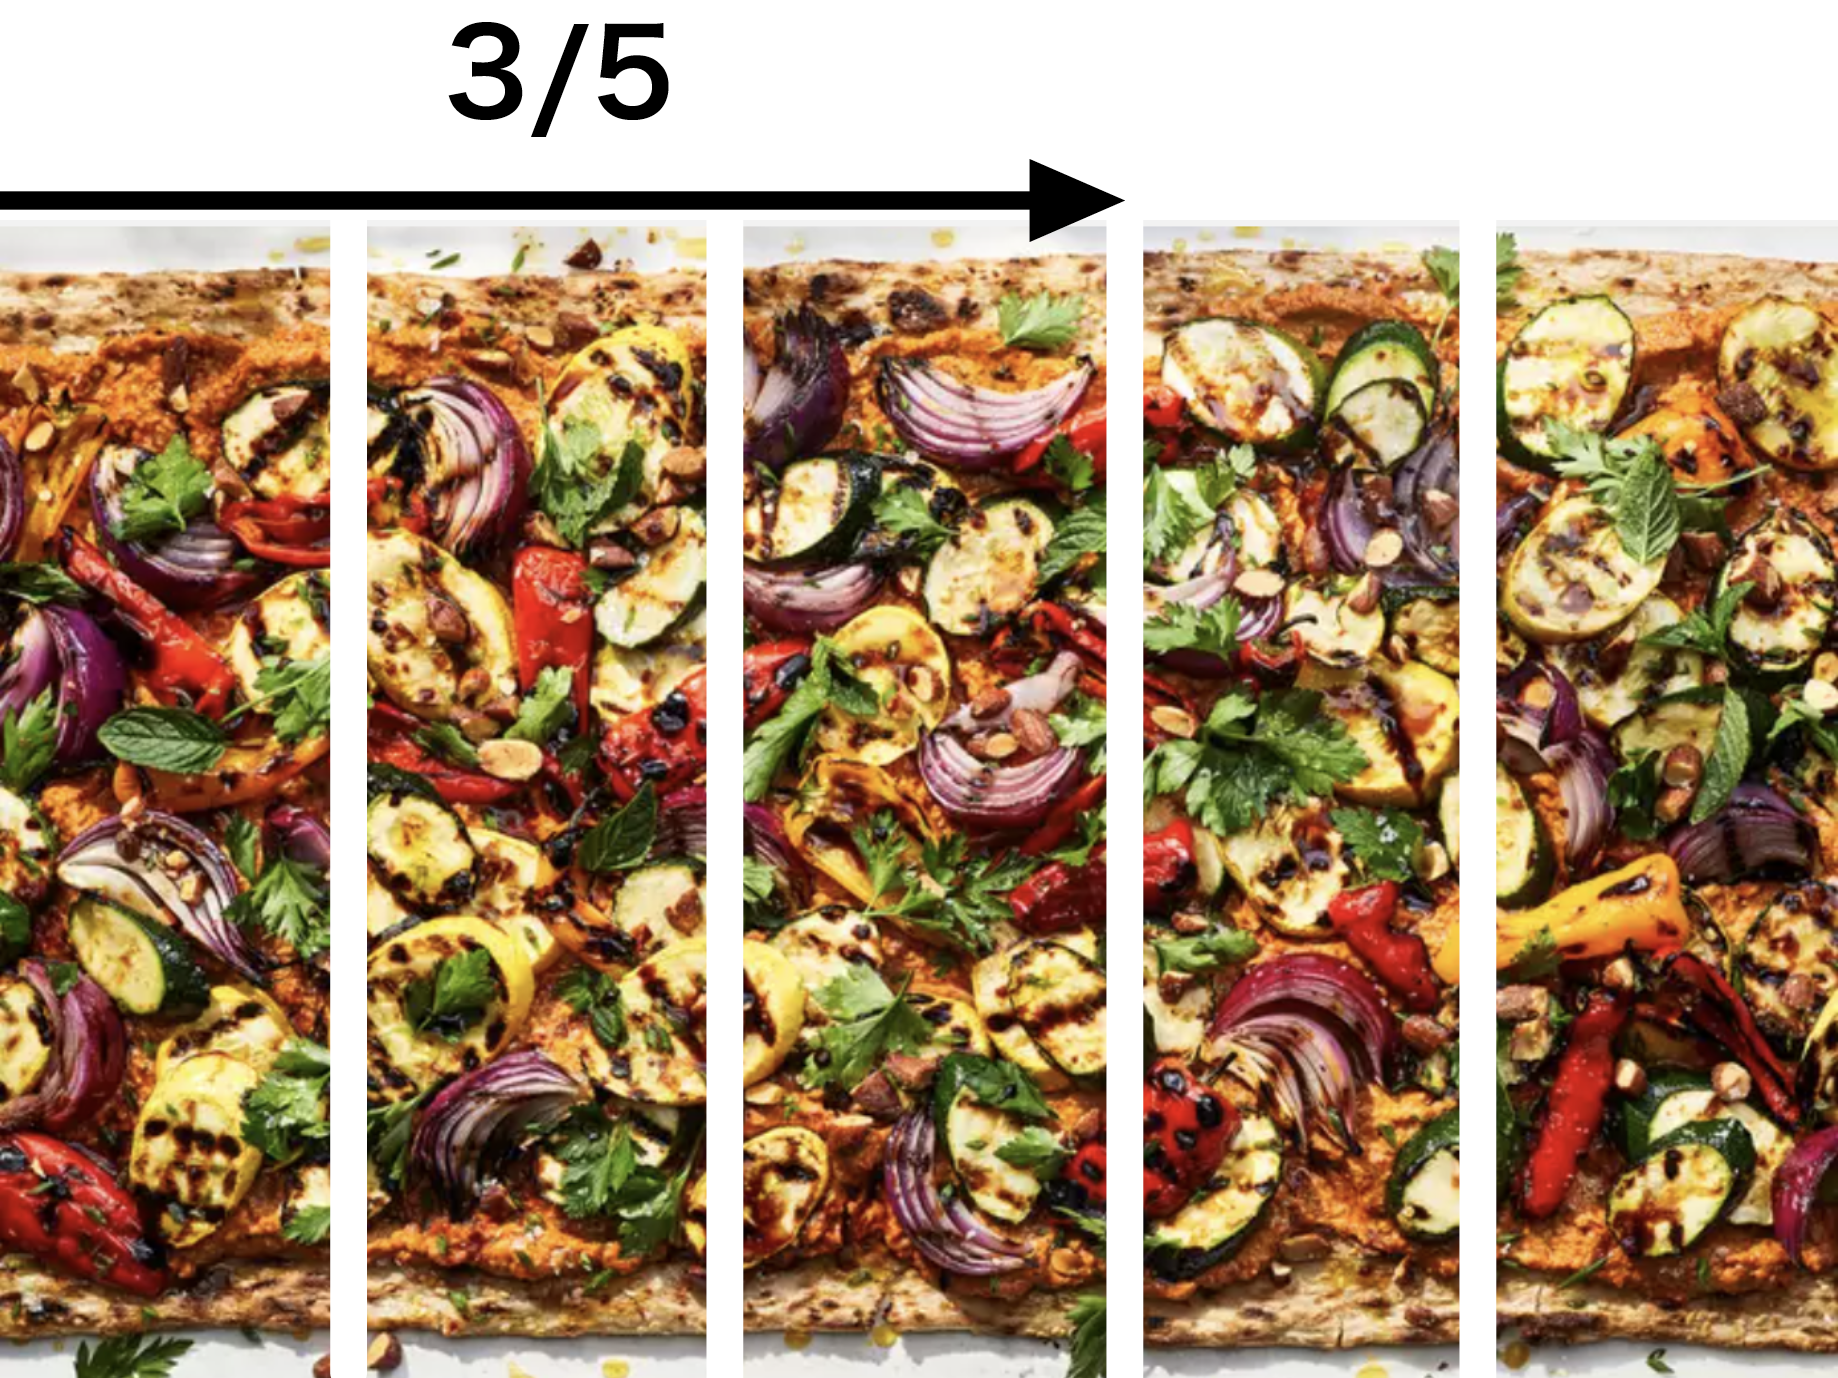
\includegraphics [width = 5in] {Flatbread slices.png}}
\vspace{.25in}
\end{minipage}

Turns out the salad was pretty big and so I only ate 3 slides of flatbread.  One way to describe how much of the flatbread I ate is using the fraction $\frac{3}{5}$. 

When I mentioned my dinner to my friend Hayfa she had a strange response:  ``Last time I ate a flatbread at Piadina's I only ate $\frac{2}{3}$ of what you ate.'' I quickly figured it out that since I ate 3 slices and she ate $\frac{2}{3}$ of that, she must have eaten 2 slices, which we can calculate as
$$\frac{2}{3} \times 3 = 2 \div 3 \times 3 = 2$$

I started to obsesses over these fractions. Remember that I ate $\frac{3}{5}$ of the flatbread and Hayfa ate $\frac{2}{3}$ of what I ate.  So she must have eaten $\frac{2}{3}$ of $\frac{3}{5}$, right?  That means
$$ \frac{2}{3} \times \frac{3}{5} = \frac{2}{5}$$
Ah yes!  She ate 2 out of 5 slices, or $\frac{2}{5}$ of the flatbread. That's correct. 

You might remember that we multiply fractions by multiplying the numerator (top) and the denominator (bottom). Let's do that
$$ \frac{2}{3} \times \frac{3}{5} = \frac{2 \times 3}{3 \times 5} = \frac{6}{15}$$
Uh oh.  We got a different answer.

Wait a minute.  Check it out:  
$$ \frac{2}{5} = 2 \div 5 = .4 \text{ \quad and \quad}  \frac{6}{15} = 6 \div 15 = .4$$
Whew!  The fractions $\frac{2}{5} $ and $\frac{6}{15}$ are equal. 

\newpage %%%%%

\noindent
\begin{minipage}{.55 \textwidth}
To see why, consider what happens when I cut the flatbread the other direction twice.  Now the entire flatbread has 15 squares.  Hayfa ate 2 slices out of the original 5 slices total.  Or, equivalently, she at 6 squares out of 15 original squares. You may have heard of reducing or cancelling fractions, which is a way to remember what's happening here:
\end{minipage}
\hfill
\begin{minipage}{.4 \textwidth}
\hfill
\scalebox {.45} {\includegraphics [width = 5in] {Flatbread squares.png}}
\vspace{.25in}
\end{minipage}
\vspace{-.3in}

$$\frac{2 \times 3}{3 \times 5} = \frac{2 \times \cancel{~3~}}{ \cancel{~3~} \times 5} = \frac{2}{5}$$

In practice when we have to evaluate a product of fractions we can do it a couple of ways.  One way is to deal with each fraction separately:

$$\frac{2}{3} \times \frac{3}{5} = 2 \div 3 \times 3 \div 5 = .4$$

Another way is to calculate the top and bottom of the fraction and divide.  Notice how we need to use parentheses around the top and bottom of the fraction.

$$ \frac{2}{3} \times \frac{3}{5} = \frac{2 \times 3}{3 \times 5} = (2 \times 3)\div (3 \times 5) = .4$$

By the way, flatbreads at Piadina's are pricey:  \$17.49 each.  At that rate, what does each slice cost?  We can use a fraction
$$\frac{\$17.49}{5 \text{ slices}} = \$17.49 \div 5 = 3.498 \approx \$3.50 \text{ per slice}$$
Notice that the units on my answer are dollars per slice:  the units of the numerator (top) per the units of the denominator (bottom).  We sometimes even write the units themselves as a fraction: $\frac{\$}{\text{slice}}$

There will be a few times during this course where you encounter fractions.  Mostly we'll switch to decimal approximations right away.  

 \begin{center}
\line(1,0){300} %\line(1,0){250}
\end{center}

\section*{Homework}

\noindent \textbf{Start by doing Practice exercises \#1-4 in the workbook.}

\bigskip

\noindent \textbf{Do you know \ldots}

\begin{itemize} 
\item How we represent a part of a whole as a fraction? %\vfill
\item How to multiply fractions?  %\vfill
\item What``canceling'' a factor means? %\vfill
\item How fractions are related to division? %\vfill
\item How to calculate the decimal approximation of a fraction? %\vfill
\item How to compare two fractions using their decimal approximations? %\vfill
\item How the units of a fraction are determined?  %\vfill
\item When we need to use parentheses around the top (numerator) and bottom (denominator) to evaluate a fraction? %\vfill
 \item[~] \textbf{If you're not sure, work the rest of exercises and then return to these questions.  Or, ask your instructor or a classmate for help.} 
\end{itemize}

\subsection*{Exercises}

On each problem, write down what you enter into your calculator and don't forget to write the units on your final answer.  Challenge yourself to use one-line calculations. You are welcome to calculate the answer step-by-step to check.

\begin{enumerate} 
\setcounter{enumi}{4}

\item In our flatbread example, the flatbread was served cut into 5 slices and we cut it lengthwise into 15 squares. 
\begin{enumerate}
\item Use our flatbread example to explain why $\frac{12}{15} = \frac{4}{5}$ and confirm by calculating the decimals. 
\item Use our flatbread example to explain why $\frac{10}{15} = \frac{2}{3}$ (hint:  think of very long strips!) and confirm by calculating the decimals.
\end{enumerate}

\item Auriel is making porridge but doesn't want too much.  Last time she cut the recipe in half, but that was too little. Auriel has decided that making $\frac{3}{4}$ of the recipe will be just right.  Figure out how much of each ingredient Auriel needs.  Report each answer as both a fraction and a decimal.

\begin{enumerate}
\item The original recipe calls for 5 ounces of skim milk.
\item The original recipe calls for $\frac{1}{2}$ cup oats.
\item The original recipe calls for $\frac{2}{3}$ cup of water.
\item The original recipe calls for $\frac{1}{3}$ cup of raisins.  
\end{enumerate}

\item A diver bounces on a 3-meter springboard.  Up she goes.  A somersault, a twist, and then whoosh, into the water.  \hfill \emph{Story also appears in 1.3.}
\begin{enumerate}
\item At .2 seconds after take-off she was 3.88 meters above the water.  Her initial speed can be calculated as 
$$\frac{3.88-3}{.2}$$
Find the diver's speed and don't forget the units.
\item At .4 seconds after take-off she was 4.38 meters above the water.  Her speed then can be calculated as 
$$\frac{4.38-3.88}{.4-.2 }$$
Find the diver's speed and don't forget the units.
\item Which speed is larger? Explain why that might make sense in the story.
\end{enumerate}

\item The football coach wants everyone to sprint three-quarters of a mile, up and back on the field which is labeled in years.  \hfill \emph{Story appears in 1.4 \#7.}
\begin{enumerate}
\item Find the number of yards by calculating
$$\frac{3}{4} \text{ miles}
\star
  \frac{5,280 \text{ feet}}{1 \text{ mile}}
\star
  \frac{1 \text{ yard}}{3 \text{ feet}} = \frac{3 \times 5280}{4 \times 3}$$
  \item Approximately how many times will the players need to run up and back on the field.  The field is 100 yards long so ``up and back'' is 200 yards.  
  \end{enumerate}



  


\end{enumerate}

\bigskip

\noindent \textbf{When you're done \ldots}

\begin{itemize}
\item Don't forget to check your answers with those in the back of the textbook. 
\item Not sure if your answers are close enough? Compare with a classmate or ask the instructor.  
\item Getting the wrong answers or stuck on a problem?  Re-read the section and try the problem again.   If you're still stuck, work with a classmate or go to your instructor's office hours.
\item It's normal to find some parts of some problems difficult, but if all the problems are giving you grief, be sure to talk with your instructor or advisor about it.  They might be able to suggest strategies or support services that can help you succeed.
\item Make a list of key ideas or processes to remember from the section.  The ``Do you know?'' questions can be a good starting point.
\end{itemize}

 
\section{Prelude: Powers and Roots}

Noah is very proud of his sobriety.  He credits some of his success to handicrafts, like beading.  He finds the steady, repetitive work of stringing beads one by one (or, actually, Noah prefers two by two) to be a calming practice and he enjoys flexing his artistic creativity.  

Noah's mom also enjoys handicrafts and would like to build a small glass box to hold some of Noah's beads. To keep things simple she has decided that the box will be a cube, meaning it will have the same length, width, and height.  Plus, the cube has long been the symbol of regeneration and stability but also of limitations and boundaries -- a fitting recovery gift.

She could make a small box that's $2 \times 2 \times 2$.  That's pronounced ``2 by 2 by 2'' and means 2 inches long, 2 inches wide, and 2 inches tall.  Such a small box would hold $2 \times 2 \times 2 =  8$ cubic inches of beads, which is around 2/3rd of a cup (not much).

What if Noah's mom made a box that was $5 \times 5 \times 5$ instead?  That box would hold $5 \times 5 \times 5 = 125$ cubic inches of beads, which is just over 2 liters of beads. Similarly a $10 \times 10 \times 10$ box would hold $10 \times 10 \times 10 = 1000$ cubic inches of beads, or about 4 gallons of beads. In case you're curious about the units here, there's about 14.4 cubic inches per cup,  61 cubic inches per liter, and 231 cubic inches per gallon.  

When we multiply a number by itself, like $$\underbrace{2 \times 2 \times 2}_{3 \text{ times}}$$ we say that we are raising 2 \textbf{to the power of} 3.  The number 3, which counts how many times we multiply 2 by itself, is called the \textbf{power} or \textbf{exponent}. 

On a calculator we can use the $\land$ key.  Try for yourself:
$$2 \land 3 = \underbrace{2 \times 2 \times 2}_{3 \text{ times}} = 8$$
$$5 \land 3 = \underbrace{5 \times 5 \times 5}_{3 \text{ times}} = 125$$
$$10 \land 3 = \underbrace{10 \times 10 \times 10}_{3 \text{ times}} = 1000$$
No key marked $\land$? Look for a key marked $x^y$ or $y^x$ instead. Can't find that either?  Ask a classmate or your instructor for help.

We can even do higher powers for practice:

$$3 \land 4 = \underbrace{3 \times 3 \times 3 \times 3}_{4 \text{ times}} = 81$$
$$2 \land 10 = \underbrace{2 \times 2 \times 2 \times 2 \times 2 \times 2 \times 2 \times 2 \times 2 \times 2}_{10 \text{ times}}= 1024$$
Speaking of which,  Noah thought it was fitting it is that his mom was using mathematical higher powers to build the glass box since learning to trust in a spiritual higher power was so important to his recovery.

Noah would like the box to hold 1 gallon of beads which is about 231 cubic inches.  What size cube box should his mom make?  She wants a number, let's call it $n$, so that an $n \times n \times n$ box will hold 231 cubic inches.  That means she needs $$n \times n \times n = 231$$ or, equivalently, $$n \land 3 = 231$$

Noah's mom can try to guess what number $n$ should be.  She wants a box that's bigger than $5  \times 5 \times 5$ but smaller than $10 \times 10 \times 10$.  Her first guess is $n=7$ inches, meaning the box will be $7 \times 7 \times 7$.  That box would hold $$7 \times 7 \times 7 = 7 \land 3 = 343 \text{ cubic inches}$$ which is too big.  How about $n = 6.5$ inches so the box would hold $$6.5 \times 6.5 \times 6.5 = 6.5 \land 3  \approx 274 \text{ cubic inches}$$ which is still too big. After a few more guesses she tries $n = 6.2$ so the box would hold $$6.2 \times 6.2 \times 6.2 = 6.2 \land 3 \approx 238 \text{ cubic inches}$$ Aha!  She will make a box that's approximately $6.2 \times 6.2 \times 6.2$.

That was a lot of guessing.  Turns out there's a name for the answer.  We write $$n = \sqrt[3]231$$ and say that the dimension we are looking for is the 3rd \textbf{root} of 231.  

We can use our calculator to find roots.  For example, if you have a key that says $\sqrt[x]{y}$ then you can enter
$$3 \sqrt[x]{y} ~231 =  6.1357...$$
Different calculators label the roots key differently.  For example, you may have to use one of the 2nd, Shift, or Inv key with the $\land$, $y^x$, or $x^y$ key.  On a graphing calculator, you may have to enter MATH mode.  

For practice, try evaluating the following roots on your calculator. Feel free to ask a classmate or your instructor for help if you can't figure it out.

$$\sqrt[3]{125} = 3 \sqrt[x]{y}~ 125= 5$$
$$\sqrt[3]{1000} = 3 \sqrt[x]{y}~ 1000 = 10$$
$$\sqrt[4]{81} = 4 \sqrt[x]{y}~ 81 = 3$$
$$\sqrt[10]{1024} = 10 \sqrt[x]{y}~ {1024} = 2$$

By the way, $n \land 3$ is sometimes called $n$ \textbf{cubed} and $\sqrt[3]{~}$ is referred to as the \textbf{cube root}.  That terminology comes from the fact that the $n \times n \times n$ cube has volume $n \times n \times n = n \land 3$, as in our example.  Also note that the units on volume which are inches $\times$ inches $\times$ inches are called \textbf{cubic inches}.

Similarly, $n \land 2$ is called $n$ \textbf{squared} and $\sqrt{~}$ (which is shorthand for $\sqrt[2]{~}$) is referred to as the \textbf{square root}.  Some calculators have a separate key for the square root.  That terminology comes from the fact that an $n \times n$ square has area $n \times n = n \land 2$.  And a square that was $n \times n$ in inches would have area measured in inches $\times$ inches, which are called \textbf{square inches}.
%See Sections 2.3, 2.4, and 3.3
%
%For problem 4 in workbook (and one in homework), perhaps use a growth factor formula example???

 \begin{center}
\line(1,0){300} %\line(1,0){250}
\end{center}

\section*{Homework}

\noindent \textbf{Start by doing Practice exercises \#1-4 in the workbook.}

\bigskip

\noindent \textbf{Do you know \ldots}

\begin{itemize}
\item What the square, cube, or higher power of a number means? %\vfill
\item How to calculate powers of a number using a calculator? %\vfill
\item What the square root, cube roots, or higher root of a number means? %\vfill
\item How to calculate roots of a number using a calculator? %\vfill
 \item[~] \textbf{If you're not sure, work the rest of exercises and then return to these questions.  Or, ask your instructor or a classmate for help.} 
\end{itemize}

\subsection*{Exercises}

\begin{enumerate} 
\setcounter{enumi}{4}

\item Remember Noah's mom from our story?  She was making a glass box that is $n \times n \times n$ where the length $n$ is measured in inches.
\begin{enumerate}
\item How many cubic inches of beads would the box hold if it's $8 \times 8 \times 8$? What if the box were $7.5 \times 7.5 \times 7.5$ instead?  You can first find the answers by multiplying on your calculator, but then challenge yourself to use the power key.
\item Use guessing to approximate the dimension of a box that would hold 400 cubic inches of beads. Just guess to the nearest one decimal place. Again, practice using the power key.
\item Use cube roots and your calculator to figure out the dimension of a box that would hold 400 cubic inches of beads, to the nearest one decimal place.  Does your answer agree with part (b)?  (It should.)
\end{enumerate}

\item Creeping Charlie is a low-growing weed that spreads quickly, doubling the area it covers each year.  If there are 7 square feet of Creeping Charlie in my lawn now, how much of my lawn will be covered by Creeping Charlie in 1 year? In 2 years? In 10 years?  (Try to answer that last one using powers)

\item Saboor is working on a needlepoint that will be a 1 foot by 1 foot square.  The mesh grid comes in different sizes.   For example, a 13-count mesh has 13 holes per inch which is $13 \times 12 =  156$ holes per foot. If she uses a 13-count mesh, then the piece will have $156 \times 156 = 156 \land 2 = 24,336$ holes.
\begin{enumerate}
\item How many holes does a 1 foot by 1 foot square mesh grid have if she uses a 10-count mesh instead which has 10 holes per inch? \vfill
\item What count mesh will have 10,000 holes?  First find the holes per foot by calculating $\sqrt{10000}$.  Then divide by 12 to find the holes per inch. \vfill
\end{enumerate}

\item A set of sterling silverware was valued at \$800 in 1920, and the value increased by around 3\% per year thereafter. \emph{Story appears in Section 5.1}
\begin{enumerate}
\item What was the value in 1921?  Remember, to find 3\% of a number we multiply by $3 \div 100 = .03$. %\vfill
\item What was the value in 1922?  Don't forget to use your answer to part (a) to calculate the new increase in value. %\vfill
\item It turns out there's a quicker way to find the answers to parts (a) and (b).  Calculate $800 \times 1.03=$ and $800 \times 1.03 \times 1.03 =$.   Note:  we will discuss this shortcut in greater detail in Section 2.2  %% Section on First look at exponentials
%\vfill
\item In general, we can find the value of the silverware after $Y$ years by calculating $$800 \times \underbrace{1.03 \times 1.03 \times \cdots \times 1.03}_{Y \text{ times}} = 800 \times 1.03 \land Y =$$ 
Use this powers method to find the value of the sterling in 1957.  Hint: $Y = 1957-1920 = 37$ years. %\vfill
\item Use this powers method to find the value of the sterling in 1990. %\vfill
\item Use this powers method to find the value of the sterling in 2023. %\vfill
\end{enumerate}

\end{enumerate}

\bigskip

\noindent \textbf{When you're done \ldots}

\begin{itemize}
\item Don't forget to check your answers with those in the back of the textbook. 
\item Not sure if your answers are close enough? Compare with a classmate or ask the instructor.  
\item Getting the wrong answers or stuck on a problem?  Re-read the section and try the problem again.   If you're still stuck, work with a classmate or go to your instructor's office hours.
\item It's normal to find some parts of some problems difficult, but if all the problems are giving you grief, be sure to talk with your instructor or advisor about it.  They might be able to suggest strategies or support services that can help you succeed.
\item Make a list of key ideas or processes to remember from the section.  The ``Do you know?'' questions can be a good starting point.
\end{itemize}


\section{Prelude: Algebraic Notation}

Minnesota had 35.5 inches of precipitation (rain and snow) in 2022, setting a new record.  It is difficult to predict the weather.  

One report estimated that precipitation would increase an average of .2 inches per year.  If that report is accurate then in 2032 (after 10 years) we would expect total precipitation to be around $$35.5 + 10 \times .2 = 37.5 \text{ inches}$$
We can use the letter $Y$ to represent the number of years in the future (since 2022).  

After $Y$ years, we would expect total precipitation (in inches) to be around $$35.5 + Y \times .2$$
This expression generalizes our earlier calculation, replacing the 10 years by the $Y$ years. This expression is often written as $$35.5 + .2Y$$
Notice that we are writing the number (.2) before the letter ($Y$).  Also, we are not writing the multiplication symbol ($\times$) at all!  It is something you just need to know:  that $.2Y$ really means $.2 \times Y$.  That shorthand is an example of algebraic notation.

Another report estimated that precipitation would increase about 0.5\% per year.  Notice that percentage is less than 1\%.  It is much more complicated to figure out what to expect in 2032 (after 10 years), but following some examples we saw in the last section, it turns out that we can calculate the predicted precipitation to be $$35.5 \times 1.005 \land 10 = 37.3154... \approx 37.3 \text{ inches}$$

After $Y$ years, we would expect total precipitation (in inches) to be around $$35.5 \times 1.005 \land Y$$
This expression generalizes our earlier calculation, replacing the 10 years by the $Y$ years.  This expression is often written as $$35.5*1.005^Y$$
Notice that we are writing the exponent as a superscript (meaning raised up and a little smaller).  Also notice that we have replaced the usual multiplication symbol $\times$ with an alternative symbol $*$.  That's because $\times$ looks like the letter $X$ which is sometimes used in algebra.  This shorthand is another example of algebraic notation.  The expression can also be written without the $*$ symbol as  $$35.5(1.005^Y)$$
where now we need to know that the number before the parentheses is multiplied.

For a little more practice with algebraic notation, recall that Piadina's flatbread cost \$17.49 and is usually cut into 5 slides.  At that rate it cost $$17.49 \div 5 = \$3.50$$ per slice.  If there were $S$ slices, then we can replace the 5 slices by $S$ slices and calculate that the flatbread cost $$17.49 \div S$$ in dollars per slice.  In algebraic notation, we write the division as a fraction instead 
$$ \frac{17.49}{S}$$

One more piece of terminology.  When we have an expression, like $ \frac{17.49}{S}$ and we want to know the value when $S$ is a particular value, we say that we are \textbf{evaluating} the expression.  Suppose we want to know the price per slice if Piadina's cut their flatbread into 4 slices instead.  That means we want to evaluate the expression $ \frac{17.49}{S}$ when $S = 4$ slices.  

The first step in the evaluation process is to replace the letter by its value and we write that value in parentheses.  Thus we would have $$\frac{17.49}{(4)}$$ The second step is to replace the algebraic notation with the arithmetic notation, which is usually what we enter into the calculator:
$$17.49 \div (4)$$
It turns out that we do not need the parentheses around the 4 so we can simply calculate $$ 17.49 \div 4 = 4.3725 \approx \$4.37 \text{ per slice}$$

 \begin{center}
\line(1,0){300} %\line(1,0){250}
\end{center}

\section*{Homework}

\noindent \textbf{Start by doing Practice exercises \#1-4 in the workbook.}

\bigskip

\noindent \textbf{Do you know \ldots}

\begin{itemize}
\item Where multiplication can be hidden in algebraic notation? %\vfill
\item How powers are written in algebraic notation?% \vfill
\item How division is written in algebraic notation? %\vfill
\item What the word evaluate means? %\vfill
\item How to evaluate an algebraic expression on your calculator? %\vfill
 \item[~] \textbf{If you're not sure, work the rest of exercises and then return to these questions.  Or, ask your instructor or a classmate for help.} 
\end{itemize}

\subsection*{Exercises}

\begin{enumerate} 
\setcounter{enumi}{4}

\item There were two different predictions of total precipitation.
\begin{enumerate}
\item What does the first report predict for total precipitation in 2042 (when $Y=20$) using the expression $35.5 + .2Y$?
\item What does the second report predict for total precipitation in 2042 (when $Y=20$) using the expression $35.5(1.005^Y)$?
\end{enumerate}


\item When the Nussbaums planted a walnut tree it was 5 feel tall. It has grown around 2 feet a year. If we know that it's been $Y$ years since they planted the tree, we can figure out that the height of the tree is $5+2Y$ feet.
 
 \hfill \emph{Story also appears in 0.2 \#7, 0.4 textbook, and 1.1 \#5(a)}  
\begin{enumerate}
\item Use this expression to figure out the height of the tree after 18 years.
\item What does $2Y$ mean in the expression $5+2Y$?
\end{enumerate}

\item A set of sterling silverware was valued at \$800 in 1920, and the value increased around 3\% per year thereafter.  We can calculate the value of the silverware after $Y$ years as $800 *1.03 ^ Y$. \hfill \emph{Story also appears in 0.6 \#8 and 5.1 textbook}
\begin{enumerate}
\item Use this expression to calculate the value of the silverware in 1990.  (Use $Y = 1990-1920 = 70$)
\item What does the $1.03^Y$ mean in the expression $800 *1.03 ^ Y$?
\item What does the symbol $*$ mean in the expression $800 *1.03 ^ Y$?
\item There are other ways to write this expression including $800 (1.03 ^ Y)$ and $800 (1.03) ^ Y$.  Evaluate each of these expressions at $Y=70$. You might not need to type in the multiplication.  Experiment to see what your calculator needs.
\end{enumerate}

\item The lake by Rodney's condo was stocked with bass (fish) 10 years ago.  There were initially 400 bass introduced.   \hfill \emph{Story also appears in 3.3 Exercises and 5.5 \#9}

\begin{enumerate}
\item One potential expression for the number of bass after $Y$ years is $$4000 - 3600*.78^Y$$ What does this equation say the number of bass should be now? Hint: that means $Y = 10$ years.
\item Another potential expression for the number of bass after $Y$ years is
$$\frac{4000}{1 + 9*.78^Y}$$
What does this equation say the number of bass should be now?  Since we're using a very different equation, we will get a very different answer.  Don't forget to put parentheses around the bottom of the fraction.
\item If there are actually 2500 fish in the lake now, which expression is closer to correct?
\end{enumerate}

\item Zahra needs to complete 62 more hours of classroom observation before she is eligible to student teach.  She plans to observe at a local school on Thursdays from 8:00 AM-1:30 PM, which is 5.5 hours/week. After $W$ weeks, Zahra will have $62-5.5W$ hours left.  \hfill \emph{Story appears in 0.2 textbook}
\begin{enumerate}
\item How many hours will Zahra have left after 4 weeks? Evaluate this expression to find the answer.
\item What does the $5.5W$ mean in the expression $62-5.5W$?
\item What does the $-$ mean in the expression $62-5.5W$?  Remember there are two similar looking operations: subtraction and negation.
\end{enumerate}

\item Saboor is working on a needlepoint that will be 1 foot by 1 foot square. The mesh grid comes in different sizes.  For example, a 13-count mesh has 13 holes per inch which is $13 \times 12=156$ holes per foot.  If she uses a 13-count mesh, then the piece will have $156 \times 156 = 156 \land 2 = 24,336$ holes. There are other sizes mesh to choose from.  A $C$-count mesh has $12C$ holes per foot and $(12C)^2$ holes total. 

\hfill \emph{Story also appears in 0.6 \#7}
\begin{enumerate}
\item Evaluate the expression $(12C)^2$ when $C=13$. Don't forget the units.
\item Evaluate the expression $(12C)^2$ when $C=10$ to count the total number of holes in a 10-count mesh.
\item What does the $12C$ mean in the expression $(12C)^2$?  
\item If we forgot the parentheses and typed in $12 \times 10 \land 2$, what answer would we get and what is the calculator doing differently?
\end{enumerate}

\end{enumerate}

\bigskip

\noindent \textbf{When you're done \ldots}

\begin{itemize}
\item Don't forget to check your answers with those in the back of the textbook. 
\item Not sure if your answers are close enough? Compare with a classmate or ask the instructor.  
\item Getting the wrong answers or stuck on a problem?  Re-read the section and try the problem again.   If you're still stuck, work with a classmate or go to your instructor's office hours.
\item It's normal to find some parts of some problems difficult, but if all the problems are giving you grief, be sure to talk with your instructor or advisor about it.  They might be able to suggest strategies or support services that can help you succeed.
\item Make a list of key ideas or processes to remember from the section.  The ``Do you know?'' questions can be a good starting point.
\end{itemize}



 \section{Prelude: Scientific Notation}

Tara is working on a big project at work.  She wants to back up her files to her online drop box. The site says she has 72 GB of memory remaining.  Tara has about 200 files at an average of 42.3 MB each that she would like to upload.  Will she have room?

To answer Tara's question we need to know that GB is short for ``gigabyte'' and MB is short for ``megabyte.''  A \textbf{byte} is a very small unit of computer memory storage space just enough for about one letter.  You may have heard the word ``mega'' used to mean ``really big.''  There's a reason for that.  \textbf{Mega} is short for 1 million.  That's pretty big.  But \textbf{giga} stands for 1 billion, so that's even bigger. So, really
\begin{center}
\begin{tabular} {lclcr} 
\textbf{megabyte} &$=$&1 \textbf{ million bytes} &$=$&$ \text{1,000,000 bytes}$\\
\textbf{gigabyte} &$=$& 1 \textbf{ billion bytes} &$=$& $\text{1,000,000,000 bytes}$\\ 
\end{tabular}
\end{center}

What all this means is Tara has
$$72\text{ GB} = 72 \text{ billion bytes} = \text{72,000,000,000 bytes}$$
of memory remaining.
She would like to save 200 files at 42.3 MB each which comes to
$$200 \times 42.3 = \text{8,460 MB}$$
which is really 
$$ \text{8,460 MB} = \text{8,460 million bytes} = \text{8,460,000,000} \text{ bytes}$$
$$= 8.46 \text{ billion bytes} = 8.46 \text{ GB }$$
So Tara wants to store less than 9 GB of information and she has 72 GB remaining.  She has plenty of room.  Save away!

Really large numbers, like \text{8,460,000,000}, are awkward to read and awkward to work with.  Words like million and billion or metric prefixes (words like mega and giga)  allow us to rewrite these large numbers in a way that's much easier both to read and to work with.  There's another option that's used often in the sciences (and by your calculator).  To explain it we need to understand powers of 10.

 Perhaps you know what happens when we multiply a number by 10, like
$ 5 \times 10 = 50$ or, more appropriate to our example, $$ 8.46 \times 10 = 84.6$$
The effect of multiplying by 10 is to move the decimal point one place to the right.
When we multiply by \text{1,000} we get
$ 5 \times \text{1,000} = \text{5,000} $ or, for our example, $$8.46 \times \text{1,000} = \text{8,460}$$
The effect of multiplying by \text{1,000} is to move the decimal point three places to the right.
The connection is that $$10^3=10 \times 10 \times 10  =\text{1,000}$$
Each $\times 10$ has the effect of moving the decimal point one place to the right so $\times \text{1,000}$ has the same effect as multiplying by 10 three times, so the decimal point moves three places to the right.
That means 
\begin{eqnarray*}
\text{8,460,000,000} & = & 8.46 \underbrace{\hbox{$\times 10 \times 10  \times 10  \times 10  \times 10  \times 10  \times 10  \times 10  \times 10 $}}_{\hbox{\begin{tiny} 9 times \end{tiny}}}  \\  %HSPACE
& = & 8.46 \ast 10^ 9 \\  
\end{eqnarray*} 
\vspace{-.5in} %VSPACE

This shorthand is called \textbf{scientific notation}.  The base is always 10.  The exponent is always a whole number.  The number out front, like 8.46 in our example, is always between 1 and 10, which means there's exactly one digit before the decimal point (and any others must come afterwards).  It is customary to use $\times$ instead of $\ast$ in scientific notation, so we should write
$$8.46\times10^9$$

As another example, we saw earlier that $$\text{5,000} = 5 \times \text{1,000} = 5 \times 10^3$$
You can check that  $$5 \times 10 \wedge 3 = 5000$$
 
Back to our large number.  Enter $$8.46 \times 10 \wedge 9=$$
What do you see?  Some calculators correctly show $\text{8,460,000,000}$ while other calculators report the number back in scientific notation, which is not particularly useful. (Sigh.)  

Let's try a number so big that (nearly) every calculator will switch to scientific notation.  Enter $$2.7\times 10 \wedge 30=$$
Look carefully at the screen.  Your calculator might display something like 
$$\boxed{~2.70000000 \quad \text{\begin{footnotesize}E \end{footnotesize}}~30~} \text{ \quad or \quad } \boxed{~2.70000000 \quad _{ \times \text{\begin{tiny}10 \end{tiny}}}~30~}$$ 
Whatever shorthand your calculator uses, you should write $$2.7 \times 10^{30}$$

Interested in what that number is in our usual decimal notation?  It's
$$2, \underbrace{ \hbox{$\text{700,000,000,000,000,000,000,000,000,000} $}}_{\hbox{\begin{tiny} decimal point moves 30 places \end{tiny}}}$$

Enough of that. Poor Tara is pulling her hair out over this project.  Well, not literally, but she is quite frustrated over how slowly the project is going.  She wonders: how thick is a human hair?  

Turns out that a typical human hair is about $.00012$ meters across.  Very small numbers are also awkward to read and awkward to work with.  In this section, we write  $.000~12$ where the strange-looking space is to help you read the number.  
 
We can also describe really small numbers using scientific notation.  Perhaps you know what happens when we divide a number by 10, like
$ 50 \div 10 = 5$ or, more appropriate to our example, $$ 1.2 \div 10 = .12$$
The effect of dividing by 10 is to move the decimal point one place to the left.
If we divide by \text{1,000,000} instead, we get
$$ 1.2 \div \text{1,000,000} = .000~001~2 $$ 
The connection is that $$ \text{1,000,000} = 10 \wedge 6  $$
and so dividing by \text{1,000,000} moves the decimal point six places to the left.  Notice that we have to introduce zeros as placeholders.

The width of a hair was .00012 meters.  To get that number from 1.2, we need to move the decimal point 4 places to the left.  $$1.2 \div 10^4 = 1.2 \div \text{10,000} = .000~12$$
The shorthand for dividing by a power is to use negative exponents.  For example
$$ \div 10^4 = \times 10^{-4}$$
It has nothing to do with negative numbers.  It's just a shorthand.
The point of this calculation was that $$.00012= 1.2 \ast10^{-4}$$
Use your calculator to check!

Once again we have scientific notation.  The base is still 10.  The exponent is still a whole number, although now it's negative.  The number out front, like 1.2 in our example, is still between 1 and 10, which means there's exactly one digit before the decimal point (and any others must come afterwards).  As before, we'll write $\times$ instead of $\ast$ to get: $$1.2 \times 10^{-4}$$


When you see a number written in scientific notation, the power of 10 tells you a lot.  For example, we saw that $8.46 \times 10^ 9 = \text{8,460,000,000}$ and $1.2 \times10^{-4} = .000~12 $.  A positive power of 10 says you have a big number, and a negative power of 10 says you're dealing with a very small number. 
\bigskip

\noindent \textbf{Do you know \ldots}

\begin{itemize}
\item What million, billion, and trillion mean?  
\item Why scientific notation is used?  
\item The standard format for scientific notation?  
\item That a positive exponent corresponds to a big number and a negative exponent corresponds to a tiny number?
\item How to convert from scientific notation to decimal?  
\item How your calculator reports numbers in scientific notation, and what (might be) different when you're reporting that number?  
 \item[~] \textbf{If you're not sure, work the rest of exercises and then return to these questions.  Or, ask your instructor or a classmate for help.} 
\end{itemize}

\subsection*{Exercises}

\begin{enumerate} 
\setcounter{enumi}{4}

\item \emph{Story also appears in 1.5 \#6}
\begin{enumerate}
\item Convert 1 million seconds into an understandable unit of time. 
\item Billy Bob wants to throw a party when he turns 1 billion seconds old. About how many years old will he be?
\item \emph{Bonus question:}  On what date were you or will you be 1 billion seconds old?  Don't forget leap years! \hfill \begin{footnotesize} Source:  Mathew Foss, North Hennepin Community College \end{footnotesize} % YES, only one t in Mathew.
\end{enumerate}  

\item \emph{Story also appears in 1.5 \#3} 
\begin{enumerate}
\item The planet Jupiter weighs approximately $\mathbf{1.9 \times 10^{27}}$ \textbf{kilograms}. Write out this number (with all the zeros).
\item The planet Mars weighs approximately $\mathbf{6.4 \times 10^{23}}$ \textbf{kilograms}. Write out this number (with all the zeros).
\item Which planet weighs more:  Jupiter or Mars?  Explain. 
\end{enumerate}

\item \begin{enumerate}
\item The SARS CoV-2 virus is approximately 125 nanometers wide which is 
$\mathbf{125 \times 10^{-9}}$ \textbf{meters} wide. Write out this number (with all the zeros).
\item The N95 mask prevents particles down to 0.3 microns which is 
$\mathbf{3 \times 10^{-6}}$ \textbf{meters} wide but not smaller. Write out this number (with all the zeros).
\item Can the N95 mask prevent the SARS CoV-2 virus?  Explain.
\end{enumerate}

\item  Rayka would like to approximate how many cells are in her body.  Use the following information: Rayka weighs 140 pounds, $1 \text{ gram} \approx 10^{15} \text{ cells}$ and $\text{1,000 grams} \approx \text{2.2 pounds}$.
\hfill \emph{Story also appears in 1.5 \#9}
\begin{enumerate}
\item How many cells are in Rayka's body?  Hint: this is a unit conversion question asking you to convert 140 pounds to cells.  Write your answer in scientific notation.
\item Rewrite your answer in the most appropriate unit:  millions ($10^6$), billions ($10^9$), trillions ($10^{12}$), quadrillions ($10^{15}$), or quintillions ($10^{18}$).
\end{enumerate}

\end{enumerate}

\bigskip

\noindent \textbf{When you're done \ldots}

\begin{itemize}
\item Don't forget to check your answers with those in the back of the textbook. 
\item Not sure if your answers are close enough? Compare with a classmate or ask the instructor.  
\item Getting the wrong answers or stuck on a problem?  Re-read the section and try the problem again.   If you're still stuck, work with a classmate or go to your instructor's office hours.
\item It's normal to find some parts of some problems difficult, but if all the problems are giving you grief, be sure to talk with your instructor or advisor about it.  They might be able to suggest strategies or support services that can help you succeed.
\item Make a list of key ideas or processes to remember from the section.  The ``Do you know?'' questions can be a good starting point.
\end{itemize}



 \section{Prelude: Logarithms}

Nearlywed, hellscape, bodycon, and woke.  Just a few new words added to dictionaries in 2023.  People love to create new words and phrases.  These new words spread through social media, music, and word of mouth.

I created a new word ``puzzlaxing'' meaning relaxing by doing puzzles. In one week, maybe 10 people will have heard of it.  After another week, perhaps 100 people.  Then 1,000 the next week, and so on.  How many weeks until 1 million people are have heard of my new word ``puzzlaxing"?

Notice that in 1 week is $10 = 10^1$ people, two weeks is $10^2 = 100$ people, three weeks is $10^3=1000$ people, and so on.  We are looking for a number $W$ where $10^W=1,000,000$ people.  Aha!  $10^6=1,000,000$ and so $W=6$ weeks from now.

Suppose we wanted to determine when 5,000 people had heard of ``puzzlaxing''.  That means we want a number $W$ where $10^W = 5,000$.  Now what?  The answer is somewhere between 3 and 4 weeks because $10^3=1,000$ and $10^4=10,000$.  That's probably a good enough answer -- between 3 and 4 weeks, but suppose we want the exact moment. 

Let's try guessing.  How about 3.5 weeks? 
$$10^{3.5} =10 \wedge 3.5 = 3,162.27... $$ 
which is much smaller than 5,000.  How about 3.7 weeks? 
$$10^{3.7} =10 \wedge 3.7 = 5,011.87.. $$ 
which is slightly bigger than 5,000.  I want to find the answer here so let's try 
$$10^{3.69}=10 \wedge 3.69= 4,897.78...$$ 
or finally 
$$10^{3.699}=10 \wedge 3.699= 5,000.34...$$ 
That's as close as I'm gonna guess. 

Okay, I'm curious. Is there an exact power of 10 that gives 5,000?  Your calculator should have a key that says ``log'' or maybe ``LOG''.  Try typing $$\log(5000)=  3.6989700043...$$
A small note here about parentheses.  Some calculators give the first parenthesis for free when you type log but you have to type the closing parenthesis in yourself.  

Check it out, that's the answer we were looking for 
$$10^{3.6989700043} =10 \wedge 3.6989700043 = \text{4,999.999~999~5853...} \approx 5,000$$
If we had kept more digits it would have been actually 5,000.

What is this log key doing?  First, log is short for logarithm base 10.  There are other bases, but 10 is what we'll focus on in this course.  Try these calculations:

\begin{eqnarray*}
\log (10) & = & 1 \\
\log (100) & = & 2 \\
\log (1,000) & = & 3 \\
\log (10,000) & = & 4 \\
\log (100,000) & = & 5 \\
\log (1,000,000) & = & 6 \\
\end{eqnarray*}
\vspace{-.5in} %VSPACE

What do you see?  In each case the logarithm is the number of zeros or, equivalently, it's the power of 10.  For example, 10,000 has 4 zeros and $10^4= 10,000$ and $\log(10,000) = \log(10^4)=4$. In other words, a logarithm is just an exponent. And logarithms help us find the exponent.  Makes sense.

What logs of numbers that aren't just powers of 10? Here are some examples.
\begin{eqnarray*}
\log (25) & = & 1.3979\ldots \\
\log (250) & = & 2.3979\ldots \\
\log (2,500) & = & 3.3979\ldots \\
\log (25,000) & = & 4.3979\ldots \\
\end{eqnarray*}
\vspace{-.5in} %VSPACE

To see what's happening we want to involve powers of 10.  Scientific notation will do that for us.  Let's write these numbers in scientific notation and see what we learn.  For example $ 25,000 = 2.5 \times 10^4$ and 
$$ \log( 25,000)=\log(2.5 \times 10 ^4)=4.3979\ldots \approx 4$$
Before we write down a general rule, let's check more numbers.

$$\log(7,420,000) = \log(7.42 \times 10^6)=6.870403905\ldots \approx 6$$ 
$$\log (4)=\log(4 \times 10^0)=0.602059991\ldots \approx 0$$ 
$$\log (.00917)= \log(9.17 \times 10^{-3}) = -2.037630664\ldots \approx -3$$
In every case we are rounding down, but it's always the same:

\begin{center}
log(number) $\approx$ power of 10 in the scientific notation for that number.
\end{center}

\noindent \textbf{Do you know \ldots}

\begin{itemize}
\item What a logarithm (base 10) means? 
\item How to evaluate logarithms (base 10) on a calculator? 
\item Which size numbers have a positive log and which have a negative log (base 10)?
\item The connection between logarithms (base 10) and scientific notation.
\item[~] \textbf{If you're not sure, work the rest of exercises and then return to these questions.  Or, ask your instructor or a classmate for help.}
\end{itemize}

\subsection*{Exercises}


%Find power of 10 that equals number when exact + and -
%Find power of 10 that equals number by successive approximations.
%Find power of 10 that equals number using logs
%Explain connection between logs and scientific notation

\begin{enumerate} 
\setcounter{enumi}{4}

\item According to our story, in approximately how many weeks will 30,000 people have heard of ``puzzlelaxing"?
\begin{enumerate}
\item Since 30,000 is between 10,000 and 100,000, what does that tell us about the answer?
\item Guess to try to find the answer, the number $W$ where $10^W = 30,000$.  It's okay to get the answer to one decimal place.
\item Use logs to find an exact answer.
\end{enumerate}

\item The intensity of a sound in decibels is calculated using a logarithm.  For example, a sound 100 times the level humans can hear has an intensity of 
$$10\log (100)= 10 \times \log(100)= 20\text{ decibels}$$
\begin{enumerate}
\item Calculate the intensity, in decibels, of a cat purring which averages about 300 times the level humans can hear using the formula $10\log(300)$.
\item Calculate the intensity, in decibels, of normal conversation which averages about 1 million times the level humans can hear using the formula $10\log(1,000,000)$.
\item Many young adults are at high risk of hearing loss because they crank the volume of music they're listening to, often to 2 trillion times the level humans can hear.  Calculate that intensity in decimals using the formula $10\log(2 \ast10^{12})$. Prolonged sound above 70 decibels may damage your hearing and any loud noise above 120 decibels can cause immediate harm to hearing.
\end{enumerate}

\item In 2021, Arrietty charged \$5,000 on her credit card to help pay tuition.  Her card charges interest at the rate of 20.7\% APR.   We are going to ignore any minimum payments or fees.
\begin{enumerate}
\item Arrietty was hoping to pay the debt back quickly, but in 2023 she had not paid any of the debt.  Calculate the amount due on that original charge using the formula $5000 \ast 1.207^2$.
\item If she continues to leave the debt unpaid, when will her debt pass \$10,000? As we'll see later, the answer is $\displaystyle \frac{\log(2)}{\log(1.207)}$ years after 2020.  Don't forget to the close the parentheses.  
\end{enumerate}

\item Darcy likes to use temporary hair color in wild colors.  Good thing it washes out.  Her best guess is that 8\% of the color washes out each time she shampoos her hair.   That means $100\% - 8\% = 92\%$ of the color remains after each shampoo.

\hfill \emph{Story also appears in 3.4 \#9}
\begin{enumerate}
\item What percentage of the color will be remain after Darcy washes her hair three times?  Calculate the percentage using the formula $100 \ast .92^3$.  
\item After how many shampoos will half of the color be gone?  As we'll see later, the answer is $\displaystyle \frac{\log(.5)}{\log(.92)}$.  Don't forget to the close the parentheses. 
\end{enumerate}
 

\end{enumerate}

\bigskip

\noindent \textbf{When you're done \ldots}

\begin{itemize}
\item Don't forget to check your answers with those in the back of the textbook. 
\item Not sure if your answers are close enough? Compare with a classmate or ask the instructor.  
\item Getting the wrong answers or stuck on a problem?  Re-read the section and try the problem again.   If you're still stuck, work with a classmate or go to your instructor's office hours.
\item It's normal to find some parts of some problems difficult, but if all the problems are giving you grief, be sure to talk with your instructor or advisor about it.  They might be able to suggest strategies or support services that can help you succeed.
\item Make a list of key ideas or processes to remember from the section.  The ``Do you know?'' questions can be a good starting point.
\end{itemize}




\chapter{Variables}

Believe it or not, algebra is useful.  Really useful. It's useful in later courses you might take in mathematics, statistics, science, social science, or business.  But it's also useful in real life.  A lot of what happens in the world around us is easier to understand using algebra.  That's what this course is all about:  using algebra to answer questions. 

In this first chapter, we will introduce the key concepts of variable and function that help us translate between problems stated in words and the mathematics explaining the situation.  We explain the important tools of units, tables, and graphs.  We also describe how functions change and use the rate of change to approximate answers to questions.  Throughout this chapter we keep a careful eye on evaluating the reasonableness of answers by connecting what we learn from algebra with our own life experience. After all, an answer to a real problem should make sense, right?

Some of our approach may feel very different to you.  It is possibly quite different from what you've seen in mathematics classes before.   It might take you a little time to get used to, but it will be worth it.

 
%\include{Approx_prelude}
      
\section{Variables and functions}

Things change, like the price of gasoline, and just about every day it seems.  What does it mean when the price of a gallon of gas drops from \$3.999/gal to \$3.299/gal?  The symbol / is short for ``per'' or ``for each,''  so that means each gallon costs
$$\$3.999-\$3.299=\$.70 = 70\text{\textcent}$$ less.  Does this 70\textcent \hspace{.05in}truly matter?

Before we answer that question, are you wondering why there's that extra 9 at the end of the price?  We might think a gallon costs \$3.99 but there's really a small 9 following it.  Sometimes that 9 is raised up slightly on the gas station sign.  You have to read the fine print.  What it means is an extra $ \frac{9}{10}$\textcent \hspace{.05in}for each gallon.  So the true price of a gallon gas would be \$3.999.  Gas costs a tiny bit more than you thought.  Good grief.

%For the record, the / symbol is short for ``per''.  So when we write \$3.999/gal we mean \$3.999 per gallon.  
%Sometimes we write this as a fraction instead:  $ \frac{\$3.999}{\text{gallon}}$.

Back to our question.  Does 70\textcent \hspace{.05in}truly matter to us?  Probably not.  Can't even buy a bag of potato chips for 70\textcent.  But, how often do you buy just one gallon of gas?  Typically you might put five, or ten, or even twenty gallons of gas into the tank.  We want to understand how the price of gasoline influences what it really costs us at the pump.  To do that let's compare our costs when we buy ten gallons of gas.  There's no good reason for picking ten; it's just a nice number to work with.

If gas costs \$3.999/gal and we buy 10 gallons, it costs 
$$10 \text{ gallons} \ast \frac{\$3.999}{\text{gallon}} = 10 \times 3.999  = \$39.99$$   
See how we described the computation twice?  First, with units, fractions, and $\ast$ for multiplication in what's sometimes called ``algebraic notation.''  Then, with just numbers and $\times$ for multiplication -- that's what you can type into a calculator.  % SU later, if have the appendices done, reference here.

 If gas drops to \$3.299/gal and we buy 10 gallons, it costs 
$$10 \text{ gallons} \ast \frac{\$3.299}{\text{gallon}} = 10 \times 3.299  = \$32.99$$
That's \$7 less.  For \$7 savings on gas you could buy that bag of potato chips, and an iced tea to go with it, and still have change. That amount matters.  I mean, especially since it's \$7 savings every time you put 10 gallons in the tank.

Gas prices have been changing wildly, and along with them, the price of 10 gallons of gas.  In mathematics, things that change are called \textbf{variables}.  The two variables we're focusing on in this story are
\begin{center}
\begin{tabular} {l} 
$P=$ price of gasoline (\$/gal) \\
$C= $ total cost (\$) \\ 
\end{tabular}
\end{center}
Notice that we gave each variable a letter name.  It is helpful to just use a single letter chosen from the word it stands for.  In our example, $P$ stands for ``price'' and $C$ stands for ``cost''.  In this course we rarely use the letter $X$ simply because so few words begin with $X$.  Whenever we name a variable ($P$) we also describe in words what it represents (the price of gasoline), and we state what units it's measured in (\$/gal).

In talking about the relationship between these variables we might say ``the cost depends on the price of gas,'' so $C$ depends on $P$.  That tells us that $C$ is the \textbf{dependent variable} and $P$ is the \textbf{independent variable}.  In general, the variable we really care about is the dependent variable, in this case $C$ the total amount of money it costs us.   The concept of dependence is so important that there's yet another word for it.  We say that $C$ is a \textbf{function} of $P$, as in  ``cost is a function of price.''  

Knowing which variable is independent or dependent is helpful to us.  To emphasize the dependence, we often make a notation next to the variable name.  
\begin{center}
\begin{tabular} {l} 
$P=$ price of gasoline (\$/gal) $\sim$ indep \\
$C= $ total cost (\$) $\sim$ dep \\ 
\end{tabular}
\end{center}
This labeling is rarely used outside this textbook, so add it in for yourself if you need it.  In some situations dependency can be viewed either way; there might not be one correct way to do it.  Labeling the dependence is extra important then, so anyone reading your work knows which way you are thinking of it.  

Given a choice, we usually assign dependence such that given a value of the independent variable, it is easy to calculate the corresponding value for the dependent variable.  In our example it's easy to use the price per gallon, $P$, to figure out the total cost, $C$.  We can work backwards -- from $C$ to $P$ -- but it's not as easy.  

For example, suppose we buy 10 gallons of gas and it costs \$28.99.  We can figure out that the price per gallon must be
$$P=\frac{\$28.99}{10 \text{ gallons}}= 28.99 \div 10 = \$2.899 \text{/gal}$$  Notice that we use the fraction as part of the algebraic notation, but we use $\div$ to indicate division on the calculator.  Your calculator key for division may be $/$ instead, which we reserve as a shorthand for ``per.''

From our experience we have a sense of what gas might cost.  In my lifetime, I've seen gas prices as low as 35.9\textcent \hspace{.05in}/gallon in the 1960s to a high of \$4.099/gallon recently.  This range of values sounds too specific, so it would sound better to say something general like \begin{center} ``Gas prices are (definitely) between \$0/gal and \$5/gal.'' \end{center} 

The mathematical shorthand for this sentence is $$0 \le P \le 5$$  The inequality symbol $\le$ is pronounced ``less than or equal to''.  Formally, the range of realistic values of the independent variable is called the \textbf{domain} of the function $C$.  In this text, we rarely write the domain because it's usually clear from the story what realistic values would be.  The exercises in this section ask you to do so for practice.

Be aware that there are often many different numbers in a story.  Some numbers are examples of values the variables take on, such as \$3.999/gal or \$39.99 in our example.  Other numbers are \textbf{constants}; they do not change (at least not during the story).  The one constant in our story is that we are always buying 10 gallons of gas.  Occasionally there are other numbers in a story that turn out not to be relevant at all, so be on the lookout.

Back to our story.  A report says that the average price of gasoline in Minnesota was  \$2.900/gal in 2010 and increased approximately 20\% per year for the next several years.  We would like to check what that says about the average price of gasoline in 2011 and 2012, say.  (It is unlikely that the price increase continued much longer at that rate.)

To understand what that report is saying, we need to remember how percents work.  Luckily, the word ``percent'' is very descriptive.  The ``cent'' part means ``hundred,'' like 100 cents in a dollar or 100 years in a century.  And, as usual, ``per'' means ``for each.''  Together, \textbf{percent} means ``per hundred.''  The number 20\% means 20 for each hundred.  Written as a fraction it is $\frac{20}{100}$.  Divide to get the decimal $20 \div 100 = 0.20.$   
$$\text{Think money:  }20\%\text{ is like }20\text{\textcent , and }0.20\text{ is like }\$0.20$$  
Bottom line:  20\%, $\frac{20}{100}$, and 0.20 mean exactly the same number.
$$20\% = \frac{20}{100} = 20 \div 100 = 0.20$$

To calculate the percent of a number we multiply by the decimal version.  For example,
$$20\% \text{ of } \$2.900 = 0.20 \times 2.900 = \$.58$$
The report says the price increased by 20\% each year, so by 2011 the price had increased an average of \$.58.  That's not what gas cost in 2011.  It's how much \emph{more} gas cost in 2011 compared to 2010.  To see what the report projected for the 2011 cost we need to add that increase on to the original 2010 price.
$$\$2.099 + \$0.58= \$3.48\text{ per gallon}$$
Sounds about right.  Expensive, to be sure, but fairly accurate.

For 2012, the price increased by 20\% again.  That means 20\% of what it was in 2011.  We can't just add \$.58 again.  That was 20\% of the 2010 value, and we want 20\% \emph{of the 2011 value}.  Going to have to calculate that.
$$20\% \text{ of } \$3.48 = 0.20 \times 3.48 = \$.696$$
so the projected 2012 value was $$\$3.48 + \$.696= \$4.176\text{ per gallon}$$
Yikes.

One last note.  The number 20\% in the report sounds like a rough approximation.  The report probably means the increase was around 20\%, maybe a little less, maybe a little more.  So our answers of \$3.48/gal and \$4.176/gal could be a little less or a little more too.  But they sound so perfectly correct.  To be safe, we really ought to round off these answers, to something more general like around \$3.50/gal in 2011 or approximately \$4.20/gal in 2012.  % Su cite appendix on rounding off/approx?

When we want someone reading our calculation to know that we mean approximately, not exactly, we use the \textbf{approximately equal to} symbol $\approx$.  We save the equal sign, =, for when we have not rounded off the number at all.  So, according to the report $P \approx \$3.50$/gal in 2011 and $P \approx \$4.20$/gal in 2012.  

A lot of realistic problems involve percentages and so we use them often in this text.

%\newpage

%%\section{Variables and functions}

\begin{center}
\line(1,0){300} %\line(1,0){250}
\end{center}

\section*{Homework}

\noindent \textbf{Start by doing Practice exercises \#1-4 in the workbook.}

\bigskip

\noindent \textbf{Do you know \ldots}

\begin{itemize}
\item The difference between a variable and a constant?
\item The information needed to ``name'' a variable?
\item Which variable is dependent and which variable is independent? 
\item What ``domain'' means?
\item How to calculate percent increase? 
\item[$\star$] The symbol for ``approximately equal to''? 
\item[$\star$] Why an approximate answer is often as good as we can get? 
\item[$\star$] When to round your answer up or down instead of off? 
\item[$\star$] What the term ``precisely'' refers to? 
\item[$\star$] How to decide how precisely to round your answer?

\hfill  $\star$ indicates question based on \emph{Prelude:  approximation}
\item[~] \textbf{If you're not sure, work the rest of exercises and then return to these questions.  Or, ask your instructor or a classmate for help.}
\end{itemize}

\subsection*{Exercises}

\begin{enumerate} 
\setcounter{enumi}{4}

\item  It's about time!  For each story, try to figure out the answer to the question(s).
\begin{enumerate}
\item The Nussbaums planted a walnut tree years ago when they first bought their house.  The tree was 5 feet tall then and has grown around 2 feet a year. The tree is now 40 feet tall.  How long ago did the Nussbaums plant their walnut tree?
\item After his first beer, Stephen's blood alcohol content (BAC) was already 0.04 and as he continued to drink, his BAC level rose 45\% per hour.  Note that $$45\% = \frac{45}{100} = 45 \div 100 = 0.45$$  What was Stephen's BAC after 1 hour?  After 2 hours?

\hfill \emph{Story also appears in 2.4 Exercises and 3.4 \#1}
\item When McKenna drives 60 mph (miles per hour) it takes her 20 minutes on the highway to get between exits, but when traffic is bad it can take her an hour.  How slow is McKenna driving when traffic is bad?  \emph{Hint:  can you figure out the distance between exits?}
\item The sun set at 6:00 p.m.\ today and I heard on the radio that it sets about 2 minutes earlier each day this time of year.  In how many days will the sun set at 4:30 p.m.?
\emph{Bonus question:  in what month is the story set?}

 \hfill \emph{Stories also appear in 1.1 \#4}
\end{enumerate}  

\item The temperature was 40$^\circ$F at noon yesterday downtown Minneapolis but it dropped 3$^\circ$F an hour in the afternoon.   \hfill \emph{Story also appears in 1.2 and 4.1 Exercises}
 \begin{enumerate}
 \item Which number is a constant in this story: the temperature (40) or the rate at which the temperature dropped (3)?
\item Name the variables, including units and dependence. 
\item When did the temperature drop below freezing (32$^\circ$F)?
\end{enumerate}  

\item Mrs.\ Nystrom's Social Security benefit was \$746.17/month when she retired from teaching in 2009. She had taught in elementary school since I was a girl.   Benefits have increased by 4\% per year.   \hfill \emph{Story also appears in 1.2 and 5.1 Exercises} 
\begin{enumerate}
\item Name the variables, including units and dependence. 
\item What was her benefit in 2012?
\item When will her benefit pass \$900/month?  A reasonable guess is fine.  
\end{enumerate}  

\item Between e-mail, automatic bill pay, and online banking, it seems like I hardly ever actually mail something.   But for those times, I need postage stamps. The corner store sells as many (or few) stamps as I want for 44\textcent~each but they charge a 75\textcent~convenience fee for the whole purchase.   \hfill \emph{Story also appears in 3.1 Exercises}
\begin{enumerate}
\item  Identify and name the variables, including the units.
\item Which variable is dependent and which is independent?
\item How many stamps could I buy for \$10?  Try to figure it out from the story.\end{enumerate} 

\item Sof\'ia bought her car new for \$22,500.  Now the car is fairly old and just passed 109,000 miles.  Sof\'ia looked online and estimates the car is still worth \$5,700.   

  \hfill \emph{Story also appears in Section 5.4} 
\begin{enumerate}
\item Identify and name the variables, including the units
\item Explain the dependence using a sentence of the form ``\underline{~\quad} is a function of \underline{~\quad}''
\item What is a realistic number of miles for a car to drive?  Express the domain as an inequality.
\item Sof\'ia  wonders when the car would be practically worthless, meaning under \$500.   Make a reasonable guess.
\end{enumerate} 

\item For each story, name the variables including units and dependence.
\begin{enumerate}
\item The closer you sit to a lamp, the brighter the light is. 

\hfill \emph{Story also appears in 2.3 and 3.3 Exercises.}
\item The thicker the piece of fish, the longer it takes to grill it.

\hfill \emph{Story also appears in 2.3 and 3.5 Exercises.}
\item Wind turbines are used to generate electricity.  The faster the wind, the more power they generate. \hfill \emph{Story also appears in 1.3, 2.4, and 3.3 Exercises.}

\end{enumerate}

\end{enumerate}



  %% ADD EXERCISES BACK IN LATER 
      
\section{Tables and graphs}

%Should any of the generic/abstract graph drawing should be here.  It can certainly move to an appendix instead, and then rewrite this section to cut quickly to the graph.

%% SU -- what should the standard number of boxes across and up be, for the purpose of this text.  Is there a standard graph paper template to use?
%GraphPaper.png is 24 across (same as this graph, by the way) and 16 up.

% In the DYK need a "ask your instructor" about what sorts of graphing technology are available.

Lung cancer, chronic bronchitis, bad breath, stains on your clothes, and the expense.  These are just a few of the consequences of smoking cigarettes. With what we know now about the dangers of smoking, are people smoking more or less than they were ten years ago, fifty years ago, or even one hundred years ago?  

Reality is, we don't have information on each individual person's smoking rate, so we can't answer this question exactly.  We do have information on the total number of cigarettes sold each year.  So maybe we should look at that total. Uh oh, that isn't going to work.  There are way more people now than there were fifty or a hundred years ago.  So, even if the same percentage of people smoke, and even if they each smoke the same amount as their predecessors did, we would have a much bigger number of cigarettes smoked now just because there are more people now.  

Turns out a reasonable measure is to compare the number of cigarettes smoked per year \emph{per person}.  By taking into account the number of people we will be able to see whether people are smoking more or less, on average. That's what we want.  

Here are some representative years from the Center for Disease Control for the United States. 
%http://www.cdc.gov/tobacco/data_statistics/tables/economics/consumption/  Retrieved July 5, 2012
 The smoking rate is the average cigarettes per year per person.  (Here ``person'' only includes adults.)
\begin{center}
\begin{tabular} {|c| |c|c|c|c|c|c|c|c|c|c|} \hline
Year & 1900 & 1915 & 1930 & 1940 & 1950 & 1965 & 1975 & 1990 & 2000 & 2006 \\ \hline
Smoking rate & 54 & 285 & \text{1,485}& \text{1,976} & \text{3,552} &  \text{4,258} &  \text{4,122} &  \text{2,834} &  \text{2,049} &  \text{1,619} \\ \hline
\end{tabular}
\end{center}
\bigskip 

To make sense of these numbers, suppose there are five friends.  Three don't smoke at all, so that is 0 cigarettes in a year.  Another smokes only occasionally, maybe 100 cigarettes a year.  The fifth smokes ``a pack a day,''  which adds up to \text{7,300} cigarettes in a year because
$$\frac{1\text{ pack}}{\text{day}} \ast \frac{20\text{ cigarettes}}{\text{pack}} 
\ast \frac{365 \text{ days}}{\text{year}} 
=20 \times 365
= \frac{\text{7,300 cigarettes}}{\text{year}} $$
(Not sure about this calculation?  Not to worry.  More about unit conversions in \S1.4.) % SU ref section \#
These five people smoke a total of $$0+0+0+100+\text{7,300}=\text{7,400 cigarettes per year}$$
so when we divide by the number of people we get
$$\frac{\text{7,400 cigarettes per year}}{5 \text{ people}} = \text{7,400} \div 5 = \text{1,480 cigarettes per year per person}$$
This group is fairly typical for the United States in 2012.  They smoke less than the average of \text{1,619} cigarettes per year per person for 2006 (the last year the CDC published the data). 

We can tell a lot of information from this table.  For example, what was the smoking rate in 1964, and how does that compare to 2006?  The answers appears in the table, a whopping \text{3,552} cigarettes per person in 1964 and \text{1,619} cigarettes per person in 2006.

When did the consumption first pass \text{3,000}?  That answer does not appear in the table, but we can use the information in the table to make a good guess.  In 1940, there were an average of \text{1,976} cigarettes per person per year and by 1950, there were \text{3,552}.  Somewhere between 1940 and 1950 the number first climbed above \text{3,000}.  More specifically, the number we're looking for (\text{3,000}) is a lot closer to the 1950 figure (\text{3,552}) than to the 1940 figure (\text{1,976}).  So, it would be reasonable to guess close to 1950.  I'd say 1947.  Of course, you might guess 1946 or 1948, or even 1949 and those would be good guesses too.  

When did the consumption drop below \text{3,000} again?  This answer also does not appear in the table, but falls somewhere between 1975 when consumption was \text{4,122} and 1990 when consumption was  \text{2,834} .  Here I'd guess just before 1990, say in 1989.   

What's changing are the number of cigarettes smoked per person per year and the year.  Those are our variables.  The smoking rate is a function of year, and it's what we care about, so it's the dependent variable.  Time, as measured in years, is the independent variable.   
\begin{center}
\begin{tabular} {l}
$S=$ smoking rate (cigarettes per year per person) $\sim$ dep \\
$Y= $ year (years since 1900) $\sim$ indep \\ 
\end{tabular}
\end{center}
Quick note on how we deal with actual years.  Since the year 0 doesn't make sense in this problem, it is convenient to measure time in years since 1900. Officially we should rewrite our table as:

\begin{center}
\begin{tabular} {|c| |c|c|c|c|c|c|c|c|c|c|} \hline
$Y$ & 0 & 15 & 30 & 40 & 50 & 65 & 75 & 90 & 100 & 106 \\ \hline
$S$ & 54 & 285 & \text{1,485}& \text{1,976} & \text{3,552} &  \text{4,258} &  \text{4,122} &  \text{2,834} &  \text{2,049} &  \text{1,619} \\ \hline
\end{tabular}
\end{center}

Notice where the variable names are listed in the table. In a horizontal format like this table, the independent variable ($Y$) is in the top row, with the dependent variable ($S$) is in the bottom row.  If you want to write your table in a vertical format, that's okay too.  Just put the independent variable in the left column, with the dependent variable in the right column. It might help to remember that the independent variable goes first (either top or left) and the dependent variable follows (either bottom or right).  

 \begin{center}
 \begin{figure} [h]
\begin{minipage}{3.5in} 
Horizontal table format:

\bigskip

\begin{tabular} {|c| |c|c|c|c|} \hline
indep & \hspace{.5in} & \hspace{.5in} & \hspace{.5in} &\hspace{.5in}  \\ \hline
dep & & & & \\ \hline
\end{tabular}
\vspace{.6in}  % VSPACE
\end{minipage} 
\begin{minipage}{2.5 in} 
Vertical table format:

\bigskip

\begin{tabular} {|c| c|} \hline
\hspace{.05in}  indep \hspace{.05in} & \hspace{.1in} dep\hspace{.1in} ~  \\ \hline \hline
&  \\ \hline
& \\ \hline
& \\ \hline
& \\ \hline
\end{tabular}
\end{minipage} 
\end{figure}
\end{center}
\vspace{-.3in}  % VSPACE

Where the variables go in a table is not something you can figure out.  It's a \textbf{convention} -- a custom, practice, or standard used within the mathematical community.  Though based on reason, it often involves some arbitrary choice, which is why we can't figure it out.  So, whenever some practice is introduced to you as a ``convention'', you need to memorize it.  
%Might be time to start a \textbf{don't  forget list}.  First up: where dependent and independent variables go in a table.
 
Tables are useful because they contain specific numbers, but it can be difficult to guess or see general trends.  For that, a picture is worth a thousand words -- or numbers, in this case.   By picture we mean the graph of the function.  

Throughout this text, we draw graphs by hand.  On graph paper.  Seriously.  You might wonder why we do that  when graphing calculators, spreadsheet programs, graphing ``apps,'' or computer algebra systems all can draw graphs for us.  The answer is we want to understand graphs better.  I promise -- drawing them by hand will help you do that.  Different folks have different opinions on the importance of graphing by hand, so be sure to ask your instructor what you are expected to do.  Even if you're allowed to use some type of graphing technology, I strongly encourage you to practice drawing graphs by hand as well.

There is a standard set up for a graph.
\begin{center}
\scalebox {.8} {\includegraphics [width = 6in] {GraphLabelAxes.pdf}}
\end{center}
The graph is based on a horizontal line and vertical line, called the \textbf{axes}.  Where they cross is a point called the \textbf{origin}.  It represents where each variable is 0.  By convention, the independent variable is measured along the horizontal axis, with larger values progressing to the right of the origin, and negatives to the left.  Similarly, the dependent variable is measured along the vertical axis, with larger values progressing up from the origin, and negatives down.  Each gridline counts the same number, called the \textbf{scale}, but the scale for the vertical may be different from the scale for the horizontal.  Each pair of values of the independent and dependent variable from our table correspond to a point on our graph.  

In the graph of smoking rates, the independent variable is $Y$, the year, so that goes on the horizontal axis for our graph.  Our dependent variable is $S$, the smoking rate, so that goes on the vertical axis.  For the scale, it works nicely to count by 10 years and count by 500s for the smoking rate. 

There's a certain amount of guess and check involved in figuring out a good scale for each axis.  As a general rule of thumb we would like the graph to be as large as possible so we can see all of its features clearly.  But, not so big that it runs off the graph paper.  What matters is that the gridlines are evenly scaled and that they can handle large enough numbers.  Speaking of which, it's a good idea to leave a little room to extend the graph a little further than the information we have in the table, in case we get curious about values beyond what we have already. 

With realistic numbers it's normal to have numbers in the table that are not exactly where the gridlines are. It is very helpful to count by round numbers (2s, 5s, 10s, etc.) because it makes guessing in between easier.  Easier for you drawing the graph.  Easier for someone reading your graph.  

\begin{center}
\scalebox {.9} {\includegraphics [width = 6in] {CigScatter3.png}}
\end{center}

To plot each point, we start at the origin and move right to that $Y$-value, and then up to that $S$-value.  When a value doesn't land exactly on a grid mark, we have to guess in between.  For example, in 1900, when $Y=0$ so we don't move right at all, just up to $S=54$.  The first labeled gridline on our graph is 500.  Where's 54?  It's  between 0 and 500, very close to 0.  Our point is just a tiny bit above the origin.  In 1915 we have $Y=15$. Our labeled gridlines are for 10 and 20, so 15 must land halfway in between.  The smoking rate to 285, which is around halfway between 0 and 500.  Etc.

What we have so far is a \textbf{scatter plot} of points.  Can you see why it's called that?  Anyway, our whole goal here was to be able to understand smoking rates better by having a graph.  You may already begin to see a curve suggested by the points. Time to draw it in.  I don't mean drawing a line between each pair of points, like you do in the children's game ``connect the dots.''  That isn't quite right.  It was probably more of a continuous trend and so the graph should be smoother.  
% SU need to fix gridlines here, and axis labels
\begin{center}
\scalebox {.9} {\includegraphics [width = 6in] {CigCurve.png}}
\end{center}

When we draw in this smooth curve for the graph, what we are really doing is making a whole lot of guesses all at once.  For example, from the table we guessed that the smoking rate passed  \text{3,000} in around 1947, and dropped back to that level in around 1989.  What does the graph show?  If we look where the horizontal gridline for \text{3,000} crosses our graph, it crosses in two places.  First, between the vertical gridlines for 40 and 50, and perhaps slightly closer to 50.  I'd say $Y \approx 47$, in the year 1947.  Sure.  The second time is between the gridlines for 80 and 90, much closer to 90.  Looks like $Y \approx 88$, in the year 1988. We guessed 1989.  Close enough.

Don't forget that when we drew in that curve it was really just a guess.  We're sure about the points we plotted, but we're only guessing about where to draw the curve in.  That means we're not sure about the other points.  If we knew a lot more points we could have a more accurate graph. 

Turns out  more data is available from the CDC.  The full table of data from the CDC shows that consumption first topped \text{3,000} as early as 1944.  Here's an example where the history tells you more than the mathematics as cigarette consumption rose sharply during World War II.  Our guess about 1988 or 1989 was spot on.  Look at how the graph from the full data compares to our guess.  

\begin{center}
\scalebox {1.1} {\includegraphics [width = 6in] {CigCompare.png}}
\end{center}



%\newpage

%%\section{Tables and graphs}

\begin{center}
\line(1,0){300} %\line(1,0){250}
\end{center}

\section*{Homework}

\noindent \textbf{Start by doing Practice exercises \#1-4 in the workbook.}

\bigskip

\noindent \textbf{Do you know \ldots}

\begin{itemize}
\item Where the independent and dependent variables appear in a table and in a graph? 
\item How to guess values from a table or from a graph? 
\item How to make a graph from a table?
\item Why we start each axis at 0? 
\item What we mean by scaling an axis evenly? 
\item How to make a table and then a graph from a story? 
\item Why we draw in a smooth line or curve connecting the points? 
\item What type of graphing technology, if any, you're allowed to use?  \emph{Ask your instructor.}
\item[~] \textbf{If you're not sure, work the rest of exercises and then return to these questions.  Or, ask your instructor or a classmate for help.}
\end{itemize}

\subsection*{Exercises} 

\begin{enumerate} 
\setcounter{enumi}{4}

\item The table lists estimates of Earth's population, in billions, for select years since 1800.   
\begin{center}
\begin{tabular} {|l ||c |c |c |c |c |c |c |} \hline
Year & 1800 & 1850 & 1900 & 1950 & 1970 & 1990 & 2000 \\ \hline
Population & .98 & 1.26 & 1.65 & 2.52 & 3.70 & 5.27 & 6.06  \\ \hline
\end{tabular}
\end{center}
\hfill \begin{footnotesize} Source:  ``The World at Six Billion'' United Nations report\end{footnotesize}
%http://www.un.org/esa/population/publications/sixbillion/sixbilpart1.pdf

 \hfill \emph{Story also appears in 1.3 Exercises}
 
Use the table to find or reasonably guess the answers to the following questions.
\begin{enumerate}
\item What was the population of Earth in 1850?
\item What do you think the population of Earth was in 1860?
\item What do you think the population of Earth was in 1960?
\item In what year do you think the population of Earth first exceeded 2 billion?
\item In what year do you think the population of the world will exceed 7 billion?
\item Identify the variables, including units and dependence.
%\item Draw a detailed graph illustrating the dependence based on the points given in the table.  SAVE GRAPH FOR NEXT SECTION
\end{enumerate}  

\item Your local truck rental agency lists what it costs to rent a truck (for one day) based on the number of miles you drive the truck.
\begin{center}
\begin{tabular} {|l ||c |c|c|c|} \hline
Distance driven (miles) & 50 & 100 & 150 & 200 \\ \hline
Rental cost (\$) & 37.50 & 55.00 & 72.50 & 90.00 \\ \hline
\end{tabular}
\end{center}
 \hfill \emph{Story also appears in 1.3 and 4.4 Exercises}
 
Use the table to find or reasonably guess the answers to the following questions.
\begin{enumerate}
\item How much does it cost to rent a truck if you drive it 100 miles?
\item How many miles did you drive a truck costing \$90.00 to rent?
\item If you rent a truck and drive it 75 miles, how much do you think it will cost?
\item If you rent a truck and drive it 10 miles, how much do you think it will cost?
\item If you rent a truck and it costs \$60.00, about how many miles was it driven?
\item Identify the variables, including units, realistic domain, and dependence.
\item Draw a detailed graph illustrating the dependence based on the points given in the table.  Be sure your axes are labeled and evenly scaled.  Sketch in a smooth curve connecting the points.
\item Use your graph to check your answers to the questions.  Modify,  if necessary.
\end{enumerate}  

\item The temperature was 40$^\circ$F at noon yesterday downtown Minneapolis but it dropped 3$^\circ$F an hour in the afternoon.    \hfill \emph{Story also appears in 1.1 and 4.1 Exercises}
\begin{enumerate}
\item Make a table of reasonable values.
\item Draw a graph illustrating the dependence.  Count time in hours after noon.
\item According to your table and graph, when did the temperature drop below freezing (32$^\circ$F)?
\item According to your graph, when did the temperature drop below 0$^\circ$F.  Does that seem realistic?  \emph{Here in the midwest there are no oceans or mountains to moderate large temperature changes.}
\end{enumerate} 

\item Mrs.\ Nystrom's Social Security benefit was \$746.17/month when she retired from teaching in 2009. She had taught in elementary school since I was a girl.   Benefits have increased by 4\% per year.  \hfill \emph{Story also appears in 1.1 and 5.1 Exercises}
\begin{enumerate}
\item Make a table of reasonable values using $N$ for Mrs.\ Nystrom's benefits (in dollars) and $Y$ for time (in years since 2009).  
\item Draw a graph illustrating the dependence.  Scale your graph to show up through the year 2020 and \$\text{1,200}.
\item According to your table and graph, when did her benefit pass \$900/month?
\item If you extend your graph to 2020, what would you estimate Mrs.\ Nystrom's benefit will be then, assuming these increases continue?
\end{enumerate}  

\item The table adapted from shows the ``heat index'' as a function of humidity at an air temperature of 88$^\circ$F. With up to about 40\% humidity, 88$^\circ$F feels like it's 88$^\circ$F. But if the humidity rises to 60\%, then it feels like it is 95$^\circ$F;  that is, the heat index is 95$^\circ$F.  
\begin{center}
\begin{tabular} {|l| |c|c|c|c|c|c|} \hline
Humidity (\%)  & 50 & 60 & 70 & 85 & 90 & 95 \\ \hline
Heat index ($^\circ$F)  & 91 & 95 & 100 & 110 & 113 & 117 \\ \hline
\end{tabular}
\end{center}
\hfill \begin{footnotesize} Source:  National Oceanic and Atmospheric Administration  \end{footnotesize}
% http://www.crh.noaa.gov

All of the following questions refer to situations when the air temperature is 88$^\circ$F.
\begin{enumerate}
\item What is the heat index when the humidity level is 70\%?
\item At what humidity level does it feel more like 98$^\circ$F?
\item Heat exhaustion is likely to occur when the heat index reaches 105$^\circ$F.  At what humidity level will heat exhaustion likely occur?
\item The heat index is considered danger in the range from 105$^\circ$F to 129$^\circ$F.  What range of humidity levels are considered dangerous?
\item What do you think the heat index would be at 99\% humidity?
\item Identify the variables, including units, realistic domain, and dependence.
\item Draw a detailed graph illustrating the dependence based on the points given in the table.  Be sure your axes are labeled and evenly scaled.  Sketch in a smooth curve connecting the points.
\item Use your graph to check your answers to the questions.  Modify, if necessary.
\end{enumerate}
 
\end{enumerate}




% SU -- in exercises for SEction 1.1 check that there are hints if the variables is supposed to be measured in time since start format.


%%%%%%%%%%%%%%%%%%%%%%%%%%%%%%%%%%%%%%%%%%%%%%%%%%%%

% STUFF THAT WAS CUT

%There are two different ways to label the axes.  One way is write each variable's letter on the end of the corresponding axis, instead of where indep and dep are written in our diagram.  Another way, that we'll use in the text, is to write the variable and what it represents beneath or to the side of the axis.

%\begin{center}
%\scalebox {.9} {\includegraphics [width = 6in] {CigAxes1.png}}
%\end{center}

%\begin{center}
%\scalebox {.9} {\includegraphics [width = 6in] {CigScaled2.png}}
%\end{center}

%You'll get the hang of this guess method, but here's something you can try if guessing isn't working.  Take the maximum value you want on your graph (say \text{4,500}), divide by the number of gridlines available.  Suppose we had up to 16 boxes.  Then
%$$\text{4,500} \div 16 \text{ boxes} = 281.25 \text{ per box}$$ That gives you the smallest number each box needs to count.  Now round up to a nice whole number (to make it easier to plot points):  375 rounds up to 500.  There it is.

%Even if it would fit nicely to count by something like 300s, I'd rather use 200s or 500s instead.  Similarly, you'll not see me count by 7s when 5s or 10s will work more easily.  I encourage you to do the same.


%\begin{center}
%\scalebox {.9} {\includegraphics [width = 6in] {CigScatter3.png}}
%\end{center}

%Quick recap.  There are four key steps in drawing a graph by hand.

%\begin{enumerate}
%\item \textbf{Label} the axes.
%\item \textbf{Scale} the axes.
%\item \textbf{Plot} the points.
%\item \textbf{Connect} the points smoothly.
%\end{enumerate}
%
%In 1930 we have $Y=30$ and $S=\text{1,485}$.  That $S$-value is almost equal to \text{1,500}.  We draw the point just a tiny bit below the gridline for \text{1,500}.  It's okay if the point you draw looks on that line, but officially it's a tiny bit below. 


\today
 
      
\section{Rate of change}

% Still can't decide whether or not to include the linear estimation.

%SU the formula used here is $H=3 + 5.4T - 4.88T^2$.  Then we rounded a bit

A diver bounces on a 3-meter springboard. Up she goes.  A summersault, a twist, then whoosh, into the water.  
The table shows the diver's height as a function of time, 

\begin{center}
\begin{tabular} {|c| | c|c|c|  c|c|c| c|c|} \hline
$T$ & 0 & .2 & .4 & .6 & .8 & 1.0 & 1.2 & 1.4 \\ \hline
$H$ & 3.00 & 3.88 & 4.38 & 4.48 & 4.20  & 3.52 & 2.45 & 1.00 \\ \hline
\end{tabular}
\end{center}
where \begin{center}
\begin{tabular} {l}
$H=$ diver's height (meters) $\sim$ dep \\
$T= $ time (seconds) $\sim$ indep \\ 
\end{tabular}
\end{center}

In case you're wondering, 3 meters is nearly 10 feet up and the highest height listed, 4.48 meters, is close to 15 feet above the water.  More on how we figured those numbers out in the next section, but thought you might like to know.  

How fast is she moving?  The divers starts at 3 meters, which is the height of the springboard, and .2 seconds later she's up to 3.88 meters.  That means during the first .2 seconds, the diver went up $$3.88-3 = .88 \text{ meters}$$
Her speed is  $$\frac{.88 \text{ meters}}{.2 \text{ seconds}} = 0.88 \div .2 = 4.4 \text{ meters/sec}$$

What about during the next .2 seconds?  Does she move faster, slower, or the same?  During this time, her height changed from 3.88 meters to 4.38 meters.  In these .2 seconds she rose $$4.38-3.88 = .50 \text{ meters}$$
That's less than before (since $.50 < .88$), which means so she is going slower.  Let's double check by calculating her speed.
$$\frac{.50 \text{ meters}}{.2 \text{ seconds}} = .50 \div .2 = 2.5 \text{ meters/sec}$$
Yup, slower.

Let's take a look at this calculation again.  Here's what we did.
$$\text{speed} =  \frac{4.38-3.88 \text{ meters}}{.4-.2 \text{ seconds}} = \frac{.50 \text{ meters}}{.2 \text{ seconds}} = .50 \div .2 = 2.5 \text{ meters/sec}$$
There is a way to do the entire calculation at once on your calculator.
$$(4.38-3.88) \div (.4-.2)=2.5 \text{ meters/sec}$$
See how we put parentheses around both the top and bottom of the fraction?  We needed them to force the calculator to do the subtractions first and division second. The usual order of operations would do it the other way around:  multiplication and division before addition and subtraction.  Because the top and bottom of the fraction each have meaning in the story, we continue to calculate them separately, but feel free to do the whole calculation at once if you prefer.

Notice that we are subtracting \textbf{like terms}:  meters from meters and then seconds from seconds.  It would not make sense to  mix.  Think:  $$\text{children} -  \text{cookies} = \text{crying}$$
so we don't want to take cookies away from children.

In our story, we calculated the speed of the diver.  In general, that number is the \textbf{rate of change} of the function over that interval of values.  

\bigskip
 \framebox{
 \begin{minipage}[c]{.85\textwidth}  
~ \bigskip \\  \textsc{Rate of change formula:} \quad $ \displaystyle \text{rate of change = }\frac{\text{change dep}}{\text{change indep}}$\\ ~ \bigskip
\end{minipage}
}
\bigskip

\noindent Notice how the change in dependent variable (height, in meters) is on top of the fraction and the change in independent variable (time, in seconds) is on the bottom.  That makes sense in our example because speed is measured in meters/second.  The units can help you keep that straight.
$$\text{units for rate of change} = \frac{\text{units for dep}}{\text{units for indep}}$$

Back to our diver.  During the next time interval she's moving even slower.  
$$\text{speed} = \frac{4.48-4.38 \text{ meters}}{.6-.4 \text{ seconds}}= \frac{.1 \text{ meters}}{.2 \text{ seconds}} = .1 \div .2 = .5 \text{ meters/sec.}$$  
And look what happens when we calculate her speed during the next time interval.  
$$\text{speed} = \frac{4.20-4.48 \text{ meters}}{.8-.6 \text{ seconds}} =  \frac{-.28 \text{ meters}}{.2 \text{ seconds}} = -.28 \div .2 = -1.4 \text{ meters/sec.}$$  What does a negative speed mean?  During this time interval her height drops.  She's headed down towards the water.  Her speed is 1.4 meters/sec downward.  The negative tells us her height is falling.  What goes up, must come down.  Sure enough.

Here are the speeds included in our table.  
\begin{center}
\begin{tabular} {|c| | c|c|c|  c|c|c| c|c|c| c|c|c| c|c|c| } \hline
$T$ & 0 & &.2 & &.4 & &.6 & &.8 & &1.0 & &1.2 & &1.4 \\ \hline
$H$ & 3.00 && 3.88 && 4.38 && 4.48 && 4.20  && 3.52 && 2.45 && 1.00 \\ \hline
speed && 4.4 && 2.5 && .5 && -1.4 && -3.4 && -5.35 && -7.25 & \\ \hline
\end{tabular}
\end{center}
%To be perfectly correct, these are her ``average'' speeds over the interval.  Instead of saying ``rate of change'' people will often say ``average rate of change,''  but the formula is the same.  % Oh, dear, this is an awkward juxtaposition of two different uses of the word ``average.''  ARGH

A photographer snaps a picture of the diver at exactly .35 seconds.  How high is the diver then?  We expect the answer to between 3.88 meters (her height at .2 seconds) and 4.38 meters (her height at .4 seconds).  Can we use our rate of change to get a good estimate?
%Right in the middle is their \textbf{average}.
% $$\text{average} = \frac{3.88+4.38}{2} = (3.88+4.38) \div 2 = 4.13 \text{ meters}$$ 
%Right in the middle might make sense if we were talking about her height at .3 seconds, which is right in the middle of .2 and .4 seconds.  But we've got .35 seconds.  That's closer to .4.  Our guess should definitely be higher than that average, perhaps 4.2 meters or more.

There's a formal way to deal with values in between what's in a table; it's called \textbf{prorating}:  using proportional reasoning to deal with a partial amount.  Like if you rent your apartment by the month, but your neighbor is too noisy all the time, so you decide to move out after 6 months and 10 days.  Your landlord knows someone to rent the place and agrees to let you out of your lease, if you'll pay the prorated rent for those 10 days (in addition to the 6 months you already paid).  Since a month has 30 days (okay, not always), but anyway you would owe for 10 days out of 30 or 1/3rd of your monthly rent for those last 10 days.  
%Or use yards of fabric?

Here's how prorating works in our diver example. Between .2 and .4 seconds the rate of change is 2.5 meters/sec.  From .2 to .35 is an extra $.35-.2=.15$ seconds.  During that .15 seconds, the diver goes about 
$$.15 \text{ sec} \ast \frac{2.5 \text{ meters}}{\text{sec}}= .15 \times 2.5 = .375 \text{ extra meters},$$
so her height would be approximately
 $$3.88 \text{ meters} + .375 \text{ extra meters} =  4.255 \approx 4.25 \text{ meters}$$  
 a little higher than our original guess.  Quick summary of what we did.
 \begin{eqnarray} \nonumber
H&\approx& 3.88 \text{ meters} + .15\text{ extra seconds } \ast \frac{2.5 \text{ meters}}{\text{second}} \\ \nonumber
&=& 3.88 + .15 \times 2.5\\ \nonumber
&\approx& 4.13\text{ meters}. \\ \nonumber
\end{eqnarray}

Since 3.88 meters is the value before our estimate we refer to it as the previous value.  That means we can summarize our calculation as a formula.

\bigskip
 \framebox{
 \begin{minipage}[c]{.85\textwidth}  
~ \bigskip \\  \textsc{Linear estimate formula:} 

$$\text{dep} \approx  \text{previous + extra indep } \ast \text{ rate of change}$$\\ 
\end{minipage}
}
\bigskip

\noindent More about why it's called a ``linear estimate'' in little bit.  First, let's practice.  

For example, we might want to know how long before the diver hits the water.  At 1.4 seconds she's 1 meter up, so she must enter the water soon after that.  We can use the rate of change to estimate her height after 1.5 and 1.6 seconds to see.  We don't know the speed past 1.4 seconds, so we'll just have to use the closest value we know, her speed was -7.25 meters/sec during the preceding interval. Bear in mind that we're really guessing about that, and so our estimate is even less accurate than usual.  For both estimates we start with 1 meter at 1.4 seconds as the previous value.

\begin{eqnarray} \nonumber
\text{height at 1.5 seconds} & \approx & \text{previous + extra indep } \ast \text{ rate of change}  \\ \nonumber
& = &  1 \text{ meter} + .1\text{ extra seconds } \ast \frac{-7.25 \text{ meters}} {\text{second}} \\ \nonumber
&=& 1+.1 \times \text{(-)}7.25 \text{ meters} \\ \nonumber % SU have you already introduced working with negative numbers on a calculator???
&=& .275 \approx .3 \text{ meters}\\ \nonumber
\end{eqnarray}

\vspace{-.5in}  % VSPACE

\begin{eqnarray} \nonumber
\text{height at 1.6 seconds} & \approx & \text{previous + extra indep } \ast \text{ rate of change}  \\ \nonumber
& = &  1 \text{ meter} + .2\text{ extra seconds } \ast \frac{-7.25 \text{ meters}} {\text{second}} \\ \nonumber
&=& 1+.2 \times \text{(-)}7.25 \text{ meters} \\ \nonumber
&=& -.45 \text{ meters} \implies \text{already hit the water} \\ \nonumber
\end{eqnarray}

Let's graph our function to check our estimates.
\begin{center}
\scalebox {.9} {\includegraphics [width = 6in] {springboard_diver.png}}
\end{center}
As usual we drew in a smooth curve connecting the points, which illustrates our best guesses for the points we don't know and we continued the graph until the height was zero (when the diver hits the water).  The values from our table are indicated with big points to help explain what's going on.     

Let's use the graph to check our estimates.  We guessed that at .35 seconds, the diver was around 4.25 meters up. Does that agree with our graph?  The unlabeled vertical gridline between .2 and .4 must correspond to .3 seconds.  We're interested in .35 seconds, which is midway between the gridlines from .3 and .4.  The height there is somewhere between the horizontal gridlines 4 and 4.5 (that's the unlabelled gridline above it).   Looks more like 4.3 meters to me.  But close.  How about when the diver hits the water?  Our guess was between 1.5 and 1.6 seconds.  Looks like just after 1.5 seconds, so that's reasonable too.

There is a way to see the rate of change from the graph.  In the case of our diver, the graph looks like a hill.  The curve goes uphill at first.  Between the first two points it is rather  steep and the rate of change is 4.4 meters/sec there.  The next segment is less steep and that's where the rate of change is less, down to 2.5 meters/sec.  The third line segment is almost flat and that's where the rate of change is only 0.5 meters/sec.  Aha.  The rate of change corresponds to how steep the curve is. 

We notice the same connection between the rate of change and steepness of the curve for the downhill portion, only this time all the rate of changes are negative.  The first downhill segment is not very steep and the rate of change is -1.4 meters/sec there.  The next downhill segment has rate of change -3.4 meters/sec and the graph is steeper.  The next two downhill segments are steeper and steeper yet and this time with rates of change -5.35 and -7.25 meters/sec.

A little more vocabulary here.  For the uphill portion of the graph, from 0 to just before .6 seconds, the rate of change is positive.  The function is \textbf{increasing} there:  as the independent variable gets larger, so does the dependent variable. After about .6 seconds, the graph is downhill and the rate of change is negative.  The function is  \textbf{decreasing} there:  as the independent variable gets large, the dependent variable gets smaller.

When does the diver's height stop increasing and start decreasing?  When she's at the highest height, some time just before .6 seconds into her dive.  Before then her rate of change is positive.  After that time her rate of change is negative.  So, at the highest height her rate of change is probably equal to zero.  Does that make sense?  Think about watching a diver on film in very slow motion.  Up, up she goes, then almost a pause at the top, and then down, down, into the water.  At the top of her dive it's as if she stands still for an instant.  That would correspond to zero speed.

Whenever we use the rate of change to estimate values it's as if we're assuming the rate of change is constant for that interval of values.  A constant rate of change would mean the function is steadily increasing or decreasing and so the graph would be a line segment for those values.  By line, I mean a straight line, not a curve.  Anyway, the idea is that the estimate assumes the points on our graph are connected by line segments like in ``connect the dots,'' not in a smooth curve the way we normally do.  That means the estimate is going to be pretty good if our graph looks sort of like connected line segments and perfect if the graph is actually a line.  But if the graph curves a lot, the estimate is going to be far off.  Sometime to keep in mind.  Oh, and that explains why it's called a \textbf{linear estimate}:  it is an estimate based on assuming the graph is line segments.

%There's a fancier name for what we're doing here.  When we use the rate of change to estimate a number in between two numbers  that we know the process is called \textbf{linear interpolation}.  When we estimate a number beyond what we know (smaller than the smallest number or larger than the largest number), it's called \textbf{linear extrapolation}.  We just call it a linear estimate, but now you know.

%\newpage

%%\section{Rate of change}

 \begin{center}
\line(1,0){300} %\line(1,0){250}
\end{center}

\section*{Homework}

\noindent \textbf{Start by doing Practice exercises \#1-4 in the workbook.}

\bigskip

\noindent \textbf{Do you know \ldots}

\begin{itemize}
\item How to calculate rate of change between two points?   \emph{Ask your instructor if you need to remember the formula or if it will be provided during the exam.} 
\item What the rate of change means in the story?   
\item How we can use the rate of change to estimate values?   
\item When a function is increasing or decreasing, and the connection to the rate of change?   
\item Why the rate of change is zero at the maximum (or minimum) value of a function?   
\item What the connection is between rate of change and the steepness of the graph?   
\item[~] \textbf{If you're not sure, work the rest of exercises and then return to these questions.  Or, ask your instructor or a classmate for help.} 
\end{itemize}

\subsection*{Exercises}

\begin{enumerate} 
\setcounter{enumi}{4}
\item Look back at the springboard diver example in this section. 
\begin{enumerate}
\item  Check the other rates of change given in the table.
\item Approximately how fast is the diver moving as she enters the water?  Use that her height at 1.4 seconds is 1 foot above water (given earlier), but also her height at 1.5 seconds is just .12 feet above water.
\end{enumerate}

\item Your local truck rental agency lists what it costs to rent a truck (for one day) based on the number of miles you drive the truck.  
\begin{center}
\begin{tabular} {|l| |c |c|c|c|} \hline
Distance driven (miles) & 50 & 100 & 150 & 200 \\ \hline
Rental cost (\$) & 37.50 & 55.00 & 72.50 & 90.00 \\ \hline
\end{tabular}
\end{center}
 \hfill \emph{Story also appears in 1.2 and 4.4 Exercises}
\begin{enumerate}
\item Calculate the rate of change for each time period.
\item Can you use figure out what it probably costs to rent a truck to drive 75 miles?
\item There must be some sort of fixed price plus a per mile price.  Can you figure out what that fixed price must be?  
\end{enumerate}

\item Wind turbines are used to generate electricity.  A few values are recorded in the table
\begin{center}
\begin{tabular} {|c| |c |c|c |c|}\hline
wind speed (mph) & 0 & 10 & 20 & 30 \\ \hline
electricity (watts) & 0 & \text{2,400} & \text{19,200} & \text{64,800} \\ \hline
\end{tabular}
\end{center}
\hfill \emph{Story also appears in 1.1, 2.4, and 3.3 Exercises}

\begin{enumerate}
\item Name the variables, including units and dependence.
\item Plot the points from the table on a graph.
\item Calculate the rate of change in electricity as a function of wind speeds from 0 to 10 mph.  Sketch in the line segment connecting those two points on the graph.   
\item Repeat for wind speeds from 10 to 20 mph.  Is the electricity produced increasing faster or increasing slower than for lower wind speeds.
\item Repeat for wind speeds from 20 to 30 mph.  Comment again on how the rate of change compares to earlier rates of change.
\end{enumerate} 

\item The table lists estimates of Earth's population, in billions, for select years since 1800.   
\begin{center}
\begin{tabular} {|l |c |c |c |c |c |c |c |} \hline
year & 1800 & 1850 & 1900 & 1950 & 1970 & 1990 & 2000 \\ \hline
population & .98 & 1.26 & 1.65 & 2.52 & 3.70 & 5.27 & 6.06  \\ \hline
\end{tabular}
\end{center}
\hfill \begin{footnotesize} Source:  ``The World at Six Billion'' United Nations report, 1999\end{footnotesize}
%http://www.un.org/esa/population/publications/sixbillion/sixbilpart1.pdf

\hfill \emph{Story also appears in 1.2 Exercises}

During which period of time was the Earth's population increasing the fastest?  Calculate the rates of change for each time period to decide.  (Or, explain some other way of deciding.)

\item A company produces backpacks.  The more they make, the less it costs for each one.   For example, if they produce 10 backpack it would cost \$39 each.  For 40 backpacks, they would cost \$18 each.  By 70 backpacks, the unit cost is down to \$15 each.  At 100 backpacks, the unit cost is \$30 each. \hfill \emph{Story also appears in 3.5 Exercises}
\begin{enumerate}
\item Name the variables and summarize the information in a table.
\item Calculate the rates of change between 10 and 40 backpacks, between 40 and 70 backpacks, and between 70 and 100 backpacks.
\item For which range of values does the cost per backpack decrease?  
\item Any ideas why the cost might increase?
\item Draw a graph illustrating the dependence.  Try for a nice, smooth curve.
\item Approximately how many backpacks does the company have to make to keep the cost per backpack as small as possible?
\end{enumerate}

\item The public beach near Paloma's house has lost depth (measured from the dunes to the high water mark) due to erosion since they started keeping records 60 years ago.  The table shows a few values. There $D$ is the depth of the beach in feet, and $Y$ is the year, measured since 60 years ago.  
\begin{center}
\begin{tabular} {|c| |c|c |c |c|}\hline
year & 60 years ago & 30 years ago & 10 years ago & ~\quad now \quad ~\\ \hline
$Y$ & 0 & 30 & 50 & 60 \\ \hline
$D$ & 435 & 322.5 & 247.5 & 210 \\ \hline
\end{tabular}
\end{center} 
\hfill \emph{Story also appears in 4.3 Exercises}
  
\begin{enumerate}
\item Calculate the rates of change for each time period.  
\item Explain why the rates of change should be negative.
\item Approximately how many feet a year is the beach eroding?  
\item Draw a graph showing how the beach depth has changed over the past 60 years.
\end{enumerate}

\end{enumerate}

 
      ~\vspace{.1in}

\section{Units}

We know 5 city blocks and 5 miles are very different lengths to walk; \$5 and 5\textcent \hspace{.01in} are very different values of money; 5 minutes and 5 years are very different amounts of time to wait -- even though all of these quantities are represented by the number 5. Every variable is measured in terms of some unit.  Since there are often several different units available to use it is important when naming a variable to state which units we are choosing to measure it in.  

In the last section we examined the height of a springboard diver and her speed in the air.  But, how high is 3 meters?  How fast is 4.4 meters per second?  

The metric unit of length called a meter is just over 3 feet (a yard).  Let's use 
$$1 \text{ meter} \approx 3.281 \text{ feet}$$  
We can use this conversion to change 3 meters to feet.
$$3 \text{ meters} \ast  \frac{3.281 \text{ feet}}{1 \text{ meter}} = 3 \times 3.281 = 9.843 \text{ feet} \approx 9.8 \text{ feet}$$  
Since our conversion is just approximate, we rounded off our answer too. 

See that fraction?  The 3.281 feet on the top and the 1 meter on the bottom are just two different ways of saying approximately the same distance. In other words, 
$$\frac{3.281 \text{ feet}}{1 \text{ meter}} \approx 1$$ 
 A fraction where the top and bottom are equal quantities expressed in different units is sometimes called a \textbf{unit conversion fraction}.  Because it's equal to 1 (or at least very close to 1), multiplying by the unit conversion fraction doesn't change the value, just the units.

You might wonder how we knew to put the feet on the top and the meters on the bottom.  One reminder for how this works is to think fractions.  It's like the meters on the top and bottom cancel, leaving the units as feet.  
$$\frac{3 \text{ \cancel{meters}}}{1} \ast  \frac{3.281 \text{ feet}}{1 \text{ \cancel{meter}}} = 3 \times 3.281 \approx 9.8 \text{ feet}$$

One more idea to keep in mind when converting units:  a few large things equals a lot of small things.  
Instead of buying a lot of small bags of ice to fill your cooler, you can buy a few larger  bags of ice instead. 
In our example, a meter is much bigger than a foot.  So it makes sense that a small number of meters (3 meters) equalled a larger number of feet (9.8 feet).  That might seem backwards, but that's how it works.  

Of course, 9.8 feet might sound like a funny answer.  We're much more used to a whole number of feet and then the fraction in inches.  It's 9 feet and some number of inches.  To figure out the inches we look at the decimal part $9.8-9=.8$.  That's the part we need to convert to inches.    Since there are 12 inches in a foot, we use the (exact) conversion
$$1 \text{ foot} = 12 \text{ inches}$$ to get
$$.8 \text{ \cancel{feet}} \ast \frac{12 \text{ inches}}{1 \text{ \cancel{foot}}} = .8 \times 12 = 9.6 \text{ inches} \approx 10 \text{ inches}$$  

Quick caution here.  We rounded off 9.843 to get 9.8 and then just used the .8 to find the extra inches.  Maybe we should have used the .843 instead.  Here's what happens.
$$.843 \text{ \cancel{feet}} \ast \frac{12 \text{ inches}}{1 \text{ \cancel{foot}}} = .843 \times 12 = 10.116 \text{ inches} \approx 10 \text{ inches}$$  Phew!  Either way, the board is about 9 feet and 10 inches high.  The common shorthand for this answer is 9'10".  (That's pronounced \emph{9 foot 10}, as in our team's new center is \emph{6 foot 7}.)  The ' symbol indicates feet and " indicates inches.

The highest height we had recorded for the diver was 4.48 meters.  Now we know that's 
$$ 4.48 \text{ \cancel{meters}}  \ast \frac{3.281 \text{ feet}}{1 \text{ \cancel{meter}}} 
=4.48 \times 3.281= 14.69888\ldots \text{ feet} \approx 14.7 \text{ feet}$$  
In feet and inches, that's about 14 feet, 8 inches because 
$$.69888 \text{ \cancel{feet}} \ast \frac{12 \text{ inches}}{1 \text{ \cancel{foot}}} = .69888 \times 12 = 8.38656 \text{ inches} \approx 8 \text{ inches}$$ 
The diver's highest height was around 14'8".  

You might have guessed that 14.7 feet would be 14'7".  I mean, that sort of looks obvious.  The reason it's not is because decimal numbers are based on 10.  The .7 really means $\frac{7}{10}$.  But inches are based on 12.  Seven inches means 
$$7''=\frac{7}{12}=7 \div 12 = .58333\ldots \approx .6$$
We wanted .7 so that's not it.  Our answer of 8" worked just fine since 
$$8" = \frac{8}{12} = 8 \div 12 = .66666\ldots \approx .7$$

What about the diver's speed?   During the first .2 seconds we calculated her speed as 4.4 meters per second.  How fast is that?  We can certainly convert to feet per second.  
$$\frac{4.4 \text{ \cancel{meters}}}{\text{second}} \ast \frac{3.281 \text{ feet}}{1 \text{  \cancel{meter}}} = 4.4 \times 3.281 = \frac{14.4364 \text{ feet}}{\text{second}}$$ 
Does that help us understand how fast she's going?  Maybe a little.  But, we're probably most familiar with speeds measured in miles per hour, that's what \textbf{mph} stands for.

Let's convert to miles per hour.  First, use that
$$1 \text{ minute} = 60 \text{ seconds}$$ to get
$$ \frac{14.4364  \text{ feet}}{\text{ \cancel{second}}} \ast \frac{60 \text{  \cancel{seconds}}}{1\text{ minute}} =  14.4364 \times 60 = \frac{866.184 \text{ feet}}{\text{minute}}$$ 
The larger number makes sense here because she can go more feet in a minute than in just one second.  

Next, use that
$$1 \text{ hour} = 60 \text{ minutes}$$ to get
$$ \frac{866.184 \text{ feet}}{\text{ \cancel{minute}}}\ast  \frac{60 \text{ \cancel{minutes}}}{1\text{ hour}} = 866.184 \times 60 = \frac{ \text{51,971.04 feet}}{\text{hour}}$$  
Again, the larger number makes sense because she can go more feet in an hour than in just one minute.  

Last, we need to convert to miles.  Turns out that 
$$1 \text{ mile} = \text{5,280 feet}$$ and so
$$ \frac{ \text{51,971.04 \cancel{feet}}}{\text{hour}}\ast  \frac{1 \text{ mile}}{\text{5,280 \cancel{feet}}} = 51,971.04 \div \text{5,280} = \frac{9.843 \text{ miles}}{\text{hour}} \approx 10 \text{ mph}.$$  
This time we got a smaller number because she can go a lot fewer miles in an hour compared to feet in an hour.  Notice how we needed to divide by \text{5,280}.  Numbers on top of the fraction multiply. Those on the bottom divide.

We can do this entire calculation all at once.  Notice how all of the units cancel to leave us with miles per hour.  $$ \frac{4.4 \text{ \cancel{meters}}}{\text{\cancel{second}}} \ast \frac{3.281 \text{ \cancel{feet}}}{1 \text{ \cancel{meter}}}  \ast \frac{60 \text{ \cancel{seconds}}}{1 \text{ \cancel{minute}}}\ast  \frac{60 \text{ \cancel{minutes}}}{1\text{ hour}}\ast  \frac{1 \text{ mile}}{5,280\text{ \cancel{feet}}} $$
$$= 4.4 \times 3.281 \times 60 \times 60 \div \text{5,280} = 9.843 \text{ mph} \approx 10 \text{ mph}.$$  

Right before the diver hit the water she was going around 7.25 meters per second.  How fast is that in mph? Ready for it all in one line?  Here it is.

$$ \frac{7.25 \text{ \cancel{meters}}}{\text{\cancel{second}}} \ast \frac{3.281 \text{ \cancel{feet}}}{1 \text{ \cancel{meter}}}  \ast \frac{60 \text{ \cancel{seconds}}}{1 \text{ \cancel{minute}}}\ast  \frac{60 \text{ \cancel{minutes}}}{1\text{ hour}}\ast  \frac{1 \text{ mile}}{5,280\text{ \cancel{feet}}} $$
$$=7.25 \times 3.281 \times 60 \times 60 \div 5,280 = 16.2185\ldots \approx 16 \text{ mph}$$

If you're having trouble setting up unit conversions, remember to write down the units so you can see how they cancel.  If you can't remember a number for a unit conversion, like \text{5,280} feet for one mile, try searching online.

 %\section{Units}

 \begin{center}
\line(1,0){300} %\line(1,0){250}
\end{center}

\section*{Homework}

\noindent \textbf{Start by doing Practice exercises \#1-4 in the workbook.}

\bigskip

\noindent \textbf{Do you know \ldots}

 \begin{itemize}
\item How to convert from one unit of measurement to another?   
\item What a unit conversion fraction is?   
\item Why multiplying by a unit conversion fraction doesn't change the amount, just the units?   
\item How to connect repeated conversions into one calculation?   
\item Why if we convert an amount to a larger unit, we use a smaller number?  
\item How many seconds in a minute, minutes in an hour, hours in a day, days in a year, inches in a foot, feet in a mile, and other common conversions? 

\emph{Ask your instructor which common conversions you need to remember, and whether any conversion formulas will be provided during the exam.}   
\item How to convert between English and metric measurements? 

\emph{Again, ask your instructor which metric conversions you need to remember, and whether any conversion formulas will be provided during the exam.} 
 \item[~] \textbf{If you're not sure, work the rest of exercises and then return to these questions.  Or, ask your instructor or a classmate for help.} 
\end{itemize}

\subsection*{Exercises}

\begin{enumerate} 
\setcounter{enumi}{4}

\item In August 2008, United States swimmer Michael Phelps set the world record for the 200 meter individual medley swimming it in 1 minute, 54.80 seconds. 

 \hfill \begin{footnotesize} Source:  Wikipedia (World record progression 200 metres IM)  \end{footnotesize}
\begin{enumerate}
\item Convert Phelps' time into minutes.  
\item How fast did Phelps' swim, as measured in meters/min? 
\item Convert Phelps' speed to mph.   Use $1 \text{ mile} \approx {1,609} \text{ meters}$.
\end{enumerate}

In August 2012, Phelps improved his time and won Olympic gold, but failed to break the world record his teammate Ryan Lochte has set a year earlier of 1 minute, 54 seconds.
\begin{enumerate}
\item [(d)] Convert Lochte' time into minutes.  
\item [(e)]  How fast did Lochte' swim, as measured in meters/min?  
\item [(f)] Convert Lochte' speed to mph.
\end{enumerate}

\item \begin{enumerate}
\item The typical weight limit for a suitcase on flights within Africa is 20 kg.  How many pounds is that? Use $1 \text{ kilogram} \approx 2.2 \text{ pounds}$.
\item How many servings are in a 20 ounce package of cookies where a serving size is 3 cookies and each cookie weighs 11 grams?  Use $1 \text{ ounce} = 28.3 \text{ grams}$.
\item My corner convenience store sells a ``thirst quencher'' size of soft drink; it holds 64 (fluid) ounces.  If a can of soft drink is 12 (fluid) ounces, how many cans are in the ``thirst quencher''?
\end{enumerate}

\item \begin{enumerate}
\item The football coach wants everyone to sprint three-quarters of a mile, up and back on the field which is labeled in yards.  How many yards are in three-quarters of a mile?
\item The quilt pattern calls for 0.375 yards of calico fabric. How many feet is 0.375 yards?
\item The website said that basil plants should be 0.35 feet tall a month after germinating.  How many inches is 0.35 feet?
\end{enumerate}

\item Authorities are tracking down the source of a pollution spill on a nearby river.  They suspect that the local plant is inadvertently leaking waste water.  Last week they found 35 minutes of waste water flow on Monday, 1 hour and 11 minutes on Tuesday, 1/4 hour on Wednesday (that's 0.25 hours in decimal), none on Thursday, and then 98 minutes Friday.
\begin{enumerate}
\item Convert units as needed to complete the following table showing each time in minutes, each time in hours, and each time in hours and minutes (H:MM format). 

\emph{Hint:  15 minutes in H:MM format would be 0:15}
\begin{center}
\begin{tabular} {|l |c|c|c |c|c|} \hline
Day & Mon & Tue & Wed & Thu & Fri \\ \hline
Minutes & 35 & && 0 & 98 \\ \hline
Hours & \hspace{.5in}~ &\hspace{.5in}~ &.25&\hspace{.5in}~ &\hspace{.5in}~  \\ \hline
H:MM & & 1:11 & \hspace{.5in}~   & &  \\ \hline
\end{tabular}
\end{center}
\item Calculate the total waste water flow measured last week. 
\end{enumerate}

\item If your heart beats around 70 times a minute, how many times does it beat in a week?  A year?

\item \begin{enumerate}
\item Harold's Physics textbook says an object is thrown into the air at 36 feet per second.  To understand how fast that is, convert to mph.
\item Harold's History textbook mentions that in 1800 the city encompassed about 6,000 acres.  How many square miles is that?  Use $1 \text{ square mile} = 640 \text{ acres}$.
\item Harold's Economics textbooks lists the recent high price of crude oil at \$100 per barrel.  He'd like to know what that means in \$/gallon of gasoline.  It turns out that 1 barrel of crude oil produces about 19.4 gallons of gasoline. 
\end{enumerate}



%\item TEN Baseball player Joe Mauer signed a multi-year contract with the Minnesota Twins for an average of \$23 million per year.  (And that doesn't include the income he gets from endorsements.)
%\begin{enumerate}
%\item What does Mauer's salary come to in dollars per hour?  That means for every hour, waking or sleeping, all year long. 
%\item If Mauer were working a standard 40 hour work week for 50 weeks a year, what would his salary be, again in dollars per hour? \emph{Hint: that's a total of 2,000 hours} 
%\item In a standard 162 game season, averaging about 2 hours and 51 minutes per game, assuming Joe plays every minute of every game, what does his salary come to in dollars per game minute? \emph{Hint:  calculate the total number of minutes} 
%\end{enumerate}


%%\item WHERE? Every morning Jill goes for a 45-minute walk. 
%\begin{enumerate}
%\item Identify and name the variable.  Don't forget the units.
%\item  Which variable is independent?
%\item  If Jill walked 2.5 miles, how fast was she walking?  Don't forget to convert units as needed.
%\end{enumerate}   




\end{enumerate}





 
     ~\vspace{.1in}

\section{Metric prefixes and scientific notation} 

Tara is working on a big project at work.  She wants to back up her files to her online drop box. The site says she has 72 GB of memory remaining.  Tara has about 200 files at an average of 42.3 MB each that she would like to upload.  Will she have room?

To answer Tara's question we need to know that GB is short for ``gigabyte'' and MB is short for ``megabyte.''  A \textbf{byte} is a very small unit of computer memory storage space just enough for about one letter.  You may have heard the word ``mega'' used to mean ``really big.''  There's a reason for that.  \textbf{Mega} is short for 1 million.  That's pretty big.  But \textbf{giga} stands for 1 billion, so that's even bigger.  (Maybe it's time for a gigamall?) 
\begin{center}
\begin{tabular} {lclcr} 
\textbf{mega} &$=$&1 \textbf{ million} &$=$&$ 1,000,000$\\
\textbf{giga} &$=$& 1 \textbf{ billion} &$=$& $1,000,000,000$\\ 
\end{tabular}
\end{center}

What all this means is Tara has
$$72\text{ GB} = 72 \text{ billion bytes} = \text{72,000,000,000 bytes}$$
of memory remaining.
She would like to save 200 files at 42.3 MB each which comes to
$$200 \times 42.3 = \text{8,460 MB}$$
which is really $$ \text{8,460 MB} = \text{8,460 million bytes} = 8,460,000,000 \text{ bytes}$$
Finding it hard to compare all those zeros?  Try this.
$$ \text{8,460 MB} = \text{8,460,000,000 bytes} = 8.46 \text{ GB } < 9 \text{ GB}$$
So Tara wants to store less than 9 GB of information and she has 72 GB remaining.  She has plenty of room.  Save away.

Tara also needs to download about 700 MB of rather high quality photos.  Her computer downloads photos at 187 kbps.  How long will it take?  (And does she have time to run for a coffee?)  The mysterious \textbf{kbps} stands for kilobits (Kb) per second.  Like mega and giga, the word ``kilo'' stands for a large number, in this case 1,000.  
\begin{center}
\begin{tabular} {lclcr} 
\textbf{kilo} &$=$&1 \textbf{ thousand} &$=$&$ 1,000$\\
\end{tabular}
\end{center}
That's the same word ``kilo'' as in kilometer (about \nicefrac{1}{2} mile) or kilogram (about \nicefrac{1}{2} pound) and there's good reason for that as  
\begin{center}
\begin{tabular} {lclcr} 
\textbf{kilometer} &$=$&$ \text{1,000 meters}$\\
\textbf{kilogram} &$=$&$ \text{1,000 gram}$\\
\end{tabular}
\end{center}
Perhaps you've seen the letter \textbf{K} as short for a thousand?  That's where it comes from. 

(Okay, I have to mention something here.  Kilo by itself is pronounced ``KEE-loh,'' but kilogram is pronounced ``KIL-uh gram,'' and kilometer is pronounced ``ki-LOM-i-ter.''   Well, around these parts at least.)

Back to Tara.  Her download speed is 187 kilobits per second. Perhaps this is the right moment to mention that a \textbf{bit} is even smaller than a \textbf{byte}.
$$1 \text{ byte} = 8 \text{ bits}$$
How long will it take Tara to download 700 MB?  We can think of this calculation as a unit conversion by imagining.
$$187 \text{ kilobits} = 1 \text{ second}$$  Watch.
$$ 700 \text{ \cancel{MB}} 
\ast \frac{\text{1,000,000 \cancel{bytes}}}{1 \text{\cancel{MB}}}
\ast \frac{8 \text{ \cancel{bits}}}{1 \text{ \cancel{byte}}} 
\ast \frac{ 1 \text{ \cancel{kilobit}}}{\text{1,000 \cancel{bits}}}
\ast \frac{\text{second}} {187 \text{ \cancel{kilobits}}}
$$
$$= 700 \times 1,000,000 \times 8 \div 1,000 \div 187
= 29,946.524\ldots\text{ seconds} $$
Let's convert to a more reasonable unit.  
$$\text{29,946.524\ldots \cancel{seconds}} 
\ast \frac{1 \text{ \cancel{minute}}}{60 \text{ \cancel{seconds}}} 
\ast \frac{1 \text{ hour}}{60 \text{ \cancel{minutes}}} $$
$$ = 29,946.524\ldots \div 60 \div 60 = 8.318\ldots \approx 8.32 \text{ hours}$$
It will take Tara over 8 hours to download those photos.  
Perhaps Tara should compress the photos into a zip file or use lower resolution or find a way to download faster.  Or, she can just set it up to download overnight.  

Quick note.  The \textbf{metric system of measurement}, or \textbf{international system of units (ISU)}, is the official system of nearly all countries, the United States being a notable exception.  Science, international trade, and most international sporting events like the Olympics are based in the metric system.  
In the United States system (known officially at the \textbf{British system} or, since the British stopped using it, the \textbf{imperial system of measurement}), we have all sorts of difficult to remember conversions. 
One notable feature of the metric system is that most units come in sizes ranging from small to large:  the \textbf{(metric) prefixes} like kilo, mega, or giga tell us which size.

Really large numbers, like 8,460,000,000, are awkward to read and awkward to work with.  We have seen how metric prefixes  allow us to rewrite these large numbers in a way that's much easier both to read and to work with.  There's another option that's used often in the sciences (and by your calculator).  To explain it we need to understand powers of 10.

 Perhaps you know what happens when we multiply a number by 10, like
$ 5 \times 10 = 50$ or, more appropriate to our example, $$ 8.46 \times 10 = 84.6$$
The effect of multiplying by 10 is to move the decimal point one place to the right.
When we multiply by 1,000 we get
$ 5 \times 1,000 = 5,000 $ or, for our example, $$8.46 \times 1,000 = 8,460$$
The effect of multiplying by 1,000 is to move the decimal point three places to the right.
The connection is that $$10 \times 10 \times 10  =1,000$$
Each $\times 10$ has the effect of moving the decimal point one place to the right so $\times 1,000$ has the same effect as multiplying by 10 three times, so the decimal point moves three places to the right.
That means 
\begin{eqnarray*}
8,460,000,000 & = & 8.46 \underbrace{\hbox{$\times 10 \times 10  \times 10  \times 10  \times 10  \times 10  \times 10  \times 10  \times 10 $}}_{\hbox{\begin{tiny} 9 times \end{tiny}}}  \\  %HSPACE
& = & 8.46 \ast 10^ 9 \\  
\end{eqnarray*} 
\vspace{-.5in} %VSPACE

\noindent Since we're multiplying by the same number (10) over and over again, it's easier to use \textbf{exponential notation}. Here 10 is the \textbf{base} and 9 is the \textbf{exponent} (or \textbf{power}).  In this context, the exponent is also called the \textbf{order of magnitude}. % repeat idea in 3.4

The point of this calculation was that $$8,460,000,000 = 8.46\ast10^9$$
This shorthand is called \textbf{scientific notation}.  The base is always 10.  The exponent is always a whole number.  The number out front, like 8.46 in our example, is always between 1 and 10, which means there's exactly one digit before the decimal point (and any others must come afterwards).  It is customary to use $\times$ instead of $\ast$ in scientific notation, so we should write
$$8,460,000,000 = 8.46\times10^9$$
As another example, we saw earlier that $$5,000 = 5 \times 1,000 = 5 \times 10^3$$

Most calculators use the $\wedge$ symbol for exponents, as do most computer software packages. Two other notations calculators sometimes use are $y^x$ or $x^y$.  Sometimes that operation is accessible through the 2nd or shift key; something like SHIFT $\times$.  If you're not sure, ask a classmate or your instructor.  For practice, check that
$$5 \times 10^3 = 5 \times 10 \wedge 3 = 5,000 \quad \checkmark$$
 Notice that the order of operations is exactly what we wanted here: $5 \times 10 \wedge 3$ first raises 10 to the $3^{\text{rd}}$ power and then multiplies by 5.  So we can enter it all at once without needing parentheses.
 
Here's the full list of the  \textbf{order of operations}, the priority ranking for arithmetic operations.

\bigskip
 \framebox{
 \begin{minipage}[c]{.85\textwidth}  
~ \vspace{.05in} \\  \textsc{Order of operations:}  %VSPACE
\begin{center}
\begin{tabular} {cl}
~\hspace{.35in} ~ & First, calculate anything inside \textbf{P}arentheses. \\ %HSPACE
& Next, calculate \textbf{E}xponents $\wedge$, in order from left to right. \\
& Then, \textbf{M}ultiply $\times$ and \textbf{D}ivide $\div$, in order from left to right.\\
& Last, \textbf{A}dd $+$ and \textbf{S}ubtract $-$, in order from left to right. \\ 
\end{tabular}
\end{center}
\vspace{.05in} %VSPACE
\end{minipage}
}
\bigskip

\noindent We highlighted the letters PEMDAS  which often helps people remember this order. (``Please Excuse My Dear Aunt Sally'' is how I learned it.)  The good news is that your calculator does the operations in exactly this order.  And if you want something in a different order, all you need to do is use parentheses around quantities you want calculated first.
 
Back to our large number.  Enter $$8.46 \times 10 \wedge 9=$$
What do you see?  Some calculators correctly list out $8,460,000,000$ while others report the number back in scientific notation, which is not particularly useful. (Sigh.)  

Let's try a number so big that (nearly) every calculator will switch to scientific notation.  Enter $$2.7\times 10 \wedge 30=$$
Look carefully at the screen.  Your calculator might display something like 
$$\boxed{~2.70000000 \quad \text{\begin{footnotesize}E \end{footnotesize}}~30~} \text{ \quad or \quad } \boxed{~2.70000000 \quad _{ \times \text{\begin{tiny}10 \end{tiny}}}~30~}$$ 
Whatever shorthand your calculator uses, you should write $$2.7 \times 10^{30}$$

Interested in what that number is in our usual decimal notation?  It's
$$2, \underbrace{ \hbox{$700,000,000,000,000,000,000,000,000,000 $}}_{\hbox{\begin{tiny} decimal point moves 30 places \end{tiny}}}$$

Enough of that. Poor Tara is pulling her hair out over this project.  Well, not literally, but she is quite frustrated over how slowly the project is going.  She wonders: how thick is a human hair?  And, how many hairs would you need to lay out to span an inch?

Turns out that a typical human hair is about $.00012$ meters across.  Very small numbers are also awkward to read and awkward to work with.  In this section, we write  $.000~12$ where the strange-looking space is to help you read the number.  Of course, a better solution is to use metric prefixes to get more appropriate units, just as we did for large numbers.

For example, \textbf{centi} is short for 1 in a hundred, or $.01$.  Not surprising since one cent is \$.01, or one percent is 1\%=.01.  That's the same word ``centi'' as in centimeter (about \nicefrac{1}{2} inch) and there's good reason for that as
\begin{center}
\begin{tabular} {lclcr} 
$ \text{1 meter}$&$=$&100 \textbf{centimeter} \\
\end{tabular}
\end{center}
Similarly, \textbf{milli} is short for 1 in a thousand and \textbf{micro} is short for 1 in a million.
\begin{center}
\begin{tabular} {lclcr} 
\textbf{centi} &$=$&1 in a hundred &$=$&.01\\
\textbf{milli} &$=$&1 in a thousand &$=$&.001\\
\textbf{micro} &$=$&1 in a million &$=$&.000~001\\
\end{tabular}
\end{center}


What about that human hair?  It is convenient to measure in micrometers
using that $$1 \text{ meter} = \text{1,000,000 micrometers} $$
The width of a human hair in micrometers (abbreviated $\mu m$ in the sciences) is
$$.000~12 \text{ \cancel{meters} } \ast \frac{\text{1,000,000 } \mu \text{m}}{1 \text{ \cancel{meter}}} =  .000~12 \times 1,000,000 = 120 \mu \text{m}$$
The $\mu$ symbol is the Greek letter {\it mu}, but we'll just read $\mu m$ as micrometers.  

To answer Tara's question about how many hairs in an inch, we recall that 
$$1 \text{ inch} \approx 2.54 \text{ cm}$$
where cm is short for centimeter.  Ready to convert?
$$ 1 \text{ \cancel{inch}} \ast \frac{ 2.54 \text{ \cancel{cm}} }{1 \text{ \cancel{inch}}}
\ast \frac{1 \text{ \cancel{meter}}}{100 \text{ \cancel{cm}}} 
\ast \frac{\text{1,000,000  \cancel{$\mu$m}}}{1 \text{ \cancel{meter}}} 
\ast \frac{1 \text{ hair}}{120 \text{ \cancel{$\mu$m}}}$$ 
$$ = 2.54 \div 100 \times 1,000,000 \div 120 = 211.66666\ldots \approx 200 \text{ hairs}$$

We can also describe really small numbers using scientific notation.  Perhaps you know what happens when we divide a number by 10, like
$ 50 \div 10 = 5$ or, more appropriate to our example, $$ 1.2 \div 10 = .12$$
The effect of dividing by 10 is to move the decimal point one place to the left.
If we divide by 1,000,000 instead, we get
$$ 1.2 \div 1,000,000 = .000~001~2 $$ 
The connection is that $$ 1,000,000 = 10 \wedge 6  $$
and so dividing by 1,000,000 moves the decimal point six places to the left.  Notice that we have to introduce zeros as placeholders.

The width of a hair was .00012 meters.  To get that number from 1.2, we need to move the decimal point 4 places to the left.  $$1.2 \div 10^4 = 1.2 \div 10,000 = .000~12$$
The shorthand for dividing by a power is to use negative exponents.  For example
$$ \div 10^4 = \times 10^{-4}$$
It has nothing to do with negative numbers.  It's just a shorthand.
The point of this calculation was that $$.00012= 1.2\ast10^{-4}$$

Once again we have scientific notation.  The base is still 10.  The exponent is still a whole number, although now it's negative.  The number out front, like 1.2 in our example, is still between 1 and 10, which means there's exactly one digit before the decimal point (and any others must come afterwards).  As before it customary to use $\times$ instead of $\ast$ in scientific notation, so we should write
$$.000~12= 1.2 \times 10^{-4}$$
When you see a number written in scientific notation, the power of 10 tells you a lot.  For example, $6.7 \times 10^4 = 67,000$ and $6.7 \times 10^{-3} = .006~7$.  A positive power of 10 says you have a big number, and a negative power of 10 says you're dealing with a very small number.  

 %\section{Metric prefixes and scientific notation}

\begin{center}
\line(1,0){300} %\line(1,0){250}
\end{center}

\section*{Homework}

\noindent \textbf{Start by doing Practice exercises \#1-4 in the workbook.}

\bigskip

%SU should this be here:% SU -- check DoYouKnows because this is the first occurence of powers.

\noindent \textbf{Do you know \ldots}

\begin{itemize} 
\item How to calculate powers on your calculator?
\item What  million, billion, and trillion mean?  
\item Why metric prefixes are used?  
\item What common metric prefixes (mega, giga, kilo, centi, milli, micro, nano) mean? 

\emph{Ask your instructor which prefixes you need to remember, and whether any prefixes will be provided during the exam.} 
\item Why scientific notation is used?  
\item The standard format for scientific notation?  
\item What kinds of numbers have a positive order of magnitude, and which have a negative order of magnitude?
\item How to convert between decimal notation and scientific notation?  
\item How your calculator reports numbers in scientific notation, and what (might be) different when you're reporting that number?  
%\item How to enter numbers written in scientific notation into your calculator? 
\item The usual order of operations (PEMDAS) and how to use parentheses when you want a different order?
 \item[~] \textbf{If you're not sure, work the rest of exercises and then return to these questions.  Or, ask your instructor or a classmate for help.} 
\end{itemize}

\subsection*{Exercises}

\begin{enumerate} 
\setcounter{enumi}{4}

\item \begin{enumerate}
\item How many files at an average of 42.3 MB each can each gig (1 GB) of computer memory hold?
\item Tara's coworker Brandon has a much faster Internet connection on his computer at 1,500 kbps.  How long would it take Brandon to download 700 MB?  
\item At that rate, how much information could Brandon upload in 8 hours?  Express your answer in kilobytes (KB).
\end{enumerate}

\item \begin{enumerate}
\item Convert each of these amounts of time into an understandable unit of time: 1 million seconds, 1 billion seconds, 1 trillion seconds. 
\item Billy Bob wants to throw a party when he turns 1 billion seconds old. About how many years old will he be?
\item \emph{Bonus question:}  On what date were you or will you be 1 billion seconds old?  Don't forget leap years! \hfill \begin{footnotesize} Source:  Mathew Foss, North Hennepin Community College \end{footnotesize} % YES, only one t in Mathew.
\end{enumerate}  

\item  A proton has mass of about $1.67262 \times 10^{-27}$ kg, while an electron has mass of about $9.10938 \times 10^{-31}$ kg. 
\begin{enumerate}
\item Write out the mass of a proton and that of an electron in normal decimal notation.
\item Which is heavier (has greater mass)?
\item How many times heavier is it?  To calculate the answer take the mass of the heavier particle and divide it by the mass of the lighter particle.
\item How many protons would it take to weigh an ounce? Use 
$1 \text{ ounce} \approx 28.3 \text{ grams}$
and, as always, 1 kg = 1,000 grams.
\emph{Because $\times$ and $\div$ are at the same level in the order of operations, you should put parentheses around each number in scientific notation before dividing.}
\end{enumerate} % source:wiki.answers.com

\item How many servings are in 
\begin{enumerate}
\item A 2-liter bottle of a soft drink where the serving size is 250 mL?
\item A 750 mL bottle of wine where a serving size is 5 (fluid) ounces?  Use $1 \text{ quart} = 32 \text{ (fluid) ounces}$ and $1 \text{ liter} \approx 1.056 \text{ quarts}$.
\end{enumerate}

\item  Rayka weighs 140 pounds. She would like to approximate how many cells are in her body.  Use the following information: $1 \text{ cell} \approx 1 \times 10^{-15} \text{g}$, $1 \text{ kg} \approx \text{2.2 pounds} $, and, as always, 1 kg = 1,000 g.
\begin{enumerate}
\item How many cells are in Rayka's body?  Write your answer in scientific notation.
\item Rewrite your answer in the most appropriate unit:  millions ($10^6$), billions ($10^9$), trillions ($10^{12}$), quadrillions ($10^{15}$), or quintillions ($10^{18}$).
\end{enumerate}

\item  \textbf{Body Mass Index} (BMI) is one indicator of whether a person is a healthy weight.  BMI are between 18.5 and 24.9 are considered ``normal''.  Jared is 6'4" and weighs 200 pounds.  He would like to calculate his BMI from this guide:
$$\text{BMI} = \text{weight in kilograms} \div \text{height in meters} \wedge 2$$
\hfill \begin{footnotesize} Source:  Center for Disease Control and Prevention  \end{footnotesize}
%http://www.cdc.gov/healthyweight/assessing/bmi/adult_bmi/index.html#Interpreted
\begin{enumerate}
\item Check that Jared is around 1.93 meters tall and weighs around 90.91 kilograms.  Use $1 \text{ inch} \approx 2.54 \text{ cm}$ and $1 \text{ kilogram} \approx 2.2 \text{ pounds}$
\item Jared entered the following keystrokes on his calculator: $$90.91 \div 1.93 \wedge 2=$$
and got the answer $$\text{Jared's BMI } = 24.4060243\ldots$$ Is his BMI considered ``normal''?
\item Suppose Jared had rounded off his height to 1.9 meters and his weight to 91 kilograms.  Calculate his BMI by entering the following keystrokes your calculator:  $$91 \div 1.9 \wedge 2=$$
What do you get?  Round your answer to one decimal place.  Is Jared's BMI considered ``normal''?
\item What would you tell Jared?
\end{enumerate}






\end{enumerate}




%\item Here's one for Section 1.4  The artist Jeanne-Claude and Christo's Over the River installation will use 5.9 miles of fabric panels.  WiDTH??  How many yards of x wide is that?  In their 1973 Running fence installation they used approximately 200,00 sq meters of nylon.  In 1983 their Biscayne Bay installation in Florida topped that with 603,850 sq m of PINK polypropylene floating on the bay.
%source:  http://en.wikipedia.org/wiki/Christo_and_Jeanne-Claude

%\item Nanotechnology uses objects in the size range of 1 to 100 nanometers.  How small is that?  How many objects 1 nanometer would fit going across a human hair?  Recall a hair is around 0.00012 meters.







 
      
 \chapter{Equations}

For most of us the word ``algebra'' brings to mind equations, formulas, and all those symbols.  One chapter into a book on algebra and we haven't seen any equations.  What gives?   

Remember, this course is all about using algebra to answer questions.  Equations are going to be a very important part of that work for at least three reasons.  First, equations provide a nice shorthand for describing a function.  It's much quicker to write down an equation than to make a table or graph.  Second, equations help us categorize problems which, in turn, helps us know what to expect in that type of situation.  Lastly, there are lots of powerful ``symbolic'' techniques we can use to solve problems when we have an equation.

So why haven't we used equations yet?  Why did the first chapter focus on describing functions using words (verbal), tables (numeric), and graphs (graphical)?  It turns out that there's one thing equations can't do: it's hard to tell from an equation whether an answer makes sense in the real world.  If we just worked with equations we might find an answer calling for us to produce a negative number of tables or wait 300 years for an investment to reach our payoff level, or similar nonsense.  

Even as we add equations to our list of tools for describing and working with functions, we will rely on words, numbers, and graphs to help evaluate the reasonableness of our answer. Thus most problems will ask you to work with all of these modes.

In this chapter we introduce equations by taking a first look at the two most important types of equations -- linear and exponential.  Our emphasis will be on understanding where these equations arise and how to interpret them in context.  Next, we work with a variety of equations, learning how to use equations and discovering general methods for approximating solutions to equations.  In later chapters we will solve equations exactly (Chapter 3) and return to study linear and exponential equations each in greater depth (Chapters 4 and 5), so don't worry if we leave a few questions unresolved for now.
      

\section{A first look at linear equations}

Your sink, I'm sorry to say, is clogged.  The bottle of drain opener didn't clear it out and you're expecting dinner guests in a few hours.  Your brother-in-law has offered to help, but last time he tried he only made it worse.  The plumber will charge you \$100 just to come to your house.  In addition, there will be a charge of \$75 per hour for the service.  If you decide to call the plumber, what will it cost?

What will it cost if the plumber takes 1 hour, 2 hours, or 3 hours?  If the plumber takes one hour, then he'll charge you \$100 for showing up and \$75 for the one hour of work.  So, the total plumber's bill will be 
$$100 + 75 = \$175$$  
For two hours, there's still the \$100 charge, but also \$75 for each of the two hours.  That's an additional charge of 
$$2 \text{ hours} \ast \frac{\$75}{\text{hour}} =2 \times 75= \$150$$  
So, the total plumber's bill will be 
$$\$100 + \$150 = \$250$$
Try this calculation all at once.
$$\$100 + 2 \text{ hours} \ast \frac{\$75}{\text{hour}} = 100 + 2 \times 75 = \$250$$   
Let's hope it wouldn't take the plumber as long as three hours, but if it did, we can do a similar calculation.  Add the fixed charge of \$100 to the additional charge of \$75 for each of the three hours.  The plumber's bill would be 
$$ \$100 + 3 \text{ hours} \ast \frac{\$75}{\text{hour}} = 100 + 3 \times 75 = \$325$$  

What would it cost if the plumber takes only $\frac{1}{2}$ hour?  The plumber's bill would be 
$$\$100 + \frac{1}{2} \text{ hours} \ast \frac{\$75}{\text{hour}} =100 + .5 \times 75  = \$100 + \$37.50 = \$137.50$$  
Notice we used $\frac{1}{2}=1 \div 2 = .5$, bet you knew that.

What would happen if the plumber was taking so long that before he got there you dumped another bottle of drain opener in the sink and that did the trick.  But before you could call and cancel the plumber, wouldn't you know it, there he was.  What do you owe him for that 0 hours of work?  Probably \$100.  Unless your plumber is super sympathetic and tells you to ``forget it.''  %So, when $T=0$ the bill is $P=100$.

The plumber's charge will depend on the amount of time it takes to unclog the sink.  We can name these variables.
\begin{center}
\begin{tabular} {l} 
$T=$ time plumber takes (hours) $\sim$ indep \\
$P= $ total plumber's charge (\$) $\sim$ dep \\ 
\end{tabular}
\end{center}

Look at the the relationship between $T$ and $P$ by making a table to describe how the plumber's bill is a function of the time.
\begin{center}
\begin{tabular} {|c| |c |c |c |c |c |c |} \hline
$T$ & 0 & .5 & 1 & 2 & 3 \\ \hline
$P$ & 100 & 137.50 & 175 & 250 & 325 \\ \hline
\end{tabular}
\end{center}

Each time we knew how long the plumber spent and calculated the plumber's bill $P$ by starting with the trip charge of \$100 and adding in \$75 times the number of hours.  For example, for 3 hours we calculated
$$ \$100 + 3 \text{ hours} \ast \frac{\$75}{\text{hour}} = \$325$$
We have a name for the number of hours in general; it is $T$.  So for $T$ hours, we would calculate
 $$\$100 + T \text{ hours} \ast \frac{\$75}{\text{hour}}=P $$  
 See how we just put the $P$ in for \$325 and $T$ where the 3 hours was?  We're just generalizing from our example.  Drop the units and we have our equation.  If the plumber works for $T$ hours, then the cost is \$$P$ where 
 $$P = 100 + T \ast 75$$  
 We started the equation ``$P=$'' because it is a convention to begin equations with the dependent variable, when possible.
 
 An \textbf{equation} is a formula that shows how the value of the dependent variable (like $P$) depends on the value of the independent variable (like $T$).  Usually an equation is in the form dependent variable equals a formula involving the independent variable.  We remember this template as
 \begin{center}
\textbf{Equation:} \quad dep= formula involving indep
 \end{center}
An equation is another way to describe a function.  It carries a lot of information in only a few symbols.

There is a mathematical convention that we write numbers before letters in an equation. So, instead of $T \ast 75$ we should write $75 \ast T$.  There's a conventional shorthand for this product:  when a number and letter are next to each other, it means that they are multiplied.  So, instead of $75 * T$ we should write $75T$. Thus our equation is normally written as $$P = 100 + 75T.$$  You'll have to remember the hidden multiplication when you're calculating.  

If you wanted to write the equation as $$P = 75T + 100,$$ that would be okay too.  We can add the \$100 trip charge first, like we did in our examples, or at the end.  Same answer.

Suppose the plumber shows up at your house and fixed the sink in 25 minutes.  Whew!  No sooner do you pay your bill than your first dinner guest arrives.  How much do you owe the plumber?  Notice that 
$$25 \text{ minutes} \ast \frac{1 \text{ hour}}{60 \text{ minutes}} = 25 \div 60 = .4166\ldots \text{ hours}$$  
Therefore for 25 minutes we have $T \approx .4166$  
Using our equation we get $$ P = 100 + 75\ast .4166 = 100 + 75 \times \underline{.4166} = 131.245 \approx \$131.25.$$  It was important that we rounded off our final answer because we had rounded off to get .4166 along the way.  We could have done the entire calculation at once (avoiding the round off error) as 
$$100 + 75 \times 25 \div 60 =131.25$$
Either way, we owe the plumber \$131.25.

% SU do you need to talk a bit about how you found the scale for this graph?

If we plot the points from the table of values in a graph, we see that the points lie on a line.  
\begin{center}
\scalebox {1} {\includegraphics [width = 6in] {Plumber.png}}
\end{center}
Why is the graph a line?  Remember that the rate of change tells us how steep the graph is.  For example, let's find the rate of change between 1 hour and 2 hours.
$$\text{rate of change} = \frac{\text{change dep}}{\text{change indep}} = \frac{\$250 - \$175}{2 \text{ hours} - 1 \text{ hour}} = \frac{\$75}{1 \text{ hour}} = \$75 \text{ per hour}$$  
Sure!  We knew that.  The plumber charges an extra \$75 for each extra hour he works.  The rate of change is precisely \$75/hour, no matter where we calculate it.  Since the rate of change is constant, the graph is the same steepness everywhere.  So, the graph is a line, and the function is \textbf{linear}.  Another way to say this is a function with constant rate of change is \textbf{linear}.  The plumber's total charge is a linear function of time.

Look back at our equation.  $$P = 100 + 75T$$  Any linear equation fits this template. 

\bigskip
 \framebox{
 \begin{minipage}[c]{.85\textwidth}  
~ \bigskip \\  \textsc{Linear equation template:} \quad dep = start + slope $\ast$ indep\\ ~ \bigskip
\end{minipage}
}
\bigskip

Notice our two variables are in our equation and there are two constants. Each constant has its own meaning.  The first constant is 100 and it is measured in dollars.  It is the trip charge, the fixed amount we would owe the plumber even if he does 0 hours work.  In our standard form we refer to this quantity as the \textbf{starting value} (or \textbf{start} for short), but it's official name is \textbf{intercept}.  On the graph it's where the line crosses the vertical axis.  Think of a football player (running along the vertical axis) intercepting a pass (coming in the line).  We can find the intercept from our equation by plugging in $T = 0$ so that $$P = 100 + 75 \times 0 = 100$$

The second constant is 75 and though its tempting to say it is measured in dollars, it is really measured in \$ per hour.  This number is the rate of change and in the context of linear equations it gets its own name too.  Its called the \textbf{slope}.  Since the rate of change measures the steepness of any curve or line, the word ``slope'', like mountain slope, makes sense.  In our plumber example the intercept was \$100 and the slope was \$75/hour.  

%\newpage

%%\section{A first look at linear equations}

\begin{center}
\line(1,0){300} %\line(1,0){250}
\end{center}

\section*{Homework}

\noindent \textbf{Start by doing Practice exercises \#1-4 in the workbook.}

\bigskip

\noindent \textbf{Do you know \ldots}

\begin{itemize} 
\item How to generalize from an example to find an equation? 
\item Where the dependent variable usually is in an equation? 
\item What the slope of a linear function means in the story and what it tells us about the graph? 
\item What the intercept of a linear function means in the story and what it tells us about the graph?  
\item The template for a linear equation? \emph{Ask your instructor if you need to remember the template or if it will be provided during the exam.} 
\item Where the slope and intercept appear in the template for a linear equation?  
\item What makes a function linear? 
\item How to plot negative numbers on a graph? 
\item What the graph of a linear function looks like? 
 \item[~] \textbf{If you're not sure, work the rest of exercises and then return to these questions.  Or, ask your instructor or a classmate for help.} 
\end{itemize}

\subsection*{Exercises}

\begin{enumerate} 
\setcounter{enumi}{4}

\item Plumbers are really expensive, so I'm comparing their rates.  Write an equation for each possibility, using the same variables as our example:  $T$ for the time the plumber takes (in hours) and $P$ for the plumber's total charge (in dollars). 

 \hfill \emph{Story also appears in 4.1 \#4}
\begin{enumerate}
\item James charges \$50 to show up plus \$120 per hour. 
\item Jo the plumber is just getting started in the business.  She charges \$45 to show up plus \$55 per hour.
\item Mario advertises ``no trip charge'' but his hourly rate is \$90 per hour. 
\item Not to be outdone, Luigi offers to unclog any drain for \$150, no matter how long it takes.  (``Wake up, Luigi! The only time plumbers sleep on the job is when we're working by the hour,'' says Mario.)
\end{enumerate} 

\item Abduwali has just opened a restaurant. He spent \$\text{82,500} to get started but hopes to earn back \$\text{6,300} each month.  \hfill \emph{Story also appears in 3.1 Exercises}
\begin{enumerate}
\item If all goes according to plan, will he have made money 10 months from now?
\item Name the variables and write an equation relating them.
\item Identify the slope and intercept, along with their units, and explain what each means in terms of the story. 
\item Make a small tables of values and use it to draw a graph showing Abduwali's profit.
\end{enumerate}

\item When Gretchen walks on her treadmill, she burns 125 calories per mile.

\hfill \emph{Story also appears in 3.1 and 3.2 Exercises}
\begin{enumerate}
\item How many calories will Gretchen burn if she walks 2.3 miles?
\item Name the variables and write an equation relating them.
\item Identify the slope and intercept, along with their units, and explain what each means in terms of the story. 
\item Make a table showing the calories she burns walking 0, 1, 2, 3, or 4 miles.
\end{enumerate} 

\item The local burger restaurant had a promotion this summer.  Typically a bacon double cheeseburger costs \$7.16.  They reduced the price by 2\textcent~for each degree in the daily high temperature. For example, if the high temperature was 80$^\circ$F, they would decrease the price by $.02 \times 80 = \$1.60$, so the double cheeseburger would cost $7.16-1.60=\$5.56$.  Mmmm.
\hfill \emph{Story also appears in 3.1 \#4} 
\begin{enumerate}
\item Name the variables in the story and write a linear equation relating them.
\item Is the function increasing or decreasing?
\item Make a table showing the price of a bacon cheeseburger when the daily high temperature is 65$^\circ$F, 75$^\circ$F, and 90$^\circ$F.
\item Draw a graph illustrating how the price of a bacon double cheeseburger depends on the temperature.  Start the temperature on your graph at 60$^\circ$F.
\end{enumerate} 

\item A report on health care back in 1975 stated that the U.S. had around \text{1,466,000} hospital beds and since then the number of beds has declined by around \text{16,000} beds  per year.   
\hfill \begin{footnotesize} Source:  Center for Disease Control and Prevention \end{footnotesize}
\begin{enumerate}
\item Name the variables, including units and dependence.
\item Write an equation illustrating the function.
\item Is the function increasing or decreasing?
\item Make a table showing the number of hospital beds projected for 1980, 1990, 2000, 2010, and 2020.  
\item  At this rate of decline, in what year will we have only \nicefrac{1}{2} million beds?  First estimate the answer from your table.  Then figure it out, to the nearest year.
\end{enumerate}
%FROM:  http://www.cdc.gov/nchs/data/hus/2010/113.pdf
% 1975 = 1,465,828 then 1980 = 1,364,516 then 1990=1,213,327
% then 1995=1,080,601 then 2000=983,628 then 2007=845,199 then 2008=951,045
% FROM:

\item The stretch of interstate highway through downtown averages \text{1,450} cars per hour during the morning rush hour.  The economy is improving (finally), but with that the county manager predicts traffic levels with increase around 130 cars per hour more each week for the next couple of years. \hfill \emph{Story also appears in 3.1 Exercises}
\begin{enumerate}
\item Name the variables and write an equation relating them.
\item Make a table showing the number of cars per hour anticipated now and in 2 years, 4 years, 6 years, 8 years, and 10 years.
\item Significant slowdown are expected if traffic levels exceed \text{2,000} cars per hour.  When do they expect that will happen? Estimate your answer from your table.  (Or, figure it out.)
\item If traffic levels exceed \text{2,500} the county plans to install control lights at the on ramps.  When is that expected to happen?   
\end{enumerate} 

\end{enumerate}

 
      

\section{A first look at exponential equations}

Jocelyn got a job right out of college, as an administrative assistant earning \$28,000 a year.  The position turned out to be a great fit for her, and after one year she was promoted to data analyst with a 15\% raise.  The next year Joceyln was promoted again, to senior data analyst along with a 21\% raise.  ``Not bad,'' her friend Audun said, ``a 36\% raise in two years.''  But Jocelyn quickly corrected him.  ``Audun, it's even better than that!  Over 39\% raise.''

After the first year, Jocelyn's salary of \$28,000 was increased by 15\%.  Remember that means 15\% of \$28,000 more.  To calculate 15\% of \$28,000 we multiply using the decimal form 
$$15\% = \frac{15}{100} = 15 \div 100 = .15$$
to get 
$$15\% \text{ of  28,000} = .15 \times 28,000 = 4,200$$
  That's how much Jocelyn's raise was that first year.  By adding that amount to the original salary we get 
  $$28,000 + 4,200 = 32,200$$
After one year Jocelyn's salary was \${32,200}.

After the second year, Jocelyn got a 21\% raise.  This means her rose by 21\% from what it was just before the raise, that is, from the \$32,200.  (The 21\% does not refer back to the original \$28,000 value.)  So, to calculate the increase, we take 21\% of \$32,200, which is 
$$21\% \text{ of  \$32,200} = .21 \times 32,200 = \text{\$6,762}$$  
By adding on this raise we get 
$$32,200+ 6,762 = 38,962$$  
After the second year Jocelyn was earning \$38,962.

Since Jocelyn's original salary was \$28,000, the net increase in her salary is the difference 
$$\text{\$38,962} - \text{\$28,000} = \text{\$10,962}$$ The corresponding percentage increase was 
%$$\text{percentage increase} = \frac{\text{net increase}}{\text{original value}} =
% Deleted because it was little awkward since this is not defined earlier, and not ever used again.
$$\frac{10,962}{28,000}= 10,962 \div 28,000 = .3915 = .3915 \times 100\% = 39.15\%$$  
As Jocelyn said, that's over 39\% increase.  

What's going on here? Audun thought that 15\% and 21\% would be 36\% because $15 + 21 = 36$.
The reason it doesn't work that was is that while the 15\% is of the original \$28,000, the 21\% was actually calculated on the \$32,200.  So, we can't just combine percentages by adding.

Each time we figured out the value of Jocelyn's house, we did a two-step process.  First, we calculated the amount of the increase and second, we found the new value by adding on.  There's actually an easier way.

These salary numbers too complicated to see what's going on.  Let's simplify for a moment.  Imagine Audun and Jocelyn went out for dinner at restaurant and the bill was exactly \$100.  They wanted to add in a 15\% tip.  The tip would be \$15 because that's what percent means -- how many out of 100.  Their total bill would be \$115.  Think of it this way.  They owe 100\% of the bill and they add 15\% more as a tip.  Total paid, 115\% of the bill.  

That works in general.  When we increase a number by 15\%, we end up with 100\% of what we started with plus 15\% more, for a grand total of 115\% of what we started with. So we can just multiply by 1.15, which is 115\% written in decimal, since $$115\% = \frac{115}{100} = 115 \div 100 = 1.15$$ Looks weird, works great.    

That means all we have to do is $$28,000 \times 1.15 = 32,200$$  We can do the same thing for the next calculation $$32,200 \times 1.21 = 38,962$$  
Here we multiplied by 1.21 because after a 21\% increase you have 121\% of what you started with.  And 121\% in decimal form is just 1.21. 

There are many applications with percentage increase.  So, hang on to your hat, because we can combine these parts together.  In our example, we started with \$28,000.  Then we multiplied by 1.15, which gave us \$32,200.  And then we multiplied that answer by 1.21, to get our final answer of \$38,962.  So really we just did 
$$28,000 \times 1.15 \times 1.21 = 38,962$$  Same answer.  A lot less effort.
And, check it out $$1.15 \times 1.21 = 1.3915 =139.15\%$$ That's where the 39.15\% increase is hidden. Cool.

A little terminology before we move on.  A percentage increase is known as the \textbf{growth rate} and the number we multiply in the one-step method is called the \textbf{growth factor}.  For example, in calculating 15\% increase, the growth rate was $15\%=.15$ in decimal, and so the growth factor was $$115\%=1.15$$  If you're into formulas here it is. 

 \bigskip
 \framebox{
 \begin{minipage}[c]{.85\textwidth}  
~ \bigskip \\  \textsc{Percent Change Formula:} \\ ~\\
 If a quantity increases by a percentage corresponding to growth rate $r$, then the growth factor is $$\displaystyle g=1+r$$
 \bigskip
\end{minipage}
}
  
 \noindent We had $r=.15$ and so $$g=1+r=1+.15=1.15$$

Jocelyn's most recent assignment has been analyzing information on rising health care costs.  In 2007 the United States spent \$2.26 trillion on health care. 
%SU cite: http://en.wikipedia.org/wiki/Health_care_in_the_United_States#Health_care_spending which in turn cites  Office of the Actuary (OACT) of the Centers for Medicare and Medicaid Services 
% SU can't use "zero philes" because of cheesy movie called zerophilia about changing genders during sex.  Sigh.
Written out with all its zeros $$\$2.26 \text{ trillion} =  \text{\$2,260,000,000,000}$$
Health care costs were projected to increase at an average of 6.7\% annually for the subsequent decade.
%SU more data from that site: 2009 = \$2.5 trillion
That means we have
$$r= 6.7\% = .067$$ and $$g=1+r=1+.067=1.067$$  So to find the effect of a 6.7\% increase, we can just multiply by 1.067.  Again, that's the 100\% of what we started with plus 6.7\% more for a grand total of $106.7\%= 1.067$.
  
We are ready to do some examples now.  In 2007 the United States spent \$2.26 trillion on health care.  The projection for one year later is
$$2.26 \times 1.067 = 2.41142 \approx \$2.41 \text{ trillion}$$  
Another year later, projected health care costs are
$$2.41  \times 1.067 = 2.57147 \approx \$2.57 \text{ trillion}$$  
And so on.  For each year we multiply by another 1.067.  

For example, by 2017 (ten years later), health care costs are projected to be
$$2.26 \times 1.067  \times 1.067  \times 1.067  \times 1.067  \times 1.067  \times 1.067  \times 1.067  \times 1.067  \times 1.067  \times 1.067 $$
%$$ = 4.322675488 \approx \$ 4.32 \text{ trillion}$$
Don't know about you, but I would rather not type that all into a calculator.  Luckily, multiplying by 1.067 ten times is the same as multiplying by $1.067^{10}$.  The \textbf{base} $1.067$ is the number we multiply by and the \textbf{exponent} (or \textbf{power}) $10$ tells us how many times.  So we can calculate 
$$2.26  \ast 1.067^{10} = 2.26 \times 1.067 \wedge 10  
= 4.322675488 \approx \$ 4.32 \text{ trillion}$$ 
Therefore health care costs are expected to be around \$4.32 trillion by the year 2017.  Oh my.

Most calculators use the $\wedge$ symbol for exponents, as do most computer software packages. Two other notations calculators sometimes use are $y^x$ or $x^y$.  Sometimes that operation is accessible through the 2nd or shift key; something like SHIFT $\times$.  If you're not sure, ask a classmate or your instructor.  Notice that the order of operations is exactly what we wanted here:  first raise 1.067 to the 10th power, then multiply by 2.26.  So we can enter it all at once without needing parentheses.
% SU, this explanation is likely to appear also in the optional section 1.5 metric system and scientific notation.  Once the MA exponents section is written it might work better to avoid explaining it here or in 1.5 and, instead, refer readers to that section.  But for now, twice is better than not at all, right?

We're so close to the equation now, we can smell it.   Our variables are 
\begin{center}
\begin{tabular} {l} 
$H=$ health care costs (\$ trillions) $\sim$ dep \\
$Y= $ time (years since 2007) $\sim$ indep \\ 
\end{tabular}
\end{center}We just found the cost after 10 years was 
$$\text{\$2.26}  \ast 1.067^{10}\approx \$4.32 \text{ trillion}$$  
We can generalize to get the equation by putting in $Y$  (instead of 10) and $H$ for the (instead of \$4.32 trillion).  When we do we get
$$2.26  \ast 1.067^{Y} = H$$ 
Rewriting the equation to begin with the dependent variable we get 
$$H = 2.26\ast 1.067^{Y}$$  
By the way, there are two other standard ways of writing this equation  
$$ H= 2.26(1.067)^{Y} \quad \text{ and } \quad H = 2.26\left(1.067^{Y}\right)$$

For example, in 2027 we have $Y=2027 - 2007 = 20$ years and our equation projects health care cost at 
$$2.26 \ast 1.067^{20} = 2.26 \times 1.067 \wedge \underline{20} = 8.821882053 \approx \$8.82 \text{ trillion}$$
Not sure it's realistic to expect that steady an increase for 20 years, but that is what the equation projects, so let's work with it for now.

What does the graph of this function look like?  Here are the values we found so far.  That should be enough.
\begin{center}
\begin{tabular} {|c| |c |c |c |c |c|}\hline
year & 2007 & 2008 & 2009 & 2017 & 2027 \\ \hline
$Y$ & 0 & 1 & 2 & 10 & 20 \\ \hline
$H$ & 2.26 & 2.41 & 2.57 & 4.32 & 8.82 \\ \hline
\end{tabular}
\end{center}
% SU do you need to talk about how you found the scale for this graph?

\begin{center}
\scalebox {.9} {\includegraphics [width = 6in] {healthcarecosts.png}}
\end{center}
Can you see that the graph curves slightly?  It's not a line.  That's because this function isn't linear.
 
Look back at our equation $$H = 2.26\ast 1.067^{Y}$$
This type of equation is called an \textbf{exponential equation} because the independent variable is in the exponent.  
Any exponential equation fits this template.

\bigskip
 \framebox{
 \begin{minipage}[c]{.85\textwidth}  
~ \bigskip \\  \textsc{Exponential equation template:} \quad $\text{dep} = \text{start} \ast \text{growth factor} ^ {\text{indep}}$\\ ~ \bigskip
\end{minipage}
}
\bigskip

Notice our two variables are in our equation and there are two constants. Each constant has its own meaning.  The first constant is 2.26 and it is measured in trillions of dollars.  It is the amount spent on health care in the starting year of 2007.  In our standard form we refer to this quantity as the \textbf{starting value} (or \textbf{start} for short).  As with linear equations, it's official name is \textbf{intercept} and it's the value where the curve crosses the vertical axis on the graph.

The second constant is the growth factor 1.067, and is the decimal equivalent of the 106.7\%.  The growth factor for an exponential equation is similar to the slope of a linear equation because both tell us how fast the function is increasing.  But the slope measures the rate of change -- how much is added at each step, while the growth factor corresponds to the percent increase.  Another way to say that is linear functions correspond to situations where we are adding the same amount each time and exponential functions correspond to situations where we are adding the same percentage each time (or, equivalently, multiplying by the same amount each time).

% Rate of change here???
Sometimes the graph of an exponential equation looks a lot like a  line, especially if you only plot a few points.  So, be sure to plot five or more points to see the curve in the graph of an exponential equation. 





%Su it would be nice if this could all fit on 4 pages, not 5


%\newpage

%%\section{A first look at exponential equations}

 \begin{center}
\line(1,0){300} %\line(1,0){250}
\end{center}

\section*{Homework}

\noindent \textbf{Start by doing Practice exercises \#1-4 in the workbook.}

\bigskip

\noindent \textbf{Do you know \ldots}

\begin{itemize}  
\item How to find the growth factor if you know the percent increase?    
\item How to calculate percent increase in one step?   
\item What makes a function exponential?   
\item The template for an exponential equation? \emph{Ask your instructor if you need to remember the template or if it will be provided during the exam.} 
\item Where the starting value and growth factor appear in the template for an exponential equation?   
\item What the graph of an exponential function looks like? 
 \item[~] \textbf{If you're not sure, work the rest of exercises and then return to these questions.  Or, ask your instructor or a classmate for help.} 
\end{itemize}

\subsection*{Exercises}

\begin{enumerate} 
\setcounter{enumi}{4}

\item Mai's salary was \$78,000 before she got a 6\% raise.  Now the economy was not doing as well and she got only a 1.5\% raise this year.
\begin{enumerate}
\item What was her salary after the second raise?
\item Her colleague Tom\'a\u s started with a salary of \$78,000 but did not get a raise the first year like Mai did.  What percentage raise would Tom\'a\u s need now in order to have the same final salary as Mai?
\item Would Mai's salary have been the more than, less than, or the same as now if she had received the 1.5\% raise first and then the 6\% raise?
\item Which order would you rather have:  6\% then 1.5\% or 1.5\% then 6\%?  Why?
\end{enumerate}

\item The number of school children in the district from a single parent household has been on the rise.  In one district there were \text{1,290} children from single parent households in 2010 and that number was expected to increase about 3\% per year.

\hfill \emph{Story also appears in 3.4 and 5.3 Exercises}
\begin{enumerate}
\item Calculate the annual growth factor.
\item How many children from single parent households are expected in that district by 2015?
\item Name the variables and write an equation relating them.
\item Make a table showing the number of school children in the district from a single parent household in 2010, 2015, 2020, and 2030.
\item Graph the function.  
\end{enumerate}

\item Um Archivo data consultant group reported earnings of \$42.7 billion in 2012.  At that time executives projected 17\% increase in earnings annually. 

 \hfill \emph{Story also appears in 5.1 Exercises}
\begin{enumerate}
\item Name the variables and find an equation relating them.
\item According to your equation, what would Um Archivo's earnings be in 2020.
\item If Um Archivo reports earnings of \$78.1 billion in 2020, would you say the projected rate of 17\% was too high or too low?  Explain.
\item Draw a graph showing how Um Archivo's profits are expected to increase.
\end{enumerate}  

\item In 2005, poultry production was 78 million tons estimated to be growing at a rate of around 1.6\% per year.   
\hfill \begin{footnotesize} Source:  Worldwatch Institute \end{footnotesize} 

 \hfill \emph{Story also appears in 3.4 Exercises}
\begin{enumerate}
\item Write an equation showing how poultry production is expected to rise. Don't forget to name the variables.
\item Make a table showing the production in 2005, 2010, 2020, and 2050 (at least according to the equation.)
\end{enumerate} 

\item Back in January 2008, e-book sales were averaging \$5.1 million per month and were increasing approximately 6.3\% per month.  (We are ignoring seasonal variation in this problem.)
%By 2010, that had jumped to around \$263.0 million.  
\hfill \begin{footnotesize} Source:  ReadWriteWeb \end{footnotesize} 

\begin{enumerate}
\item Name the variables including units.
\item Calculate the monthly growth factor.
\item Write an exponential equation illustrating this dependence.  
\item By January 2010, monthly sales averaged 21.9 million.  How does that compare to your equation's estimate?
\item What does your equation project for average monthly ebook sales in January 2014?
\end{enumerate}

\end{enumerate} 
      \section{Using equations} 

The Cadillac Escalade is a cross between a sports utility vehicle (SUV) and luxury car.  Either way, it's a big car.  And it takes awhile to stop.  One study showed that the 2010 Escalade traveling at 60 miles per hour takes about 144 feet to come to a complete stop from when the driver first hits the brakes.   In fact, the braking distance of any car depends on how fast it is going.  If someone is driving slowly they can stop in shorter distance than if they are driving fast.  Which is why you should drive slowly on residential streets.  

We would like to be able to calculate the braking distances at other speeds, so our two variables are
\begin{center}
\begin{tabular} {l} 
$S=$ speed (mph) $\sim$ indep \\
$B= $ braking distance (feet) $\sim$ dep \\ 
\end{tabular}
\end{center}
Using the data and equations from physics, automobile analysts were able to determine that the equation relating these two variables is $$B=.04S^2$$  Remember that the .04 written next to the $S^2$ means they are multiplied.  We might equally well have written $$B = .04 \ast S^2$$ 

You may be a little surprised to see the variable $S$ \textbf{squared} (raised to the 2nd power) or wonder what the number .04 means.  This equation is not something we can figure out because it relies both on the data and knowledge of the physics involved.  But, we can still work with this equation to find the braking distances at any speed.   (If you must know, this equation is only approximate since things like tire and road conditions are a factor, but for what we want it is good enough.)

Although in the last couple of sections we were able to find equations by generalizing examples, there are actually many different mathematical and statistical techniques for finding equations. A scientist might use lab experiments and some theory to figure it out.  An economist might recognize that the equation fits a certain template because of the underlying economics.  A store manager might know from years of experience that a certain equation works well to predict sales.  It can be comforting to know where an equation comes from but whether we find an equation for ourselves or get it from an expert, we can use it to answer our questions and make predictions. 

Now that we have an equation we can calculate the braking distance for a Cadillac Escalade traveling 30, 50, 70 or 90 miles per hour.  For 30 miles per hour, we have $S=30$.  So, we substitute 30 in place of the $S$ in the equation to get 
$$B = .04 \ast 30^2 = .04\times \underline{30} \wedge 2 = 36 \text{ feet}$$  
At 30 mph, it takes the Cadillac Escalade 36 feet to stop.  As we expected, it doesn't take nearly as far to stop as it did at 60 mph. 
Quick bit of terminology.  When we know the independent variable, like $S=30$ and we substitute into the equation to find the dependent variable, like $B=36$, we say we \textbf{evaluate} the function $B$ at $S=30$.

For the other speeds we do the same thing:  evaluate at the appropriate value of  $S$.  When  $S=50$ mph we get
$$B = .04 \ast 50^2 = .04\times \underline{50}\wedge2 = 100 \text{ feet}$$ 
When $S=70$ mph we get
$$B = .04 \ast 70^2 = .04\times \underline{70}\wedge2 = 196\text{ feet}$$ 
When $S=90$ mph we get
$$B = .04 \ast 90^2 = .04\times \underline{90}\wedge2 = 324 \text{ feet}$$ 
And, what does our equation tell us when the speed is 0 mph?  We evaluate at $S=0$ mph to get  $$B = .04 \ast 0^2 = .04\times \underline{0} \wedge 2 = 0 \text{ feet}$$ 
Well, sure!  If the car isn't moving, then it won't need any distance to stop.
Here's what we've found so far, displayed in a table.
\begin{center}
\begin{tabular} {|c| |c|c |c|c|c |c|} \hline
$S$ & 0 & 30 & 50 & 60 & 70 & 90 \\ \hline
$B$ & 0 & 36 & 100 & 144 & 196 & 324 \\ \hline
\end{tabular}
\end{center}

My neighbor Jeff happens to drive a 2010 Cadillac Escalade.  The other day he almost was in an accident on the highway.  Luckily no one was hurt, but he had to slam on the brakes to stop.  The police report mentioned they believe it took his car 183 feet to stop.  Jeff says he was not driving over the posted speed limit of 65 mph.  Should we believe him?

We can see from the table that braking distance of 183 feet falls in between the 144 and 196 on our table which leads us to believe that Jeff was traveling faster than 60 mph and slower than 70 mph.  We can figure out if Jeff were driving at 65 mph, then his braking distance would have been 
$$B = .04 \ast 65^2 = .04\times \underline{65} \wedge 2 = 169 \text{ feet}$$  That's less than the 183 feet Jeff took to stop.  So, it appears that Jeff was driving faster than 65 mph. 

But wait a minute.  The braking distance is just the time it takes from when the driver's foot hits the brake until the car stops.  That distance doesn't take into account the driver's reaction time -- how long between when the driver thinks to stop and when the driver's foot actually hits the brake.  We have a new dependent variable
\begin{center}
\begin{tabular} {l} 
$D=$ total stopping distance (feet) $\sim$ dep \\ 
$S=$ speed (mph) $\sim$ indep \quad \emph{as before}\\
\end{tabular}
\end{center}

How can we include this reaction time into an equation?  Suppose it takes 1 second to react.  We would like to know how many feet that adds to the equation.  This is something we can figure out.  We know the speed and the time, so multiply them to get the distance, right?  One small snag:  the speed is in mph (miles per hour).  We need to convert units.    
$$1 \text{ \cancel{sec}} \ast \frac{1 \text{ \cancel{min}}}{60 \text{ \cancel{sec}}} \ast \frac{1 \text{ hour}}{60 \text{ \cancel{min}}} \ast \frac{\text{5,280 feet}}{1 \text{ mile}}=1 \div 60 \div 60 \times \text{5,280}= 1.4666\ldots \approx 1.47 \text{ feet per mph}$$
added to the stopping distance. 
Notice the fancy fraction work  with the units?
$$\frac{\text{hour}\ast \text{feet}}{\text{mile}}=\frac{\text{feet}}{\quad \frac{\text{miles}}{\text{hour}}\quad~}=\frac{\text{feet}}{\text{mph}}$$
What all this mess means is that we should add 1.47 feet for every mph of speed.  
So $S$ mph adds $1.47\ast S$ feet to the stopping distance.
 Long story short, our new equation is
 $$D=.04S^2+1.47S$$

Something interesting about this equation. The independent variable $S$ appears twice; first for the braking distance and again because of the reaction time. When we evaluate the equation we need to plug in the value of $S$ in two places.  Check it out.
When $S=30$ mph we have $$D =  .04 \ast  30^2 + 1.47 \ast 30 = .04\times \underline{30} \wedge 2 +1.47 \times \underline{30} = 80.10 \approx 80 \text{ feet}$$ 
That's a lot further than just the braking distance of 36 feet.
When $S=50$ mph we have $$D = .04 \ast  50^2 +1.47\ast 50 =  .04\times \underline{50} \wedge 2 +1.47\times \underline{50} = 173.50 \approx 174 \text{ feet}$$
again, much more than the braking distance of 100 feet.
Here's the revised table of values.
\begin{center}
\begin{tabular} {|c| |c|c |c|c|c |c|} \hline
$S$ & 0 & 30 & 50 & 60 & 70 & 90 \\ \hline
$D$ & 0 & 80 & 174 & 232 & 299 & 456 \\ \hline
\end{tabular}
\end{center}

These numbers make us rethink Jeff's assertion.  Given that he stopped in 183 feet, which is much less than the 232 feet it takes to stop at 60 mph, it looks like Jeff was driving less than 60 mph.  To be sure, calculate that at 65 mph, it would have taken Jeff
 $$D = .04 \ast  65^2 + 1.47 \ast  65  = .04\times \underline{65} \wedge 2+ 1.47\times \underline{65} =264.55 \approx 265 \text{ feet}$$  Again, we should believe Jeff.  And, be glad nobody was hurt.

A quick glance at the graph confirms our findings.  
\begin{center}
\scalebox {.8} {\includegraphics [width=7in] {cadillacBRAKESTOP.png}}
\end{center}
The distance of 183 feet falls just above the unlabeled gridline for 175 and below the gridline for 200.  Looking at the corresponding point on the braking distance curve, it looks like it falls around 67 mph, but looking at the corresponding point on the stopping distance curve, it looks like just over 50 mph.
% SU the exact values happen to be 67.638... and 51.715...  Return to that in 3.5 solving quads

By the way, our first equation $$B = .04 \ast S^2$$ is a \textbf{power equation} because the independent variable is being raised to a power, $n=2$, and then scaled by a \textbf{proportionality constant}, $k=.04$.  Any power equation fits this template.

\bigskip
 \framebox{
 \begin{minipage}[c]{.85\textwidth}  
~ \bigskip \\  \textsc{Power equation template:} \quad $\text{dep} = k \ast \text{indep}^{n}$\\ ~ \bigskip
\end{minipage}
}
\bigskip

\noindent Our second equation  $$D=.04S^2 + 1.47S$$ is a \textbf{polynomial equation} because includes a sum of linear and powers.  The exercises introduce more polynomial equations.  
SU LIST HERE???
In our equation, the highest power of the independent variable happens to be 2 (squared).  This type of polynomial equation has a special name.  It is a \textbf{quadratic equation}.  Any quadratic equation fits this template.

\bigskip
 \framebox{
 \begin{minipage}[c]{.85\textwidth}  
~ \bigskip \\  \textsc{Quadratic equation template:} \quad $\text{dep} = a \ast \text{indep}^2 + b \ast\text{indep} + c$\\ ~ \bigskip
\end{minipage}
}
\bigskip

\noindent For our equation $a=.04$, $b=1.47$, and the mysteriously missing $c=0$.  Much more on that later.  


SU -- what section does this belong in:

\begin{quote}
Evaluating uses the usual order of operations:
\begin{enumerate}
\item Parentheses
\item Powers (and roots and logs)
\item Multiplication and division
\item Addition and subtraction
\end{enumerate}
\end{quote}%Su cite?

%\newpage

%%\section{Using equations} 

 \begin{center}
\line(1,0){300} %\line(1,0){250}
\end{center}

\section*{Homework}

\noindent \textbf{Start by doing Practice exercises \#1-4 in the workbook.}

\bigskip
 
\noindent \textbf{Do you know \ldots}

\begin{itemize}
\item What it means to ``evaluate'' a function? 
\item Why some numbers are underlined in our calculation?
\item How to evaluate an function when the independent variable occurs more than once? 
\item How to generate a table or graph from an equation? 
\item What graphs of different types of functions look like? 
\item What a power, polynomial, or quadratic equation look like?
\item[~] \textbf{If you're not sure, work the rest of exercises and then return to these questions.  Or, ask your instructor or a classmate for help.} 
\end{itemize} 

\subsection*{Exercises}

\begin{enumerate} 
\setcounter{enumi}{4}

\item The 2002 Chevrolet Tahoe 4WD will take about 158.1 feet to stop when traveling at 60 mph in normal highway conditions.  Let $S$ be the speed at which the vehicle is traveling, in miles per hour (mph), and $D$ the distance it takes to stop, in feet.  This information together with a little physics gives the equation $$D = 0.0439S^2 + 1.47S$$
\begin{enumerate}
\item According to this equation, how many feet does it take to stop the Tahoe when traveling 80 miles per hour?
\item In driver's training classes they teach the ``two-second rule'' for safety:  you should follow no closer than two seconds behind the car in front of you.  If you are traveling 80 miles per hour, how many feet can you travel in two seconds?  \emph{Hint: convert to feet per second, then multiply by two seconds.}
\item Compare your results from parts (a) and (b) to decide if the ``two-second rule'' is adequate for safety at 80 miles per hour.  That is, if you are following two seconds behind the car in front of you and calamity strikes that car, will you be able to stop before hitting it?
\item Is the ``two-second rule'' adequate at 50 mph?
\end{enumerate}

\item Mom always said to sit close to the lamp when I was reading.  The intensity of light $L$, measured in percentage (\%) that you see from a lamp depends on your distance from the lamp, $F$ feet as described by the formula $$L=\frac{100}{F^2}$$
 \hfill \emph{Story also appears in 1.1 and 3.3 Exercises}
\begin{enumerate}
\item Calculate the  intensity when I sit 1 foot, 2 feet, or 3 feet away.
\item The other day I was sitting 27 inches from the lamp. What was the intensity of the light there? 
\item Calculate the rate of change of light intensity between 2 feet and 27 inches.  What does that tell you in terms of the story?
\item Draw a graph illustrating the function.
\end{enumerate}

\item Urban community gardens are catching on.  What was once an abandoned lot down the block is now a thriving 10'$\times$25' vegetable and berry garden for the neighborhood. (Remember ' stands for ``feet,'' so the garden is 10 feet wide and 25 feet long.)  One neighbor volunteered to donate gravel to make a path around the garden.  The path will be 3 inches deep and the same width all around. 
\begin{center}
\scalebox {.4} {\includegraphics{GravelPath.pdf}}
\end{center}
 \hfill \emph{Story also appears in 2.4 Exercises and 3.5 \#4}
\begin{enumerate}
\item The other measurements are in feet, so convert the depth of the path (3 inches) into feet also.  
\item Suppose for the moment that the path will be 4 feet wide. Calculate the area of the path.  Here's one way to do it:  first, find the area of the outer rectangle, then subtract the area of the garden itself.

\emph{Hint:  the length of that outer rectangle includes the 25 feet of garden plus the width of the path on each side.   Same for the width of that outer rectangle.}
\item Figure out how much gravel they would need  (in cubic feet) for a 4 foot wide path by multiplying your answers to (a) and (b). 
\item  Actually, they aren't sure how wide the path should be and how much gravel they can get.  Let's write $W$ = width of path (feet) and $G$ = amount of gravel (cubic feet).  It turns out that $$G = W^2 + 17.5W$$
Check that when you evaluate at $W=4$ you get the same answer as in (c).
\item How many cubic feet of gravel would they need to make the path 2 feet wide? 3 feet wide?  42 inches? 
\end{enumerate}

\item One measure of the diversity of our news source is the count of the number of different daily newspapers in circulation.  A reasonable equation estimating this count over the past century is $$N = -0.0021T^3+0.34T^2-20T+ 2,226$$ where $N$ is the number of daily newspapers in circulation in the United States $T$ years after 1900.
\begin{enumerate}
\item Based on this equation, how many daily newspapers were in circulation in 1920?  In 1955?  In 1995?  In 2010?
\item During which period were the number of newspapers in circulation dropping faster:  1900 to 1920 or 1995 to 2010?
\item Draw a graph illustrating the dependence.
\end{enumerate}

\item Mrs.\ Weber's cooking class came up with the equation $$M = 1.2F^2+4F+7$$ to approximate the grilling time of a piece of fish depending on its thickness.  Here $M$ is the number of minutes to grill the fish and $F$ is the thickness of the fish (in inches).  

\hfill \emph{Story also appears in 1.1 and 3.5 Exercises}
\begin{enumerate}
\item Evaluate the equation at $F=0.25, 1, 1.5,$ and $2$.
\item What do the answers you found say about cooking fish?
\item Draw a graph showing how the cooking time depends on the thickness of the fish.
\item Your graph should show that the function is increasing.  Explain how that makes sense in terms of the story.
\end{enumerate} 

\item Wynter has a pretty decent job. He is paid a salary of \$780 per week but his hours vary week-to-week. Even though Wynter is not paid by the hour, he can figure out what his hourly wage would be depending on the number of hours he works.  For example, in a week where Wynter works 40 hours, he's earning the equivalent of \$19.50/hr because $$\frac{\$780}{40 \text{ hours}} = 780 \div 40 =\$19.50\text{/hour}$$

\hfill \emph{Story also appears in 3.3 Exercises}
\begin{enumerate}
\item What's Wynter's equivalent hourly wage in a week when he works 50 hours? 60 hours?
\item Name the variables and write an equation relating them.
\item Explain why this function is decreasing.
\end{enumerate} 


\end{enumerate}
 
      
\section{Approximating solutions of equations}

Which country on Earth has the most people?  If you guess China and India, in that order, you'd be right.  And by a lot compared to other countries.  A very distant third is the United States, with several countries close on our heels.  Here are the population and growth rates estimates from the CIA Factbook from 2011.
\begin{center}
\begin{tabular} {llll}
1. & China & population 1.343 billion & growth rate 0.48\% \\
2. & India & population 1.205 billion & growth rate 1.31\%\\
3. & United States \quad~& population 0.313 billion \quad~  & growth rate 0.90\%\\ 
%4. & Indonesia & population 0.248 billion & growth rate 1.04\% \\
%5. & Brazil & population 0.205 billion & growth rate 1.10\% \\
%6. & Pakistan & population 0.190  billion & growth rate 1.55\% \\
%7. & Nigeria & population 0.170  billion & growth rate 2.55\% \\
%8. & Bangladesh & population 0.161  billion & growth rate 1.58\% \\
% Next are Russia, Japan, and Mexico -- all below .140 billion
\end{tabular}
\end{center}

India's population is growing fastest of these top three, so let's take a closer look.  In the exercises 
% SU check
% Homework/worksheet include asking 
%When will China pass 1.5 billion?
%When will India pass China?
you can explore China and other countries. 
Let's tackle this question: when is India's population projected to pass 1.5 billion?

Start by writing an equation.  The variables are
\begin{center}
\begin{tabular} {l} 
$P=$ population of India (billion people) $\sim$ dep \\
$Y= $ time (years since 2011) $\sim$ indep \\ 
\end{tabular}
\end{center}
Since there is a fixed percentage growth, or at least that's what we're assuming, the population grows exponentially.  The template for an exponential equation is 
$$\text{dep} = \text{start} \ast \text{growth factor} ^ {\text{indep}}$$
For India's population, we know that the growth rate is 
$$r=1.31\% = \frac{1.31}{100} = 1.31 \div 100 = .0131$$
so the corresponding growth factor is 
$$g=1+r=1+.0131=1.0131$$
We also know that the starting population is 1.205 billion in 2011.  We're good to go. The equation is
$$P = 1.205 \ast 1.0131^Y$$

We want to know when India's population will pass 1.5 billion people.  Let's try to figure out the answer by guessing.  Since we're not sure where to start, let's see what the equation projects for 2012, when $Y=1$. 
$$1.205 \ast 1.0131^1 = 1.205 \times 1.0131 \wedge \underline{1} = 1.2208096... \approx 1.221 \text{ billion}$$ 
Hardly budged.  Well, comparatively.  

What about in 5 years?  The corresponding population is 
$$1.205 \ast 1.0131^5 = 1.205 \times 1.0131 \wedge \underline{5} = 1.28614961\approx  1.286\text{ billion}$$ 
Less than 1.5 billion.  Let's try $Y=10$. The equation gives us 
$$1.205 \ast 1.0131^{10} = 1.205 \times 1.0131 \wedge \underline{10} = 1.37276417 \approx 1.373 \text{ billion}$$ 
Still much less than 1.5 billion

This is going slowly.  We would really like to find a point at which the equation gives us more than 1.5 billion. Then we can work backwards from there to narrow things down.  How about 50 years?  
$$1.205 \ast 1.0131^{50} = 1.205 \times 1.0131 \wedge \underline{50} = 2.31223244  \approx 2.312\text{ billion}$$ 
That's too much, but the good news is now we know the answer is between 10 years and 50 years.  

Let's summarize what we have so far in a table.  Notice how we've added a third row to keep track of our progress for our goal.

\begin{center}
\begin{tabular} {|l| |c |c |c |c |c |c |c |c |c |c |c|}\hline
$Y$ & 0 & 1 & 5 & 10 & 50 & \hspace{.25in}~&\hspace{.25in}~&\hspace{.25in}~&\hspace{.25in}~&\hspace{.25in}~&\hspace{.25in}~  \\ \hline
$P$ & 1.205 & 1.221 &1.287  & 1.373 & 2.312 &&&&&&  \\ \hline
vs.\ 1.5 & low & low & low & low & high &&&&&& \\ \hline
\end{tabular}
\end{center}

We know the answer is between 10 and 50 years, and it seems closer to 10, so let's guess 20 years.  In 20 years, the population should be around 1.564 billion.  Where's that 1.564 from?  Just our equation again.  It would be good practice for you to evaluate at $Y=20$ to check.  

The 10 year estimate is too low and the 20 year estimate is too high.  That means the answer is between 10 years and 20 years, so let's split the difference and guess 15 years which gives 1.465 billion.  (Check again, for practice.)  Ooooh, we're getting close.  The population should pass 1.5 billion some time between 15 and 20 years, and likely closer to 15 so let's guess 17 years.  Estimate is  1.504 billion.  Would 16 years have been enough?  That gives 1.484 billion, not quite enough.  Let's add these numbers to our table.

\begin{center}
\begin{tabular} {|l| |c |c |c |c |c |c |c |c  |c|}\hline
$Y$ & 0 & 1 & 5 & 10 & 50 & 20 & 15 & 17& 16 \\ \hline
$P$ & 1.205 & 1.221 &1.287  & 1.373 & 2.312 & 1.564 & 1.465 &1.504  & 1.484  \\ \hline
vs.\ 1.5 & low & low & low & low & high & high & low & high & low \\ \hline
\end{tabular}
\end{center}

According to our equation, the population of the India should pass 1.5 billion after 17 years, which would be in the year 2028.  By the way,  it works to add the year and number. $$2011 + 17 \text{ years } = 2028$$

The strategy we used here is  \textbf{successive approximation}.  That's just a fancy way of saying ``guess-and-check''.  It's called ``successive'' because we're trying to get a closer guess each time.  Typically once we have a value that's too big and one that's too small, we guess a value in between (for example, their average).  This sort of splitting the difference method of guessing is a rough version of the \textbf{bisection method}.  Now you know.

You might be surprised that you're supposed to guess the answer at this point in the course. I mean, in the beginning of the course we didn't have equations, just tables and graphs, and so guessing was all we had to work with.  But now we have actual equations, right?  In previous courses your instructor or textbook might have emphasized getting the ``exact'' answer.  

Here's why it's different in this course.  First, in almost every story in this book the numbers in the problem are approximations, or at least rounded off.  If you start with approximations, no matter how exact your mathematics is, the answers will still be approximate.  Second, even if our numbers started out precisely exact, chances are that the equation is only approximating reality.  Do we really know what the population growth rate will be in India over the next twenty years? And, if the equation is just approximate, then no matter how exact the numbers or the mathematics, the answer will again still be approximate. Last, and this is good news -- we really just want approximations.  Do you really need to know that working out will burn 427.2889 calories?  Isn't 430 calories close enough?

In previous mathematics courses you may have seen ways to solve equations ``exactly,'' and we will talk about those methods in the next chapter of this text.  It is true that successive approximations can taking a long time and, because of that, is a bit annoying.  Solving techniques we'll learn later are much, much quicker.

There are two important reasons for using successive approximations, even if you know quicker solving techniques.   First, the method of successive approximations works in most situations for any type of equation.  Solving methods that we will see later on just work for one type of an equation or another -- one technique for linear equations, a different technique for exponential equations, etc.  That's a lot of different methods to know.  

Second, even if you're going to use a formal equation-solving technique to solve a problem it's a good habit to guess-and-check a bit first to make sure your answer is reasonable.  It is easy to make mistakes when using those formal techniques. There's a rather famous quote here that I like, often falsely attributed to the famous economist John Maynard Keynes, but reportedly from logician Carveth Read in 1898.
\begin{center}
It is better to be vaguely right than exactly wrong.
\end{center}
Something to think about.
% SU -- there is something very similar that appears in MAapproximation.  Check it out.

Okay, enough digression.  Let's check our answer using the graph.
\begin{center}
\scalebox {.8} {\includegraphics [width=6in] {indiapop.png}}
\end{center}
It looks like 1.5 billion corresponds to just before the unlabeled gridline halfway between 15 and 20.  That line would be 17.5, so the answer of 17 (which was year 2028) looks perfect.

%\newpage

%%\section{Approximating solutions of equations}

 \begin{center}
\line(1,0){300} %\line(1,0){250}
\end{center}

\section*{Homework}

\noindent \textbf{Start by doing Practice exercises \#1-4 in the workbook.}

\bigskip

\noindent \textbf{Do you know \ldots}

\begin{itemize} 
\item What a solution to an equation is? 
\item When you approximate a solution of an equation, as opposed to just evaluating? 
\item How to use successive approximation, including organizing your work in a table? 
\item How to get a reasonable first guess from a graph? 
\item What to do if you do not have a reasonable first guess? 
\item How precise your answer should be? 
\item How to find numbers between given numbers, for example between 0.3 and 0.4? 
 \item[~] \textbf{If you're not sure, work the rest of exercises and then return to these questions.  Or, ask your instructor or a classmate for help.} 
\end{itemize}

\subsection*{Exercises}

\begin{enumerate} 
\setcounter{enumi}{4}

\item  The population of China in 2011 was approximately 1.343 billion and growing at around 0.48\% per year.  An equation estimating the population of China is
$$P = 1.343 \ast 1.0048^Y$$ where $P$ is the population of China (measured in billions) and $Y$ is the years since 2011. \hfill \begin{footnotesize} Source:  CIA Factbook \end{footnotesize}
\begin{enumerate}
\item In what year is China's population projected to reach 1.5 billion?
\item In what year is India's population expected to pass China's?  Remember that we discussed India's population in this section.
 \item Explain how we got the equation for China.
 \item Draw graph showing both equations.
\end{enumerate} 

\item A company who makes electronics was doing great business in 1996, but sales quickly slid after 2000.  Their sales $M$ in millions of \$ $Y$ years from 1996 is given by the following equation $$M = 104.4+11.5Y-1.4Y^2$$
\hfill \emph{Story appears in 3.5 Exercises}
\begin{enumerate}
\item What were the company's sales in 1996, 2000, 2005?
\item The company decided to declare bankruptcy when sales fell below \$20 billion.  In what year was that?  Show how to use successive approximations to estimate the answer to the nearest year. 
\item An analyst had suggested that they close down shop earlier, once sales were below \$50 billion.  In what year did sales fall that low? Again, use successive approximation.
\end{enumerate} 

\item Suppose a special kind of window glass is 1 inch thick and lets through only 75\% of the light. If two thicknesses of this glass are used, the product is 2 inches thick and lets in 56.25\% since $$75\% \text{ of } 75\% = (0.75)(0.75) = 0.5625 = 56.25\%$$ 
 \hfill \emph{Story also appears in 3.4 and 5.4 Exercises}
\begin{enumerate}
\item If three thickness of this glass is used, explain why the product is 3 inches think and lets in about 42.19\% of the light.
\item If four thickness of this glass is used, how thick will the product be and what percentage (\%) of the light will be let through?
\item Identify and name the variables, including their units, and write an equation relating them.
\item Use successive approximation to figure out what thickness glass should be used to let through less than 10\% of the light. Display your work in a table.
\item Graph the function.
\end{enumerate} 

\item Wind turbines are used to generate electricity.  For a particular wind turbine, the equation $$W = 2.4 S^3$$ can be used to calculate the amount of electricity generated ($W$ watts) for a given wind speed ($S$ mph), over a fixed period of time.

\hfill \emph{Story also appears in 1.1, 1.3, and 3.3 Exercises}
\begin{enumerate}
\item Make a table showing the amount of electricity produced when the wind speed is 10 mph, 25 mph, and 40 mph. 
\item Draw a graph illustrating this equation.
\item Approximate the wind speed that will generate 12,500 watts of electricity. 
\end{enumerate} 

\item After his first beer, Stephen's blood alcohol content (BAC) was already 0.04 and as he continued to drink, his BAC level rose 45\% per hour.  The equation is $$S = 0.04 \ast 1.45^H$$ where $S$ is Stephen's BAC and $H$ is the time, measured in hours.

\hfill \emph{Story also appears in 1.1 \#4 and 3.4 \#1} 
\begin{enumerate}
\item Make a table showing Stephen's BAC at the start of the problem and each of the next four hours.
\item Draw a graph showing how Stephen's BAC changed over time.
\item At a BAC of 0.10 it is illegal for Stephen to drive.  Approximately when does that happen?
\end{enumerate}  

\item Urban community gardens are catching on.  What was once an abandoned lot down the block is now a thriving 10'$\times$25' vegetable and berry garden for the neighborhood. One neighbor volunteered to donate gravel to make a path around the garden.  The path will be 3 inches deep and the same width all around.   The amount of gravel they need ($G$ cubic feet) is given by the equation  $$G = W^2 + 17.5W$$
where $W$ is the width of the path in feet.  
\begin{center}
\scalebox {.4} {\includegraphics{GravelPath.pdf}}
\end{center}
 \hfill \emph{Story also appears in 2.3 Exercises and 3.5 \#4}
\begin{enumerate}
\item  If the neighbor donates 60 cubic feet of gravel, how wide a path can they build?  Report your answer to two decimal places. 
\item Convert your answer to feet and inches.  Do you think that's a wide enough path? 
\end{enumerate}

\end{enumerate}

 
       ~\vspace{.1in}
 
\section{Finance formulas}

Hector is trying to figure out his finances -- finding a good investment for his tax refund, saving for a down payment on a house, and dealing with his student loans.  While there are various online tools that will ``do the math'' for him, Hector would really like to work out the formulas for himself.

First that tax refund.  What a relief:  \$\text{1,040} back this year.  Much as Hector is tempted to spend the money on something fun, he knows he should save it.  His local bank offers him two choices:  a savings account paying 1.2\% interest compounded monthly or a 3-year certificate of deposit paying 3\% interest compounded monthly.  

The description \textbf{compounded monthly} means that the bank will pay him \nicefrac{1}{12} of the annual interest each month, and then use that new balance in computing his interest in the month that follows.  For example, that savings account would pay 1.2\% interest compounded monthly, so  that's $$\frac{1.2\%}{12}= 1.2\% \div 12 = .1\%$$ interest each month.  Rather than figuring out Hector's balance one month at a time, we can use this formula.

 \bigskip
 \framebox{
 \begin{minipage}[c]{.85\textwidth}  
~ \bigskip \\  \textsc{Compound Interest Formula:} \quad
$\displaystyle a = p \left( 1 + \frac{r}{12}\right) ^{12y}$ 

~\quad where 
\begin{center}
\begin{tabular} {l} 
$a$ = account balance (\$) \\
$y$ = time invested (years)\\
$p$ = initial deposit  or ``principal'' (\$) \\
$r$ = interest rate compounded monthly (as a decimal) \\ 
\end{tabular}
\end{center}
 \bigskip
\end{minipage}
}
\bigskip

If you're curious, this equation fits the template for an exponential equation.  
$$\text{dep} = \text{start} \ast \text{growth factor} ^ {\text{indep}}$$
The starting amount is $p$.  The annual growth rate is $r$, which means the monthly growth rate is $\frac{r}{12}$, and so the monthly growth factor is 
$$g=1+\frac{r}{12}$$ 
Since the interest is added each month, it would make sense to measure time in months.  It is customary, however, to measure time in years instead.  No big deal.  After 3 years, for example, we have 
$$3 \text{ \cancel{years}} \ast \frac{12 \text{ months}}{1\text{ \cancel{year}}} = 3 \times 12 = 36 \text{ months}$$  
Yup, just multiply the years by 12 to get the months.  In the general formula, the number of years is $y$ and so the number of months is $12y$.

Let's figure out how much Hector would have in his account for each choice.  For the savings account we have $p=\$\text{1,040}$, $r=1.2\% = 1.2 \div 100 = .012$, and $y = 3$ years so we use the \textsc{Compound Interest Formula} to get
\begin{eqnarray*}
a & = &  p \left( 1 + \frac{r}{12}\right) ^{12y}\\
& = &   \text{1,040} \left( 1 + \frac{.012}{12}\right) ^{12\ast 3}\\
& =  &  \text{1,040} \times ( 1 + .012 \div 12 ) \wedge (12 \times 3) \\
& =  & 1078.10269\ldots  \approx \$\text{1,078.10} 
\end{eqnarray*}
See the parentheses?  The parentheses around the base were already in the equation.  They make sure that the inside quantity gets calculated before it's raised to the power.  We inserted the parentheses around the exponent to override the order of operations again.  This time we wanted the product ($12 \times 3=36$) calculated first.  

Of course, Hector might want to choose that certificate of deposit instead.  That pays 3\% interest compounded monthly, so the only change is  $r=3\% = 3 \div 100 = .03$.  Your turn.  Check that using the \textsc{Compound Interest Formula} you get \$\text{1,137.81}.

It looks like the certificate of deposit is a clear winner, but there is a catch.  If Hector wants his money before the three year term is up, he loses all (or most) of the interest earned. Ouch.  So Hector should decide not only based on what the accounts pay: \$1,078.10 in the savings account versus \$1,137.81 in the certificate of deposit, but also on whether he is comfortable leaving the money alone for three years or not.

Unimpressed by the \$59.71 difference and uncomfortable locking his money in for that long, Hector decides on the savings account. When he reads the account information carefully he is surprised to see the account pays ``1.207\% APR.''  What does that mean?

The acronymn \textbf{APR} stands for \textbf{annual percentage rate}.  It means that 1.2\% interest compounded monthly has the same net effect as paying 1.207\% at the end of each year.  where does that number come from?  Imagine \$1 in the account  ($p=1$) for one year ($y=1$) with at 1.2\% interest (so $r=.012$ again).  Silly, yes, but watch what we learn.  
The balance from the \textsc{Compound Interest Formula} would be around \$1.01207, as you can (and should) check.
That means the annual growth factor is $g=1.01207$ which corresponds to the equivalent of annual growth rate of $$r=g-1=1.01207-1 = .01207 = 1.207\% \text{ APR}$$  There's a formula for this too.

 \bigskip
 \framebox{
 \begin{minipage}[c]{.85\textwidth}  
~ \bigskip \\  \textsc{Equivalent APR Formula:} \quad 
$\displaystyle \text{APR} = \left(1+\frac{r}{12}\right)^{12}-1$ 

~\quad where 
\begin{center}
\begin{tabular} {l} 
$r$ = interest rate compounded monthly (as a decimal) \\ 
\end{tabular}
\end{center}
 \bigskip
\end{minipage}
}
\bigskip

For example, the CD pays 3\% compounded monthly, so $r=3\% = 3 \div 100 = .03$.  Using the \textsc{Equivalent APR Formula} we get
\begin{eqnarray*}
\text{APR}  &= & \left(1+\frac{r}{12}\right)^{12}-1\\
& = &   \left(1+\frac{.03}{12}\right)^{12}-1\\
& =  & ( 1 + .03 \div 12 ) \wedge 12 -1  \\
& =  & .030416\ldots  \approx .0304 \\
& = & .0304 \times 100\% = 3.04\% \text{ APR}
\end{eqnarray*}

All this thinking about savings reminds Hector that he wants to own his own place someday.  He promised himself that he would start putting away some money each month to save for a down payment on a condo, or maybe even a house.  Sharing an apartment with three friends, postponing buying his first car, and bringing lunch from home most days leaves Hector nearly \$\text{1,000} per month to save.  His bank offers a special savings account paying 4.5\% compounded monthly if he commits to making a deposit every month for at least two years.

Suppose Hector deposits \$\text{1,000} to the account at the end of every month.  Two things happen at the end of each month -- first, the interest is added to the account and, second, Hector puts another \$\text{1,000} into the account. Let's do a couple quick examples.  At the end of the first month he just has the \$\text{1,000}.  What is his balance at the end of the second month? From the \textsc{Compound Interest Formula} (with $p=\$\text{1,000}$, $r=4.5\% = 4.5 \div 100 = .045$, and $12y=1$) he has \$\text{1,003.75} to which he adds another \$\text{1,000} for a grand total of 
$$ \$\text{1,003.75}+  \$\text{1,000}= \$\text{2,003.75}$$
At the end of the third month from the \textsc{Compound Interest Formula} (now with $p=\$\text{2,003.75}$ but still $r=.045$ and $12y=1$) he has \$\text{2,011.26} to which he adds another \$\text{1,000} for a grand total of 
$$\$\text{2,011.26} + \$\text{1,000} = \$\text{3,011.26}$$

It would take too long to keep calculating one month at a time.  Any sequence of regular deposits is an \textbf{annuity}.  Luckily there's a formula for the (future) value of an annuity. 

 \bigskip
 \framebox{
 \begin{minipage}[c]{.85\textwidth}  
~ \bigskip \\  \textsc{Future Value Annuity Formula:} \quad
$\displaystyle a = p \ast \frac{\left( 1 + \frac{r}{12}\right) ^{12y}-1}{\frac{r}{12}}$ 

~\quad where 
\begin{center}
\begin{tabular} {l} 
$a$ = account balance (\$) \\
$y$ = time invested (years)\\
$p$ = regular (monthly) deposits (\$) \\
$r$ = interest rate compounded monthly (as a decimal) \\ 
\end{tabular}
\end{center}
 \bigskip
\end{minipage}
}
\bigskip

Notice that $p$ now represents the regular, monthly deposit instead of the initial deposit.  In either case think:  $p$ stands for ``put in.''  In Hector's situation, we have $p=\$\text{1,000}$ and $r=4.5\% =4.5 \div 100 =.045$.  To check his balance after 3 months, we need to convert to years.  Here goes. 
 $$3 \text{ \cancel{months} }  \frac{1 \text{ year}}{12 \text{ \cancel{months}}} =3 \div 12= .25 \text{ years}$$
 so $y = .25$.   From the  \textsc{Future Value Annuity Formula}, his balance is
\begin{eqnarray*}
a & = &  p \ast \frac{\left( 1 + \frac{r}{12}\right) ^{12y}-1}{\frac{r}{12}}\\
& = &    \text{1,000} \ast \frac{\left( 1 + \frac{.045}{12}\right) ^{12\ast.25}-1}{\frac{.045}{12}}\\
& =  &  \text{1,000} \times (( 1 + .045 \div 12) \wedge (12 \times .25)-1) \div (.045 \div 12)\\
& =  & \text{3,011.2640625}\ldots  \approx \$\text{3,011.26}
\end{eqnarray*}
as we expected.

Notice how we need parentheses not only where they appear in the formula, but also around the entire numerator (top) of the fraction, around the entire denominator (bottom) of the fraction, and around the exponent.  That's going to take some practice to get used to.  Especially since there are actually two open parentheses in a row. 

And how much will Hector have if he continues to save for a full 2 years?  Use the   \textsc{Future Value Annuity Formula} (now with $y=2$) to get the answer of \$\text{25,064}.
Wow.  He'll be buying his own house in no time.  By the way, if he just stuck that \$\text{1,000} in a shoebox under his bed (meaning earning no interest) he'd have 
$$\frac{\$\text{1,000}}{\cancel{\text{month}}} \ast \frac{12 \text{ \cancel{months}}}{\text{ \cancel{years}}} \ast 2 \text{ \cancel{years}}= \text{1,000} \times 12 \times 2 = \$\text{24,000}$$
The \$\text{25,064} in his account represents a total of \$\text{1,064} in interest.  The bank is better than the shoebox.

Oh, but wait, there's those looming student loans.  Hector currently owes \$\text{16,700} at 5.75\% interest compounded monthly.  He's ready to start paying some of that loan off every month, which means this loan repayment is another example of an annuity.  Again, two things happen at the end of each month -- first, the interest is added to the account and, second, the payment is subtracted.  Instead of trying examples by hand, let's fast forward to the formula.  The formula that gives the (monthly) payment for a loan (or any annuity) is

 \bigskip
 \framebox{
 \begin{minipage}[c]{.85\textwidth}  
~ \bigskip \\  \textsc{Loan Payment Formula:} \quad
$\displaystyle p = \frac{a  \ast \frac{r}{12}}{1-\left( 1 + \frac{r}{12}\right) ^{-12y}}$ 

~\quad where 
\begin{center}
\begin{tabular} {l} 
$a$ = loan amount (\$) \\
$y$ = time invested (years)\\
$p$ = regular (monthly) payment (\$) \\
$r$ = interest rate compounded monthly (as a decimal) \\ 
\end{tabular}
\end{center}
 \bigskip
\end{minipage}
}
\bigskip

Notice that $p$ now represents the regular, monthly payment and $a$ is the loan amount.
In Hector's situation $a = \$\text{16,700}$ and $r=5.75\%=5.75 \div 100=.0575$. he would like to pay off the student loan in the next two years before he buys that house, so $y=2$ years.  The monthly payment from the  \textsc{Loan Payment Formula} would be
\begin{eqnarray*}
p & = &   \frac{a  \ast \frac{r}{12}}{1-\left( 1 + \frac{r}{12}\right) ^{-12y}} \\
& = &    \frac{\text{16,700} \ast \frac{.0575}{12}}{1-\left( 1 + \frac{.0575}{12}\right) ^{-12\ast 2}}\\
& =  & \left(\text{16,700} \times .0575 \div 12 \right) \div \left(1-(1+.0575 \div 12) \wedge (\text{(-)}12 \times 2)\right) \\
& =  & 738.2743896\ldots  \approx \$738.28
\end{eqnarray*}
Oh boy.  If Hector has to pay \$738.28 per month for his student loan, that's really going to cut into how much he can save for that down payment on a condo.  (And forget about a house.) Know why we round up?  Banks always do, and then the very last payment is a tiny bit less to make up for all that round up.

This calculation is our most complicated so far. See the negative in the exponent? Look closely at where we added parentheses -- top of fraction, bottom of fraction, exponent.  Same as before.  It's going to take practice but once you get the hang of it, it is the same steps.  One suggestion: write down what you plan to enter into your calculator.  That helps you get it correct and, in case you mess up, someone else can at least see what your plan was. 

Back to poor Hector. Luckily the student loan is not due in 2 years.  He's allowed 10 years to pay it back.  Let's recalculate his monthly payment assuming he takes the full 10 years instead. From the  \textsc{Loan Payment Formula} (now with $y=10$ instead), we find his new monthly payment would be \$183.32.  (Check!) 
Much more realistic.  That means he would have $$\text{1,000} - \$183.32 = \$816.68$$ to save each month towards that condo.  Two years probably isn't going to be enough time, so suppose he saves for three years instead. Notice that now we're saving money so we went back to the \textsc{Future Value Annuity Formula} with the regular deposit of $p=\$816.58$, monthly interest rate of $4.5\% = 4.5 \div 100 = .045$, and $y=3$ years.  
Go for it.  Did you get $ \approx \$\text{31,410}$?  Good.  And, great news for Hector.

There are four different formulas in this section.  Each has a different purpose.  The exercises say which formula to use, but in subsequent courses you would have to choose for yourself.  

A short disclaimer is in order.  These formulas only work if the interest is compounded \emph{monthly}.  Can you guess how to change the formulas if the interest is paid at some other interval?  Just trade out the 12s for monthly and use how ever many times per year the interest is paid instead, usually called $n$ in other textbooks.

%\section{Finance formulas}

\begin{center}
\line(1,0){300} %\line(1,0){250}
\end{center}

\section*{Homework}

\noindent \textbf{Start by doing Practice exercises \#1-4 in the workbook.}

\bigskip

\noindent \textbf{Do you know \ldots}

\begin{itemize} 
\item How to determine which formula to use? \emph{Ask your instructor if you will be told which formula to use during the exam.}  
\item What the quantities $a$, $p$, $y$, and $r$ from the formulas mean in the story? 
\item How to evaluate the formulas on your calculator?  \emph{Ask your instructor which formulas you need to remember, and whether any formulas will be provided during the exam.}
\item Why parentheses are needed around the exponent, numerator, and denominator in most of the formulas? 
\item What APR means, and why it is different from the (nominal) interest rate? 
 \item[~] \textbf{If you're not sure, work the rest of exercises and then return to these questions.  Or, ask your instructor or a classmate for help.} 
\end{itemize}

\subsection*{Exercises}

\begin{enumerate} 
\setcounter{enumi}{4}

\item As we have seen, Hector is trying to figure out his finances.  
\begin{enumerate}
\item Check that if Hector deposits \$1,040 into a certificate of deposit earning 3\% interest compounded monthly, then at the end of three years he will have \$1,137.81.  Use the \textsc{Compound Interest Formula}.
\item Check that if Hector takes 10 years to pay back his student loan of \$16,700 at 5.75\% interest compounded monthly, then his monthly payment will be  \$183.32.  Use the \textsc{Loan Payment Formula}.
\item Check that if Hector deposits \$816.58 each month into an account earning 4.5\% interest compounded monthly for 3 years, then his balance will be \$31,410.  Use the \textsc{Future Value Annuity Formula}.
\item What is the equivalent APR of 4.5\% interest compounded monthly?  Use the \textsc{Equivalent APR Formula}.
\end{enumerate}

\item \begin{enumerate}
\item If Ayah invests \$35,000 for three years, how much will she have if her money earns each of the following rates compounded monthly? Use the \textsc{Compound Interest Formula}.
\begin{multicols}{4}
\begin{enumerate}
\item 6\%
\item 11\%
\item 1.9\%
\end{enumerate}
\end{multicols}
\item Name the variables, make a table, and draw a graph showing how her balance after three years is a function of the interest rate.  Include 0\% interest on your graph.
\end{enumerate}

\item Lue's family bought a house three years ago and owes \$192,000 on their mortgage.  In reality, their monthly payment will include taxes, insurance, and money for escrow but let's ignore those amounts for this problem. In each part of this problem, use the \textsc{Loan Payment Formula}. 
\begin{enumerate}
\item They currently owe \$192,000 on their mortgage for the remaining 27 years at 4.5\% compounded monthly.  Calculate their monthly payment. 
\item Lue's family can refinance at 3.5\% compounded monthly on a 30-year mortgage loan.  Rolling in closing costs, their new loan would be for \$195,000.  Calculate their monthly payment if they refinance.
\item Or, they can refinance to a 15-year mortgage at 3.25\% compounded monthly.  With closing costs, their new loan would be again be for \$195,000.  Calculate their monthly payment if they refinance this way instead.
\end{enumerate}

\item \begin{enumerate}
\item Make a table showing the balance now, after 1 year, after 5 years, and after 12 years if Kurt invests \$50,000 in a certificate of deposit earning 4.77\% interest compounded monthly. Use the \textsc{Compound Interest Formula}.
\item Name the variables and draw a graph showing how the balance is a function of the time.  
\end{enumerate}

\item Soo Jin is borrowing more money for college. Compare the APR for each choice, using the \textsc{Equivalent APR Formula}.
\begin{enumerate}
\item A nationally subsidized loan at 3.4\% compounded monthly.
\item Her bank's ``college loan'' at 7.9\% compounded monthly.
\item Paying her tuition on her credit card that charges of 19.8\% compounded monthly.
\end{enumerate}

\end{enumerate}
 
      
 \chapter{Solving equations}

One of the great powers of symbolic algebra is being able to solve equations exactly.  Quick, accurate, and easily generalized, symbolic techniques have long been the backbone of algebra.  The good news is that linear equations, power equations, exponential equations, and quadratic equations can all be solved exactly. That means we can find the answer to all of our problems.  What more could you want?  Okay, slight exaggeration there, but our ability to solve equations is worthy of some enthusiasm.

Each type of equation has its own method, and so this chapter takes on each type of equation in turn.  In each case, we need special operations that ``undo'' what's in our equation.  For example, you probably know that subtraction ($-$) undoes addition ($+$) and division $(\div)$ undoes multiplication ($\times$).  And both vice versa.  That's all we need to know to solve linear equations and inequalities.  Do you know what undoes powers ($\wedge n$) or exponentials $(g\wedge$)?  Turns out it's roots (\raisebox{.2em}{$\sqrt[n]{~\text{  }}$}) or logarithms ($\log$).  We discuss those in more detail along the way.   

Everything we learned about tables, graphs, and approximating solutions is still important.  Even if we solve an equation exactly, we still want to know that the answer makes sense.  That's the one thing an equation cannot do.  We continue to rely on words, numbers, and graphs for that.  You will likely find it a good habit to use those tools to estimate the answer before solving an equation as well doing the ``reality check'' after.  

Okay, I have to mention something here.  That list of types of equations we know how to solve.  That's the good news.  The bad news?  Many other types of equations, including polynomials in general, do not have a sure way to solve them.  So what do we do in practice?  Well, for starters, successive approximation works for any type of equation.  Not always quickly or easily, but if there's a solution (and the function is nice enough), we can find it.  Happily there are much fancier numeric method to approximate solutions of equations, especially using a computer.   

But for now, let's solve what we can.

       ~\vspace{.1in}
 
\section{Solving linear equations }

Your kitchen sink keeps getting clogged.  Very annoying. Last time  the plumber was able to fix it pretty quickly.  But now the sink is clogged again.  This time when the plumber comes and unclogs the sink, he suggests redoing the trap and a few other things that were causing the problem.  You are pretty tired of it clogging up and tell him to ``go ahead.'' While you're glad that the sink works when he's done, you're a bit shocked when his bill arrives a few days later for parts plus \$278.75 in labor. Does that seem right?

Remember our plumber charged \$100 for just showing up and then \$75 per hour for the service.  Using the variables  
\begin{center}
\begin{tabular} {l} 
$T=$ time plumber takes (hours) $\sim$ indep \\
$P= $ total plumber's charge (\$) $\sim$ dep \\ 
\end{tabular}
\end{center}
we found that the equation was $$P=100+75T$$  

Let's figure out how many hours of work would add up to a bill of \$278.75.  Our first approach might be to look at a table.  From earlier we had

\begin{center}
\begin{tabular} {|l| |c |c |c |c |c |c  |} \hline
$T$ & 0 & 1/2 & 1 & 2 & 3 \\ \hline
$P$ & 100.00 & 137.50 & 175.00 & 250.00 & 325.00 \\ \hline
\end{tabular}
\end{center}

\noindent Since \$278.75 is between \$250.00 and \$325.00, we see that the time must be between 2 and 3 hours. You remember the plumber being there over 2 hours, so this is certainly a reasonable answer.  Well, a lot of money, but mathematically it makes sense.

Still curious, you'd like to know exactly how many hours and minutes he worked.  We could use successive approximations.   
For example, for 2.5 hours the bill would have been 
$$P=100 + 75 \ast 2.5 = 100+75\times \underline{2.5}=\$287.50$$ which is more than the charge. Continuing to guess and check we get
\begin{center}
\begin{tabular} {|l| |c |c |c |c |c |c |c |c |c |} \hline
$T$ & 2 & 3 & 2.5 & 2.3 & 2.4 & 2.35 & 2.37 & 2.38\\ \hline
$P$ & 250.00 & 325.00 & 287.50 & 272.50 & 280.00 & 276.25 &277.75 &278.50 \\ \hline
vs. $278.75$& low & high & high & low & high & low & low & close enough\\ \hline
\end{tabular}
\end{center}

\noindent The plumber worked  approximately 2.38 hours.  
Converting units we calculate $$.38 \text{ \cancel{hours}} \ast  \frac{60 \text{ minutes}}{1 \text{ \cancel{hour}}} = .38 \times 60 = 22.8 \approx 23 \text{ minutes}$$  The plumber took about 2 hours, 23 minutes.  Thinking back, the plumber had arrived around 10:30 in the morning and stayed past lunch, probably until around 1:00 p.m. That's about right.

Wait a minute!  We could have figured this out much more quickly.  If the labor cost was \$278.75, we know the first \$100 was the trip charge.  That leaves $$\$278.75-\$100.00 = \$178.75$$ in hourly charges.  At \$75 per hour that comes to $$\$178.75\ast  \frac{\text{1 hour}}{\$75}=178.75 \div 75 = 2.3883333\ldots \approx 2.388 \text{ hours}$$ which comes to around 2 hours, 23 minutes as before.  See how we used the \$75/hour as a unit conversion here?  Very clever.

That worked well.  But, can we figure out this sort of calculation in other problems?  What is the general method we're using? Can we write down our method in an organized fashion so that someone else could follow our thinking here?  Turns out there is a formal way to show this calculation, called \textbf{(symbolically) solving} the equation. Officially \emph{any} method of getting a solution to an equation is considered solving the equation, but in the rest of this book, and in most places that use algebra, when we refer to ``solving the equation'' or give the instruction to \textbf{solve}, we mean \emph{symbolically}.

Here's how it works.  We want to figure out when $P=278.75$.  We know from our equation that $P = 100 + 75T$.  So we want to find the time $T$ where  $$100 + 75T=278.75$$  Remember that the equal sign indicates that the two sides are the same number.  On the left-hand side we have $100 + 75T$.  On the right-hand side we have $278.75$.  Looks different, but same thing.  We are looking for the value of $T$ that makes these two sides equal.  

The first thing we did was subtract the \$100 trip charge.  In this formal method, we subtract 100 from each side of our equation.  If the left-hand side and the right-hand side are the same number, then they will still be equal when we take away 100 from each side.  We get
\begin{eqnarray*}
\cancel{100} +75T & = & 278.75\\
-\cancel{100}\hspace{.4in}~& &  -100 \\  %HSPACE
\end{eqnarray*} 
\vspace{-.5in} %VSPACE

\noindent which simplifies to $$75T=278.75-100=178.75$$ because the $+100$ and $-100$ cancelled.  

\newpage %NEWPAGE

The next thing we did to figure out the answer was divide by the \$75/hour charge.  In this formal method, we can divide each side of our equation by 75.  Again, if the left-hand side and right-hand side are the same number, then they will still be equal when we divide by 75.  Here goes.
$$\frac{\cancel{75}T}{\cancel{75}}=\frac{178.75}{75} $$
Notice that we wrote the division in fraction form (instead of using $\div$).  To understand why the 75's cancelled, remember that $75T$ is short for $75\ast T$ and so $$\frac{75T}{75} = \frac{75\ast T}{75} = 75 \times T \div 75=T$$ because the $\times 75$ and $\div 75$ cancelled.  So we have $$T = \frac{178.75}{75} = 178.75 \div 75 = 2.3883333\ldots$$ as before.  Yet again, our answer is around 2 hours, 23 minutes.

Let's practice working with this symbolic way of solving equations.  Suppose instead the plumber went to my neighbor's house and billed her for \$160 in labor costs.  How long did the plumber work at my neighbor's?  As before, we begin with our equation $$P = 100 + 75T$$  and we are looking for $P=160$.  Put these together to get $$100+75T =160$$ 
Subtract 100 from each side to get
\begin{eqnarray*}
\cancel{100} +75T & = & 160\\
-\cancel{100}\hspace{.4in}~& &  -100 \\  %HSPACE
\end{eqnarray*} 
\vspace{-.5in} %VSPACE

\noindent which simplifes to $$75T=160-100=60$$  
Last, divide each side by 75 to get $$\frac{\cancel{75}T}{\cancel{75}}=\frac{60}{75}$$ which simplifies to $$T = \frac{60}{75} = 60\div75=.8 \text{ hours}$$  

We have solved the equation, but it would make more sense to report our answer in minutes so we convert $$.8 \text{ \cancel{hours}} \ast \frac{60 \text{ minutes}}{1 \text{ \cancel{hour}}} = .8 \times 60 = 48 \text{ minutes}$$  The plumber worked for 48 minutes at my neighbor's house.

Let's quick check.  Since $T$ is measured in hours we need to go back and use $T= .8$ hours, not 48 which is in minutes.  Evaluating in our original equation we get $$P=100 + 75 \ast .8 = 100+75\times\underline{.8}= 160 \quad \checkmark$$  

You might be wondering how we knew to subtract the 100 first and then later divide by 75.  In this particular situation we had figured it out already and knew it made sense to take the \$100 right off the top.  But, in general, how would we know?  

It turns out that when solving an equation we do the \emph{opposite} operations in the \emph{reverse} order from the usual order of operations for evaluating.  To evaluate a linear equation we would first multiply and then add.  To solve a linear equation we first subtract (that is the opposite of adding) and then we divide (that is the opposite of multiplying).  % This is cited in the power equations section so keep or toss both.

 %\section{Solving linear equations}

 \begin{center}
\line(1,0){300} %\line(1,0){250}
\end{center}

\section*{Homework}

\noindent \textbf{Start by doing Practice exercises \#1-4 in the workbook.}

\bigskip

\noindent \textbf{Do you know \ldots}

\begin{itemize} 
\item When you solve an equation, as opposed to just evaluating?  
\item Why we ``do the same thing to each side'' of an equation when solving? 
\item How to solve a linear equation? 
\item The advantages and disadvantages of solving versus successive approximation? 
\item How to check that a solution is correct using the equation? 
\item[~] \textbf{If you're not sure, work the rest of exercises and then return to these questions.  Or, ask your instructor or a classmate for help.}
\end{itemize}

\subsection*{Exercises}

\begin{enumerate} 	
\setcounter{enumi}{4}

\item A charter boat tour costs $\$C$ for $P$ passengers, where
$$C = 135.00 + 11.95P$$ % Did not do variation on main example because we're really bored of the whole plumber thing!
\begin{enumerate}
\item Make a table of values showing the charges for no passengers, 4 passengers, 10 passengers, and 20 passengers. 
\item What does the 135.00 represent and what are its units?
\item What does the 11.95 represent and what are its units? 
\item If Freja was charged $\$ 326.20$ for use of the boat, how many passengers were there? Set up and solve an equation to answer the question.  
\item Graph and check.
\end{enumerate}

\item Abduwali has just opened a restaurant. He spent \$\text{82,500} to get started but hopes to earn back \$\text{6,300} each month.  Earlier we determined that $$A = \text{6,300}M - \text{82,500}$$ describes how Abduwali's profit \$$A$ is a function of how long he works ($M$ months). 

\hfill \emph{Story also appears in 2.1 Exercises}
\begin{enumerate}
\item Set up and solve an equation to determine how long it will take Abduwali to \textbf{break even}, meaning make a profit of \$0?
\item Aduwali will consider the restaurant a success once he's earned \$\text{100,000}.  According to our equation, when will that be?
\end{enumerate} 

\item Between e-mail, automatic bill pay, and online banking, it seems like I hardly ever actually mail something.   But for those times, I need postage stamps. The corner store sells as many (or few) stamps as I want for 44\textcent~each but they charge a 75\textcent~convenience fee for the whole purchase.  \hfill \emph{Story also appears in 1.1 Exercises}
\begin{enumerate}
\item Make a table showing the cost to buy 5 stamps, 10 stamps, or 20 stamps from the corner store.
\item Name the variables and write a linear equation showing how the total price depends on the number of stamps I buy.
\item My partner bought postage stamps at the corner store and it cost him \$7.35.  Solve your equation to determine how many stamps she bought. 
\item How many stamps could I buy for \$10?  Solve your equation and check your answer.
\end{enumerate} 

\item When Gretchen walks on her treadmill, she burns 125 calories per mile.  Recall $$C=125M$$ where $C$ is the number of calories Gretchen burns by walking $M$ miles. 

 \hfill \emph{Story also appears in 2.1 and 3.2 Exercises}
\begin{enumerate} 
\item Set up and solve an equation to calculate how far Gretchen has to walk to burn 300 calories. 
\item If Gretchen walks 3.4 miles per hour on her treadmill, how long will it take her to burn those 300 calories?  Report your answer to the nearest minute.
\item Pecan pie? Yum.  Not fitting into your favorite jeans?  No fun.   How far does Gretchen have to walk to burn off the calories from those two slices of pecan pie she ate last night?  Each slice has approximately 456 calories.
\end{enumerate} 

\item The more expensive something is, the less likely we are to buy it.  Well, if we have a choice.  For example, when strawberries are in the peak of season, they cost about \$2.50 per pint at my neighborhood farmer's market and demand is approximately 180 pints.  (That means, people want to buy about 180 pints at that price.) We approximate that the demand, $D$ pints, depends on the price, \$$P$, as described by the equation $$D = 305 - 50P$$
\begin{enumerate}
\item How many pints of strawberries are in demand when the price is \$3.19 per pint?
\item Make a table of values showing the demand for strawberries priced at  \$2.00/pint, \$2.25/pint, \$2.50/pint, \$2.75/pint, \$3.00/pint, \$3.25/pint, \$3.50/pint.
\item Draw a graph illustrating the function.  Start at \$0/pint even though that's not realistic.
\item It's been a great week for strawberries and there are 240 pints to be sold at my neighborhood farmer's. What price should the farmer charge for her strawberries in order to sell them all? Estimate your answer from the graph.  Then set up and solve an equation to answer the question.
\end{enumerate}

\item The stretch of interstate highway through downtown averages \text{1,450} cars per hour during the morning rush hour.  The economy is improving (finally), but with that the county manager predicts traffic levels with increase around 130 cars per hour more each week for the next couple of years. Earlier we found the equation $$C=\text{1,450} + 130W$$ where $C$ is the number of cars per hour during the morning rush $W$ weeks since the country manage made her projection.   \hfill \emph{Story also appears in 2.1 Exercises}
\begin{enumerate}
\item Significant slowdown are expected if traffic levels exceed \text{2,000} cars per hour.  When do they expect that will happen? Set up and solve an equation.  Don't forget to check your answer by evaluating.
\item If traffic levels exceed \text{2,500} the county plans to install control lights at the on ramps.  When is that expected to happen?   Set up and solve an equation.  Don't forget to check your answer by evaluating.
\end{enumerate} 


\end{enumerate}
 
      

\section{Solving linear inequalities }

In the United States temperatures for everyday things like the weather or cooking are given in Fahrenheit, denoted $^\circ$F.  In this system, water freezes into ice at $32^\circ$F and boils into steam at $212^\circ$F.  A common setting for room temperature is $68^\circ$F whereas average human body temperature is around $98.6^\circ$F.  And, most importantly, chocolate brownies bake at $350^\circ$F.

In the sciences, medicine, and most other countries, temperatures are measured in Celsius, denoted $^\circ$C.  (For those of us who grew up in the 1960s or earlier, ``Celsius'' is the temperature scale formerly known as ``centigrade.'') 
For comparison's sake, it's useful to know that water freezes at $0^\circ$C and boils at $100^\circ$C.  Not coincidentally -- it was set up that way.  Room temperature is $20^\circ$C whereas now average human body temperature is $37^\circ$C.  And those brownies? 
 
A common conversion is given by the equation $$F = 1.8C+32$$ 
where 
\begin{center}
\begin{tabular} {l} 
$F=$ Fahrenheit temperature ($^\circ$F) $\sim$ dep \\
$C=$ Celsius temperature ($^\circ$C) $\sim$ indep \\ 
\end{tabular}
\end{center}
You may have seen this equation before with fractions in it:  $F = \frac{9}{5}C + 32$.  Just another way to write the equation, since $\frac{9}{5} = 9 \div 5 = 1.8$.  
For example, when $C=100$ we have $$F= 1.8 \ast 100 + 32 =1.8 \times \underline{100}+32= 212 \quad \checkmark$$   You can (and should check) the other examples in our story.
 
 What about those chocolate brownies?  
We are looking for $F=350$.  That's the dependent variable, so you can practice your  linear equation solving skills to find the independent variable, $C$.  It turns out that chocolate brownies bake at around $177^\circ C$.

But, actually, chocolate brownies just need to bake in a ``moderate oven,'' which means between $325^\circ F$ and $375^\circ F$.  Let's first figure out when the oven temperature is under $375^\circ F$.  We want to know when $$F \le 375$$
so we have an inequality instead of an equation. Remember $\le$ stands for \textbf{less than or equal to}. Using  $F=1.8C+32$ we get $$1.8C+32 \le 375$$  We're looking for values of $C$ that make the left-hand side a number that's smaller than, or maybe as large as, 375, but no larger.  Quick vocabulary.  Equations have equal signs (=).  When we have inequality signs ($\le$, $\ge$, $>$, or $<$), it's called an \textbf{inequality} instead.

To solve this inequality we begin the same way as we would if we were solving the equation, by subtracting 32 from each side to get
 \begin{eqnarray*}
1.8C + \cancel{32}& \le &375  \\
-\cancel{32}& & -32  \\
\end{eqnarray*}
which simplifes to $$1.8C\le375-32=343$$  
% 325 is 162.777777... \approx 163

To understand why the inequality stays the same when we subtract the same number from both sides, think of the inequality as \begin{center} ``little'' $\le$ ``big'' \end{center}  If one number is littler than the other, the same will be true when we take away equal amounts.  So, for example, say that you have more cash than I do and we each buy a \$12 movie ticket -- maybe you have \$21 to start with but I only have \$18.  Afterwards, it will still be true that you have more cash than I do. You will have \$21 - \$12 = \$9 left but I will only have \$18 - \$12 = \$6.  I mean, we each will have less cash than before we bought the ticket, but you still have more than I do.  Which is why you should buy the popcorn.  But I digress.  % JODY -- I think something is needed here but these stories are too corny.  (Ha! popcorn, corny.)

Back to our example.  We had  $1.8C\le343$. Divide each side by 1.8 to get
$$\frac{\cancel{1.8}C}{\cancel{1.8} }\le \frac{293}{1.8}$$
which simplifies to $$C\le \frac{293}{1.8}= 293 \div 1.8 = 190.555555\ldots \approx 190^\circ C$$
The oven should be set at most $190^\circ C$.  We rounded down because we do not want the brownies to burn.

To understand why the inequality stays the same when we divided each side by the same number, think again of the inequality as \begin{center} ``little'' $\le$ ``big'' \end{center}  If one number is littler than the other, the same will be true when we divide both amounts by the same number.  So, for example, suppose we decided against buying popcorn so that  that you have \$9 left from the movie and I only had \$6. While we're making up stories, suppose we each have three children, who bought their own tickets but want some money from us for treats.  We each divide our remaining cash among our three children, respectively.  Yours each get $\$9\div 3 = \$3$ but mine only get $\$6\div3 =\$2$.  So mine get less than yours.

There is a little bit of caution when solving inequalities.  When symbolically solving an equation, any operation you do to both sides preserves the equality -- start with equal amounts, do same thing to each, end with equal amounts.  But, when symbolically solving an  inequality, only some operations you do to both sides preserve the inequality -- add or subtract from both sides, multiply or divide both sides by the same (positive) number.  But other operations can reverse the inequality.  

For example, we can swap sides of an equation, but if we swap sides of an inequality then the direction of the sign reverses.  In this brownie example, we want $$F \ge 325$$ Remember $\ge$ stands for \textbf{greater than or equal to}.  We can rewrite that inequality as $$325 \le F$$  In each case, $325$ is ``little'' and $F$ is ``big''.  Make sense?  Multiplying or dividing by a negative number switches the inequality sign as well.  Watch out for that with decreasing functions because that's where the slope is negative.  And we're dividing by the slope. % SU was "slope" used in 2.1?

Remember that the recipe for chocolate brownies says to bake in a moderate oven, between $325^\circ F$ and $375^\circ F$.   We just figured out that $F \le 375$ corresponds to $C \le 190$.  But that's only half of the story.  We also wanted $F \ge 325$.  While we could solve that inequality separately, it turns out there's an easier way.
Inequalities are a very useful notation for indicating ``between''.  We want between $325^\circ F$ and $325^\circ F$ to bake the brownies.  We can write $$325 \le F \le 375$$  
which is read \begin{center} ``$F$ is between 325 and 375 (inclusive)'' \end{center}  The word \textbf{inclusive} indicates that we're allowing $F=325$ or $F=375$. 

The good news is that we can solve this chain of inequalities all at once using the same steps as before but now being sure to do the same thing to all \emph{three} sides.  ``\emph{Three} sides?'' you ask.  Yes, ``three,'' I confirm.  Watch how this works. 
Start with$$325 \le F \le 375$$ Using $F=1.8C + 32$ we get $$325 \le 1.8C + 32 \le 375$$  Subtract 32 from each of the three sides to get
\begin{center}
\begin{tabular} {ccc cc}
325 & $\le$ & 1.8C + \cancel{32} &  $\le$ & 375 \\ 
-32 && \hspace{.45in}-\cancel{32} && -32 \\  %HSPACE
\end{tabular}
\end{center}
\noindent which simplifies to $$293 \le 1.8C \le 343$$

Next, divide all three sides by 1.8 to get
\begin{center}
\begin{tabular} {ccc cc}
$\frac{293}{1.8}$ & $\le$ &$\frac{\cancel{1.8}C}{\cancel{1.8}}$ &  $\le$ & $\frac{343}{1.8}$ \\
\end{tabular}
\end{center}
\noindent which simplifies to $$293\div 1.8 \le C \le 343 \div 1.8$$ so, $$ 162.777777... \le C \le 190.555555...$$
Best yet, say $$163 \le C \le 190$$  Chocolate brownies bake between $163^\circ C$ and $190^\circ C$.  Oven actually aren't that precise, so somewhere between $170^\circ C$ and $190^\circ C$ should do the job.

See the highlighted region in the graph?  That's the range of temperatures corresponding to $325-375^\circ$F or, as we have now discovered, $163-190^\circ$C.
\begin{center}
\scalebox {.8} {\includegraphics [width = 6in] {fahrenheitcelsius.png}}
\end{center}


%\newpage

%%\section{Solving linear inequalities}

 \begin{center}
\line(1,0){300} %\line(1,0){250}
\end{center}

\section*{Homework}

\noindent \textbf{Start by doing Practice exercises \#1-4 in the workbook.}

\bigskip

\noindent \textbf{Do you know \ldots}

\begin{itemize}
\item Common phrases that indicate an inequality? 
\item How to represent the idea of ``between'' using a double-sided inequality? 
\item Why we ``do the same thing to each side'' of an inequality when solving? 
\item How to solve a linear inequality? A chain of inequalities?
\item Why the inequality sign is reversed if we switch sides of the equation? 
\item When to solve an inequality, as opposed to solving an equation? 
 \item[~] \textbf{If you're not sure, work the rest of exercises and then return to these questions.  Or, ask your instructor or a classmate for help.}
\end{itemize}

\subsection*{Exercises}

\begin{enumerate} 
\setcounter{enumi}{4}

\item  Recall that the conversion between Fahrenheit ($F$) and Celsius ($C$) temperatures is given by the equation $$F = 1.8C+32$$
\begin{enumerate}
\item Evaluate the equation at the appropriate values to check that $0^\circ$C$=32^\circ$F, $20^\circ$C$=68^\circ$F, and $37^\circ$C$=98.6^\circ$F.
\item Set up and solve an equation to find the Celsius equivalent of brownie-baking temperature ($350^\circ$F).
\item You're planning a trip to Norway over Christmas and have heard it's will be around 10$^\circ$C.  What sort of jacket will you need?  Convert to Fahrenheit to decide. 
\item You want to explain to your Norwegian hosts that back in Minnesota this time of year temperatures can range between -20$^\circ$F and 40$^\circ$F.  Express this range in Celsius instead.  Set up and solve a chain of inequalities.
\item Your Norwegian hosts ask about the temperature in Minnesota during the summer.  You explain that summer temperatures typically range from 55$^\circ$F and 105$^\circ$F.  Express this range in Celsius instead.   Set up and solve a chain of inequalities.
\end{enumerate}

\item After borrowing some money through a line of credit on my bank account, I started paying off the interest plus \$250 a month.  Even once the loan is paid off I plan to continue to deposit \$250 each month to start savins.  That means my balance is given by the equation
$$A = 250M- \text{2,189.57}$$
where $M$ is the number of months since the loan and $A$ is the account balance, in dollars. \hfill \emph{Story also appears in 2.1 \#3}
\begin{enumerate}
\item Set up and solve an inequality to determine when I will have paid off my line of credit. That means the account balance will be \$0 or more.
\item Set up and solve an inequality to determine when I will have saved at least \$2,000.
\end{enumerate}  

\item When Gretchen walks on her treadmill, the number of calories per mile that she burns is given by the equation $$C=125M$$ where $C$ is the number of calories Gretchen burns by walking $M$ miles.  

\hfill \emph{Story also appears in 2.1 and 3.1 Exercises}
\begin{enumerate}
\item Draw a graph showing the number of calories Gretchen burns if she walks 0, 1, 2, or 3 miles.
\item How far does she need to walk to burn at least 200 calories? Set up and solve an inequality.
\item Highlight the part of your graph where she burns at least 200 calories.
\end{enumerate}

\item The water in the local reservoir has been dropping steadily.  In fact, $$D = 47-1.5W$$ where $D$ is the depth of the water (in feet) after $W$ weeks.  Any depth below 20 feet is considered dangerously low.  When will that happen, assuming no change in the weather?  Set up and solve an inequality.  And, check your answer.

\hfill \emph{Story also appears in 2.1 \#2 and 4.1 \#3}

\item A manufacturer makes family-sized bags of potato chips, advertised as containing 200 grams each.  In fact it's difficult to control the exact weight of a bag of potato chips, so it varies. The standard deviation is rather high, about 3.8 grams per bag.  The company would rather have bags too heavy than too light, lest they be accused of false advertising, so their average bag actually weighs 207 grams.  It turns out that approximately 97\% of all bags of chips weigh 200 grams or more.  We can compute the standard $Z$-score of a given bag of chips weighing $B$ grams using the equation $$Z = \frac{B-207}{3.8}$$
\begin{enumerate}
\item What is the $Z$-score for a bag of potato chips weighing the advertised 200 grams?  Remember above average $Z$-scores are positive and below average $Z$-scores are negative, so your answer should be negative.  
\item About \nicefrac{3}{4} of all bags of chips will have $Z \ge -.67$.  What weight bag has $Z$-score of $-.67$?  Set up and solve an inequality.
\item A standard $Z$-score between -1 and +1 is considered ordinary.  What weight bags are considered ordinary? 
\item Oh, and if a serving size is 28 grams (approximately 1 ounce), how many servings are in a bag that weights 207 grams?
\end{enumerate}

\item  The cost of vacation to Cork, Ireland from the Minneapolis/St. Paul airport for two people is given by the equation formula $$C = \text{2,828} + 310N$$ where $C$ is the total cost in U.S. dollars and $N$ is the number of days.  Ciara wants to take her boyfriend Seamus to Cork to meet Ciara's grandmother.
\begin{enumerate}
\item What would it cost Ciara to go to Ireland with Seamus for six days?
\item What might the number \text{2,828} mean in terms of the story, and what are its units?
\item What might the number 310 mean in terms of the story, and what are its units?
\item  If Ciara has budgeted up to \$\text{10,000}, how many days can they afford to spend in Ireland? Set up and solve an inequality to find the answer.
\end{enumerate}

\end{enumerate}


 
            
\section{Solving power equations (and roots)}

There's an old saying -- ``when life gives you lemons, make lemonade.''  But how many lemons do you need? It turns out a reasonable equation describing the juice from a single lemon is given by 
$$J = .0056C^3$$ where % was 0.0185 this is more realistic
\vspace{-.15in} %VSPACE
\begin{center}
\begin{tabular} {l} 
$J=$ juice (tablespoons) $\sim$ dep \\
$C= $ circumference (inches) $\sim$ indep \\ 
\end{tabular}
\end{center}
In case you've forgotten, the \textbf{circumference} is the distance \emph{around} the lemon. Think of taking wrapping a piece of string around the middle part of the lemon. Then stretch it out on a ruler to see how long it is.  

Recipes for lemonade vary widely, but for my recipe calls for 4 tablespoons of lemon juice for each 12 ounce glass.  The rest is a syrup made of hot water and sugar, mulled with a sweet herb like basil or mint, then finished with ice and cold water. Yum.  

So, how large a lemon would yield 4 tablespoons of juice? Let's try to guess the answer.  
For example, a small lemon 7 inches in circumference would yield 
$$J = .0056 \ast 7^3 = .0056 \times \underline{7} \wedge 3 = 1.9208 \approx 2 \text{ tablespoons}$$ 
% No rounding here.  Answers accurate to 4 dp.
A medium size lemon 8 inches in circumference would yield
$$J = .0056 \ast 8^3 = .0056 \times \underline{8} \wedge 3 = 2.8672 \approx 3 \text{ tablespoons}$$ 
Bet 9 inches is a good next guess.  We get
$$J = .0056 \ast 9^3 = .0056 \times \underline{9} \wedge 3 = 4.0824 \approx 4  \text{ tablespoons}$$ 
That was quick!   A lemon 9 inches around should produce just over 4 tablespoons of juice.  %(That's 1/4 cup, if you're curious.)
% SU can have table and graph in exercise 5

Much as we have learned to love successive approximation, this chapter is all about solving equations.  Remember, $$J = .0056C^3$$ is a power equation because it fits the template  
$$\text{dep} = k \ast \text{indep}^{n}$$
with power $n=3$ and proportionality constant $k=.0056$.  Turns out we can solve any power equation symbolically.  

Here's how.  We're looking for $J = 4$.  Use our equation $J=.0056C^3$ to get 
$$.0056C^3=4$$ 
We want to find the value of $C$, so we can divide both sides by .0056 to get 
$$\frac{\cancel{.0056}C^3}{\cancel{.0056}}=\frac{4}{.0056}$$  
which simplifies to $$C^3 = \frac{4}{.0056}= 4 \div .0056 = 714.2857\ldots$$ 

We have found $C^3$.  How can we ``undo'' the $\wedge 3$ to find $C$?   The answer: take the cube root of each side.  (More about roots at the end of this section.)  That means
 $$\sqrt[3]{C^3} = \sqrt[3]{714.2857\ldots}$$
 which simplifies to 
$$C = \sqrt[3]{714.2857\ldots} =3 \sqrt[x]{\text{\raisebox{.6em}{~\text{  }}}} 714.2857
 = 8.9390\ldots \approx 8.9 \text{ inches}$$  
as expected, just under 9 inches.  (More about the $\sqrt[x]{\text{\raisebox{.6em}{~\text{  }}}}$ key later too.)

A look at the graph confirms our result.
\begin{center}
\scalebox {.8} {\includegraphics [width = 6in] {lemonade.png}}
\end{center}

Now, what goes better with lemonade than lemon cheesecake?  For that we need lemon zest.  Zest is what you get when you grate the lemon peel in long skinny strips.  As with juice, the amount of lemon zest depends on the size of the lemon.  Our variables are
\begin{center}
\begin{tabular} {l} 
$Z=$ amount of lemon zest (tablespoons) $\sim$ dep \\
$C= $ circumference (inches) $\sim$ indep  \quad \emph{as before}\\ 
\end{tabular}
\end{center}
and an equation is $$Z=.018C^2$$ 
We have another power equation, this time with power $n=2$ and proportionality constant $k=.018$.  If you're really into categorizing equations, because the exponent is 2, this equation is also an example of a quadratic equation with $a=.018$, $b = 0$, and $c=0$.  Not necessary for our purposes.  But, true.

My lemon cheesecake recipe calls for 1\nicefrac{1}{2} tablespoons of zest.  There are various sized lemons at the store.  How large a lemon should I buy?  A small lemon of circumference 7 inches produces less than 1 tablespoon of zest because 
$$Z=.018\ast7^2 = .018 \times \underline{7} \wedge 2 = .882 < 1$$
so that's not large enough.  

Let's use successive approximations, summarizing our guesses in a table.  Of course, we don't really need this precise an answer, but it's good practice. Notice $1\nicefrac{1}{2} = 1 + 1 \div 2 = 1.5$
\begin{center}
\begin{tabular} {|c| |c|c |c|c|c|c |c|c|} \hline
$C$ & 7 & 8 & 9 & 10 & 9.5 & 9.3 & 9.2 & 9.1\\ \hline
$Z$ & .882 & 1.152 & 1.458 & 1.8 & 1.6245 & 1.55682 & 1.52352 & 1.49058\\ \hline
vs. 1.5 & low & high & low & high & high & high & high & low\\ \hline
\end{tabular}
\end{center}
We need a large lemon, somewhere between 9.1 and 9.2  inches around.
Truth is, I'll just buy the biggest lemon I can find because extra lemon zest looks wonderful on top of the cheesecake.

We are supposed to be practicing solving the equation.  Here goes.  We want $Z=1.5$.  Use our equation $Z=.018C^2$ to get 
$$.018C^2=1.5$$ 
We want to find the value of $C$, so we can divide both sides by .018 to get 
$$\frac{\cancel{.018}C^2}{\cancel{.018}}=\frac{1.5}{.018}$$  
which simplifies to $$C^2 = \frac{1.5}{.018}= 1.5 \div .018 = 83.333333\ldots$$ 
Take the square root of each side to get
 $$\sqrt{C^2} = \sqrt{83.333333\ldots}$$
 which simplifies to 
$$C = \sqrt{83.333333\ldots} =\sqrt{\text{\raisebox{.6em}{~\text{  }}}} 83.333333
 = 9.128709292\ldots \approx 9.13 \text{ inches}$$  
as expected, between 9.1 and 9.2 inches.  

As when solving linear equations, notice that we do the opposite operation in reverse order from the usual order of operations.  To evaluate a power equation we would first raise to the power and then multiply.  To solve a power equation we first divide (that is the opposite of multiplying) and then we take a root (that is the opposite of raising to a power).

As promised, a brief discussion of roots is in order.  
Here's the deal.  Roots essential ``undo'' powers.  What this means is, for example, we know $$10^2=10 \times 10 =100$$  but it's quicker to calculate it using powers as $$10^2 = 10 \wedge 2 = 100$$  We say 10 \textbf{squared} is 100.  The \textbf{square root} of a number is just whatever number you would square to get that number.  So, for example, $\sqrt{100} = 10$ because you would square 10 to get 100.  Many calculators have a special square root key that looks like $\sqrt{\text{\raisebox{.6em}{~\text{  }}}} $ so we get 
$$\sqrt{100} = \sqrt{\text{\raisebox{.6em}{~\text{  }}}} 100 = 10$$  
Your calculator might insert a parenthesis with the square root, in which case you should (but don't need to) close it before hitting $=$, like this
$$\sqrt{100} = \sqrt{\text{\raisebox{.6em}{~\text{  }}}} ( 100 ) = 10$$ 
Your calculator might not have this key, or might need the square root after the number.  Ask a classmate or your instructor or search online if you can't figure it out.

The same idea works for higher powers.  Like $$10^3 =10 \times 10 \times 10 = 1,000$$ That's really  $$10^3 = 10 \wedge 3 = 1,000$$ and we say
10 \textbf{cubed} is 1,000.  The \textbf{cube root} of a number is whatever number you would cube to get that number.  So, for example, $\sqrt[3]{1,000} = 10$.  Many calculators have a special root key that looks like $\sqrt[x]{\text{\raisebox{.6em}{~\text{  }}}} $.  That $x$ looks similar to multiplication ($\times$), but it isn't.  The $x$ is like a placeholder for the real root you want -- for a cube root $x$ is just 3.  

Here's how to use that root key. First you type in the root you want (3), second you use that key ($\sqrt[x]{\text{\raisebox{.6em}{~\text{  }}}} $), and last you type in the number you're taking the root of (1,000) like this
$$\sqrt[3]{1,000} = 3\sqrt[x]{\text{\raisebox{.6em}{~\text{  }}}}1,000= 10$$
Like with squareroots, your calculator might introduce a parenthesis, or you might do a slightly different order.  You might have to use a shift or second key to get to the root key.  On many graphing calculators the $\sqrt[x]{\text{\raisebox{.6em}{~\text{  }}}} $ key is one of the MATH functions, so you have to type something like MATH 5 to get it.  Again, ask if you need help figuring it out.  

There is a small chance that your calculator doesn't have roots.  In that case there is a strange-looking alternative
$$\sqrt[3]{1,000} = 1,000 \wedge (1 \div 3)= 10$$
Note the necessary parentheses. This process works for square roots too.
$$\sqrt{100} = 100 \wedge (1 \div 2)= 10$$

Bet you see how this idea of roots generalizes.  The \textbf{$n$th root} of a number is whatever number you would raise to the $n$th power to get the number.  Stated in terms of equations we have

 \bigskip
 \framebox{
 \begin{minipage}[c]{.85\textwidth}  
~ \bigskip \\  \textsc{Root Formula:} \quad
The equation $C^n=v$ has solution $C= \sqrt[n]{v}$
\bigskip
\end{minipage}
}
\bigskip

%\newpage

%SU consider adding more homework problems that include formulas from geometry or physics or something?

%
%\section{Solving power equations (and roots)}

 \begin{center}
\line(1,0){300} %\line(1,0){250}
\end{center}

\section*{Homework}

\noindent \textbf{Start by doing Practice exercises \#1-4 in the workbook.}

\bigskip

\noindent \textbf{Do you know \ldots}

\begin{itemize} 
\item What a ``power'' equation is? 
\item What we mean by square root, cube root, and $n$th root? 
\item How to calculate square roots, cube roots, and $n$th roots on your calculator? 
\item How to evaluate the \textsc{Root Formula} on your calculator?
\item When to use the \textsc{Root Formula}?  \emph{Ask your instructor if you need to remember the \textsc{Root Formula} or it will be provided during the exam.} 
\item How to solve a power equation? 
\item What the graph of a power function looks like? 
\item[~] \textbf{If you're not sure, work the rest of exercises and then return to these questions.  Or, ask your instructor or a classmate for help.} 
\end{itemize}

\subsection*{Exercises}

\begin{enumerate} 
\setcounter{enumi}{4}

\item Recall our lemon zest formula $Z=0.018C^2$ where $C$ is the circumference of the lemon, in inches, and $Z$ is the amount of lemon zest, in tablespoons.
\begin{enumerate}
\item Use the information we found earlier to draw a graph of the function.  Include values $0 \le C \le 10$. 
\item Set up and solve an equation to find the size lemon needed for 1 tablespoon of zest.
\item Suppose the formula holds for grapefruit too.  I don't know of any recipe that calls for grapefruit zest; it is very bitter!  But grapefruit is notorious for interacting with certain medications, and so we're collecting some zest for an experiment.  Let's say we need \nicefrac{1}{4} cup of zest.  How large a grapefruit will we need?  Set up and solve an equation to answer.  Use that $1 \text{ cup} = 16 \text{ tablespoons}$.
\end{enumerate}

\item Wind turbines are used to generate electricity.  For a particular wind turbine, the equation $$W = 2.4 S^3$$ can be used to calculate the amount of electricity generated ($W$ watts) for a given wind speed ($S$ mph), over a fixed period of time.

\hfill \emph{Story also appears in 1.1, 1.3, and 2.4 Exercises}
\begin{enumerate}
\item Set up and solve an equation to determine the wind speed that will generate 12,500 watts of electricity. 
\item Repeat for 45,000 watts.
\end{enumerate}

\item Mom always said to sit close to the lamp when I was reading.  The intensity of light $L$, measured in percentage (\%) that you see from a lamp depends on your distance from the lamp, $F$ feet as described by the formula $$L=\frac{100}{F^2}$$  
\hfill \emph{Story also appears in 1.1 and 2.3 Exercises}
\begin{enumerate}
\item I am most comfortable reading in good light, say 70\% intensity.  According to the equation, how far away can I sit from the lamp?  Use successive approximation to guess the answer to the nearest \nicefrac{1}{10} foot.  Then set up and solve an equation.   Answer to the nearest inch.  
\item For reading a magazine 35\% intensity is enough light. According to the equation, how far away can I sit from the lamp?  Use successive approximation to guess the answer to the nearest \nicefrac{1}{10} foot.  Then set up and solve an equation.   Answer to the nearest inch.  
\end{enumerate}

\item The lake by Rodney's condo was stocked with bass (fish) 10 years ago.  There were initially 400 bass introduced.  Rodney wonders what the annual percent increase of the bass has been and realizes he can calculate it from the number of fish now.  He will use the equation $$B=400 g^{10}$$
where  $B$ is the number of bass in the lake now and $g$ is the annual growth factor.  For each number of bass, first solve for $g$ using the \textsc{Root Formula}, then calculate $r=g-1$.  The percent increase is $r$ written as a percent.

\hfill \emph{Story also appears in 5.5 Exercises}
\begin{enumerate}
\item Find the annual percent increase if there are $B=3,000$ bass now.
\item Find the annual percent increase if there are $B=4,000$ bass now.
\end{enumerate}

\item If you drop a rock from a high place, it falls $R$ feet in $T$ seconds where 
$$R = 16T^2$$
\begin{enumerate}
\item How far does the rock fall in 2 seconds? In 4 seconds?
\item Is the rock falling faster during the first two seconds ($T=0$ to $T=2$) or during the second two seconds ($T=2$ to $T=4$)?   Calculate the rate of change to decide.
\item Tia dropped a rock from her apartment window that's 
 300 feet above ground. Will the rock have hit the ground by 4 seconds after it was dropped?
\item If you evaluate at $T=5$, what value of $R$ do you get and what does it mean in the story, again assuming the rock is dropped from 300 feet up.
\item When does the rock hit the ground?  Set up and solve an equation.  \emph{Hint: what value of $R$ do you solve for?}
\item Now suppose we have a new variable, $H$, which represents the height of the rock Tia dropped after $T$ seconds, write a new equation for $H$ as a function of $T$.  
\item Show how to set up and solve an equation using this new equation to find when the rock hits the ground.  \emph{Hint:  what value of $H$ do you solve for now?}
\end{enumerate}

\item Wynter has a pretty decent job. He is paid a salary of \$780 per week but his hours vary week-to-week. Even though Wynter is not paid by the hour, he can figure out what his hourly wage would be depending on the number of hours he works using the equation $$E = \frac{780}{H}$$ where if he works $H$ hours, then he's earning the equivalent of \$$E$/hour.

\hfill \emph{Story also appears in 2.3 Exercises}
\begin{enumerate}
\item Make a table showing Wynter's equivalent hourly wage if he works 40, 50, or 60 hours a week.
\item Wynter was complaining that things have been so busy lately at work that he's earning the equivalent of only \$9.25/hr.  How many hours a week does that correspond to?
\item Wynter was hoping to earn the equivalent of \$14/hour.  How many hours a week does that correspond to?  
\item Draw a graph illustrating how Wynter's equivalent hourly wage decreases as a function of the number of hours he works.  Include a few extreme values such as 10 hours and 100 hours to better see the shape of the graph.
\end{enumerate}


\end{enumerate}
 
      ~\vspace{.1in}

\section{Solving exponential equations (and logs)}

Remember Jocelyn?  She was asked to analyze information on rising health care costs.  In 2007 the United States spent \$2.26 trillion on health care and costs were projected to increase at an average of 6.7\% annually for the subsequent decade.  For the variables
\begin{center}
\begin{tabular} {l} 
$H=$ health care costs (\$ trillions) $\sim$ dep \\
$Y= $ time (years since 2007) $\sim$ indep \\ 
\end{tabular}
\end{center}she found the exponential equation $$H = 2.26\ast 1.067^{Y}$$

In what year did health care costs first pass \$3 trillion?  We can use successive approximation to find the answer, starting with the values she found earlier. 
\begin{center}
\begin{tabular} {|c| |c |c |c |c |c|}\hline
year & 2007 & 2008 & 2009 & 2017 & 2027 \\ \hline
$Y$ & 0 & 1 & 2 & 10 & 20 \\ \hline
$H$ & 2.26 & 2.41 & 2.57 & 4.32 & 8.82 \\ \hline
vs. 3 & low & low & low & high & high \\ \hline
\end{tabular}
\end{center}
The answer must be between 2009 and 2017.  Let's split the difference and guess 2013.  For that year, $Y = 2013-2007 = 6$ and so 
$$H = 2.26 \ast 1.067^6 = 2.26 \times 1.067 \wedge \underline{6} = 3.334993223 \approx \$3.33 \text{ trillion}$$ 
which is already over \$3 trillion.  What about 2011?  Use $Y=4$ to check that $H  \approx \$2.93 \text{ trillion}$, which is
almost, but not quite there.  Must be 2012 was the year.  Sure enough when $Y=5$ we get $H \approx \$3.12 \text{ trillion}$. That's it.  Health care costs first passed \$3 trillion in 2012.  Well, at least according to our equation.  As usual, we summarize the numbers in a table.
\begin{center}
\begin{tabular} {|c| |c |c |c |c |c|}\hline
year &  2009 & 2017 & 2013 & 2011 & 2012 \\ \hline
$Y$ & 2 & 10 & 6 & 4 & 5 \\ \hline
$H$ & 2.57 &4.32 & 3.33 & 2.93 &  3.12 \\ \hline
vs. 3 & low & high & high & low & high \\ \hline
\end{tabular}
\end{center}

Successive approximation gives us the answer fairly quickly.  But there is an even quicker way -- solving the exponential equation.  Start with what we're looking for, which is $H= 3$.  Use the equation $H=2.26\ast1.067^Y$ to get $$2.26\ast1.067^Y=3$$ We want to find the value of $Y$, so divide each side by 2.26 to get 
$$\frac{\cancel{2.26}\ast1.067^Y}{\cancel{2.26}}= \frac{3} {2.26}$$ 
which simplifies to 
$$1.067^Y=\frac{3}{2.26}=3 \div 2.26 = 1.327433628\ldots$$  
When the dust settles we're left with $$1.067^Y = 1.327433628\ldots$$ 

Hmm.  How do we find $Y$ here? We saw how to use roots to solve power equations.  In our lemonade example we had $C^3 = 714.2857\ldots$.  We knew the exponent (3) and wanted to find the number being raised to that power ($C$).  That's when we took the cube root to get 
$$C = \sqrt[3]{714.2857\ldots} =3 \sqrt[x]{\text{\raisebox{.6em}{~\text{  }}}} 714.2857 = 8.9390\ldots \approx 8.9 \text{ inches}$$
That approach is not going to work here because it's backwards now -- we know the number being raised to a power (1.067) and are on the hunt for the exponent ($Y$) instead.  

Turns out there's a different formula for solving for the exponent that uses  \textbf{logarithms} (nickname: \textbf{logs}). More about logs in a minute, but first let's write down the formula and practice working with it.  The formula is 

 \bigskip
 \framebox{
 \begin{minipage}[c]{.85\textwidth}  
~ \bigskip \\  \textsc{Log-Divides Formula:} \quad
The equation $g^Y = v$ has solution $\displaystyle Y = \frac{\log (v)}{\log(g)}$
\bigskip
\end{minipage}
}
\bigskip

\noindent
Quick aside about the name.  Some formulas have well-known names. Not this one.  We call it the ``Log-Divides Formula'' because it has logs and divides in it.  Perhaps you already guessed that.  Other math books do not have an name for this formula, although it is related to something called the ``change of base formula''.  

Okay.  Back to solving our equation. We got stuck trying to solve $$1.067^Y = 1.327433628\ldots$$ 
We have growth factor $g = 1.067$ and value $v=1.327433628\ldots$.
So the formula says  \begin{eqnarray*}
Y & = &  \frac{\log (v)}{\log(g)}\\
& = &  \frac{\log (1.327433628\ldots)}{\log(1.067)}\\
& =  &  \log (1.327433628\ldots) \div \log (1.067) = \\
& =  &  4.367667365 \approx  4.37 
\end{eqnarray*}
Your calculator should have a key that says ``log'' or maybe ``LOG''.  Try typing $$\log( 1.327433628) \div \log (1.067) = 4.367667365 \approx 4.37$$
A small note here about parentheses.  Some calculators give the first parenthesis for free when you type log but you have to type the closing parenthesis in yourself.  

This answer of 4.37 means that costs are projected to exceed \$3 trillion just over 4 years after 2007.  That's some time during 2011, or by 2012 for sure.  Same answer as before. 

Let's practice. Suppose instead we want to know when health care costs would exceed \$10 trillion instead.  (By the way -- wow!)  That means $H = 10$.  Using our equation $H=2.26\ast1.067^Y$ we get $$2.26\ast1.067^Y=10$$
Before we can use the Log-Divides Formula, we need to get rid of that 2.26.  To do so, we can divide both sides by 2.26
$$\frac{\cancel{2.26}\ast1.067^Y}{\cancel{2.26}}=\frac{10}{2.26}=10 \div 2.26 = 4.424778761\ldots$$ 
That means
$$1.067^Y=4.424778761\ldots$$
Now our equation fits the format $g^Y=v$ for the \textsc{Log Divides Formula} with new value $v=4.424778761\ldots$ (and the growth factor is $g=1.067$ still).  So the answer is 

\begin{eqnarray*}
Y & = &  \frac{\log (v)}{\log(g)}\\
& = &  \frac{\log (4.424778761\ldots)}{\log(1.067)}\\
& =  &  \log (4.424778761\ldots) \div \log (1.067) = \\
& =  &  22.932891 \approx 23 
\end{eqnarray*}
Want to avoid typing in the number 4.424778761\ldots? Depending on your calculator, you might try this instead:
$$10 \div 2.26 = \log(\text{ANS}) \div \log(1.067)= 22.932891$$
where \textbf{ANS} stands for ``answer''.  % First mention ANSWER key.

Again that means 23 years after 2007, or 2007 + 23 = 2030.  Health care costs are projected to exceed \$10 million in the year 2030.  Well, unless we do something about that.  (Helps explain why government folks are often discussing how to contain health care costs.)

Time to fill you in a bit more about logs.  Look at these examples.  Don't take my word for it; calculate them yourself.
\begin{eqnarray*}
\log (10) & = & 1 \\
\log (100) & = & 2 \\
\log (\text{1,000}) & = & 3 \\
\log (\text{10,000}) & = & 4 \\
\end{eqnarray*}
\vspace{-.5in} %VSPACE

\noindent What do you see?  In each case the logarithm is the number of zeros.  For example, \text{10,000} has 4 zeros and $\log \text{10,000}=4$.  Another way to think of this connection is $$ \text{10,000} = 10^4 \text{ and } \log \text{10,000}=4$$ In other words, the logarithm is picking off the power of 10.  

Wait a minute.  The Log-Divides formula helped us find the value of $Y$ which was an exponent.   And now we see that the log of a power of 10 is that exponent.  So a logarithm is just an exponent. And logarithms help us find the exponent.  Makes sense.

What about logs of numbers that aren't just powers of 10? Here are some examples.
\begin{eqnarray*}
\log (25) & = & 1.3979\ldots \\
\log (250) & = & 2.3979\ldots \\
\log (\text{2,500}) & = & 3.3979\ldots \\
\log (\text{25,000}) & = & 4.3979\ldots \\
\end{eqnarray*}
\vspace{-.5in} %VSPACE

To see what's happening we want to involve powers of 10.  Scientific notation will do that for us.  Let's write these numbers in scientific notation and see what we learn.  For example.
$$ \text{25,000} = 2.5 \times 10^4 \text{ and } \log( \text{25,000})=4.3979\ldots \approx 4$$
We are back to the power of 10.  Well, approximately.  Let's check another number.
\begin{center}
\begin{tabular} {lcl}
$250=2.5 \times 10^2$ & and & $\log(\text{250})=2.3979\ldots \approx 2$ \\
\end{tabular}
\end{center}

Before we write down a general rule, let's check more numbers.
\begin{center}
\begin{tabular} {lcl}
7,420,000 =$7.42 \times 10^6$ & and & $\log(\text{7,420,000})=6.870403905\ldots \approx 6$ \\
4 = $4 \times 10^0$ & and & $\log (\text{4})=0.602059991\ldots \approx 0$ \\
.00917 =  $9.17 \times 10^{-3}$ & and & $\log (\text{.00917})=-2.037630664\ldots \approx -3$\\
\end{tabular}
\end{center}
In every case we are rounding down, but it's always the same.

\begin{center}
log(number) $\approx$ power of 10 in the scientific notation for that number.
\end{center}

%\section{Solving exponential equations (and logs)}

\begin{center}
\line(1,0){300} %\line(1,0){250}
\end{center}

\section*{Homework}

\noindent \textbf{Start by doing Practice exercises \#1-4 in the workbook.}

\bigskip

\noindent \textbf{Do you know \ldots}

\begin{itemize} 
\item What ``log'' means? 
\item The connection is between logs and scientific notation? 
\item How to evaluate logs on your calculator? 
\item How to evaluate the \textsc{Log Divides Formula} using your calcuator? 
\item When to use the \textsc{Log Divides Formula}?  \emph{Ask your instructor if you need to remember the \textsc{Log Divides Formula} or if it will be provided during the exam.}
\item How to solve an exponential equation? 
 \item[~] \textbf{If you're not sure, work the rest of exercises and then return to these questions.  Or, ask your instructor or a classmate for help.} 
\end{itemize}

\subsection*{Exercises}

\begin{enumerate} 
\setcounter{enumi}{4}

\item The employee-paid cost of health insurance has risen dramatically, increasing by 7\% each year since 2003 when it cost \$420/month.  
\begin{enumerate}
\item Name the variables and write an exponential equation relating them.
\item If this rate of increase continues, when will or did the employee-paid cost pass \$550/month?  Solve your equation.
\item Repeat for \$600/month.
\item Graph the function.  
\end{enumerate}

\item The number of school children in the district from a single parent household has been on the rise.  In one district there were \text{1,290} children from single parent households in 2010 and that number was expected to increase about 3\% per year.  Earlier, we found the equation was $$C = \text{1,290}\ast1.03^Y$$ where $C$ is the number of children and $Y$ is the years since 2010.

\hfill \emph{Story also appears in 2.2 and 5.3 Exercises}
\begin{enumerate}
\item Use successive approximation to determine when there will be over \text{3,000} school children in the district from a single parent household. Display your work in a table.  Round your answer to the nearest year.
\item Show how to solve the equation to calculate when there will be over \text{3,000} school children in the district from a single parent household. Show how you solve the equation.
\item Solve again to determine when there will be over \text{3,500} children. Check your answer.
\end{enumerate}

\item Suppose a special kind of window glass is 1 inch thick and lets through only 75\% of the light.  If we use $W$ inches of window glass, it lets $L\%$ of the light through where $$L = 100\ast .75^W$$
\hfill \emph{Story also appears in 2.4 and 5.3 Exercises}
\begin{enumerate}
\item What thickness glass should be used to let through less than 10\% of the light?  \emph{Set up and solve an equation.}
\item What about 50\%? \emph{Set up and solve an equation.}
\item Check the graph (drawn before) to see if your answers make sense.
\end{enumerate}

\item We saw that poultry population was estimated to grow according to the equation $$P = 78 \ast 1.016^Y$$ where $P$ is the poultry population in million tons and $Y$ is the years starting in 2005.
\hfill \begin{footnotesize} Source:  Worldwatch Institute \end{footnotesize} 
\hfill \emph{Story also appears in 2.2 Exercises}
\begin{enumerate}
\item When will production rise above 95 million tons?  Set up and solve an equation.  Then use some other method to check.
\item Repeat for 120 million tons.
\end{enumerate}

\item Darcy likes to use temporary hair color in wild colors.  Good thing it washes out.  Her best guess is that 8\% of the color washes out each time she washes her hair.  That means the percentage of color remaining, $C$, is a function of the number of times she washes her hair, $W$, according to the equation $$C=100 \ast .92^W$$
\begin{enumerate}
\item When will half the color be gone?  That means find $C=50\%$.  Set up and solve an equation.  Then check some other way.
\item By the time only 10\% of the color remains you really can't tell anymore if it was pink or orange or blue.  So, she might as well switch to a new color then.  How many washes before only 10\% remains?  Again, first solve.  Then check.
\item Draw a graph showing how the color washes out of Darcy's hair.
\end{enumerate}

\end{enumerate}

%%%%%%%%%%%%%%%%%%


      \section{Solving quadratic equations*}

Claude likes to juggle. He throws each beanbag up in the air.  The height of a beanbag changes over time as described by the equation $$H = 3+15T-16T^2$$
where
\vspace{-.15in} %VSPACE
\begin{center}
\begin{tabular} {l} 
$H$ = height of beanbag (feet) $\sim$ dep \\
$T$ = time (seconds) $\sim$ indep \\ 
\end{tabular}
\end{center}

Let's make a table and graph this function.  For example, when $T=0$ seconds we have 
$$H = 3 + 15 \ast 0-16 \ast 0^2 = 3 + 15 \times \underline{0} - 16 \times \underline{0} \wedge 2 =  3 \text{ feet}$$
 and when $T=1$ second we have 
$$H = 3 + 15  \ast 1-16 \ast 1^2 = 3 + 15 \times \underline{1} - 16 \times \underline{1} \wedge 2 =  2 \text{ feet}$$ 

Huh?  I though the beanbag went up in the air. What's happening here?  Oh, I know.  The beanbag must be falling down by then.  
%Look at $T = .1$ seconds.  Then $$H = 3 + 15 \ast .1-16 \ast .1^2 = 3 + 15 \times \underline{.1} - 16 \times \underline{.1} \wedge 2 \approx 4.34  \text{ feet}$$  That makes more sense.  
As we fill in the table with intermediate values we see how Claude's beanbag went up in the air and then back down.

\begin{center}
\begin{tabular} {|c| |c |c |c |c |c|c |c |c|c |c  |c |c |c|}\hline
$T$ & 0 & .1 & .2 & .3 & .4 & .5 & .6 & .7 & .8 & .9 & 1 & 1.1 & 1.2 \\ \hline
$H$ & 3 & 4.34 & 5.36 & 6.06 & 6.44 & 6.50 & 6.34 & 5.66 & 4.76 & 3.54 & 2 & .14 & \cancel{$-2.04$} \\ \hline
\end{tabular}
\end{center}

Notice by $T=1.2$ seconds we got $-2.04$ feet.
%$$H = 3 + 15 \ast 1.2-16 \ast 1.2^2 = 3 + 15 \times \underline{1.2} - 16 \times \underline{1.2} \wedge 2 \approx -2.04  \text{ feet}$$  
We can't have negative feet. The beanbag must hit the ground before 1.2 seconds. From the graph I'd say in just over 1.1 seconds. 

\begin{center}
\scalebox {.8} {\includegraphics [width = 6in] {juggling.png}}
\end{center}

Of course, we can refine our answer by successive approximations.  The beanbag hits the ground when it's height is 0 feet.  Looks a little strange but we want $H =0$.  We expect the answer is just a little bigger than 1.1, so we start our guess optimistically with 1.11.

\begin{center}
\begin{tabular} {|c| |c  |c  |c  |c |c|}\hline
$T$ & 1.1 & 1.11 & 1.105 &1.107 & 1.106 \\ \hline
$H$ & .14& \cancel{-.06} & .0368 & \cancel{-.002} & .018 \\ \hline
vs.\ 0 & high & low & high & low  & good\\ \hline
\end{tabular}
\end{center}

\noindent The beanbag was in the air for approximately 1.106 seconds.  

In this chapter we've seen how to solve linear, power, and exponential equations.   Let's solve this equation too. By the way, our function is quadratic because $$H = 3+15T-16T^2$$ 
 fits the template for a quadratic equation that we saw earlier.  % SU 2.3 Using equations CITE?
 
\bigskip
 \framebox{
 \begin{minipage}[c]{.85\textwidth}  
~ \bigskip \\  \textsc{Quadratic equation template:} \quad $\text{dep} = a \ast \text{indep}^2 + b \ast\text{indep} + c$\\ ~ \bigskip
\end{minipage}
}
\bigskip

\noindent with constants $$a = -16 \quad b = 15 \quad c = 3$$
(More on how we found those numbers in a moment.)

Back to our juggler.  We are trying to figure out when $H=0$.  Using our equation $H=3+15T-16T^2$, we get  
$$3+15T-16T^2=0$$ 
We want  to solve for $T$. Notice that because $T$ occurs twice in the equation, nothing we have seen to do to each side of the equation can knock it down to just one $T$. That means none of our methods so far work.  Luckily there's a way to solve any quadratic equation using the aptly named \textsc{Quadratic Formula}.  

\bigskip
 \framebox{
 \begin{minipage}[c]{.85\textwidth}  
~ \bigskip \\  \textsc{Quadratic Formula:} \quad The equation $aT^2+bT+c=0$ has solutions \\ $$T = \frac{-b}{2a} \pm \frac{\sqrt{b^2-4ac}}{2a}$$ \bigskip
\end{minipage}
}
\bigskip

Oh my!  First thing to understand in this complicated formula is that we actually get two possible answers $$T = \frac{-b}{2a}+ \frac{\sqrt{b^2-4ac}}{2a} \quad \text{and} \quad T = \frac{-b}{2a} - \frac{\sqrt{b^2-4ac}}{2a}$$
Sometimes one answer makes sense in the story, other times they both might.  Stay tuned.

For Claude's situation we had $$3+15T-16T^2=0$$  To fit the formula, we need the $T^2$ first, the $T$ second, and then the constant.  No sweat, just reorder to get
$$-16T^2 + 15T + 3=0$$ 
Notice how subtracting $16T$ became adding $-16T$ when we rearranged?
That lines up perfectly with $$aT^2+bT+c=0$$ The constants are $$a = -16 \quad b = 15 \quad c = 3$$ 

The first fraction in the formula is   
 \begin{eqnarray*}
\frac{-b}{2a} & = & \frac{-15}{2\ast-16} =  \text{(-)}15 \div (2 \times \text{(-)}16) = .46875
\end{eqnarray*}
As usual, we needed parentheses around the denominator (bottom) of our fraction to override the normal order of operations.  

The second fraction is \begin{eqnarray*}
\frac{\sqrt{b^2-4ac}}{2a} & = &   \frac{\sqrt{(15)^2-4 \ast -16 \ast 3}}{2 \ast-16}\\
& = &   \sqrt{~} ( (15) \wedge 2 - 4 \times  \text{(-)}16 \times 3) \div (2 \times  \text{(-)}16)\\
& =  & -.6381431\ldots \approx -.63814
\end{eqnarray*}
Check out the parentheses now.  Three sets here.  First, around the quantity we're taking the square root of.  Maybe your calculator included the open parentheses along with the square root, but either way we need them.    Second,  around the number (15) that we are squaring.  That didn't matter here but if $b$ were negative it would have. Last, we added parentheses around the bottom of the fraction, as always.

Oh, and we're not done yet.  Remember there are two possible answers.  One is the sum of these two numbers 
$$ .46875 +  \text{(-)}.63814 = -.16939 \text{ seconds}$$ 
which doesn't make any sense because time is never negative.  The other is the difference
$$.46875 -  \text{(-)}.63814 = 1.10689 \text{ seconds}$$  
We had guessed around 1.106 seconds, so that is definitely the right answer:  Claude's beanbag will hit the ground after 1.10689 seconds.  Yeah, too precise.  But you get the idea.

Wait a minute!  Any good juggler isn't about to let the beanbag fall on the ground.  He's going to catch it again, perhaps at about 3\nicefrac{1}{2} feet above ground.  
That means we're looking for $H=3.5$.  Using our equation $H=3+15T-16T^2$, we get $$3+15T-16T^2=3.5$$ The \textsc{Quadratic Formula} only works if the equation has $=0$, but we have $=3.5$.  It might seem that we're out of luck, but it's an easy fix.  Just subtract 3.5 from each side. 
\begin{eqnarray} \nonumber
3+15T-16T^2 & = & \cancel{3.5} \\ \nonumber
-3.5 \hspace{.9in}~ & = &-\cancel{3.5}\\ \nonumber %HSPACE
\end{eqnarray}
which simplifies to
\begin{eqnarray} \nonumber
-.5+15T -16T^2 & = & 0 \\ \nonumber
\end{eqnarray}
\vspace{-.5in} %VSPACE

\noindent So now we have $=0$.  Yes!

We can write the new equation as $$-16T^2 + 15T -.5= 0$$ from which we see that $$a = -16 \quad b = 15$$ as before, but now we have a new value $$c=-.5$$   We're all set to use the \textsc{Quadratic Formula}.  

The first fraction is 
 \begin{eqnarray*}
\frac{-b}{2a} & = &  \frac{-(15)}{2 \ast -16} =  \text{(-)}15 \div (2 \times  \text{(-)}16) = .46875
\end{eqnarray*}
No surprise here.  We used the same values of $a$ and $b$ as before, so we should have the same number here.
The second fraction is \begin{eqnarray*}
\frac{\sqrt{b^2-4ac}}{2a} & = &   \frac{\sqrt{(15)^2-4 \ast -16 \ast -.5}}{2 \ast-16}\\
& = &   \sqrt{~} ( (15) \wedge 2 - 4 \times  \text{(-)}16 \times  \text{(-)}.5) \div (2 \times  \text{(-)}16)\\
& =  & -.43413887\ldots \approx -.43414
\end{eqnarray*}

Don't forget we need to put together these parts to find the possible answers.  The sum gives us $$.46875 +  \text{(-)}.43414 = .03461 \text{ seconds}$$ and the difference gives us $$.46875 -  \text{(-)}.43414 = .90289 \text{ seconds}$$  

Both answers seem to make sense.  Let's look at the graph to confirm that they're reasonable.  We first find $H=3.5$ while the beanbag is going up in the air, just before the unlabeled gridline for .05 (midway between 0 and .1) so an answer of $T\approx .03$ makes sense.  Then, on the way back down, the beanbag is 3.5 feet up at what looks like .9 seconds, so our answer of $T \approx .9$ makes sense too.   Since Claude catches the beanbag on the way down, we want that second answer, after .90289 seconds (which is before 1.106 seconds when it hits the ground, by the way).

One interesting note.  What happens in the story at the point where the beanbag stops going up in the air and starts falling down?  That must be when the beanbag is at its highest point.  What is the speed at that highest point?  Well, I guess 0.  For a split second it's almost frozen in midair, neither rising nor falling.  (If we were able to compute the rate of change for an interval really, small time then we would find the rate of change $\approx 0$.)

Turns out it's easy to find that point for a quadratic equation, just plug in the first fraction from the Quadratic Formula!  Check it out.  When 
$$T = \frac{-b}{2a} = \frac{-15}{2 \ast -16}=  \text{(-)}15 \div (2 \times  \text{(-)} 16)= .46875 \text{ seconds}$$
we get 
\vspace{-.25in} %VSPACE

\begin{eqnarray*}
H &= &3 + 15 \ast .46875-16 \ast .46875^2 \\ 
& = & 3 + 15 \times \underline{.46875} - 16 \times \underline{.46875} \wedge 2 \\
& = &  6.515625\ldots \approx 6.516 \text{ feet}
\end{eqnarray*}
\noindent Claude throws the beanbag about 6.516 feet up.  Converting to more normal units we get $$.516 \text{ \cancel{feet}} \ast \frac{12 \text{ inches}}{\text{\cancel{feet}}} = .516 \times 12 = 6.192 \approx 6 \text{ inches}$$  The beanbag goes up to about 6'6".  You can check that the graph shows just over 6.5 feet.  

In general, the graph of $H = aT^2+bT+c$ is a \textbf{parabola}.  The two solutions from the \textsc{Quadratic Formula} are both places where $H=0$ and, so, the graph crosses the $T$-axis there.  Might not make sense in the real problem, but the equation and formula don't know that.  (Okay, equations and formulas don't actually ''know'' anything.  But you get my point.)  Turns out the graph is symmetric about the highest point, so that must be midway in between the roots which is exactly where $$T =\frac{-b}{2a}$$ Because $a$ is negative, the answer we got by adding is to the left and the answer we got by subtracting is to the right.

\begin{center}
\scalebox {.8} {\includegraphics [width = 6in] {quadratic.pdf}}
\end{center}

Our graph was $\cap$ shaped parabola and so we found a maximum value.  The graph of a quadratic function might be $\cup$ shaped instead.  In that case evaluating at $T=\frac{-b}{2a}$ would give the minimum value. 

%
%\newpage

%%\section{Solving quadratic equations}

\begin{center}
\line(1,0){300} %\line(1,0){250}
\end{center}

\section*{Homework}

\noindent \textbf{Start by doing Practice exercises \#1-4 in the workbook.}

\bigskip

\noindent \textbf{Do you know \ldots}

\begin{itemize}
\item What a ``quadratic'' function is? 
\item How to solve a quadratic equation? 
\item When we use the \textsc{Quadratic Formula}?   \emph{Ask your instructor if you need to remember the \textsc{Quadratic Formula} or if it will be provided during the exam.}
\item How to solve a quadratic equation when the function is not set equal to zero? 
\item How to identify the values of $a, b, c$ in the formula? 
\item How to evaluate the formula (using your calculator)?   \item Why there are (usually) two solutions to a quadratic equation? 
\item How to decide which solution(s) from the \textsc{Quadratic Formula} are correct? 
\item What the graph of a quadratic function looks like? 
\item The value for the independent variable to find  the highest (or lowest) value of a quadratic function? 
 \item[~] \textbf{If you're not sure, work the rest of exercises and then return to these questions.  Or, ask your instructor or a classmate for help.}
\end{itemize}

\subsection*{Exercises}

\begin{enumerate} 
\setcounter{enumi}{4}

\item Claude is an excellent juggler.  Remember that the height $H$ feet of Claude's beanbag $T$ seconds after he throws it in the air is described by the equation $H = 3+15T-16T^2$. Answer each of the following question by the suggested method and then look back at the graph from earlier to make sure your answers make sense.
\begin{enumerate}
\item Use the \textsc{Quadratic Formula} to find when is the bean bag is 5 feet above ground?  Why do both answers make sense in the story?
\item When is the beanbag 8 feet above ground?  Try to use the \textsc{Quadratic Formula} to find the answer.  What happens?  Explain why it makes sense in the story that you can't solve this quadratic equation.
\item Claude decided that the beanbag was too high in the air, so he modified his throw slightly.  Now the height is given by $H = 3+14T-16T^2$.  What is the maximum height the beanbag will reach now?  \emph{Hint:  what number can you evaluate at?}
\end{enumerate}

\item The stopping distance for Jeff 's Cadillac Escalade is given by  $$D=.04S^2+1.47S$$ where $S$ is the speed of the car (in miles per hour) and $D$ is the stopping distance (in feet). Jeff took 183 feet to stop.  How fast was he going? 

\hfill \emph{Story also appears in Section 2.3}
\begin{enumerate}
\item Use successive approximation to estimate the answer to the nearest miles per hour.  Display your work in a table.
\item Show how to use the \textsc{Quadratic Formula} to solve the equation.
\end{enumerate}

\item A company produces backpacks.  The more they make, the less it costs for each one. The cost per backpack is given by the equation $$C = .01B^2 -1.2B + 50$$ where $C=$ cost per backpack (\$ per backpack) and $B=$ number of backpacks.

\hfill \emph{Story appears in 1.3 Exercises}
\begin{enumerate}
\item How many backpacks do they need to produce in order to hold costs to \$20/backpack?  Set up and solve a quadratic equation to find the answer.
\item Make a table of values and draw a graph of the function. Does your answer agree with your table and graph?  
\item What is the minimum price per backpack?  \emph{Hint:  evaluate at $T= \frac{-b}{2a}$.}
\end{enumerate}

\item Mrs.\ Weber's cooking class came up with the equation $$M = 1.2F^2+4F+7$$ to approximate the grilling time of a piece of fish depending on its thickness.  Here $M$ is the number of minutes to grill the fish and $F$ is the thickness of the fish in inches.  

\hfill \emph{Story appears in 1.1 and 2.3 Exercises}
\begin{enumerate}
\item If we want to make sure the fish will cook in under 20 minutes, what thickness steak can we have? Set up and solve a quadratic equation to find the answer.
\item Repeat for 10 minutes. 
\end{enumerate}

\item A company who makes electronics was doing great business in 1996, but sales quickly slid after 2000.  Their sales $M$ in millions of \$ $Y$ years from 1996 is given by the following equation $$M = 104.4+11.5Y-1.4Y^2$$
\hfill \emph{Story appears in 2.4 Exercises}
\begin{enumerate}
\item The company decided to declare bankruptcy when sales fell below \$20 billion.  In what year was that?    Show how to solve using the \textsc{Quadratic Formula.}
\item An analyst had suggested that they close down shop earlier, once sales were below \$50 billion.  In what year did sales fall that low? Show how to solve using the \textsc{Quadratic Formula.}
\item What year did sales \textbf{peak} (reach their highest value)?  
\end{enumerate} 

\item A kangaroo hops up in the air (and out) from a 10 foot cliff.  Her height above the ground, $K$ feet, after $T$ seconds is given by the equation $$K = 10 + 5.2T - 4.88T^2$$ 
\begin{enumerate}
\item Calculate the missing values in the table. 
\begin{center}
\begin{tabular} {|l|c|c|c|c|c|c|} \hline
T & 0 & .3 & .6 & .9 & 1.2 & 1.5 \\ \hline
K& 10 & 11.1208 & 11.3632  &  \hspace{.4in}    &  \hspace{.4in}   &6.82  \\ \hline
\end{tabular}
\end{center}
\item According to this equation, how high up in the air does the kangaroo get? 
Choose the appropriate value to plug into the equation.
\item When does the kangaroo land on the ground? 
Set up and solve an equation.
\item If she jumps up, but not out, when will she land on the cliff itself again, assuming the same equation holds?
\end{enumerate}

\end{enumerate}

 
      
 

\chapter{A closer look at linear equations}

And topping the algebra charts at \#1 for the past two millennia and counting, it's \ldots linear equations.  Why?  First, many everyday and scientific events are naturally linear.  Second, many decidedly nonlinear functions  can be reasonably approximated by a linear function. Third, sometimes we don't actually have an equation that perfectly fits our information (data) at all, so a reasonably close equation is better than none at all and linear equations often do a good job as a first approximation.  Last, and perhaps most importantly, we can solve linear equations.  Easily.  Exactly.  Every time.

We have encountered linear equations often in this text already, so this chapter begins with a review section on everything we have seen:  modeling with linear equations; interpreting linear equations, especially slope and intercept; graphing lines; solving linear equations and inequalities; and what it means for a function to be linear in the first place.

Then we dive deeper.  For example, the second section of this chapter explores  situations that involve comparing or coordinating several linear equations at once in a system.  After that, we take a closer look at slope and intercepts to revisit modeling with linear equations in contexts where we are not told the slope and intercept. We pause to look at when a linear function is a direct proportion.  We end with a section on the idea of fitting a line to data.

You might have seen most, if not all, of the ideas and techniques in this chapter.  Why are we studying linears yet again, then?  Because they're \#1. 

    
       ~\vspace{.1in}
 
\section{Modeling with linear equations}

A family with one full-time worker earning minimum wage cannot afford the local fair-market rent for a two-bedroom apartment anywhere in the United States.  
Even families earning above minimum can struggle to rent an apartment for less than 30\% of their income.  As a result, many people need affordable housing.  There are various local, state, and federally funded programs as well as non-profit agencies working to increase availability.

 \hfill \begin{footnotesize} Source:  U.S. Department of Housing and Urban Development \end{footnotesize} % Source used U.S. Department of Housing and Urban Development (HUD) retreived from http://www.hud.gov/offices/cpd/affordablehousing/ on June 20, 2012

In our city there are about 64,100 apartments considered affordable.  So the city partnered with local developers to build 7,800 more apartments each year.    Our variables are
\begin{center}
\begin{tabular} {l} 
$A=$ affordable housing (apartments) $\sim$ dep \\
$Y=$ time (years from now) $\sim$ indep \\ 
\end{tabular}
\end{center}
Assuming things proceed as planned, after 5 years there would be 
$$\text{64,100 apts } + 5 \text{ years} \ast \frac{\text{7,800 apts}}{\text{year}}=64,100+\underline{5} \times 7,800 =  103,100 \text{ apartments}$$
Generalizing, we get our equation $$64,100+Y\ast 7,800 =  A$$
which can be rewritten as $$A = 64,100 + 7,800Y$$
This equation fits our template for a linear equation 
$$\text{dep }=\text{ start } + \text{slope} \ast {\text{indep}}$$

Quick recap.  A function is \textbf{linear} if its graph is a line, and \textbf{nonlinear} otherwise.  The rate of change measures the steepness of the graph for any function, but a line is the same steepness everywhere, so the rate of change, or \textbf{slope} of a line is constant.   Our example is linear because the slope of 7,800 apartments per year is constant.  Our starting or fixed amount is the \textbf{intercept}.  In our example it's  64,100 apartments.  The dependent variable and the intercept always have the same units -- apartments in our example.  But $$\text{units for slope} =\frac{\text{units for dep}}{\text{units for indep}}$$ so, in our example slope is measured in apartments \emph{per year}.
These units can help you identify the slope and intercept in a story -- so keep a look out.

How many years will it take the city to reach 150,000 apartments at this rate?  After ten years, for example, there would still not be enough affordable apartments because $$A = 64,100+7,800 \ast 10 = 64,100+  7,800\times \underline{10}=  142,100 \text{ apartments}$$
Continuing successive approximation we get
\begin{center}
\begin{tabular} {|c| |c |c |c |c |c|}\hline
$Y$ & 0 & 5 & 10 & 11 & 12\\ \hline
$A$ & 64,100 & 103,100 & 142,100 & 149,900 & 157,700 \\ \hline
vs.\ 150,000& low & low & low & low& high\\ \hline
\end{tabular}
\end{center}
This city will reach 150,000 affordable apartments within 12 years.

Of course, we could solve a linear equation instead.  We want $A=150,000$.  
Using our equation $A=64,100 + 7,800 Y$ we get
$$ 64,100 + 7,800Y = 150,000$$
However, since we want \emph{at least} 150,000 affordable apartments, an inequality is even better.  Let's practice that.
 $$ 64,100 + 7,800Y \ge 150,000$$
 Subtract 64,100 from each side to get
  \begin{eqnarray*}
\cancel{64,100} + 7,800Y & \ge &150,000  \\
-\cancel{64,100} \hspace{.6 in} & & -64,100  \\ % SU awkward to use hspace!
\end{eqnarray*}
\vspace{-.5in} %VSPACE

\noindent which simplifies to $$ 7,800Y\ge 85,900$$
Divide each side by 7,800 to get
$$\frac{\cancel{7,800}~Y}{\cancel{7,800}} \ge \frac{85,900}{7,800}$$
which simplifies to $$Y \ge   \frac{85,900}{7,800} = 85,900 \div 7,800 = 11.0128205...$$
To be sure $Y \ge 11.0128205...$ we need to round up to get $$Y \ge 12$$

Let's confirm our findings on the graph.
\begin{center}
\scalebox {.8} {\includegraphics [width = 6in] {apartments.png}}
\end{center}
As expected, the graph is a line.  And we see that the city should reach its goal of 150,000 affordable apartments in 12 years, or slightly before then.

 %\section{Modeling with linear equations}

 \begin{center}
\line(1,0){300} %\line(1,0){250}
\end{center}

\section*{Homework}

\noindent \textbf{Start by doing Practice exercises \#1-4 in the workbook.}

\bigskip
 
\noindent \textbf{Do you know \ldots}

\begin{itemize} 
\item What makes a function linear? 
\item What the slope of a linear function means in the story and what it tells us about the graph? 
\item What the intercept of a linear function means in the story and what it tells us about the graph? 
\item The template for a linear equation?  \emph{Ask your instructor if you need to remember the template or if it will be provided during the exam.}
\item How to write a linear equation given the starting amount (intercept) and the rate of change (slope)?   
\item Where the slope and intercept appear in the template of a linear equation? 
\item What the graph of a linear function looks like? 
\item How to solve a linear equation?  
\item Why the rate of change of a linear function is constant?  
\item[~] \textbf{If you're not sure, work the rest of exercises and then return to these questions.  Or, ask your instructor or a classmate for help.} 
\end{itemize}

\subsection*{Exercises}

\begin{enumerate} 
\setcounter{enumi}{4}

\item We looked at the city's plan to increase the number of affordable apartments.  From a current estimate of  \text{64,100}  apartments classified as ``affordable,'' they hoped to build \text{7,800} per year.  At that rate, they can reach a total of \text{150,000} apartments in 12 years.
\begin{enumerate}
\item Things change.  Revised estimates call for only \text{6,200} new apartments each year.  At that rate, when will the city reach the \text{150,000} apartments goal?  Using the same variables as in this section, set up and solve an equation.
\item More bad news.  The definition of ``affordable'' has changed again, so the new count shows only \text{48,700} apartments on the list.  And still only \text{6,200} new apartments each year.  Now when will the city reach the \text{150,000} apartments goal?  Set up and solve an equation.
\item In light of the new definition and, consequently, only \text{48,700} apartments currently on the list, the city has received additional funding to up the number of apartments built each year.  They would like to return to their goal of having \text{150,000} affordable apartments in 12 years.  How many apartments do they need to add each year to reach that goal?  Figure out the answer however you like, but check that it works.
\end{enumerate}

\item At a local \textbf{state university}, the tuition each student pays is based on the number of credit hours that student takes plus fees.  The university charges \$870 per credit hour plus a \$560 fee.  The fee is paid once regardless of how many credits are taken.
\begin{enumerate}
\item Name the variables and write an equation relating them.  
\item Find the slope and intercept and explain what each means in terms of the story. 
\item Make a table of values showing the tuition cost for 3 credits, 12 credits, or 16 credits.  
\end{enumerate}
At the local \textbf{community college}, the tuition each student pays is based only on the number of credits.  The college charges \$415 per credit.  
\begin{enumerate}
\item [(d)] Using the same variables as before, write an equation relating them for the community college. 
\item [(e)] Find the slope and intercept and explain what each means in terms of the story. 
\item [(f)] Make a table of values showing the tuition cost for 3 credits, 12 credits, or 16 credits. 
\item [(g)] Graph both functions on the same axes.  
\item [(h)] What do you notice about the graph that confirms the community college is always cheaper?
\end{enumerate} 

\item  Can you tell from the table which of these functions is linear?  Use the rate of change to help you decide.  Remember that numbers may have been rounded.

\begin{enumerate}
\item Ahmed's virburnum shrub. \hfill \emph{Story also appears in 4.2 \#3}

\begin{tabular} {|l|r|r|r|r|} \hline
Week  & 0 & 6 & 10 & 18 \\ \hline
Height (inches) & 16.9 & 19.3 & 20.9 & 24.1  \\ \hline
\end{tabular} \bigskip

\item Rose gold \hfill \emph{Story also appears in 2.3 \#2} 

\begin{tabular} {|c| |c |c  |c |c |c |c |c|}\hline
Grams of gold added & 0 & .4 & .8  & 1.4 & 1.6  \\ \hline
Percent gold in alloy &50.0 & 58.3& 64.3 & 70.6&72.2 \\ \hline
\end{tabular} \bigskip

\item Sea-ice (in millions of square miles) % This is now on the practice exam.  OK

\begin{tabular} {|c| |c |c  |c |c |}\hline
Year & 1980 & 1990 & 2000 & 2012 \\ \hline
Sea-ice & 3.10 & 2.66 & 2.23 & 1.70 \\ \hline
\end{tabular} \bigskip

\item Wild rice \hfill \emph{Story also appears in 4.5 Exercises}

\emph{Hint:  rewrite the table in order by temperature first.}

\begin{tabular} {|c|| c|c |c|c|c|c|}  \hline
Temperature ($^\circ$F) & 39 & 42 & 41 & 35 & 47 & 45 
 \\ \hline
Acres & \text{2,300} & \text{1,950} & \text{1,425} & \text{2,015} & \text{1,233} & \text{1,256}  \\ \hline
\end{tabular} \bigskip

\end{enumerate} 

\item  The temperature was 40 degrees at noon yesterday but it dropped 3 degrees an hour in the afternoon.  Earlier we found the temperature, $T^\circ$F depends on the time, $H$ hours after noon according to the equation 
$$T=40-3H$$
\hfill \emph{Story also appears in 1.1 and 1.2 Exercises}
\begin{enumerate}
 \item When does the temperature drop below freezing (32$^{\circ}$ F)?  Set up and solve the relevant inequality.  Report your answer as an actual time (to the minute) 
 \item When does the temperature drop below zero (0$^{\circ}$ F)? Same instructions. 
 \end{enumerate} 

\item Shanille is collecting rare books.  She inherited 382 books and buys another 3 books every month.
\begin{enumerate}
\item Make a table showing the number of rare books in Shanille's collection at the start, after 1 month, after 12 months, and after 3 years.
\item Name the variables and write an equation relating them.
\item Solve your equation to determine when Shanille will reach her goal of \text{1,000} rare books.
\item Graph and check.  
\end{enumerate}

\end{enumerate}


       ~\vspace{.1in}
 
\section{Systems of linear equations}

A local factory produces small locks for industrial use.  The old machine has seen better days and Quia Xun, the manager, is shopping around for a new machine.  She's narrowed it down to two options.  The first option is replace the old machine with a new model (Machine \#1) for \$\text{3,200}. The second is a larger unit (Machine \#2) priced at \$\text{5,400}.  In each case, the price includes installation and the standard service contract. The reason she is considering the more expensive machine is Machine \#2 runs at a cost of only \$.80 per lock, whereas the replacement Machine \#1 runs at a cost of \$1.25 per lock. 

Since Machine \#1 is less expensive, Quia Xun knows it is the right choice if the factory only produces a small number of locks.  But since Machine \#2 costs less per lock to run, she knows it will pay off if the factory makes a large number of locks.  She would like to understand the total expenditure better, particularly the number of locks at which it would be worthwhile to invest in the more expensive machine. 

Since Quia Xun is interested in how the total expenditure, including both the purchase price and the running cost, depend on the number of locks produced, the variables are
\begin{center}
\begin{tabular} {l} 
$L=$ amount produced (locks) $\sim$ indep \\
$E=$ total expenditure (\$) $\sim$ dep \\ 
\end{tabular}
\end{center}

She recognizes that total expenditure is a linear function of the purchase price and the running cost for each machine. In each case, the starting amount (intercept) is the purchase price:  \$\text{3,200} for Machine \#1 and \$\text{5,400} for Machine \#2.  The slope (rate of change) is the constant running cost:  \$.80 per lock for Machine \#1 and \$1.25 per lock for Machine \#2.  Using the template for a linear equation
$$\text{dep }=\text{ start } + \text{ slope} \ast {\text{indep}}$$
she writes the equations
\begin{center}
\begin{tabular} {ll}
$$\textbf{Machine \#1:} & E  =\text{ 3,200} + 1.25L$$ \\
$$\textbf{Machine \#2:} & E  =\text{ 5,400} + \hspace{.07in}.80L$$ \\  %HSPACE
\end{tabular}
\end{center}
Since there are two linear equations and we are interested in a comparison, we have a \textbf{system (of linear equations)}. 

To begin the comparison, Quia Xun starts with figuring out what the expenditure to produce \text{2,000} locks would be for each machine.
\begin{center}
\begin{tabular} {ll}
\textbf{Machine \#1:} & $E  =\text{3,200} + 1.25 \times \underline{\text{2,000}}=\$\text{5,700}$ \\
\textbf{Machine \#2:  } & $E  =\text{5,400} + 0.80 \times \underline{\text{2,000}}=\$\text{7,000}$ \\ 
\end{tabular}
\end{center}
If the factory were only going to make only \text{2,000} locks, then Machine \#2 would not be worth it.  She calculates a few more examples to see what the cutoff would be.
\begin{center}
\begin{tabular} {|c| |c |c |c |c |c|}\hline
$L$ & \text{2,000} & \text{4,000} & \text{6,000} & \text{8,000} & \text{10,000}\\ \hline
\textbf{Machine \#1:} E  & \text{5,700} & \text{8,200} & \text{10,700} & \text{13,200} & \text{15,700} \\ \hline
\textbf{Machine \#2:} E  & \text{7,000} & \text{8,600} & \text{10,200} & \text{11,800} & \text{13,400} \\ \hline
\end{tabular}
\end{center}
Even at \text{4,000} locks, Machine \#1 is the better deal.  By \text{6,000} locks, Machine \#2 becomes the better deal.  Somewhere in between it switches.

Quia Xun makes a quick graph to see what's going on. On the graph, whichever line is lower corresonds to the lower total expenditure and whichever line is higher corresponds to the higher total expenditure.  As suspected, for a smaller number of locks the line for Machine \#1 is lower on the graph, so that's the better deal.  For a larger number of locks it switches and the line for Machine \#2 is lower on the graph, since that's the better deal instead.  Where they switch corresponds to the point on the graph where the two lines cross, somewhere around \text{5,000} locks.
\begin{center}
\scalebox {1.05} {\includegraphics [width = 6in] {locks.png}}
\end{center}

A quick successive approximation narrows down the answer.
\begin{center}
\begin{tabular} {|c| |c |c |c |c |c |c |c |c|}\hline
$L$ & \text{4,000} & \text{6,000}& \text{5,000} & \text{4,500} & \text{4,800} & \text{4,900} \\ \hline
$E$ (for Machine \#1)   & \text{8,200} & \text{10,700} & \text{9,450} & \text{8,825} & \text{9,200} & \text{9,325} \\ \hline
$E$ (for Machine \#2) &  \text{8,600} & \text{10,200} & \text{9,400} & \text{9,000} & \text{9,240}& \text{9,320} \\ \hline
Less expensive option & \#1 & \#2 & \#2 & \#1 & \#1 & \#2 \\ \hline
\end{tabular}
\end{center}
So the choice changes somewhere between \text{4,800} and \text{4,900} locks.

There is a way for Quia Xun to solve the problem symbolically; we refer to this process as \textbf{solving the system}.  She wants to find the number of locks where 
$$\text{cost of Machine \#1} = \text{cost of Machine \#2}$$
Using her equations $E  =\text{3,200} + 1.25L$ for Machine \#1 and $E  =\text{5,400} + .80L$ for Machine \#2 she has
$$\text{3,200} + 1.25L=\text{5,400} + .80L$$
She wants to find the value of $L$ that makes both sides the same number.  To solve, Quia Xun subtracts \text{3,200}, the smaller of the two purchase prices, from each side to get
  \begin{eqnarray*}
\cancel{\text{3,200}} + 1.25L & = & \text{5,400} + .80L \\
-\cancel{\text{3,200}} \hspace{.5 in} & & -\text{3,200}  \\ %HSPACE
\end{eqnarray*}
\vspace{-.5in} %VSPACE

\noindent which simplifies to $$1.25L = \text{2,200} + .80L$$
Pause for a minute.  What does that \$\text{2,200} mean in the story?  It's the extra cost of buying Machine \#2 because $\$\text{5,400} - \$\text{3,200} = \$\text{2,200}$.  

What next?  This equation has the variable $L$ on each side.  Quia Xun needs to combine them somehow.  Here's how to do that.  Subtract $.80L$ from each side. Look closely.  She is subtracting $.80L$, not just $.80$.  We get
\begin{eqnarray*}
1.25L & = & \text{2,200} + \cancel{.80L}\\
-.80L & & \hspace{.4in}-\cancel{.80L}  \\ %HSPACE
\end{eqnarray*}
\vspace{-.5in} %VSPACE

\noindent How do we simplify $1.25L-.80L$?  Think about what these numbers represent in the story.  The cost was \$1.25 per lock versus \$.80 per lock.   The difference is \$1.25-\$.80 = \$.45 per lock.  So that means
$$1.25L -.80L = .45L$$ Think:  125 apples $-$ 80 apples $=$ 45 apples.  %Sily?
She can now simplify her equation to get
$$.45L = \text{2,200}$$
Ah, she can solve this equation just by dividing each side by .45 to get
$$\frac{\cancel{.45}L}{\cancel{.45}}= \frac{\text{2,200}}{.45}$$
which simplifies to $$L = \frac{\text{2,200}}{.45}= \text{2,200} \div .45 = 4888.88888\ldots \approx \text{4,889} \text{ locks}$$
If they plan to produce 4,889 locks or more, Quia Xun should go ahead and buy the more expensive machine, Machine \#2. Yeah, that's what we guessed -- just under \text{4,900} locks is the payoff.

She solved an equation here, but Quia Xun really wanted to know when $$\text{Machine \#1} \ge \text{Machine \#2}$$
so she could have solved the inequality $$\text{3,200} + 1.25L \ge \text{5,400} + 0.80L$$
instead.  
Check that the same steps give 
$$L \ge 4,889 \text{ locks}$$

 %\section{Systems of linear equations}

\begin{center}
\line(1,0){300} %\line(1,0){250}
\end{center}

\section*{Homework}

\noindent \textbf{Start by doing Practice exercises \#1-4 in the workbook.}

\bigskip

\noindent \textbf{Do you know \ldots}

\begin{itemize} 
\item How to compare two linear functions using a table? 
\item How to graph two linear functions on the same axes? 
\item What the solution of a linear system means in terms of the story? 
\item Where to look on a graph to see the solution of a linear system? 
\item How to successively approximate the solution of a linear system? 
\item How to solve a linear system? 
\item When to use inequality instead of an equation for a linear system? 
 \item[~] \textbf{If you're not sure, work the rest of exercises and then return to these questions.  Or, ask your instructor or a classmate for help.}  
\end{itemize}

\subsection*{Exercises}

\begin{enumerate} 
\setcounter{enumi}{4}

\item Just when Quia Xun thought she had things figured out, another possible option emerged.  She can outsource her lock production to a different plant at the cost of  \$1.55 per lock.   While that's more expensive per lock, it avoids having to buy a machine at all.  Recall her first two options were
\begin{center}
\begin{tabular} {ll}
$$\textbf{Machine \#1:} & E  =3,200 + 1.25L$$ \\
$$\textbf{Machine \#2:} & E  =5,400 + 0.80L$$ \\ 
\end{tabular}
\end{center}
where $E$ is the total expenditure to produce $L$ locks on that machine.  
\begin{enumerate}
\item  Write an equation showing how $E$ depends on $L$ if Quia Xun decides to outsource lock production.
\item For what number of locks does outsourcing make financial sense versus Machine \#1?  Set up and solve a system of equations.
\item Repeat for Machine \#2.
\end{enumerate}  

\item Don't ask why I know this, but it takes me 80 seconds per square foot to wash a floor using a rag.  If I use a mop, it's slightly quicker at 75 seconds per square foot, but another 3 minutes at the end to wring out the mop.  (The rag just pops in the washing machine.)
\begin{enumerate}
\item Name the variables and write an equation for each option: rag versus mop.  

\emph{Hint:  time is the dependent variable}
\item Set up and solve the system to determine the area of a room where either option takes the same amount of total time.
\item What do you suggest for each room?  (Note: find the area by multiplying the length times the width.)  My bathroom floor is 5'$\times$5'.   My kitchen floor is 8'$\times$10'.  The laundry room is 10'$\times$14'.
\end{enumerate}

\item Maria needed to replace the light bulb in the hallway.  When she went to the home improvement store she was overwhelmed with the choices of light bulbs.  One option is a compact fluorescent light  (CFL) bulb.  A CFL bulb costs \$1.  This fixture will cost \$0.95 per month to run with a CFL bulb.  A different option Maria is considering is a light-emitting diode (LED) instead of a bulb.  A LED costs \$24 but reduces the cost for the fixture to  \$0.60 per month.    
\begin{enumerate}
\item Name the variables and write an equation for each option: LED versus CFL.
\item Compare the total cost for each bulb for 1, 6, 18, and 36 months.
\item Draw a graph showing both functions on the same axes.
\item Set up and solve a system of linear equations to determine the payback time.
\item Based on what you've learned, fill in the blank and circle the correct word.
\begin{quote}
The more expensive LED pays off if Maria is going to use it for \underline{\quad~}  or more months.  
\end{quote}
\end{enumerate}

\item The community center offers exercise classes on a pay-as-you-go basis.  It normally costs \$20 to register and then \$15 per exercise class.  Alternatively, you can pay \$150 to become a member, and then \$10 per exercise class.  If we let $E$ represent the number of exercise classes I attend and $T$ represent the total cost in dollars, then the equations are:
\begin{center}
\begin{tabular} {ll}
\textbf{Pay as-you-go:} & $T = 20 + 15E$ \\
\textbf{Member:} & $T= 150 + 10E$ \\ 
\end{tabular}
\end{center}  
\begin{enumerate}
\item Create a table of reasonable values and draw a graph showing both options.
\item According to your graph, what is the break even point?  
\item Use successive approximations to find the break even point.
\item Set up and solve a system of linear equations to determine the exact break even point
\item Describe in words what you've learned about whether or not to buy membership.
\end{enumerate}

\item The weekly supply $S$ and demand $D$ for corn-on-the-cob (in hundreds) at a local market are given by the equations 
\begin{center}
\begin{tabular} {ll}
\textbf{Supply:} & $S = 1.5P+6$ \\
\textbf{Demand:} & $D= 11 - 0.9P$ \\ 
\end{tabular}
\end{center} 
where $P$ is the price per unit, in dollars per dozen.
\begin{enumerate}
\item Is there a shortage or surplus if corn is priced at \$3.25/dozen?  What if it's priced at \$1.75/dozen?
\item Set up and solve an equation to find the equilibrium price of corn.
\item Make a small table of values and graph.  Does your answer to (b) agree with your graph?  Explain.
\end{enumerate}

\item A solar heating system costs approximately \$30,000 to install and \$150 per year to run.  By comparison, a gas heating system costs approximately \$12,000 to install and \$700 per year to run.   Earlier we wrote equations showing how the total cost \$$T$ depends on the time, $Y$ years.
\begin{center}
\begin{tabular} {ll}
\textbf{Solar:} & $T  =30,000 + 150Y$\\
\textbf{Gas:} & $T  = 12,000 + 700Y$ \\ 
\end{tabular}
\end{center}

\hfill \emph{Story also appears in 4.1 \#1}
\begin{enumerate}
\item Set up an solve a system to determine the payback time of installing the solar heating system.
\item How does the payback time change if the state offers a \$7,000 rebate?  That means, in effect, that the solar system costs \$7,000 less to install. Write a new equation for the solar heating system.  Then set up and solve the new system.
\item How high a rebate would the state have to offer to insure a payback time of 15 years?  \emph{Hint:  compare the costs of gas and solar heating systems at 15 years.}
\end{enumerate}

\end{enumerate}

      ~\vspace{.1in}

\section{Intercepts and direct proportionality}

Kaleb runs 8\nicefrac{1}{2} minute miles, which means it takes him around  8.5 minutes to run each mile.  Yesterday he was out for about 30 minutes and ran the 2.8 mile loop by our house.  That strikes me as curious because if he ran 2.8 miles at $8.5$ minutes per mile that should take 
$$ \frac{8.5 \text{ minutes}}{\text{mile}} \ast 2.8 \text{ miles} = 8.5 \times 2.8 = 23.8 \approx 24 \text{ minutes}$$
But Kaleb took 30 minutes.  That's 6 minutes longer than expected. Well, technically 6.2 minutes since $$30 - 23.8 = 6.2 \approx 6 \text{ minutes} $$ but let's work with 6 since the 30 was only approximate to begin with.

The point is, what's up with that missing 6 minutes?
Oh,  I bet I know what it is.  Ever since Kaleb turned fifty years old, he's been having trouble with his knees.  I bet he's finally stretching like his doctor ordered.  Must be around 6 minutes of stretches after each run.

Since Kaleb's total time is function of how far he runs, our variables are
\begin{center}
\begin{tabular} {l} 
$T=$ total time (minutes) $\sim$ dep \\ 
$D =$ distance (miles) $\sim$ indep \\
\end{tabular}
\end{center}
Notice that we are determining how the time depends on the distance, so the time $T$ is our dependent variable.  Often time is the independent variable, but not so here.  

For the sake of this problem, we assume Kaleb runs a steady 8.5 minutes per mile so the rate of change is constant.  The equation must be linear and so it fits the template
$$\text{dep }=\text{ start } + \text{slope} \ast {\text{indep}}$$
The slope is 8.5 minutes per mile.  The 6 minutes Kaleb spends stretching is the intercept, even though it's named ``start'' in the template and Kaleb is actually stretching at the end of his run.  A better name might be ``fixed.'' 
Whatever you call it, the equation is $$\textbf{Kaleb:}\quad  T = 6 + 8.5D$$
As a quick check, for that 2.8 mile run we have $D=2.8$ and so
$$T = 6 + 8.5 \ast 2.8 = 6 + 8.5 \times \underline{2.8} = 29.8 \approx 30 \text{ minutes}$$

By the way, there's a shorter way to find the intercept. 
The intercept is the ``starting value,'' or in this case the time spent stretching.  So we take the total time and then subtract out the time spent running
$$\text{intercept }=30 - 8.5 \times 2.8 = 6.2 \approx 6 \text{ minutes}$$
 In general,
$$\text{intercept} = \text{dep} -  \text{slope} \ast \text{indep}$$
% Su -- remember that we're using intercept here and start in the formula which is a bit awkward.

Kaleb's daughter Muna runs considerably faster, 7 minute miles, and she's not into stretching at all.  For her to run the 2.8 mile loop by our house, it would take
$$\frac{7 \text{ minutes}}{\text{mile}} \ast 2.8 \text{ miles} = 7 \times 2.8 = 19.6 \text{ minutes}$$
That means while her dad would take 30 minutes to run the loop and do his stretches, Muna can run it in just under 20 minutes.

The equation for Muna is $$\textbf{Muna:}\quad  T = 7D$$  The slope is 7 minutes per mile.  What's the intercept for this equation?  There's no time for stretching in her equation, so it's like $T = 0 + 7D$.  The intercept is 0 minutes.

Compare the graphs.  Each intercept shows where that line meets the vertical axis.  Kaleb's crosses at 6 minutes, but Muna's crosses at 0 minutes, at the origin (where the two axes cross).
\vspace{-.25in} %VSPACE

\begin{center}
\scalebox {1} {\includegraphics [width = 6in] {runtimes.png}}
\end{center}

By the way, Muna's equation $T = 7D$ is a \textbf{direct proportionality} because the only thing happening is that the independent variable is being scaled by a \textbf{proportionality constant}, $k=7$.  Any  direct proportionality fits this template.

\bigskip
 \framebox{
 \begin{minipage}[c]{.85\textwidth}  
~ \bigskip \\  \textsc{Direct proportionality template:} \quad $\text{dep} = k \ast \text{indep}$\\ ~ \bigskip
\end{minipage}
}
\bigskip

To understand the proportionality, recall that Muna can run 2.8 miles in 19.6 minutes.  What happens if she goes for a run twice as long?  Then she would be running
$2 \times 2.8 = 5.6$ miles.  Her time would be 
$$T = 7 \ast 5.6 = 7 \times \underline{5.6} = 39.2 \text{ minutes}$$
Notice that $2 \times 19.6 = 39.2$.  So, it would take her twice the time to run twice the distance.  This general idea -- that you get twice the value of the dependent variable if you have twice the value of the independent variable -- characterizes direct proportions.  We sometimes say that Muna's time is \textbf{proportional} to how far she runs.  Nothing special about twice here, as it would take her three times the time to run three times the distance, etc.

Not so for Kaleb. Remember it takes him 29.8 minutes to run that 2.8 miles.   If he runs twice the distance, which is 5.6 miles, it takes 
$$T = 6+8.5 \ast 5.6 = 6+ 8.5 \times \underline{5.6} = 53.6 \text{ minutes}$$
which is not quite twice the time, since $2 \times 29.8 = 59.6 \text{ minutes}$.
The key is that Kaleb does not stretch twice, only once, for the longer run so double the distance does not count the 6 minutes again.  Kaleb's equation is not a direct proportionality.  Another way to say that is that Kaleb's time is not proportional to how far he runs.  It is a function of how far he runs, yes, but not proportionally so.

 %\section{Intercepts and direct proportionality}

 \begin{center}
\line(1,0){300} %\line(1,0){250}
\end{center}

\section*{Homework}

\noindent \textbf{Start by doing Practice exercises \#1-4 in the workbook.}

\bigskip

\noindent \textbf{Do you know \ldots}

\begin{itemize} 
\item What the intercept of a linear function means in the story and what it tells us about the graph? 
\item How to calculate the intercept given the slope and an example (another point on the graph)? 
\item Why an intercept might not make sense, for example if it's outside the domain of the function? 
\item When a linear function is a direct proportion? 
\item Why you cannot reason proportionally if the linear function is not a direct proportion? 
\item What the graph of a direct proportion looks like? 
 \item[~] \textbf{If you're not sure, work the rest of exercises and then return to these questions.  Or, ask your instructor or a classmate for help.}
\end{itemize}

\subsection*{Exercises}

\begin{enumerate} 
\setcounter{enumi}{4}

\item Different runners run at different paces.  And take a different amount of extra time to warm-up and/or cool down. The table lists six runners, their training time to run a 5K (rounded to the nearest minute), and their pace (in minutes per mile).  
\begin{center}
\begin{tabular} {|c| |c  |c |c |c |c |c|}\hline
Name & Yannick & Olga & Aziz & Hitomi & Galen & Fiona\\ \hline
Pace & 8.2 & 8.6 & 9.5 & 10 & 10 & 11.2 \\ \hline
5K time & 32 & 35 & 33 & 36 & 31 & 44 \\ \hline
extra time & ? & ? & ? & ? & ? & ? \\ \hline
\end{tabular}
\end{center}
\begin{enumerate}
\item We are interested in each runner's extra time, but first convert 5K, which is short for 5 kilometers, to miles using $1 \text{ mile} \approx 1.609 \text{ kilometers}$.
\item Now, determine the extra (warm up/cool down) time for each runner and list your answer in the table.  Report your answer to the nearest minute.
\item List the runners in order from least to most warm up/cool down time.
\end{enumerate}

\item At 10:00 a.m.\ we've got snowy skies and 4 inches of new snow on the ground.  It's coming down fast out there at \nicefrac{2}{3} of an inch per hour.
\begin{enumerate}
\item Name the variables, measuring time in hours since 10:00 a.m.  
\item Write an equation illustrating the dependence.
\item When did the snowstorm start?
\item Name a new variable for time measured this time in hours since the snowstorm started.  
\item Write an equation illustrating the dependence using this new variable instead.  
\item Check that this equation confirms 4 inches of new snow at 10:00 a.m.
\item Explain why the two equations have different intercepts.
\end{enumerate}

\item The public beach near Paloma's house has lost about 3'9" feet a year of beach depth (measured from the dunes to the high water mark) due to erosion since they started keeping records 60 years ago.  Currently it's 210 feet deep.    

\hfill \emph{Story also appears in 1.3 Exercises}
\begin{enumerate}
\item The county is considering filling in sand to offset the erosion, back to the historical mark (60 years ago).  How deep was it then? Notice that you need to convert 3'9" to (decimal) feet first.
\item Name the variables and write an equation relating them, assuming the county does not fill in the beach now.  Measure time from 60 years ago.
\item  The country agrees to start filling in sand when the depth drops below 180 feet.  How many (more) years will that take to happen?  First estimate the answer using successive approximation.  Then set up and solve an inequality to find the answer.
\item Draw a graph showing the sand erosion over the past 60 years and including the next 20 years, assuming the county does not do any filling.
\item Identify the slope and intercept and explain their meaning in the story.
\end{enumerate}  

\item Clyde is loading bricks weighing 4.5 pounds each onto his wheelbarrow.  The wheelbarrow weighs 89 pounds when it has 16 bricks in it. (That weight includes both the bricks and the wheelbarrow itself.)
\begin{enumerate}
\item How much would Clyde's wheelbarrow weigh if it were empty?
\item Name the variables and write an equation relating them.
\item How much (total) will the wheelbarrow weigh if he loads a total of 30 bricks?
\item Clyde continues loading bricks until the wheelbarrow full of bricks weighs 206 pounds.  How many bricks are in it?
\item Graph and check.
\end{enumerate}

\item The city offers bus ``convenience'' passes -- 20 rides for \$12.95 or 80 rides for \$51.80.  
\begin{enumerate}
\item Calculate the rate of change.
\item Is there a convenience charge?
\item What is the name for this type of function?
\end{enumerate}

\item To make cookies it takes a few minutes to prepare the dough.  After that it takes 12 minutes per batch to bake in the oven.  Last time I made 3 batches of cookies and it took a total of 54 minutes. 
\begin{enumerate}
\item How long does it take me to prepare the dough?
\item How long would it take me to make 10 batches of cookies for the cookie swap?  Assume the time to prepare the dough remains the same and only one batch bakes in the oven at a time.
\item Name the variables and write an equation describing the function.
\item Identify the slope and intercept and explain their meaning in the story.
\end{enumerate}

\end{enumerate}


      ~\vspace{.1in}

\section{Slopes}

Last week our supplier delivered 13 cases of paper for the office and charged us \$534.87.  This week, they delivered 20 cases of paper for \$814.80. We assume that their charge includes a fixed delivery fee and per case cost, so the dependence must be linear.  We would like to understand their pricing scheme better by writing the equation.

What to do?  We can name the variables and put the information we are given into a table.  That's a start.  The variables must be
\begin{center}
\begin{tabular} {l} 
$C=$ total charge (\$) $\sim$ dep \\ 
$N =$ number of cases delivered (cases) $\sim$ indep \\
\end{tabular}
\end{center}
and we know
\begin{center}
\begin{tabular} {|c| |c |c|}\hline
$N$ & 13 &  20\\ \hline
$C$ &534.87 & 814.80\\ \hline
\end{tabular}
\end{center}

Let's see.  The fixed delivery fee that we don't know is the intercept.  The per case cost that we also don't know is the slope.  To write the linear equation we need to know both.

The slope is just the rate of change, so we can figure out the slope just from the information in our table.
\begin{eqnarray*}
\text{slope} & = & \text{rate of change} = \frac{\text{change dep}}{\text{change indep}} = \frac{\$814.80-\$534.87}{20-13 \text{ cases}} \\
& = & \frac{\$279.93}{7 \text{ cases}} = 279.93 \div 7 = \$39.99 \text{ per case}\\
\end{eqnarray*}
\vspace{-.5in} %VSPACE

\noindent  or, all at once, as
 \begin{eqnarray*}
\text{slope} & = & \text{rate of change} = \frac{\text{change dep}}{\text{change indep}} = \frac{\$814.80-\$534.87}{20-13 \text{ cases}} \\
& = & (814.80-534.87)\div(20-13)= \$39.99 \text{ per case}\\
\end{eqnarray*}
\vspace{-.5in} %VSPACE

\noindent  
Either way, each case costs \$39.99 and the slope is \$39.99 per case.  

Now that we know the slope, we can find the intercept.   At \$39.99 per case we would expect 13 cases to cost $$13 \text{ cases } \ast \frac{\$39.99}{\text{case}} = 13 \times 39.99 = \$519.87$$
But the story tells us 13 cases cost \$534.87.  The difference $\$534.87 - \$519.87 = \$15$ must be the delivery fee which is the intercept.  Remember $$\text{intercept} = \text{dep} -\text{slope}\ast\text{indep}= 534.87 - 39.99\times 13= \$15$$

Why did we use 13 cases?  No good reason.  Look what happens if we use 20 cases at \$814.80 instead.
$$\text{intercept} = \text{dep} -\text{slope}\ast\text{indep}= 814.80 - 39.99\times 20= \$15$$
Yup.  Still \$15 delivery fee.

The equation is linear so it fits our template
$$\text{dep} = \text{start} + \text{slope} * \text{indep}$$
and now that we know the slope and intercept, we can put those in to get our equation.
$$C = 15 + 39.99N$$
Let's check.  When $N = 13$ we get $$C=15 + 39.99 \ast 13 = 15 + 39.99 \times \underline{13} = \$534.87 \quad \checkmark$$
and when $N=20$ we get $$C=15 + 39.99 \ast 20 = 15 + 39.99 \times \underline{20} = \$814.80 \quad \checkmark$$
You can also check that the graph goes through the original two points we were given.  The intercept is \$15, but because of the scale it shows up as barely above \$0 on our graph.
\begin{center}
\scalebox {.8} {\includegraphics [width = 6in] {casesofpaper.png}}
\end{center}

The supplier also picks up recyclable paper and boxes.  The normally charge \$18 per pickup but under a new reuse incentive program, they discount a little for each box that's in good enough condition to use again.  This week's recycling charge was only \$7.60 because we returned the previous 13 boxes all in good shape.  

Now we're interested in how the recycling charge depends on the number of boxes in good condition that we return.  The new variables are
\begin{center}
\begin{tabular} {l} 
$R=$ recycling charge (\$) $\sim$ dep \\ 
$B =$ number of boxes returned (boxes) $\sim$ indep \\
\end{tabular}
\end{center}
and we know
\begin{center}
\begin{tabular} {|c| |c |c|}\hline
$B$ & 0 &  13\\ \hline
$R$ & 18 & 7.60\\ \hline
\end{tabular}
\end{center}
See how we used $B=0$ for the situation where no boxes are returned?  Clever.

We can draw the graph using just these two points.  (But we'll check later, once we have the equation, to be sure.) 
\begin{center}
\scalebox {.8} {\includegraphics [width = 6in] {recyclepaper.png}}
\end{center}

Since there is a fixed discount per box, we again have a linear function.  We know the intercept is the normal recycling fee of \$18.  We need to find the slope.  
\begin{eqnarray*}
\text{slope} & = & \text{rate of change} = \frac{\text{change dep}}{\text{change indep}} = \frac{\$7.60-\$18}{13-0 \text{ cases}} \\
& = & (7.60-18)\div(13-0)= -\$.80 \text{ per box}\\
\end{eqnarray*}
\vspace{-.5in} %VSPACE

\noindent It might look funny to get a negative, but it's to be expected.  They are subtracting for each good box returned.  The discount is 80\textcent~per box and so the equation is
$$R = 18 - .8B$$
Check when $B=13$ we have $$R = 18 -.8*13 = 18-.8 \times \underline{13} = \$7.60 \quad \checkmark$$

What's the most boxes you could get credit for?  Probably the most they discount is the full \$18, which would mean that $R=0$.   That means we want to solve $ 18 -.8B = 0$. Check that we get $B = 22.5 \text{ boxes}$, which means that 22 boxes would be almost \$0 and for 23 boxes, they should pick up for free. We can check that 22 boxes gives $$R = 18-.8\ast22=18-.8 \times \underline{22} = \$.40$$
and 23 boxes gives
$$R = 18-.8\ast23=18-.8 \times \underline{23} = -\$.40 \implies \text{free}$$
Well, unless they're nice and give us cash back.

 %\section{Slopes}

\begin{center}
\line(1,0){300} %\line(1,0){250}
\end{center}

\section*{Homework}

\noindent \textbf{Start by doing Practice exercises \#1-4 in the workbook.}

\bigskip

\noindent \textbf{Do you know \ldots}

\begin{itemize} 
\item Which types of situations are linear? 
\item What the slope of a linear function means in the story and what it tells us about the graph? 
\item How to calculate the slope between two points? 
\item What is means if the slope is negative? 
\item How to find the equation of a line through two points? 
\item How to find a linear function given two examples in a story? 
\item If both the slope and intercept are unknown, which is easier to calculate first? 
\item[~] \textbf{If you're not sure, work the rest of exercises and then return to these questions.  Or, ask your instructor or a classmate for help.}
\end{itemize}

\subsection*{Exercises}

\begin{enumerate} 
\setcounter{enumi}{4}

\item  I just saw an advertisement for the same paper we use at the office for only  \$4.25 per ream at a supply store.  (Ream?  Yes.  That's 500 sheets of paper, usually wrapped in paper.) Is that a good deal?
\begin{enumerate}
\item There are 10 reams in a case.  What is the advertised price come to per case?
\item I'm not sure I want to go get a case of paper myself because a case of paper is pretty heavy to lift.  Paper is sold by the weight.  Thick, heavier paper is considered fancier than lighter paper.  The office uses a multipurpose paper called ``92'' meaning it weighs 92 grams per square meter which comes out to around 5 grams per sheet.  How much does a case weigh? Use $1 \text{ kilogram} \approx 2.2 \text{ pounds}$. % Go grams/sheet, sheet/ream, ream/case.
\item But, at the office we pay a delivery charge.  Compare the cost of having just one case delivered versus my buying one case at the store.  Recall that the office pays \$15 delivery fee and \$39.99 per case.
\item Write new equation for paper cost assuming I pick it up at the store. Use $N$ for the number of cases of paper and $C$ is the total cost, in dollars.
 \emph{Hint: this equation is a direct proportionality.}
\item Compare total cost if get 4 cases either delivered or from store.  Repeat 13 cases.  Recall that the equation for delivered paper is $C=15+39.99N$.
\item Graph both functions together on the same axes.
\item Set up and solve inequality for when delivered is cheaper.  
\end{enumerate}

\item The amount of garbage generated in the United States has increased steadily, from 88.1 million tons in 1960 to 254.2 million tons in 2006.  

\hfill \begin{footnotesize}  Source:  Environmental Protection Agency \end{footnotesize}
%  Link to data: http://www.epa.gov/osw/nonhaz/municipal/msw99.htm  Go to http://www.epa.gov/osw/nonhaz/municipal/pubs/msw_2010_rev_factsheet.pdf  for results, and data tables follow.  Added a bit about guess for 2010.

\hfill \emph{Story also appears in 4.5 Exercises}
\begin{enumerate}
\item Assume the amount of garbage increases linearly, by how much has garbage increased each year? 
\item Name the variables, including units, and write a linear equation relating them.
\item According to your equation, how much garbage was projected for 2010?  For 2020?
\item If this trend continues, when will the amount of garbage generated exceed 300 million tons?   Show how to set up and solve an inequality to find the answer.  Be sure to state the actual year.
\item A 2010 report listed the amount of garbage at 249 million tons.  Compare this information to your previous answer.  What are some possible explanations for why this amount was less than expected (and actually decreased from 2006)?
\end{enumerate} 

\item Now that he is retired, Elmer gets a pension check from the Railroad Company each month.  There's a set amount he gets each month but the company deducts a fixed percentage of whatever outside income he earns.  Elmer works part-time at the local hardware store.  In February he earned \$444.10 at the hardware store and his pension check that month was \$886.23.  In March he worked much less,  earning only \$179.30 at the hardware store; his pension check that month was \$912.71
\begin{enumerate}
\item What percentage of his income from the hardware store is deducted from his pension check?  \emph{Calculate the fraction of a dollar deducted for each dollar earned.  Convert your answer to percent.}
\item If Elmer doesn't work in April, how much will his pension check be?  
\item Write an equation showing how Elmer's pension check is affected by his income from the hardware store.  Use $H$ for his income from the hardware store and $P$ for his pension check, both in dollars.  
\item Elmer would like to earn enough at the hardware store to make at least \$\text{1,200} total per month.  Using $T$ for the total Elmer earns in a month (in dollars), write an equation for $T$ as a function of $H$.  \emph{Hint:  start with $T=H+P$, then use your equation for $P$ from part (c) to write everything with $H$ instead.}
\item Now set up and solve an inequality to determine how much Elmer needs to earn at the hardware store to make at least \$\text{1,200} total per month.
\item If Elmer earns \$8.15 per hour, how many hours does he need to work at the hardware store to make at least  \$\text{1,200} total per month, accounting for his income from the hardware store and his pension check?
\end{enumerate}
 
\item Your local truck rental agency lists what it costs to rent a truck (for one day) based on the number of miles you drive the truck.  They use a linear pricing model.
\begin{center}
\begin{tabular} {|c| |c |c|c|c|} \hline
distance driven (miles) & 50 & 100 & 150 & 200 \\ \hline
rental cost (\$) & 37.50 & 55.00 & 72.50 & 90.00 \\ \hline
\end{tabular}
\end{center}
If you rent a truck and drive it 10 miles, how much do you think it will cost?  As part of your work, name the variables and write a linear equation relating them.

\hfill \emph{Story also appears in 1.2 and 1.3 Exercises}

\item In 2008, the median household income was about \$\text{50,303}.  By 2010 it was down to about \$\text{49,445}.
\hfill \begin{footnotesize} Source:  U.S. Census Bureau \end{footnotesize}
 % source:  http://www.census.gov/hhes/www/income/data/statemedian/index.html  Access Excel spreadsheet Median Household Income by State - Single-Year Estimates
\begin{enumerate}
\item By how much has it decreased each year, on average? The phrase ``on average'' means that you should assume the decrease is linear.
\item Name the variables and write a linear equation relating them.
\item At this rate when will the median family fall below \$\text{48,000}?  Set up and solve an inequality.
\item Graph and check.
\end{enumerate}

\item Buoy instruments in the oceans report changes in the sea level.  In 2005 the sea level (averaged across all the oceans) was 51.7 millimeters above the historical sea level.  In 2012 the sea level was 73.4 millimeters above the historical sea level.  You can assume the increase is linear.
\hfill \begin{footnotesize} Source:  National Aeronautics and Space Administration \end{footnotesize}
\begin{enumerate}
\item Name the variables, including units.
\item Display the information from the story in a table.
\item What is the rate of increase for the sea level?
\item Write an equation relating the variables.
\item In what year will the sea level be 80 millimeters above the historical level?
\end{enumerate} % Assumes an annual growth of 3.1 mm /yr  Source: http://sealevel.colorado.edu/  Cut:  to NASA.

\end{enumerate}
      ~\vspace{.1in}

\section{Fitting lines to data} 

Thanh has an internship studying road salt usage in a northern metropolitan area.   Road salt is used to melt ice and snow on paved streets.  Because it can damage vegetation and influence both surface water (lakes) and ground water, and because it costs money to run the trucks that apply the salt, people are interested in the amount of road salt used.

One data set compares road salt usage per county.  Thanh learned from county officials  that road salt use varies widely from county to county, but, not surprisingly, it depends heavily on the length of road in the county.
So, the variables are 
\begin{center}
\begin{tabular} {l} 
$L=$ road length (lane miles) $\sim$ indep \\
$S= $ road salt applied (tons per year) $\sim$ dep \\ 
\end{tabular}
\end{center}
A \textbf{lane mile} is the area of road one mile long and one lane wide.  Now you know.

Thanh also learned that while road salt use is a function of lane miles, it is not proportional as there are more complicated factors involved.  Still, he would like to model road salt use as a function of road length.  Here are the data for counties in the metro area.
\begin{center}
\begin{tabular} {|c| |c |c |c |c |c |c |c|}\hline
County & A & C & D & H & R & T & W\\ \hline
$L$ & 710 & 420  & 800 & \text{1,420} & 720 & 510 & 480\\ \hline
$S$ & \text{14,700} & \text{3,900}  & \text{11,600} & \text{15,500} & \text{9,400} & \text{5,000} & \text{9,700} \\ \hline
\end{tabular}
\end{center}
%source: UMN conservancy  Link:  http://conservancy.umn.edu/bitstream/115332/1/pr503.pdf

To develop his model Thanh imagined a new county, County X, that had 600 lane miles of road.  In looking at the data, he finds two counties with close to 600 lane miles.
\begin{center}
\begin{tabular} {|c| |c |c |c|}\hline
& County T & County X &County A \\ \hline
$L$ &  510 & 600 & 710\\ \hline
$S$ &  \text{5,000} & ? & \text{14,700} \\ \hline
\end{tabular}
\end{center}
Based on this data, Thanh expects County X would use between \text{5,000} and \text{14,700} tons/year of road salt.  Since 600 is closer to 510 than to 710, he starts with a guess of around \text{9,000} tons/year of road salt.  

To improve this estimate, Thanh decides to use a linear mode, hoping that will account for both road length influence and fixed factors.  He begins by finding the slope.
 \begin{eqnarray*}
\text{slope} & = & \text{rate of change} = \frac{\text{change dep}}{\text{change indep}} = \frac{\text{14,700}-\text{5,000 tons/year}}{710-510 \text{ lane miles}} \\
& = & (\text{14,700}-\text{5,000})\div(710-510)= 48.5 \text{ tons/year per lane mile}\\
\end{eqnarray*}
%\vspace{-.5in} %VSPACE

\noindent  Next he calculates the intercept.
$$\text{intercept} = \text{dep} -\text{slope}\ast\text{indep}=  \text{5,000} - 48.5\times 510= -\text{19,735 tons/year}$$
He was not expecting a negative value but decides to use it anyway.
Using the template for a linear equation
$$\text{dep} = \text{start} + \text{slope} * \text{indep}$$
Thanh gets
$$S = -\text{19,735} + 48.5L$$
which he rewrites as 
$$S = 48.5L-\text{19,735}$$  % SU this is the TAline
As a check, for $L=710$ lane miles, he gets 
$$S=48.5 \times \underline{710}-\text{19,735}=\text{14,700 tons/year}\quad \checkmark$$  

More importantly, for 600 miles his equation gives the estimate of
$$S=48.5 \times \underline{600}-\text{19,735}=\text{9,365 tons/year}$$  
Thanh rounds this estimate to \text{9,400} tons/year of road salt for County X, which is close to his initial guess of \text{9,000} tons/year.

Next, Thanh imagines another new county, County Y, that has 500 lane miles of road.  He looks to the data for counties with close to 500 lane miles.
\begin{center}
\begin{tabular} {|c| |c |c |c|}\hline
& County W & County Y & County T\\ \hline
$L$ & 480 & 500 & 510 \\ \hline
$S$ & \text{9,700} & ? & \text{5,000} \\ \hline
\end{tabular}
\end{center}
Wait a minute. The county with fewer roads used more salt?  That doesn't make sense.

Thanh decides to look at all the data at once in a scatter plot.
\begin{center}
\scalebox {.8} {\includegraphics [width = 6in] {roadsaltSCATTER.png}}
\end{center}

\newpage   %%%%%%  NEWPAGE

When Thanh was using the nearby points to estimate for Counties X and Y, it's as if he were connecting the dots with line segments on the graph.  Notice that the line that goes through 500 lane miles is decreasing, just like Thanh saw in his table.
\begin{center}
\scalebox {.8} {\includegraphics [width = 6in] {roadsaltCONNECTDOTS.png}}
\end{center}
 
Thanh suspects that this connect-the-dots model is too heavily influenced by individual county road-salting habits.  He would like a way to get one line to use for everything, knowing full well that one line cannot possibly go through all of the data points.

Which line to use?  One option would be to stick with the line he found through the points for Counties T and A. He redraws the scatter plot to show that line.  Because the intercept is negative, it doesn't show up on his graph. The line seems to be too low at first and too high later.  The problem is that this line is too steep (has too large a slope).
\begin{center}
~\hspace{.35in} \scalebox {.85} {\includegraphics [width = 6in] {roadsaltTAline.png}}
\end{center} %HSPACE

\newpage %%%%%% NEWPAGE

Thanh decides to try a line that is less steep.  After drawing in a few lines, he decides to try the line between the points for Counties C and D instead, which has equation  
$$\textbf{C-D line:} \quad S = 20.26L-\text{4,610}$$
Unfortunately this line seems too low.  (Again the negative intercept isn't visible.)
\begin{center}
\scalebox {.8} {\includegraphics [width = 6in] {roadsaltCDline.png}}
\end{center}

Neither of these lines came close to the point for County H on the far right, so Thanh considers one more line, this time through County H and County R, which has equation 
$$\textbf{H-R line:} \quad S = 8.71L+\text{3,130}$$
This line has a positive intercept just above \text{3,000} tons/year, as you can see on the graph.
\begin{center}
~\hspace{.35in} \scalebox {.87} {\includegraphics [width = 6in] {roadsaltHRline.png}}
\end{center}  %HSPACE

Thanh thinks the H-R line is reasonable, but it makes him wonder how to decide if one line is better than another.  Generally speaking the \textbf{best fitting line} makes the space between the line and the data points as small as possible.  (There is actually a much more official definition.)  After using a little statistical software, Thanh determines that for this data set, the official best fitting line has equation 
$$\textbf{Best fitting line:} \quad S = 10.0L+\text{2,741}$$

Thanh wants to add this line to his graph so first he calculates a few values.  While it's true that any two points would do, he played it safe and plotted three points, being sure to use 0 in order to find the intercept.
\begin{center}
\begin{tabular} {|c|| c| c| c|}\hline
$L$ &  0 & 600 & \text{1,500} \\ \hline
$S$ & \text{2,741} & \text{8,741} & \text{17,741} \\ \hline
\end{tabular}
\end{center}
He graphs this line and notices it is very similar to the H-R line, just a tiny bit higher and a tiny bit steeper.  The points from the table are highlighted on the graph just to help you see how we graphed the line.  Remember, those aren't actual data points.
\begin{center}
\scalebox {.8} {\includegraphics [width = 6in] {roadsaltbestfit.png}}
\end{center}

Thanh is bothered by the fact that County H  seems to be off on its own.  The largest city in this area is in County H.   Between the budget crunch and the nature of the urban landscape, the city tends to use much less road salt than the surrounding areas.  So County H really isn't very typical at all.  In statistics, this sort of value is known by the descriptive term \textbf{outlier} (as in ``it lies way out there.'')

So Thanh decides to look at the statistically best-fitting line ignoring County H this time.  Back to his software and he finds
$$\textbf{Best fitting line (ignoring outlier):} \quad S = 19.7L-\text{2,905}$$
This line is less steep than the T-A line and higher than the C-D line.  Seems perfect.
\begin{center}
\scalebox {.8} {\includegraphics [width = 6in] {roadsaltbestfitwoOutlier.png}}
\end{center}


 %\section{Fitting lines to data}

\begin{center}
\line(1,0){300} %\line(1,0){250}
\end{center}

\section*{Homework}

\noindent \textbf{Start by doing Practice exercises \#1-4 in the workbook.}

\bigskip

\noindent \textbf{Do you know \ldots}

\begin{itemize} 
\item What a scatter plot is? 
\item Why we might begin the scale for a scatter plot somewhere other than 0?
\item Why we would approximate data with a linear function? 
\item How to decide visually whether a line is a reasonable approximation of the data? 
\item The name for a point that falls very far away from an approximating line? 
\item How to graph a line from its equation by creating a table first.
\item Why even the best fitting line doesn't go through most of the data points?
 \item[~] \textbf{If you're not sure, work the rest of exercises and then return to these questions.  Or, ask your instructor or a classmate for help.}   
\end{itemize}

\subsection*{Exercises}

\begin{enumerate} 
\setcounter{enumi}{4}

\item Look back at Thanh's data in the section.
\begin{enumerate}
\item Check that the C-D line has equation $S=20.26L-4,610$
\item Check that the H-R line has equation $S=8.71L+3,130$
\item The best-fitting line (ignoring the outlier) had equation $S = 19.7L-2,905$.  Make a table of values for $L=600$ and $1,000$ lane miles and use these values to check the graph Thanh drew.  (They are highlighted on the graph.)
\end{enumerate}

\item Wild rice is a native plant that grows in lakes in the upper Midwest.  The table shows how the annual acreage of wild rice has varied with the average spring temperature in various years.  The variables are $T$ for the temperature measured in $^{\circ}$F and $W$ for the wild rice yield, measured in acres.  In case you're curious, the year is included as well, but it's not one of the variables we're interested in.
\begin{center}
\begin{tabular} {|c||c|c |c|c|c|c|c|}  \hline
year & 1985 & 1989 & 1993 & 1997 & 2001 & 2005 & 2009  \\ \hline
$T$ & 39 & 42 & 41 & 35 & 47 & 45 & 42
 \\ \hline
$W$& 2,300 & 1,950 & 1,425 & 2,015 & 1,233 & 1,256 & 1,345 \\ \hline
\end{tabular}
\end{center}
\hfill \emph{Story also appears in 4.1 Exercises}
\begin{enumerate}
\item Make a scatter plot of the points.  Make your graph as large as possible by starting your temperature axis at 35$^{\circ}$F and your acreage axis at 1,000 acres.
\item Find the equation of the line through the data from 1997 and 2001. Use $T$ for the average temperature (in $^{\circ}$F) and $W$ for the acres of wild rice.
\item Based on your line, what might you expect the acreage of wild rice to be in a year when the average temperature is 46$^{\circ}$F?  40$^{\circ}$F?  Use your equation to answer the questions.
\item Draw that line on your scatter plot.  Comment.
\item The best fitting line has equation $$W=5,072.2-82.41T$$  Make a table of values and use it to graph that line as well.
\item If you use the best fitting line, how would that change your estimate for the acreage of wild rice in a year when the average temperature is 46$^{\circ}$F?  40$^{\circ}$F?  
\end{enumerate} % DATA is in Excel file: wildrice.xlsx

\item The amount of garbage generated in the United States has increased steadily, from 88.1 million tons in 1960 to 254.2 million tons in 2006. Earlier we did linear model. 
But, in fact, the amount of garbage has not increased exactly linearly.  The table shows data for select years, where $Y$ measures years since 1960 and $G$ is the amount of garbage (in millions of tons).
\begin{center}
\begin{tabular} {|c||c|c |c|c|c|c|c|c|c|}  \hline
year & 1960 & 1970 & 1980 & 1990 & 2000 & 2006 & 2010 \\ \hline
$Y$ & 0 & 10 & 20 & 30 & 40 & 46 & 50 \\ \hline
$G$ & 88.1 & 121.1 & 151.6 & 205.2 & 239.1 & 254.2 & 249.0 \\ \hline
\end{tabular}
\end{center}
\hfill \begin{footnotesize} Source:  Environmental Protection Agency \end{footnotesize}

\hfill \emph{Story also appears in 4.4 Exercises.}

\begin{enumerate}
\item Make a large scatter plot of the points, beginning at the year 1960 and extending to at least 2030.  
\item Draw in the line through the points from 1960 and 2006.  (We found that equation in 4.4 Exercises.)  
\item Draw in the line through the points from 2000 and 2006.  Would this line predict that garbage will reach 300 million tons sooner or later than the previous prediction?  Use the graph to explain. 
\end{enumerate}  

\item My mechanic, Paye, believes that frequent oil changes reduce the amount of maintenance on a car.  To prove his point, Paye showed me a table of customers with the number of yearly oil changes and the cost of their engine repairs. 
\begin{center} 
\begin{tabular} {|c||c|c |c|c|c|c|c|}  \hline
$N$& 1 & 2 & 3 & 4 & 5 & 6 & 7  \\ \hline
$R$& 725 & 500 & 415 & 300 & 275 & 100 & 150  \\ \hline
\end{tabular}
\end{center}
where $N$ is the number of oil changes per year and $R$ is the cost of repairs, in dollars.
\begin{enumerate}
\item Make a large scatter plot of the points. 
\item Draw in the line through the points for 3 and 5 oil changes.  
\item Write the equation for that line.  Use your equation to predict the cost of engine repairs for a customer who does no oil changes, and one who does 8 oil changes.
\item The best fitting line has equation approximately $$R=732.86-95.179N$$
Plot three points on that line and use them to draw it on your scatter plot.
\item What does the best fitting line predict the cost of engine repairs for a customer who does no oil changes, and one who does 8 oil changes?
\end{enumerate}  % DATA is in Excel file:  oilchanges.xlsx

\item The table and scatterplot shows the estimated costs and earnings for various sports-themed movies.
\begin{center}
\begin{tabular} {|l|r|r|} \hline
Movie & Estimated cost & Estimated earnings \\ \hline  \hline
A League of Their Own & \$40 million & \$131 million \\ \hline
Dodgeball & \$30 million & \$114 million \\ \hline
Invictus & \$49 million & \$37 million \\ \hline
Jerry Maguire & \$60 million & \$274 million \\ \hline
Miracle & \$28 million & \$64 million \\ \hline
%Moneyball & \$50 million & \$75 million \\ \hline
Nacho Libre & \$32 million & \$80 million \\ \hline
Remember the Titans & \$27 million & \$130 million \\ \hline
Run Fatboy Run & \$10 million & \$6 million \\ \hline
%Seabiscuit & \$86 million & \$120 million \\ \hline
Secretariat & \$35 million & \$59 million \\ \hline
The Blind Side & \$35 million & \$255 million \\ \hline
The Rookie & \$22 million & \$77 million \\ \hline
\end{tabular}
\end{center}
\begin{center}
\scalebox {.8} {\includegraphics [width = 6in] {sportsmovies.png}}
\end{center}
\begin{enumerate}
\item Draw the line (A)  that goes through the points for ``Remember the Titans'' and ``A League of Their Own''.  Explain why this line does not fit the data well.  
\item Draw the line (B) that goes through the points for ``Run Fatboy Run'' and ``Jerry Maguire''. Explain why this line does not fit the data well.
 \item Draw the line (C) that goes through the points for ``The Rookie'' and ``A League of Their Own''.  This line fits the data pretty well I think.
\item Why might you expect the slope of good fitting line to be positive?
\end{enumerate} % source: Good wikipedia page for listing of sports movies: http://en.wikipedia.org/wiki/List_of_sports_films Website for box office numbers: http://www.the-numbers.com/
% DATA is in Excel file sportsmovies.xlsx

\item The annual consumption of meat in millions of metric tons is given in the following table. Here $C$ is for chicken, $B$ is for beef, and $Y$ measures years since 1975.

\hfill \begin{footnotesize} Source: U.S. Department of Agriculture \end{footnotesize}
\begin{center}
\begin{tabular} {|c| |c |c |c |c |c |c |c |c |c |c|}\hline
year & 1975 & 1985 & 1990 & 1995 & 2000 & 2005 & 2009 & 2012\\ \hline
$Y$ & 0 & 10 & 15 & 20 & 25 & 30 & 34 & 37\\ \hline
$C$ & 3.6 & 6.1 & 7.7 &9.4 & 11.5 & 13.4 & 12.9 & 13.3\\ \hline
$B$ & 12.1 & 11.8 & 11.0 & 11.7 & 12.5 & 12.7 & 12.2 & 11.4\\ \hline
\end{tabular}
\end{center}
\begin{enumerate}
\item Make a scatter plot of the chicken consumption (use $\ast$ to label each point) and red meat consumption (use $\circ$ to label each point).
\item Sketch a line through each data set that seems to reasonably approximate the dependence.
\item When were chicken and red meat consumption equal?
\item The best fitting line for chicken is $$C =3.6375+0.2854Y$$ and the best fitting line for beef is $$B=11.774+0.007Y$$  Set up and solve a system of linear equations to find the year when  chicken and red meat consumption will likely be equal.  How does this answer compare to your estimate?
\item The slope of the best fitting beef line is 0.007 million tons/year. What does that tell you about beef consumption over the past 40 years?
\end{enumerate}  %Go to: http://www.earth-policy.org/data_center/C24  search for meat consumption to get excel spreadsheet of values collated from USDA http://www.freakonomics.com/2010/12/09/beef-or-chicken-a-look-at-u-s-meat-trends-in-the-last-century
% DATA is in Excel file chickenorbeef?.xlsx

\end{enumerate}

      
 

\chapter{A closer look at exponential equations}

We have seen how exponential equations help us understand a variety of situations -- from investments and loans, to rising health care costs, to population growth, or any quantity increasing at a fixed percentage.  But that's not all.  In this chapter we explore other situations in which exponential equations help us understand any type of exponential growth (increasing) as well as exponential decay (decreasing).  

We have encountered exponential equations often in this text already, so this chapter begins with a review section on everything we have seen:  modeling with exponential equations; interpreting exponential growth, especially the growth factor and percent increase; graphing exponential equations; solving exponential equations using logs; and the connection between percent increase and exponential growth in the first place.

Next, we study exponential growth in more detail as well as exponential decay, including finding the growth factor when we are not told the percent change.  After that we compare how linear or exponential equations model situations where it's not clear which to use (if either).  We close with a section on comparing exponential growth, which grows without bound, to saturation and logistic models, which start off similar to exponential growth but then level off.


      

\section{Modeling with exponential equations}

My grandmother was born in eastern Europe at the end of the 1800s.  When she was eight years old her parents brought her and your younger sister and brother to the United States to escape harsh treatment by the government.  Both her parents had to work, so my grandmother dropped out of school when she was thirteen years old to take care of the children, which now included another brother and sister. 

Time passed and she married a handsome young veteran of World War I, who had also immigrated to the country as a young child.  
For her wedding dowry his parents bought my grandmother a set of sterling silverware, valued at \$800 in 1920.  My grandmother was very proud of her sterling and used it often.

Over the years, the sterling has increased in value, let's say by around 3\% per year.  In 1957, my grandmother handed it down to my mother as a wedding present.  In 1990, I married and my mother handed the sterling down to me.   What was it was it worth at those times, and how much should it be insured for through 2015?  

Let's write the equation to answer these questions.  The variables should be
\begin{center}
\begin{tabular} {l} 
$S=$ value of sterling (\$) $\sim$ dep \\ 
$Y =$ time (years since 1920) $\sim$ indep \\
\end{tabular}
\end{center}

We're saying that the sterling increased 3\% per year in value.  For example, in 1921, the sterling was worth
$$\$800 + 3\% \text{ of } \$800 = 800 + .03 \times 800 = 800 + 24= \$824$$
Remember the shortcut here? 
$$800 \times 1.03 = 824$$
The idea is after one year we have the original \$800 plus 3\% more for a grand total of 103\% of what we had before.  And 103\% = 1.03.  

After 5 years, the sterling was worth
$$800 \ast 1.03 \ast 1.03  \ast 1.03  \ast 1.03  \ast 1.03 = 800 \ast 1.03^5$$ 
since multiplying by 1.03 five times is the same as multiplying by $1.03^5$.
On the calculator we do
$$800 \times 1.03 \wedge 5 = 927.4192594 \approx \$927$$

Generalizing, we get our equation $$800 \times 1.03 \wedge Y= S$$
which can be rewritten as $$S=800 \ast 1.03 ^ Y$$
This equation fits our template for an exponential equation
$$\text{dep }=\text{ start } \ast \text{growth factor}^{\text{indep}}$$

Quick recap.  A function is \textbf{exponential} if it corresponds to a fixed percent increase (or decrease).  The percent increase is the \textbf{growth rate}; in our example, the growth rate is  $r=3\%=.03$.  The number we multiply by is the \textbf{growth factor} and it is also the base of the power in the equation; in our example, the growth factor is $g =  1.03$. The \textsc{Percent Change Formula} reminds us that $$g=1 + r = 1+.03 =1.03$$

Let's answer those questions.  In 1957, we had $Y = 1957 - 1920 = 37$ years and so $$S = 800\ast1.03^{37} = 800 \times 1.03 \wedge \underline{37}= 2388.18134\ldots \approx \$2,388$$
By 1990, we had $Y = 1990 - 1920 = 70$ years and so $$S = 800\ast1.03^{70} = 800 \times 1.03 \wedge \underline{70}= 6334.2575\ldots \approx \$6,334$$
By 2015, we have $Y = 2015 - 1920 = 95$ years and so $$S = 800\ast1.03^{95} = 800 \times 1.03 \wedge \underline{95}= 13262.5286\ldots \approx \$13,262$$

Let's summarize this information in a table and draw a graph.
\begin{center}
\begin{tabular} {|c| |c  |c |c |c |c |c|}\hline
year & 1920 & 1921 & 1925 &  1957 & 1990 & 2015 \\ \hline
$Y$ & 0 & 1 & 5 & 37 & 70 & 95 \\ \hline
$S$ & 800 & 824 & 927 & 2,388 &  6,334  &  13,262 \\ \hline
\end{tabular}
\end{center}
\begin{center}
\scalebox {.9} {\includegraphics [width = 6in] {GrandmaSterling}}
\end{center}

Actually, the insurance policy allows for up to \$20,000. The curve we drew suggests that the value will be \$20,000 just past $Y=100$ (the year 2020), probably somewhere around $Y=110$ (the year 2030).  

We can use successive approximation to improve our answer. 
\begin{center}
\begin{tabular} {|c| |c  |c |c |c|}\hline
year & 2020 & 2030 & 2029 &  2028  \\ \hline
$Y$ & 100 & 110 & 109 & 108\\ \hline
$S$ & 15,375 & 20,663 & 20,061 & 19,476\\ \hline
vs.\ 20,000& low & high & high & low \\ \hline
\end{tabular}
\end{center}
Seems to around the year 2029, where $Y=109$, as we had guessed.

Of course, we can solve the exponential equation instead. To find when $S= 20,000$ we use our equation $S = 800 \ast 1.03^Y$ to get 
$$800 \ast 1.03^Y =  20,000 $$
Divide each sides by 800 to get
$$ \frac{\cancel{800} \ast 1.03^Y}{\cancel{800}} = \frac{ 20,000}{800} $$
and so $$1.03^Y = \frac{ 20,000}{800}  =  20,000 \div {800} = 25$$
Since we want to solve for the exponent, we use \textsc{Log-Divides Formula} with growth factor $g=1.03$ and the value $v= 25$ to get
$$Y =  \frac{\log (v)}{\log(g)} =  \frac{\log (25)}{\log(1.03)} = \log (25) \div \log (1.03) = 108.89737 \approx 109  $$
We rounded up to make sure it would reach the full \$20,000.  Since 1920 + 109 = 2029, we see (again) that the value should reach \$20,000 in the year 2029.

As an aside, look what happens when we calculate the rate of change for this function.  For example, during the first five years, 
$$\text{rate of change} =  \frac{\text{change dep}}{\text{change indep}} = \frac{\text{\$927} - \text{\$800}}{1925-1920}= \frac{\$127}{5 \text{ years}} = 127 \div 5 = \$25.40\text{/year}$$
and from 1925 to 1957, 
$$\text{rate of change} =  \frac{\text{change dep}}{\text{change indep}} = \frac{\text{\$2,388} - \text{\$927}}{1957-1925}= \frac{\$1,461}{32 \text{ years}} = 1,461 \div 32 \approx \$45.66\text{/year}$$
In the first few years, the value increased an average of \$25.40 a year, but from 1925 to 1957 it increased an average of about \$44.66 per year.

Were we supposed to get different numbers here?  Well, the graph's not a line and it's not a linear equation.  That tells us the rate of change isn't going to be constant.  So, sure, different numbers are fine.  Does it make sense that the rate of change would itself increase?  That the value increases at an increasing rate? Yes. Although we are always just adding on 3\%, we're taking 3\% of larger numbers each year.  So more is added each year.  Su -- do you want to relate the rate of change back to the graph -- show slopes secant lines?

%\newpage

%%\section{Modeling with exponential equations}

 \begin{center}
\line(1,0){300} %\line(1,0){250}
\end{center}

\section*{Homework}

\noindent \textbf{Start by doing Practice exercises \#1-4 in the workbook.}

\bigskip
 
\noindent \textbf{Do you know \ldots}

\begin{itemize} 
\item What makes a function exponential? 
\item The template for an exponential equation? \emph{Ask your instructor if you need to remember the template or if it will be provided during the exam.} 
\item How to write an exponential equation given the starting amount and percent increase?     
\item Where the growth factor and starting amount appear in the template of an exponential equation?  
\item What the graph of an exponential function looks like?  
\item How to solve an exponential equation using the \textsc{Log Divides Formula}?   

\emph{Ask your instructor if you need to remember the \textsc{Log Divides Formula} or if it will be provided during the exam.}  
\item How to calculate the rate of change of an exponential function?     
\item Why the rate of change of an exponential function is not constant?     
\end{itemize}

\subsection*{Exercises}

\begin{enumerate} 
\setcounter{enumi}{4}

\item Use the equation from this section for the value of the sterling silverware to determine when the sterling was first worth over \$\text{5,000}.
\begin{enumerate}
\item First, estimate the answer from our table and graph.
\item Next, use successive approximation to refine your answer. Display your work in a table.
\item Last, practice setting up and solving an equation using the \textsc{Log Divides Formula}.
\end{enumerate}

\item Mrs.\ Nystrom's Social Security benefit was \$746.17/month when she retired from teaching in 2009. She had taught in elementary school since I was a girl.   Benefits have increased by 4\% per year.   \hfill \emph{Story also appears in 1.1 and 1.2  Exercises} 
\begin{enumerate}
\item Name the variables and write an equation relating them.
\item Use your equation to estimate her benefit in the year 2020.
\item Set up and solve an equation to determine when her benefit will pass \$900/month.
\item Repeat for \$\text{1,000}/month.
\end{enumerate}  

\item The number of players of a wildly popular mobile app drawing game  has been growing exponentially according to the equation $$N = 2 \ast 1.57^W$$ where $N$ is the number of players (in millions) and $W$ is the number of weeks since it caught on.
\hfill \emph{Story also appears in 5.1 \#3 and 5.3 Exercises}
 % Source: Wikipedia (Draw Something) 5 weeks 20 million, 50 days 50 million
\begin{enumerate}
\item Make a table showing the number of players after 0 weeks, 2 weeks, 4 weeks, and 6 weeks.  
\item Use successive approximation to determine when there will be over 60 million players.  Round your answer to the nearest week.
\item Show how to solve the equation to determine when there will be over 60 million players.  Record your answer to two decimal places.  
\item Use your answer to (a), (b), and (c) to graph the function.
\end{enumerate} 

\item In 2006 there were about 5.2 million people living in the state of Minnesota.  Predicted growth rates vary, perhaps around .5\% per year. % SU in 2010 it was 5.3  % Source MN dept of administration
\begin{enumerate}
\item What is the annual growth factor?  Careful, the growth rate is .5\%
\item Based on these figures, about how many people will be living in the state of Minnesota in 2010?  In 2020?  
\item Write an equation showing how Minnesota's population is a function of the year.  Don't forget to name the variables.
\item Make a table of values showing the projected population every two years from 2006 to 2020.  
\item Draw a graph illustrating the dependence.
\item Set up and solve an equation to determine when Minnesota's population is expected to be double the population from 2006.
\end{enumerate}

\item Um Archivo data consultant group reported earnings of \$42.7 billion in 2012.  At that time executives projected 17\% increase in earnings annually.  Based on that information, we wrote the equation $$U = 42.7 \ast 1.17^Y$$ where $U$ is Um Archivo's reported earnings (in \$billions) and $Y$ is the years since 2012.
\hfill \emph{Story also appears in 2.2 Exercises}
\begin{enumerate}
\item According to your equation, in what year would Um Archivo's reported earnings pass \$60 billion?  Set up and solve an equation.  Then check your answer.
\item Repeat for \$100 billion.
\end{enumerate}  

\item In 1990 it was estimated that 2.5 million households watched reality television at least once a week.  Executives predicted that number would increase by 7.2\% each year.  According to their estimates, how many millions of households watched reality television in 2000?  In 2010?  As part of your work, name the variables, find the annual growth factor, and write an exponential equation modeling reality television viewing.

\hfill \emph{Story also appears in 5.2 \#3}

\end{enumerate}




 
      \section{Exponential growth and decay}

It is 2:00 a.m.\ and Joe is up studying.  The dorm has quieted down, but Joe's feeling mighty jittery.  He  drank 5 large mugs of coffee in the past few hours and all that caffeine is peaking in his system now.  At around 200 mg per mug, Joe wonders when his caffeine levels will drop down to where he can sleep a little.  

First things first:  staying up that late to study is probably a bad idea.  I mean, who can think properly at 2:00 in the morning?  And, how tired is Joe going to be by the time his test rolls around?  Plus, we know that
$$5 \text{ mugs} \ast \frac{200 \text{ mg}}{\text{mug}} = 5 \times 200 = \text{1,000 mg}$$
which is a lot of caffeine, probably more than he needed to stay awake.  

At this point Joe is stuck so let's help him. Let's say that at 2:00 a.m.\ he has 1,000 mg of caffeine in his blood.  Joe searches online and discovers that 13\% of the caffeine should leave his body each hour and below 300 mg he should be fine.  When will that happen?

We know how percent increase works, but here the caffiene is leaving his body according to a percent decrease.  I guess we need to figure it out one step at a time.  After one hour (by 3:00 a.m.), Joe will have 
$$  1,000 \text{ mg} - 13 \% \text{ of }  1,000 \text{ mg} =  1,000- .13 \times  1,000 =  1,000 - 130 = 870 \text{ mg}$$
By 4:00 a.m.\ (after 2 hours), Joe will have
$$ 870 \text{ mg} - 13 \% \text{ of } 870 \text{ mg} = 870 - .13 \times 870 = 870 - 113.1 =  756.9 \text{ mg}$$

Wait a minute.  When we calculated 13\% decrease on  1,000 mg we got 870 mg.  That's 87\% of 1,000.  Yeah, that's right, take off 13\% and you should be left with 87\% of what you started with because $100\% - 13\% = 87\%$.
So we could have calculated 
$$ .87 \times 1,000 = 870 \text{ mg}$$
and then $$.87 \times 870 = 756.9 \text{ mg}$$
Aha, to find the amount after a 13\% decrease we just multiply by .87.

Still nowhere near 300 mg so fast-forward.  For example, after 5 hours (at 7:00 a.m.), we need to multiply  1,000 by .87 five times
$$1000 \ast .87 \ast .87 \ast .87 \ast .87 \ast .87=  1,000 \ast .87^5$$
where we use a power to abbreviate repeatedly multiplying.  So
$$1000 \ast .87^5 =  1,000 \times .87 \wedge 5 = 498.420920\ldots \approx 498.4 \text{ mg}$$

The bad news is that it's 7:00 a.m.\ and Joe is still too jittery to sleep. 
The good news is that we can write the equation.  The variables are 
\begin{center}
\begin{tabular} {l} 
$J=$ Joe's caffeine level (mg) $\sim$ dep \\ 
$H =$ time (hours since 2:00 a.m.) $\sim$ indep \\
\end{tabular}
\end{center}
Our equaton must be $$ J = 1,000 \ast.87^H$$
Notice this equation fits our template for an exponential equation.
$$\text{dep }=\text{ start } \ast \text{growth factor}^{\text{indep}}$$

A little terminology here. When a function is exponential but decreasing, it's called \textbf{exponential decay}.  It sounds a little odd to say ``growth factor'' if the quantity is getting smaller so we sometimes say \textbf{decay factor} instead.   We know from the \textsc{Percent Change Formula} that the growth factor ($g$) can be found from the growth rate (r) by the formula $g=1+r$.  If we think of 13\% decrease as negative growth rate, $r=-13\%=-.13$, then the formula still works to find the decay factor ($g$)
$$g= 1 + r = 1 + -.13 = 1-.13 = .87$$  

Back to jittery Joe.  Let's summarize what we've found and add a few more times to see when Joe's caffeine level should fall below 300 mg.  
\begin{center}
\begin{tabular} {|c| |c |c |c |c |c |c |c |c |c |c|}\hline
time & 2:00 & 3:00  & 4:00 & 5:00  & 6:00  & 7:00 & 8:00 & 9:00 & 10:00 & 11:00 \\ \hline
$H$ & 0 & 1 & 2 & 3 & 4 & 5 & 6 & 7 & 8 & 9\\ \hline
$J$ & 1,000 & 870 & 756.9 & 658.5 & 572.9 & 498.4 & 433.6 & 377.3 & 328.2 & 285.5 \\ \hline
vs.\ 300 & high & high& high& high& high& high& high& high& high& low\\ \hline
\end{tabular}
\end{center}
That means Joe should be able to fall asleep by around 11:00 a.m.  Exactly when his exam starts.  Sorry, Joe.

We could have solved the equation instead.  We were looking for $J = 300$.  Using our equation $J = 1,000 \ast .87^H$ we get
$$ 1,000 \ast .87^H=300$$
Divide each side 1,000 to get
$$ \frac{\cancel{1,000} \ast .87^H}{\cancel{1,000}}= \frac{300}{1,000}$$
which simplifies to $$.87^H = \frac{300}{1,000} = 300 \div 1,000 = .3$$

We find ourselves in the familiar situation -- solving to find the exponent.  Logs to the rescue.  By the
\textsc{The Log-Divides Formula} with growth factor $g=.87$ and value $v= .3$ we get $$Y =  \frac{\log (v)}{\log(g)}=  \frac{\log (.3)}{\log(.87)} =  \log (.3) \div \log (.87) =  8.64537506\ldots \approx 9 $$ 
which corresponds to 11:00 a.m.  Same answer.  Much quicker.

Quick side note.  We could have rounded to 8.64 hours and then converted units to get
$$.64 \text{ hours} \ast \frac{60 \text{ minutes}}{1 \text{ hour}} = .64 \times 60 = 38.4 \approx 39 \text{ minutes}$$
Counting from  2:00 a.m., we see that Joe's caffeine levels drop below 300 mg at 10:39 a.m.  Since we are approximating throughout the problem, we should round to 11:00 a.m.\  anyway.

Let's calculate the rate of change and think about what it means.  During the first hour,
$$\text{rate of change} =  \frac{\text{change dep}}{\text{change indep}} 
= \frac{870-\text{1,000 mg}}{\text{3:00 a.m.} - \text{2:00 a.m.}} = \frac{-130 \text{ mg}}{1 \text{ hour}} = -130 \text{ mg/hour}$$
Was the rate of change supposed to be negative? Sure.  Joe's caffeine level is dropping.  Any decreasing function has a negative rate of change.
And, as exam approaches,
$$\text{rate of change} =  \frac{\text{change dep}}{\text{change indep}}  = \frac{285.5-328.2 \text{ mg}}{\text{11:00 a.m.} - \text{10:00 a.m.}} = \frac{-42.7 \text{ mg}}{1 \text{ hour}} \approx -43 \text{ mg/hour}$$
Joe's caffeine level was dropping faster at first and is not dropping as fast now.  

A glance at the graph confirms our findings.
 \begin{center}
\scalebox {.8} {\includegraphics [width = 6in] {caffeine.png}}
\end{center}

One last thing.  There's another way to describe the decrease here.  When our story began Joe's caffeine level was around 1,000 mg and after 5 hours is was at 498.4 mg.  That's just about 500 mg, or half of what he started with.  We say the \textbf{half-life} of caffeine is around 5 hours.  

Doesn't sound very important but check this out.  Start with 1,000 mg.  After 5 hours, there's 500 mg left.  (Okay, approximately.)  Now go another 5 hours, which means 10 hours total.  Evaluate our equation $J = 1,000 \ast .87^H$ when $H =10$ to get
 $$ J = 1,000 \ast .87^{10} = 1,000 \ast .87 \wedge \underline{10} = 248.423414\ldots \approx 250$$ 
That means half of what was left is now gone.  Go another 5 hours. Lose another half. Check for yourself:
$$ J = 1,000 \ast .87^{15} = 1,000 \ast .87 \wedge \underline{15} = 123.819426\ldots \approx 125$$ 
And so on.  Cool.

%\newpage

%%\section{Exponential growth and decay}

 \begin{center}
\line(1,0){300} %\line(1,0){250}
\end{center}

\section*{Homework}

\noindent \textbf{Start by doing Practice exercises \#1-4 in the workbook.}

\bigskip

\noindent \textbf{Do you know \ldots}

\begin{itemize}
\item How to write an exponential equation given the starting amount and percent decrease? 
\item What ``half-life'' means? 
\item What ``doubling time'' means?     
\item What the graph of exponential growth and exponential decay look like? 
\item Why the rate of change for exponential decay is negative? 
 \item[~] \textbf{If you're not sure, work the rest of exercises and then return to these questions.  Or, ask your instructor or a classmate for help.} 
\end{itemize}

\subsection*{Exercises}

\begin{enumerate} 
\setcounter{enumi}{4}
\item Joe's girlfriend Ceyda starts the day by downing two cans of Red Bull, containing a total of 160 mg of caffeine.  Her body eliminates the caffeine at a slightly slower rate of 12\% each hour.  
\begin{enumerate}
\item Name the variables and write an equation to model this situation.  
\item What's the half-life of caffeine for Ceyda?  Set up and solve an equation.
\item Ceyda heard that drinking a glass of water an hour can help eliminate caffeine faster.  If so, would the half-life be shorter or longer?  Explain.
\end{enumerate}

\item  The population of bacteria in a culture dish begins at \text{2,000} and will triple every day.  
\begin{enumerate}
\item Name the variables, including units and dependence.
\item Make a table showing the number of bacteria at the start and after 1 day, 2 days, and 3 days.
\item Write an equation illustrating bacterial growth.
\item Your equation should fit the template for an exponential equation. What is the daily growth factor?
\item Use your equation to extend your table to include 10 days, 20 days, and 30 days. Be careful to report the large numbers appropriately.  \emph{Hint: scientific notation}
\item The dish can support around 1 million bacteria.  When does that happen?  Give your answer to the nearest hour.
\item Draw a graph, including a table of reasonable values.  Remember, the dish can only support up to 1 million bacteria, so your graph should go up to 1 million.
\end{enumerate}

\item Tenzin bought a house for \$291,900 but the housing market collapsed and his house value dropped 4.1\% each year. 
 \begin{enumerate}
\item Name the variables and write an equation relating them.
\item At this rate, how many years would it take for the value of Tenzin's house to drop below \$240,000?  Use successive approximation to guess the year.
\item Now set up and solve an equation.
\end{enumerate}

\item One modern technique for cleaning waste water involves the use of constructed (man-made) wetlands.  Wetlands act as a natural biofilter for various contaminants in the waste water. After each month in the wetlands, only about \nicefrac{1}{4} of the contaminants remain in any given sample.  Suppose a sample had 8 grams of contaminants before processed in the constructed wetlands.
\begin{enumerate}
\item How much would remain in the sample after 1 month?  2 months?  3 months?
\item Name the variables and write an equation relating them.
\item Your equation should fit the template for an exponential equation. What is the monthly decay factor?
\item According to your equation, when will the contaminants fall below 1 mg?  1 $\mu$g?  Remember $1 \text{ gram} = \text{1,000 mg}$ and $1 \text{ gram} = \text{1,000,000 } \mu \text{g}$
\item Draw a graph illustrating the waste water treatment process for the first 6 months.
\end{enumerate}  % DATA is wastewater.xlsx

\item Hibbing, Minnesota is the hometown of baseball star Roger Maris, basketball great Kevin McHale, the Greyhound Bus lines, the Hull-Rust-Mahoning Open Pit Iron Mine and, perhaps most famously, the childhood home of songwriter Bob Dylan.
It is not a big town.  In 2000 the population  was reported at  \text{17,071} residents, with an expected decrease of around .4\% per year.
\begin{enumerate}
\item What is the annual decay factor?
\item Name the variables and write an equation relating them.
\item Based on these estimates, what was the anticipated population of Hibbing in 2010?
\item The actual 2010 U.S.\ Census estimate of Hibbing's population was \text{16,361} people.  Was the decrease slower or faster than expected?  Was the decay rate more or less than .4\%?  Explain.
\end{enumerate}

\item Donations to a local food shelf have increased 35\% over last year.  There were \text{3,400} pounds of food donated last year. \hfill \emph{Story also appears in 5.3 \#4}
\begin{enumerate}
\item Name the variables, measuring time since last year.  (Yes, it's a little awkward.)
\item Write an exponential equation relating the variables, assuming the rate of increase continues.
\item How much was donated this year?  How much is expected next year?  The year after?
\item At this rate, what is the doubling time?  That means, how long would it be until twice as much is donated.  Set up and solve an equation to answer.  Report your answer to the nearest month.
\item The agency estimates that around \text{12,000} pounds of food is needed each year to meet the needs of the people they serve.  In how many years will donations reach that level?  (In your answer, say how many years from now.)
\end{enumerate}


\end{enumerate}
      ~\vspace{.1in}

\section{Growth factors}

Obesity among children ages 6-11 continues to increase.  From 1994 to 2010, the proportion of children classified as obese rose from an average of 1.1 out of every ten children in 1994 to around 2 out of every ten children in 2010.  

\hfill \begin{footnotesize} Source:  Center for Disease Control and Prevention \end{footnotesize}
%citation: http://www.berksmontnews.com/articles/2010/10/20/community_connection/news/doc4cbed761c7fcc149792696.txt  They credit centers for disease control.
% CDC report is http://www.cdc.gov/nchs/data/hestat/obesity_child_07_08/obesity_child_07_08.htm

Assuming that the prevalence of childhood obesity increases exponentially, what is the annual percent increase and what does the equation project for the year 2020? Well, unless we are able to make drastic improvements in how children eat and how much they exercise.

Because we are told obesity is increasing exponentially we can use the template for an exponential equation.  
$$\text{dep }=\text{ start } \ast \text{growth factor}^{\text{indep}}$$
The variables are 
\begin{center}
\begin{tabular} {l} 
$C=$ obese children (out of every ten) $\sim$ dep \\ 
$Y =$ year (years since 1994) $\sim$ indep \\
\end{tabular}
\end{center}
The starting amount  is 1.1 children out of every ten in 1994 so our equation is of the form $$C = 1.1 \ast g^Y$$
Trouble is we don't actually know what the growth factor $g$ is.  Yet.  

We do know that in 2010 we have $Y = 2010 - 1994 = 16$ years and $C = 2$.  We can put those values into our equation to get $$1.1 \ast g^{16}=2$$
No good reason for switching sides, just wanted to have the variable on the left.
That's supposed to be true but we don't know what number $g$ is so we can't check.  Argh.  

Oh, wait a minute.  The only unknown in that equation is the growth factor $g$.  What if we solve for $g$?  First, divide each side by  1.1 to get
$$ \frac{\cancel{1.1}\ast g^{16}}{\cancel{1.1}} = \frac{2}{1.1} $$
which simplifies to $$g^{16} = \frac{2}{1.1} = 2 \div 1.1= 1.818181818\ldots$$
Since we want to solve for the base (not the exponent), we have a power equation.  We use the \textsc{Root Formula} with power $n=16$ and value $v=1.818181818$ to get
$$g = \sqrt[n]{v} = \sqrt[16]{1.818181818} = 16 \sqrt[x]{\text{\raisebox{.6em}{~\text{  }}}} 1.818181818 = 1.038071653 \approx 1.0381$$  

Want a quicker way to find the growth factor?  Forget the entire calculation we just did.  
It all boils down to two steps: $$\frac{2}{1.1} = 2 \div 1.1 = 1.818181818\ldots$$
and then $$g =  \sqrt[16]{1.818181818} = 16 \sqrt[x]{\text{\raisebox{.6em}{~\text{  }}}} 1.818181818 = 1.038071653 \approx 1.0381$$
We can even do this calculation all at once as
 $$g =  \sqrt[16]{\frac{2}{1.1}} = 16 \sqrt[x]{\text{\raisebox{.6em}{~\text{  }}}} (2 \div 1.1)= 1.038071653 \approx 1.0381$$
Notice we added parentheses because the normal order of operations would do the root first and division second.  We wanted the division calculated before the root.  

Here's the easy version in a formula.

 \bigskip
 \framebox{
 \begin{minipage}[c]{.85\textwidth}  
~ \bigskip \\  \textsc{Growth Factor Formula} \\ ~\\
If a quantity is growing (or decaying) exponentially, then the growth (or decay) factor is 
$$\displaystyle g = \sqrt[t]{\frac{a}{s}}$$ where $s$ is the starting amount and $a$ is the amount after $t$ time periods. \\
\end{minipage}
}
  \bigskip

We knew from the beginning that our equation was in the form
$C = 1.1 \ast g^Y$.  Now that we found the growth factor $g \approx 1.0381$ we get our final equation $$C = 1.1 \ast 1.0381^Y$$
For example, we can check that in 2010, we have $Y=16$ still and so 
$$C = 1.1 \ast 1.0381^{16} = 1.1 \times 1.0381 \wedge \underline{16} =  2.000874004 \approx 2 \quad \checkmark$$ 

You might wonder why we didn't just round off and use the equation $$C = 1.1 \ast 1.04^Y$$ 
Look what happens when we evaluate at $Y=16$ then.  We would get
$$C = 1.1 \ast1.04^{16} = 1.1 \times 1.04 \wedge \underline{16} = 2.06027937 \approx 2.1$$
Not a big difference (2.1 vs.\ 2.0) but enough to encourage us to keep extra digits in the growth factor in our equation.  Lesson here is:  don't round off the growth factor too much.

Back to the more reliable equation $$C = 1.1 \ast 1.0381^Y$$
We can now answer the two questions. First, in 2020 we have $Y = 2020-1994 = 26$ and so $$C = 1.1 \ast 1.0381^{26} = 1.1 \times 1.0381 \wedge \underline{26} = 2.908115507 \approx 2.9$$
According to our equation, by 2020 there would be approximately 2.9 obese children for every ten children.

The other question was what the annual percent increase is.  Think back to an earlier example.  Remember that Jocelyn was analyzing health care costs in Section 2.2?  
They began at \$2.26 million and grew 6.7\% per year.  She had the equation 
$$H=2.26\ast1.067^Y$$
So the growth factor $g=1.067$ in the equation came from the growth rate $r=6.7\%=.067$.
Our equation modeling childhood obesity is $$C = 1.1 \ast 1.0381^Y$$ 
The growth factor of $g=1.0381$ in our equation must come must come from the growth rate $r= .0381=3.81\%$. Think of it as converting to percent $1.0381 = 103.81 \%$ and then ignoring the 100\% to see the 3.81\% increase.
Childhood obesity has increased around 3.81\% each year.  Well, on average.
 
Here's the general formula relating the growth rate and growth factor.

 \bigskip
 \framebox{
 \begin{minipage}[c]{.85\textwidth}  
~ \bigskip \\  \textsc{Percent Change Formula:} \hfill (updated version)
\begin{itemize}
\item   If a quantity changes by a percentage corresponding to growth rate $r$, then the growth factor is $$\displaystyle g=1+r$$
\item If the growth factor is $g$, then the growth rate is $$r = g-1$$ ~
\end{itemize}
\end{minipage}
}
\bigskip

\noindent Let's check.  We have $g=1.0381$ and so the growth rate is 
$$r=g-1 = 1.0381-1 = .0381= 3.81\%$$
Not sure we really need these formulas, but there you have it.

By the way, formula works just fine if a quantity decreases by a fixed percent. One example we saw was Joe, who drank too much coffee.  The growth (or should I say decay) factor was $g=.87$.  That corresponds to a growth (decay) rate of 
$$r=g-1=.87-1=-.13=-13\%$$
Again, the negative means that we have a percent decrease.

%\section{Growth factors}

 \begin{center}
\line(1,0){300} %\line(1,0){250}
\end{center}

\section*{Homework}

\noindent \textbf{Start by doing Practice exercises \#1-4 in the workbook.}

\bigskip

\noindent \textbf{Do you know \ldots}

\begin{itemize}
\item How to find the growth/decay factor given the starting amount and another point of information? 
\item How to find the growth/decay factor given the doubling time or half-life? 
\item When we use the \textsc{Percent Change Formula}, and when we use the \textsc{Growth Factor Formula} instead?  \emph{Ask your instructor if you need to remember the \textsc{Percent Change Formula} and \textsc{Growth Factor Formula} or if they will be provided during the exam.}
\item How to evaluate the \textsc{Percent Change Formula} and \textsc{Growth Factor Formula} using your calcuator? 
\item How to read the starting amount and percent increase/decrease from the equation? 
 \item[~] \textbf{If you're not sure, work the rest of exercises and then return to these questions.  Or, ask your instructor or a classmate for help.} 
\end{itemize}

\subsection*{Exercises}

\begin{enumerate} 
\setcounter{enumi}{4}

\item Estimates for childhood obesity for 2010 were revised to 2.1 out of every ten children.  (The 1994 figure of 1.1 out of every ten children remains accurate.)
\begin{enumerate}
\item Calculate the revised growth factor.  What is the revised percent increase?
\item Revise your equation.
\item Use your new equation to project childhood obesity rates for 2020.
\item Graph both the original and revised estimates on the same set of axes.  
\end{enumerate}

\item For each equation, find the growth rate (percent increase or percent decrease) and state the units. (For example, something might ``grow 2\% per year'' while something else might ``drop 7\% per hour'')  
\begin{enumerate} 
\item The light $L\%$ that passes through panes of glass $W$ inches thick is given by the equation
$$L = 100\ast 0.75^W$$
\hfill \emph{Story also appears in 2.4 and 3.4 Exercises}

\item The population of bacteria ($B$) in a culture dish after $D$ days is given by the equation $$B=2,000\ast 3^D$$
\hfill \emph{Story also appears in 5.2 Exercises}

\item The remaining contaminants ($C$ grams) in a waste water sample after $M$ months of treatment is given by $$C=8 \ast 0.25^M$$
\hfill \emph{Story also appears in 5.2 Exercises}
\end{enumerate}

\item Years ago, Whitney bought an antique mahogany table worth \$560.  Now, 30 years later, she had the table appraised for \$3,700.  
\begin{enumerate}
\item Calculate the annual growth factor, assuming the value of Whitney's table has increased exponentially.
\item What should she expect the set to be worth in another 10 years? As part of your work, name the variables and write an equation relating them.
\end{enumerate}

\item The opiate drug morphine leaves the body quickly.  After 72 hours about 10\% remains.  A patient receives 100 mg of morphine.
\begin{enumerate}
\item How much morphine will remain in the patient's body after 72 hours?
\item Convert 72 hours to days.
\item Find the daily decay factor using the \textsc{Growth Factor Formula}.
\item What is the corresponding percent decrease?
\item Name the variables and write an equation relating them.  Check that 72 hours gives you the same answer as in part (a).
\item What is the half-life of morphine?  Set up and solve an appropriate equation.
\item Draw a graph showing this patient's morphine levels for 10 days following the injection.
\end{enumerate}

\item Unemployment figures were just released.  At last report there were 20,517 unemployed adults and now, 10 months later, we have 39,061 unemployed adults.  \begin{enumerate}
\item Calculate the monthly growth factor, assuming unemployment increases exponentially.
\item Write an equation relating the variables.
\item According to your equation, what is the expected number of unemployed adults 6 months from now.  \emph{Notice:  the report was issued 10 months ago.}
\item Make a table of values and draw a graph showing the number of unemployed adults for the past 10 months and the next 2 years.
\end{enumerate}

\item Wetlands help support fish populations, various plant and animal populations, control floods and erosion from nearby lakes and streams, filter water, and help preserve our supply of ground water. 
 Minnesota wetlands acreage in 1850 was 18.6 million acres.  By 2003, that number had dropped to 9.3 million acres. 
 
 \hfill \begin{footnotesize} Source:  Minnesota Department of Natural Resources \end{footnotesize}

 \begin{enumerate}
\item Assuming the acreage decreased exponentially, name the variables, find the annual decay factor and  write an exponential equation showing how Minnesota wetlands have decreased.
\item With some effective management, many wetlands have been restored.  By 2012, it's up to about 10.6 million acres.  Assuming acreage has increased exponentially from 2003, name the variables (you may now want to start the years in 2003), find the growth factor and write an exponential equation showing how Minnesota wetlands have been restored.   
\end{enumerate}

\end{enumerate}


      
\section{Linear vs.\ exponential models}

Sof\'{i}a bought her car new for \$22,500.  Now the car is fairly old and just passed 109,000 miles. Sof\'{i}a looked online and estimates the car is still worth \$5,700.  She wonders when the car would be practically worthless, meaning under \$500.  

We can describe the variables in this story.
\begin{center}
\begin{tabular} {l} 
$M =$ mileage (thousand miles) $\sim$ indep \\
$C=$ value of car (\$) $\sim$ dep \\ 
\end{tabular}
\end{center}
Notice we are measuring the mileage in thousands.
The information we are given is
\begin{center}
\begin{tabular} {|c| |c  |c |}\hline
$M$ & 0 & 109 \\ \hline
$C$ & 22,500 & 5,700  \\ \hline
\end{tabular}
\end{center}
But what's the equation?  Hmm.  Don't know for sure what type of equation might work here.  Tell you what, let's compare what a linear and exponential model would tell us about the value of the car.

%% BEGIN LINEAR HERE
First, linear. The template is
$$\textsc{Linear Equation Template: \quad} \text{dep} = \text{start}+\text{slope}\ast\text{indep}$$
The starting value of Sof\'{i}a's car is \$22,500 so we just need to find the slope.  We expect the slope to be negative because her car is worth less the more she drives it.
\begin{eqnarray*}
 \text{slope} & = &\text{rate of change} = \frac{\text{change dep}}{\text{change indep}} = \frac{\$5,700-\$22,500}{109 \text{ thousand miles}} =   \frac{-\$16,800}{109\text{ thousand miles}}\\ \\
 & = & \text{(-)16,800} \div 109 = -154.1284404\ldots \approx -\$\text{154/thousand miles} \\
\end{eqnarray*}  % JODY -- should this be the standard for slope, or should the all-at-once be:  $(5,700-22,500) \div 109=$
\vspace{-.35in} %VSPACE

\noindent
Her car loses value at a rate of around \$154 for each thousand miles she drives.  

We are ready to write the linear equation.  
$$\textbf{linear:} \quad C = 22,500 - 154M$$  
As usual we wrote subtract, instead of adding the negative slope.
Quick check -- when $M=109$ we get $$C =  22,500 - 154\ast 109 =  22,500 - 154\times \underline{109}= 5,714 \approx \$5,700 \quad \checkmark$$
Remember we don't expect the exact answer because we rounded off the slope.  

When will Sof\'{i}a's car be worth under \$500 according to this linear equation?  Let's solve the equation to find out.  When $C=500$, use our linear equation to get  % Do I need to comment that we're not showing every single step?  Tell them:  Fill in the details. ??
$$ 22,500 - 154M =500$$
Subtract 22,500 from each side and simplify to get
$$-154M= -22,000$$
%Two negatives too negative for you?  Not to worry.  Just go ahead and  % Seems to babyish for end of course
 Now divide each side by -154 and simplify to get
$$M = \frac{-22,000}{-154} = \text{(-) 22,000} \div  \text{(-)}154= 142.738095\ldots \approx 143$$
According to the linear equation, Sof\'{i}a's car will be worth under \$500 at about 143,000 miles.  Since her car already has 109,000 miles on it, that means in another $143,000-109,000 = \text{34,000 miles}$.  For a typical driver that's two or three more years.

% BEGIN EXPONENTIAL HERE
Next, let's take a look at the exponential model.  Here goes.  The template is $$\textsc{Exponential Equation Template:} \quad \text{dep }=\text{ start } \ast \text{growth factor}^{\text{indep}}$$
We know everything except the growth factor.   We expect it to be less than 1 because her car is worth less the more she drives it.  Perhaps we should say ``decay'' factor here since the function is decreasing. The starting amount is $s=22,500$ and the ending amount is $a=5,700$ after $t=109$ thousand miles.  By the  \textsc{Growth Factor Formula} we have
$$g = \sqrt[t]{\frac{a}{s}} = \sqrt[109]{\frac{5,700}{22,500}}
= 109  \sqrt[x]{\text{\raisebox{.6em}{~\text{  }}}}( 5,700 \div 22,500)= 0.98748222\ldots \approx .9875$$

We are ready to write the exponential equation.  
$$\textbf{exponential:} \quad C = 22,500 \ast .9875^M$$
Quick check -- when $M=109$ we get $$C =  22,500 \ast .9875^{109} =  22,500 \times .9875 \wedge\underline{109}= 5711.19365\ldots \approx \$5,700 \quad \checkmark$$
Again, we don't expect the exact answer because we rounded off the decay factor.  

When will Sof\'{i}a's car be worth under \$500 according to this exponential equation?  Let's solve the equation to find out.  When $C=500$, use our exponential equation to get  % Do I need to comment that we're not showing every single step?  Tell them:  Fill in the details. ??
$$ 22,500 \ast .9875^M =500$$
Divide each side by 22,500 and simplify to get
$$.9875^M= \frac{500}{22,500} = 500 \div 22,500 = .02222222\ldots$$
By the \textsc{The Log-Divides Formula} with growth factor $g=.9875$ and the value $v= .02222222$ we get 
$$M =  \frac{\log (v)}{\log(g)}=  \frac{\log (.022222222)}{\log(.9875)} =  \log (.02222222) \div \log (.9875) = 302.6256856 \approx 300$$
According to the exponential equation, Sof\'{i}a's car will be worth under \$500 at about 300,000 miles.  Hard to imagine the car would last that long.  Essentially the exponential model says the car will always be worth at least \$500, if only for parts, I guess.  Quite different from our answer from the linear equation.

%COMPARING LINEAR VS EXPONENTIAL HERE
Time to compare models.  Which one makes more sense?  First things first, the car already has a lot of miles on it.  Don't know what make or model the car is, but another couple of years seems a reasonable time until is worth under \$500.  That's what the linear  equation projects.  On the other hand, the exponential model project it will hold that value for a long time, essentially for parts.  That makes sense too.

Wait a minute.  Does a car lose the same value for each thousand miles it's driven?  That's what it means to be linear. Every thousand miles, same decrease.  Nah, that's not right.  Once the car is old, another 1,000 miles or so probably won't affect the value at all. Also, when a car is new, once you drive it off the lot and then that strange vinyl smell wears off and it's officially ``used,'' the car is worth a lot less.  Even if it hasn't been driven much at all. What would each model say the car was worth soon after Sof\'{i}a bought it, say with 10,000 miles on it? With $M=10$, the estimates are
 $$\textbf{linear:} \quad C =  22,500 - 154 \ast 10 = 22,500 - 154 \times \underline{10} = \$20,960$$ 
$$\textbf{exponential:} \quad C=  22,500 \ast .9875^{10}=  22,500 \times .9875 \wedge\underline{10}
%= \text{19,840.543\ldots}
 \approx \$19,841$$
The lower value, from the exponential equation, seems more reasonable.

Here are a few more values and the graph. The graph is shows both the line and exponential curve have intercept just over \$22,000, which should be \$22,500.  The line and curve intersect again between 100,000 and 120,000 miles (close to the exact mileage of 109,000) at right under \$6,000 (close to the exact value of \$5,700).
\begin{center}
\begin{tabular} {|c| |c |c |c |c |c |c |c|}\hline
$M$ & 0 & 10 & 50 & 80 & 109 & 200 & 250\\ \hline
$C$ (if linear) & 22,500 & 20,960 & 14,800 & 10,180 
& 5,714 & \cancel{- 8,300} & \cancel{-16,000} \\ \hline
$C$ (if exponential) &  22,500 & 19,841 & 11,996 & 8,225
& 5,711 & 1,818 & 969\\ \hline
\end{tabular}
\end{center}
\begin{center}
\scalebox {1.05} {\includegraphics [width = 6in] {carvalue.png}}
\end{center}
There's no way of knowing whether the function is linear or exponential.  It is probably not exactly either one.  But if we have to pick, the exponential model seems closer to reality.  
%%\newpage

%%\section{Linear vs.\ exponential models}

 \begin{center}
\line(1,0){300} %\line(1,0){250}
\end{center}

\section*{Homework}

\noindent \textbf{Start by doing Practice exercises \#1-4 in the workbook.}

\bigskip

\noindent \textbf{Do you know \ldots}

\begin{itemize}

\item When we might think a model might be linear? 
\item The template for a linear equation? 
\item How to find the linear equation between two points (a start and end value)? 

\item When we might think a model might be exponential? 
\item The template for an exponential equation? 
\item How to find the exponential equation between two points (a start and end value)? 

\item Why we compare linear and exponential models? 
 \item[~] \textbf{If you're not sure, work the rest of exercises and then return to these questions.  Or, ask your instructor or a classmate for help.} 
\end{itemize}

\subsection*{Exercises}

\begin{enumerate} 
\setcounter{enumi}{4}

\item 
\begin{enumerate} 
\item 
Gina weighed 165 pounds when she started her diet three months ago.  Now she weighs 153 pounds.  How much longer will she have to stay on her diet to reach her goal weight of 120 pounds?  Make an initial guess of how long it will take her, and use a linear and an exponential model to predict how long she will be on her diet.  \emph{That means, write both equations and solve each to find the answer.} 
\item Gina's diet-buddy Casey started at 253 pounds and now weighs 235 pounds after 3 months.  Casey's goal weight is 178 pounds.  How long will it take him?  Again, make an initial guess, and then use a linear and an exponential model to predict. \emph{Again, write and then solve both equations.}
\item Explain why weight loss might be similar to a car depreciating in value.  Think about what happens at the start of a diet and what happens long run.
\end{enumerate}

\item Chlorofluorocarbons (CFC) are greenhouse gases that result from our use of refrigeration, air conditioning, aerosols, and foams.  In 1960, the concentration of CFC in the northern hemisphere was 11.1 parts per trillion (ppt), meaning on average, there are 11.1 CFC molecules in a trillion molecules of air.  In 1980 the concentration was 177 ppt.  Use $C$ for the concentration in the northern hemisphere in ppt and $Y$ for the year, measured in years since 1960.  
\hfill \begin{footnotesize} U.S.\ Department of Energy \end{footnotesize}
%SOURCE?Info and links: %%% Enviromath in the classroom book, pg 22
%%% http://cdiac.ornl.gov/oceans/new_atmCFC.html
% That's from the Carbon Dioxide Information Analysis Center, part of DOE's Oak Ridge Labs.
\begin{enumerate}
\item Suppose that this concentration has been increasing at a \emph{constant rate each year}.
\begin{enumerate}
\item By how many parts per trillion per year have CFC concentrations increased?
\item Write an equation illustrating this model.
\item According to this equation, how much will the concentration of CFC be by the year 2015?
\item What type of equation is being used here?
\end{enumerate}
\item  Assume instead that the concentration of CFC has been increasing \emph{a fixed percentage each year}.
\begin{enumerate}
\item What is the annual growth factor that CFC concentrations increased?  
\item Write an equation illustrating this model.
\item According to this new equation, how much will the concentration of CFC be by the year 2015?
\item What type of equation is being used here?
\end{enumerate}
\end{enumerate}

\item According to an online calculator, the recommended daily caloric intake for a woman Diane's height, weight, and activity level was 1,900 calories/day when she was 30 years old and 1,840 calories per day when she was 40 years old.
\begin{enumerate}
\item Name the variables and summarize the information in a table.  Start her age at 30 years old (so you will know the intercept).
\item Use a linear model to estimate the recommended daily caloric intake for Diane when she was 20 years old and now that she's 50 years old.  According to this model, what will it be when she's 80 years old? \emph{Note:  because we started the age at 30 years old, you will need to use -10 to get her age of 20 years old.  Looks weird, but 20 is 10 years before our starting value 30 so officially that's a negative.  It works fine.}
\item Repeat using an exponential model instead.
\item Thoughts?
\end{enumerate}

\item In 1995 the average price of a movie ticket was \$4.35, and in 2011 the average price of a movie ticket was \$7.93.  The variables are $T$, the average price of a movie ticket in dollars and $Y$ the number of years since 1995.  

\hfill \begin{footnotesize} Source: National Association of Theatre Owners \end{footnotesize}
\begin{enumerate}
\item Write a linear equation that fits this information and use it to estimate the average price of a movie ticket in 2015 and 2025.
\item Write an exponential equation that fits this information and use it to estimate the average price of movie ticket in 2015 and 2025.
\item Draw a graph of each function on the same set of axes.  (Include also what each equation said about ticket prices in the year 2000.)
\item The actual average movie ticket price in the year 2000 was \$5.39.  Which model predicted a closer value -- linear or exponential?
\end{enumerate}

\item The number of asthma sufferers worldwide in 1990 was 84 million and 130 million in 2001.  Let $A$ be the number of people with asthma (in millions) and $Y$ the year, measured in years since 1990.  Compare what the linear and exponential models project for the year 2015 and 2030.  Include a graph showing both functions on the same axes.

\item  Sales of hybrid cars in the United States have continued to increase.  In 1999, 17 (yes, seventeen) hybrid cars were sold.  By 2002 that number was up to 34,521 hybrid cars sold. Write $H$ for the number of hybrid cars sold and $Y$ for the year, measured in years since 1999.  
\hfill \begin{footnotesize} Source: Earth Policy Institute \end{footnotesize}
%%% http://www.earth-policy.org/index.php?/data_center/C26/
\begin{enumerate}
\item Suppose that the hybrid car sales have been increasing \emph{at a constant rate each year.}  Write the appropriate equation and use it to estimate sales in 2011. 
\item Assume instead that hybrid car sales have been increasing \emph{a fixed percentage each year.} Write the appropriate equation and use it to estimate sales in 2011.  Comment.
\item Actual sales of hybrid cars in 2010 were around 13,500.  Why might the number be lower than the linear model predicted?
\end{enumerate}  


\end{enumerate}
      ~\vspace{.1in}

\section{Logistic and other growth models}

A flu virus has been spreading through the college dormitories. Initially 8 students were diagnosed with the flu, but that number has been growing rapidly.  After 2 weeks, there were 64 students with the flu.   We are interested in predicting how many students will catch the flu over the next 6 weeks or so.  To get a sense of scale, there are \text{1,094} students currently living in the dorms. 

The variables are
\begin{center}
\begin{tabular} {l} 
$D=$ time since first cases (days) $\sim$ indep \\
$F= $ total number of students with the flu (students) $\sim$ dep \\ 
\end{tabular}
\end{center}

One model estimates that the number of students diagnosed with the flu was growing 16\% per day.  (If this story sounds familiar, it's because the story also appears in the practice exercises 2.2 \#3 and 5.1 \#2.)  The corresponding equation is
$$\textbf{exponential:} \quad F = 8 \ast 1.16^D$$
As a check, at 14 days there were
$$F = 8 \ast 1.16^{14} = 8 \times 1.16 \wedge \underline{14} = 63.900143\ldots \approx 64 \text{ students}$$
We rounded the numbers in our table to the nearest person. 

\begin{center}
\begin{tabular} {|c| |c|c|c |c|c |c|c|}\hline
$D$ & 0 & 7 & 14 & 21 & 28 & 35 & 42 \\ \hline
$F$ (\textbf{exponential}) & 8 & 23 & 64 & 181 & 510 & \text{1,442} & \text{4,077} \\ \hline
\end{tabular}
\end{center}

While at first the exponential model seems reasonable, it quickly gets too large to make sense.  After all, there are only  \text{1,094} students currently living in the dorms so the numbers we found at 5 and 6 weeks (also known as 35 and 42 days) are totally unrealistic.   The exponential model is based on the assumption that the rate of change of the number of new cases is proportional to the number of \textbf{infected} students: those who already have the flu.  

There are both advantages and disadvantages of the exponential model.  To it's credit, the exponential model captures the reality of the first few weeks, where the flu spreads very rapidly.  But, the exponential model misses several basic facts.  First, as more students catch the flu, the number of new cases decreases in part because sick people are already surrounded by sick people so there aren't new people to get sick.  Second, for whatever reasons, not everyone is going to catch the flu no matter how exposed they are.  We would like to have an alternative model that keeps what works (rapid increase at first) but deals better with the long term (the growth slows down and not everyone catches the flu).  There are two different models we consider that have these properties:  saturation and logistic.

The first example is a \textbf{saturation} model.  Basically it assumes that the rate of change of the number of new cases is proportional to the number of \textbf{susceptible} students: those who are likely to catch the flu but haven't already.  Since at the beginning many susceptible students don't have the flu, it spreads very quickly, even faster than the exponential does.  But once most susceptible students have caught the flu, the number of new cases dwindles.  

Leaving out the details of how we found it, a possible saturation equation for our example is
$$\textbf{saturation:} \quad F=96-88\ast.93^D$$  
As a check, initially there were
$$F = 96-88 \ast .93^0 = 96 - 88 \times .93 \wedge \underline{0} = 8 \text{ students} \quad \checkmark$$
and at 14 days there were
$$F = 96-88 \ast .93^{14} = 96 - 88 \times .93 \wedge \underline{14} =64.1401334\ldots \approx 64 \quad \checkmark$$
We rounded the numbers in our table to the nearest person. 
\begin{center}
\begin{tabular} {|c| |c|c|c  |c|c| c|c|}\hline
$D$ & 0 & 7 & 14 & 21 & 28 & 35 & 42 \\ \hline
$F$ (\textbf{saturation}) & 8 & 43 & 64 & 77 & 85 & 89 &92 \\ \hline
\end{tabular}
\end{center}
The saturation model predicts that 92 students (total) will have (or have had) the flu over the next 6 weeks.

The second example is a \textbf{logistic} (or \textbf{S-curve}) model.  Basically it assumes that the rate of change of the number of new cases is jointly proportional to the number of infected students and the number of susceptible students.  It acknowledges the heavy influence the number of infected students have initially on the growth, but balances it with the limiting influence of the diminishing number of susceptible students over time.

It turns out that a possible logistic equation for our example is
$$\textbf{logistic:} \quad F=\frac{129}{1+15 \ast .825^D}$$  
For example, initially there were
$$F = \frac{129}{1+15\ast .825^0} = 129 \div ( 1 + 15 \times .825 \wedge \underline{0}) = 
8.0625000\ldots \approx 8 \text{ students} \quad \checkmark$$
and at 14 days there were
$$F = \frac{129}{1+15\ast .825^{14}} = 129 \div ( 1 + 15 \times .825 \wedge \underline{14}) = 64.0212993\ldots \approx 64 \text{ students} \quad \checkmark$$
Notice how we need parentheses around the bottom of our fraction, as usual, to override the normal order of operations.  We rounded the numbers in the table to the nearest person. 
\begin{center}
\begin{tabular} {|c| |c|c|c |c|c| c|c|}\hline
$D$ & 0 & 7 & 14 & 21 & 28 & 35 & 42  \\ \hline
$F$ (\textbf{logistic}) & 8 & 26 & 64 & 102 & 121 & 127 & 128\\ \hline
\end{tabular}
\end{center}
The logistic model projects that 128 students (total) will have (or have had) the flu over the next 6 weeks, considerably more than projected by the saturation model.

Here are all three models on the same graph.
\begin{center}
\scalebox {1} {\includegraphics [width = 6in] {flumodels.png}}
\end{center}
As you can see from the graph, both the saturation and logistic curves level off as expected.  One way to estimate those \textbf{limiting values} (or \textbf{carrying capacity}) is to evaluate the functions at large values, say 60 days, 100 days, and (the unrealistic) \text{1,000} days.

\vspace{.05in} %VSPACE
\begin{center}
\begin{tabular} {|c| |c |c |c|}\hline
$D$ & 60 & 100 & \text{1,000}\\ \hline
$F$ (\textbf{exponential})  & $\cancel{\approx \text{59,000}}$ & $\cancel{\approx \text{22 million}}$ & $\cancel{\approx 1.35 \times 10^{33}}$\\ \hline
$F$ (\textbf{saturation})  & 94.86 & 95.94 & 96.00\\ \hline
$F$ (\textbf{logistic}) & 128.98 & 128.99 & 129.00\\ \hline
\end{tabular}
\end{center}
\vspace{.05in} %VSPACE

We crossed out the unrealistic values from the exponential equation.  So, if the saturation model is accurate, then we should expect around 96 total cases.  But, if the logistic model is accurate, then we should expect around 129 total cases instead.

Look back at the equations:
\vspace{.05in} %VSPACE
\begin{center}
\begin{tabular} {ll} 
 \textbf{saturation:} & $F=96-88\ast.93^D$ \\ 
 \begin{tiny} ~ \end{tiny} \\
 \textbf{logistic:} & $\displaystyle F=\frac{129}{1+15 \ast .825^D}$ \\
\end{tabular}
\end{center} 
\vspace{.05in} %VSPACE
The limiting values were there all along!

%\section{Logistic and other growth models}  

 \begin{center}
\line(1,0){300} %\line(1,0){250}
\end{center}

\section*{Homework}

\noindent \textbf{Start by doing Practice exercises \#1-4 in the workbook.}

\bigskip

\noindent \textbf{Do you know \ldots}  

\begin{itemize}
\item Why we might use a logistic or saturation model, instead of an exponential model?
\item The difference between a logistic and saturation model?

\item What the limiting value of a logistic function means in the story and what it tells us about the graph? 
\item How to find the limiting value of a logistic function?  
\item What the graph of a logistic function looks like? 

\item What the limiting value of a saturation function means in the story and what it tells us about the graph? 
\item How to find the limiting value of a saturation function?  
\item What the graph of a saturation function looks like? 

\item[~] \textbf{If you're not sure, work the rest of exercises and then return to these questions.  Or, ask your instructor or a classmate for help.}  
\end{itemize}

\subsection*{Exercises}

%Narrative = lily pads on a pond?  STart with french school girls story with exponential, then try saturation model, then logistic.  Follow structure of Bolker

\begin{enumerate} 
\setcounter{enumi}{4}
\item In our example in this section, we made several tables of values.  Go back and check that they are correct.

\item Mari volunteers answering calls for in the office of her local state government representative.  The office has been receiving a lot of calls recently with about BPA, a chemical found in plastics.  The callers want their representative to support a bill banning BPA.  An equation that describes the number of total number of calls over time is the following:
$$ C=\frac{837}{1+118\ast .8025^D}$$ % Logistic  NOTE:  cumulative count
where $D$ is the time since January 1 (in days), and $C$ is the total number of calls.

\begin{enumerate}
\item According to this equation, how many calls (total) will Mari's office get by February 1 (day 31), March 1 (day 59), April 1 (day 90), May 1 (day 120), and Nov 8 (day 311)?
\item During which months did most of the calls come in? 
\item Draw a graph illustrating the function.
\item Describe what happened over time.
\end{enumerate}

\item Even though all the callers support the bill, Mari isn't sure whether the calls represent the local constituents.  Perhaps only supporters are calling her office, for example.  So, she asks her pollster, Paul, to add this question to the list for his daily survey.  Based on that survey, Paul estimates the percentage $P$ of local constituents who support the bill on day $D$ by the equation $$P =100 - 87.3 \ast .992^D$$ %Saturating 
\begin{enumerate}
\item According to this equation, what percentage of callers supported the bill on January 1 (day 0), March 1 (day 59), Aug 1 (day 212), Oct 1 (day 273) and Nov 8 (day 311)?
\item What does your equation say the percentage would be on day 500 (which probably isn't realistic in this problem)?  How about day \text{1,000}?
\item Use successive approximations to estimate when the percentage supporting the bill first reached  majority (50\%).
\item Set up and solve an equation to find  when the percentage supporting the bill first reached  majority (50\%).
\end{enumerate}
 
\item Infants are regularly checked to make sure they are growing accordingly.  The World Health Organization publishes growth charts to evaluate infant weight $W$ in kilograms at a given age $M$ in months since birth.  An equation that describes an average infant boy is the following:
$$W=15-11.5\ast.932^M$$
\begin{enumerate}
\item According to this equation, what is the average infant boy weight at birth, 1 month, 4 months, and a year?
\item Convert your answers to pounds and ounces using $$1 \text{ kilogram } \approx 2.2 \text{ pounds} \quad \text{ and } \quad 1 \text{ pound } = 16 \text{ ounces}$$
\emph{Hint:  first convert to pounds.  Then convert just the decimal part to ounces.}
\item The equation is valid for $0 \le M \le 36$, or up to three years old.  Draw a graph that includes your points from earlier and the values at 3, 4, 5, and 6 years.  Can you explain why the equation doesn't make sense after around 3 years?
\end{enumerate}  

\item The lake by Rodney's condo was stocked with bass (fish) 10 years ago.  There were initially 400 bass introduced.  The carrying capacity of the lake is estimated at \text{4,000} bass.  Two potential models for the number of bass ($B$) over time, where $Y$ measures the years from when the lake was stocked 10 years ago are

\vspace{.05in} %VSPACE
\begin{center}
\begin{tabular} {ll} 
 \textbf{saturation:} & $B=\text{4,000}-\text{3,600}\ast.78^Y$ \\ 
 \begin{tiny} ~ \end{tiny} \\
 \textbf{logistic:} & $\displaystyle B=\frac{\text{4,000}}{1+9 \ast .78^Y}$ \\
\end{tabular}
\end{center} 
\vspace{.05in} %VSPACE

\hfill \emph{Story also appears in 3.3 Exercises}

\begin{enumerate}
\item Make a table showing the bass population projected by each model, including 10 years ago, now, in 10 more years, in 20 more years, and in 30 more years.
\item Draw a graph showing both curves.
\item Which model shows the lake reaching (near) capacity sooner:  the saturation model or the logistic model?
\item If the current bass population in the lake by Rodney's house is around \text{2,500} fish, which model is more realistic?
\end{enumerate}


\end{enumerate}






\appendix
\chapter{Answers to exercises}

These answers to the exercises are provided for you to check your work.

\begin{itemize}
\item Ask your instructor about access to the solutions of the Practice Exercises \#1-4.
\item Graphs are not provided, so be sure to compare your graphs with those of a classmate.
\item Remember to use whatever method is indicated in the Exercises.
\end{itemize}

\noindent \textbf{When you're done \ldots}

\begin{itemize}
\item Not sure if your answers are close enough? Compare with a classmate or ask the instructor.  
\item Getting the wrong answers or stuck on a problem?  Re-read the section and try the problem again.   If you're still stuck, work with a classmate or go to your instructor's office hours.
\item It's normal to find some parts of some problems difficult, but if all the problems are giving you grief, be sure to talk with your instructor or advisor about it.  They might be able to suggest strategies or support services that can help you succeed.
\item Make a list of key ideas or processes to remember from the section.  The ``Do you know?'' questions can be a good starting point.
\end{itemize}

\newpage  %%%%%%%%%%%%%%%%%%%%%%%%%%%%%%%%%%%%%%%%%%

\section{Variables} % Chapter 1

\bigskip

\subsection{Variables and functions -- Answers to exercises} %1.1

\begin{multicols} {2}
\begin{enumerate}
\setcounter{enumi}{4}

\item % It's about time
\begin{enumerate}
\item about 17 years ago % Nussbaum's walnut tree
\item .058, .084 % Stephen's BAC
\item 20 mph % McKenna highway exists
\item in 45 days, early November \\ (ignores daylight savings) % sunset time
\end{enumerate}

\item % 40 deg temp drop 3/hr
\begin{enumerate}
\item 3
\item $T = $ temperature ($^\circ$F) $\sim$ dep $H = $ time (hours since noon) $\sim$ indep
\item 2:40 p.m.
\end{enumerate}

\item % Mrs. Nystrom's social security benefit
\begin{enumerate}
\item $S =$ Mrs.\ Nystrom's social security benefit (\$) $\sim$ dep \\ $Y=$ time (years since 2009) $\sim$ indep
\item \$839.34
\item $\approx$ 2014
\end{enumerate}

%\columnbreak

\item % postage stamps
\begin{enumerate}
\item $S=$ number of stamps $\sim$ indep \\ $C=$ total cost (\$) $\sim$ dep
\item $C$ is dependent, $S$ is independent
\item 21 stamps 
\end{enumerate}

\item % Sofia's car
\begin{enumerate}
\item $M=$ car's mileage (thousands of miles) $\sim$ indep \\ $C=$ value of Sof\'ia's car (\$) $\sim$ dep
\item $C$ is a function of $M$
\item maybe $0 \le M \le 250,000$
\item $\approx$ another 5 years
\end{enumerate}

\item 
\begin{enumerate}
\item $L=$ intensity of light (\%) $\sim$ dep \\ $F$ = distance (feet) $\sim$ indep % lamplight
\item $M=$ time (minutes) $\sim$ dep \\$F=$ thickness (inches) $\sim$ indep  % Mrs. Weber fish
\item $W =$ electricity (watts) $\sim$ dep \\ $S=$ wind speed (mph) $\sim$ indep % wind turbine
\end{enumerate}
\end{enumerate}
\end{multicols}

\begin{center}
\line(1,0){300} %\line(1,0){250}
\end{center}

%%%%%%%%%%%%%%%%%%%%%%%%%%%%%%%%%%%%%%%%%%

\subsection{Tables and graphs -- Answers to exercises} %1.2

\begin{multicols} {2}
\begin{enumerate}
\setcounter{enumi}{4}

\item %Earth's pop
\begin{enumerate}
\item 1.26 billion
\item $\approx$1.35 billion
\item $\approx$ 3 billion
\item $\approx$ 1930
\item $\approx$ 2015
\item $Y=$ time (years since 1800) $\sim$ indep \\ $P=$ population of Earth (billions of people) $\sim$ dep
\end{enumerate}

\item % truck rental
\begin{enumerate}
\item \$55.00
\item 200 miles
\item $\approx$ \$46
\item $\approx$ \$20
\item $\approx$ 120 miles
\item $D=$ distance (miles) $\sim$ indep \\ $R=$ rental cost (\$) $\sim$ dep \\ maybe $0 \le D \le 300$
\item Graph
\item $\checkmark$
\end{enumerate}

\item % 40 deg temp drop 3/hr
\begin{enumerate}
\item 
\begin{tabular} {|c| |c|c |c|c |c|c |c|}\hline
$H$ & 0 & 1 & 2& 3 & 4 & 10 \\ \hline
$F$ & 40 & 37 & 34 & 31 & 28 & 10  \\ \hline
\end{tabular}
\item Graph
\item 2:40 p.m.
\item $\approx$ midnight, unusual but realistic for the midwest
\end{enumerate}

\item % Mrs. Nystrom's social security benefit
\begin{enumerate}
\item  See \textbf{Table A}, below.
\item Graph
\item in 2014
\item $\approx$ \$1,100
\end{enumerate}

\item % heat index
\begin{enumerate}
\item 100$^\circ$F
\item $\approx$ 66\%
\item $\approx$ 78\%
\item maybe $78\% \le H \le 100\%$
\item $\approx$ 120$^\circ$F
\item $H=$ humidity (\%) $\sim$ indep \\ $F=$ heat index ($^\circ$F) $\sim$ dep \\
 $0 \le H \le 100$
 \item Graph
 \item $\checkmark$
\end{enumerate}

\end{enumerate}
\end{multicols}

\bigskip
\begin{description}
\item[\quad Table A: \quad] \begin{tabular} {|c| |c|c |c|c |c|c |c|}\hline
year & 2009 & 2010 & 2011 & 2012 & 2013& 2014 & 2015 \\ \hline
$Y$ & 0 & 1 & 2& 3 & 4 & 5 & 6 \\ \hline
$S$ & 746.17 & 776.02 & 807.06 & 839.34 & 872.91 & 907.83 & 944.14 \\ \hline
\end{tabular}
\end{description}
\bigskip

\begin{center}
\line(1,0){300} %\line(1,0){250}
\end{center}

\subsection {Rate of change -- Answers to exercises} % 1.3

\begin{multicols} {2}
\begin{enumerate}
\setcounter{enumi}{4}

\item % diver, revisited
\begin{enumerate}
\item $\checkmark$
\item $\approx$ 8.8 feet per second
\end{enumerate}

\item % truck rental
\begin{enumerate}
\item \$.35/mile,  \$.35/mile,  \$.35/mile
\item \$44.50
\item \$20
\end{enumerate}

\item %wind turbine
\begin{enumerate}
\item $W =$ electricity (watts) $\sim$ dep \\ $S=$ wind speed (mph) $\sim$ indep 
\item Graph
\item 240 watts/mph
\item 1,680 watts/mph, increasing faster
\item  4,560 watts/mph, fastest yet
\end{enumerate}

\item % Earth's pop
1990-2000

\item % backpacks
\begin{enumerate}
\item $C=$ cost per backpack (\$/backpack) $\sim$ dep \\ $B$ = number of backpacks $\sim$ indep \\
\begin{tabular} {|c| |c|c |c|c |c|c |c|}\hline
$B$ & 10 & 40 & 70 & 100\\ \hline
$C$ & 39 & 18 & 15 & 30  \\ \hline
\end{tabular}
\item -\$.70/backpack, -\$.10/backpack, +\$.50/backpack
\item maybe $0 \le B \le 60$
\item need more space, another machine, overtime pay?
\item Graph
\item $\approx 60$ 

\end{enumerate}

\item %Paloma's beach
\begin{enumerate}
\item -3.75 feet/year, -3.75 feet/year, -3.75 feet/year
\item Erosion makes the beach less deep.
\item 3.75 feet/year
\item Graph
\end{enumerate}

\end{enumerate}
\end{multicols}

\begin{center}
\line(1,0){300} %\line(1,0){250}
\end{center}

\subsection {Units -- Answers to exercises} % 1.4

\begin{multicols} {2}
\begin{enumerate}
\setcounter{enumi}{4}

\item % Michael Phelps
\begin{enumerate}
\item $\approx 1.913$ minutes
\item $\approx 104.5$ meters/min
\item $\approx 3.9$ mph
\item 1.9 minutes
\item $\approx 105.3$ meters/min
\item $\approx 3.9$ mph
\end{enumerate}

\item \begin{enumerate}
\item 44 pounds % suitcase Africa
\item $\approx 17$ servings % cookies
\item just over 5 cans % thirst quencher pop
\end{enumerate}

\item \begin{enumerate}
\item 1,320 yards % football
\item 1.125 feet % fabric
\item 4.2 inches % basil plant
\end{enumerate}

\item % pollution spill
\begin{enumerate}
\item See \textbf{Table B}, below.
\item 3 hours and 35 minutes
\end{enumerate}

\item %heart beats a year
$\approx$ 700,000 heartbeats/week \\ $\approx 37$ million heartbeats/year \\
(calculated  705,600 and 36,792,000)

\item %Harold's textbook says
\begin{enumerate}
\item $\approx 24.5$ mph
\item $\approx 9$ square miles
\item $\approx \$2.38$/gallon
\end{enumerate}

\end{enumerate}
\end{multicols}

 \bigskip
\begin{description}
\item[\quad Table B: \quad] 
\begin{tabular} {|c| |c|c |c|c |c|c |c|}\hline
Day & Mon & Tue & Wed & Thu & Fri \\ \hline
Minutes & 35 & 71 & 15 & 0 & 98\\ \hline
Hours & .583 & 1.183 & .25 &0 & 1.683\\ \hline
H:MM & 0:35 & 1:11 & 0:15 & 0:00 & 1:38 \\ \hline
\end{tabular}
\end{description}
\bigskip 

\begin{center}
\line(1,0){300} %\line(1,0){250}
\end{center}

\subsection {Metric prefixes and scientific notation -- Answers to exercises} % 1.5

\begin{multicols} {2}
\begin{enumerate}
\setcounter{enumi}{4}

\item % computer memory, revisisted
\begin{enumerate}
\item $\approx 24$ files
\item just over 1 hour
\item $\approx$ 5.5 KB
\end{enumerate}

\item % Billy Bob
\begin{enumerate}
\item $\approx 11$ days, $\approx 32$ years, $\approx 32,000$ years 
\item 32 years old
\item \emph{Hint: use 31 years, 259 days, 1 hour, and 47 minutes from the day and time of your birth.  Leap years have an extra day:  2012, 2008, 2004, 2000, 1996, \ldots}
\end{enumerate}

\item % Proton electron
\begin{enumerate}
\item See below
\item proton
\item about 1,800 times heavier
\item $\approx 1.69 \times 10^{25}$
\end{enumerate}

\item %servings
\begin{enumerate}
\item 8 servings
\item $\approx 5$ servings
\end{enumerate}

\item %Rayka's cells
\begin{enumerate}
\item $\approx 6.4 \times 10^{19}$ cells
\item $\approx 64$ quintillion cells
\end{enumerate}

\item % body mass index
\begin{enumerate}
\item $\checkmark$
\item Yes
\item $\approx 25.2$ BMI, no
\item ``Jared, you're right on the upper limit for normal BMI.''
\end{enumerate}

\end{enumerate}
\end{multicols}

\begin{description}
\item[\quad proton \quad] .000~000~000~000~000~000~000~000~001~672~62 
\item[\quad electron \quad] .000~000~000~000~000~000~000~000~000~000~910~938
\end{description}

\begin{center}
\line(1,0){300} %\line(1,0){250}
\end{center}

%\newpage  %%%%%%%%%%%%%%%%%%%%%%%%%%%%%%%%%%%%%%%%%%

\section{Equations} % Chapter 2

\bigskip

\subsection{A first look at linear equations -- Answers to exercises} % 2.1

\begin{multicols} {2}
\begin{enumerate}
\setcounter{enumi}{4}

\item % plumbers, revisited
\begin{enumerate}
\item $P=50+120T$
\item $P=45+55T$
\item $P=90T$
\item $P=150$
\end{enumerate}

\item %Abdulwali's restaurant
\begin{enumerate}
\item No
\item $A=$ Abduwali's profit (\$) $\sim$ dep \\ $M=$ time (months) $\sim$ indep \\ $A = 6,300M-82,500$
\item Slope is \$6,300/month; it's how much money he earns in a month.\\  Intercept is -\$82,500; it's his start up costs.
\item See \textbf{Table C}, below.
\end{enumerate}

\item %Gretchen treadmill
\begin{enumerate}
\item 287.5 calories
\item $C=$ energy (calories) $\sim$ dep \\ $M=$ distance (miles) $\sim$ indep \\ $C=125M$
\item Slope is 125 cal/mile; it's the rate at which Gretchen burns calories. \\ Intercept is 0; it's how many calories she burns walking 0 miles.
\item \begin{tabular} {|c| |c|c |c|c |c|c |c|}\hline
$M$ & 0 & 1 & 2 & 3 & 4 \\ \hline
$C$& 125 & 250 & 375 & 500 & 625  \\ \hline
\end{tabular}
\end{enumerate}

\item % burger discount
\begin{enumerate}
\item $H=$ daily high temperature ($^\circ$F) $\sim$ indep \\ $B =$ price bacon double cheeseburger (\$) $\sim$ dep \\ $B=7.16-.02H$
\item decreasing
\item \begin{tabular} {|c| |c|c |c|c |c|c |c|}\hline
$H$ & 65 & 75 & 90 \\ \hline
$B$ & 5.86 & 5.66 & 5.36  \\ \hline
\end{tabular}
\item Graph
\end{enumerate}

\item % hospital beds
\begin{enumerate}
\item $B=$ number of beds $\sim$ dep \\ $Y=$ time (years since 1975) $\sim$ indep
\item  $B = 1,466,000-16,000Y$
\item decreasing
\item See \textbf{Table D}, below.
\item guess in 2040? actually in 2036
\end{enumerate}

\item % traffic
\begin{enumerate}
\item $C=$ traffic (cars/hour)$\sim$ dep \\ $W=$ time (weeks) $\sim$ indep \\ $C = 1,450 + 130W$
\item See \textbf{Table E}, below.
\item just over 4 years
\item slightly over 8 years
\end{enumerate}

\end{enumerate}
\end{multicols}

\bigskip
\begin{description}
\item[\quad Table C: \quad]  \begin{tabular} {|c| |c|c |c|c |c|c |c|}\hline
$M$ & 0 & 1 & 6 & 10 & 12 & 24\\ \hline
$A$ & -82,500 & -76,200 &  -44,700 & -19,500 & -6,900 & 68,700\\ \hline
\end{tabular}
\end{description}
 
\begin{description}
\item[\quad Table D: \quad]  \begin{tabular} {|c| |c|c |c|c |c|c |c|}\hline
year & 1980 & 1990 & 2000 & 2010 & 2020\\ \hline
$Y$ & 5 & 15 & 25 & 35 & 45  \\ \hline
$B$ & 1,386,000 & 1,226,000 & 1,066,000 & 906,000 & 746,000 \\ \hline
\end{tabular}
\end{description}

\begin{description}
\item[\quad Table E: \quad] \begin{tabular} {|c| |c|c |c|c |c|c |c|}\hline
$W$ & 0 & 2 & 4 & 6 & 8 & 10\\ \hline
$C$ & 1,450 & 1,710 & 1,970 & 2,230 & 2,490 & 2,750  \\ \hline
\end{tabular}
\end{description}
\bigskip

\begin{center}
\line(1,0){300} %\line(1,0){250}
\end{center}

\subsection{A first look at exponential equations -- Answers to exercises} % 2.2

\begin{multicols} {2}
\begin{enumerate}
\setcounter{enumi}{4}

\item % Mai's salary raise
\begin{enumerate}
\item \$83,920.20
\item 7.59\%
\item same
\item 6\% first because get higher salary in year 2
\end{enumerate}

\item % school children single parent HH
\begin{enumerate}
\item 1.03
\item 1,495 children
\item $Y=$ time (years since 2010) $\sim$ indep \\ $C=$ number of children from single parent households $\sim$ dep \\ $C = 1,290 \ast 1.03^Y$
\item \begin{tabular} {|c| |c|c |c|c |c|c |c|}\hline
year & 2010 & 2015 & 2020 & 2030\\ \hline
$Y$ & 0 & 5 & 10 & 20 \\ \hline
$C$  & 1,290 & 1,495 & 1,733 & 2,329 \\ \hline
\end{tabular}
\item Graph
\end{enumerate}

\item % Um Archivo earnings
\begin{enumerate}
\item $U=$ earnings (\$ billions) $\sim$ dep \\ $Y=$ time (years since 2012) $\sim$ indep \\ $Y = 42.7 \ast 1.17^Y$
\item $\approx$ \$149.9 billion
\item 17\% is too high; they earned much less than expected.
\item Graph
\end{enumerate}

\item % poultry
\begin{enumerate}
\item $P=$ poultry population (millions of tons) $\sim$ dep \\ $Y =$ time (years since 2005) $\sim$ indep \\$P = 78 \ast 1.016^Y$
\item \begin{tabular} {|c| |c|c |c|c |c|c |c|}\hline
year & 2005 & 2010 & 2020 & 2050\\ \hline
$Y$ & 0 & 5 & 15 & 45 \\ \hline
$P$ & 78 & 84.4 & 99.0 & 159.3 \\ \hline
\end{tabular}
\end{enumerate}

\item % ebook sales
\begin{enumerate}
\item $E=$ ebook sales (\$ million) $\sim$ dep \\ $M=$ time (months since Jan. 2008) $\sim$ indep 
\item 1.063
\item $E = 5.1 \ast 1.063^Y$
\item It's just a little lower than the equation predicted ($\approx$ \$22.1 million)
\item \$414.9 million
\end{enumerate}

\end{enumerate}
\end{multicols}

\begin{center}
\line(1,0){300} %\line(1,0){250}
\end{center}

\subsection {Using equations -- Answers to exercises} % 2.3

\begin{multicols} {2}
\begin{enumerate}
\setcounter{enumi}{4}

\item % Chevy Tahoe
\begin{enumerate}
\item 398.6 feet
\item 234.6 feet
\item No
\item No, 146.7 feet behind car but it takes 183.2 feet to stop.  Crash.
\end{enumerate}

\item % lamplight
\begin{enumerate}
\item 100\%, 25\%, $\approx$ 11\%
\item $\approx$ 20\%
\item $\approx -21\%$  so the light intensity drops about 21\%/foot  in the 2 foot range
\item Graph
\end{enumerate}

\item % urban garden
\begin{enumerate}
\item .25 feet
\item 344 square feet
\item 86 cubic feet
\item $\checkmark$
\item 39 cubic feet, 61.5 cubic feet, 73.5 cubic feet
\end{enumerate}

\item % newspapers
\begin{enumerate}
\item 1,945 newspapers \\ 1,805 newspapers \\ 1,594 newspapers \\ 1,344 newspapers.
\item 1995-2010
\item Graph
\end{enumerate}

\item % Mrs. Weber fish
\begin{enumerate}
\item $\approx$ 8 minutes, $\approx$ 12 minutes,$\approx$ 16 minutes,$\approx$ 20 minutes
\item It takes about 8 minutes to grill a piece of fish that's only .25 inch.  For a piece of fish 1 inch thick it takes about 12 minutes.  For 1.5 inches it takes about 16 minutes and for 2 inches it takes about 20 minutes.
\item Graph
\item The thicker the piece of fish, the longer it takes to grill.
\end{enumerate}

\item % Wynter's wages
\begin{enumerate}
\item \$15.60/hour, \$13.00/hour
\item $E=$ hourly wage earned (\$/hour) $\sim$ dep \\ $H=$ time (hours) $\sim$ indep \\$\displaystyle E = \frac{780}{H}$
\item The more hours he works in a week, the less he is (effectively) paid per hour.
\end{enumerate} 

\end{enumerate}
\end{multicols}

\begin{center}
\line(1,0){300} %\line(1,0){250}
\end{center}

\subsection {Approximating solutions of equations -- Answers to exercises} % 2.4

\begin{multicols} {2}
\begin{enumerate}
\setcounter{enumi}{4}

\item % population China
\begin{enumerate}
\item  in 2035
\item  in 2015
\item start $= 1.343$ billion and  \\ growth factor $= 1.0131$
\item Graph
\end{enumerate}

\item % going out of business
\begin{enumerate}
\item \$104.4 billion,  \$128 billion, \$94.5 billion
\item in 2010
\item  in 2008
\end{enumerate}

\item % thick glass
\begin{enumerate}
\item Each thickness is one inch.  \\ 75\% of 56.25\% $= .75 \times 56.25 = 42.1875 \approx 42.19\%$
\item 3 inches thick, $\approx 31.64\%$
\item $L=$ light (\%) $\sim$ dep \\ $W=$ thickness of window glass (inches) $\sim$ indep \\ $L = 100 \ast .75^W$
\item $\approx$ 8 inches
\item Graph
\end{enumerate}

\item % wind turbines
\begin{enumerate}
\item \begin{tabular} {|c| |c|c |c|c |c|c |c|}\hline
$S$ & 10 & 25 & 40 \\ \hline
$W$ & 2,400 & 37,500 & 153,600  \\ \hline
\end{tabular}
\item Graph
\item $\approx$ 17.4 mph
\end{enumerate}

\item % Stephen's BAC
\begin{enumerate}
\item See \textbf{Table F}, below. 
\item Graph
\item in about 2\nicefrac{1}{2} hours
\end{enumerate}

\item % urban garden
\begin{enumerate}
\item 2.94 feet
\item $\approx$ 2'11" Yes
\end{enumerate}

\end{enumerate}
\end{multicols}

\bigskip
\begin{description}
\item[\quad Table F: \quad] 
\begin{tabular} {|c| |c|c |c|c |c|c |c|}\hline
$H$ & 0 & 1 & 2 & 3 & 4\\ \hline
$S$ & .040 & .058 & .084 & .122 & .177 \\ \hline
\end{tabular}
\end{description}
\bigskip

\begin{center}
\line(1,0){300} %\line(1,0){250}
\end{center}

\subsection {Finance formulas -- Answers to exercises} % 2.5

\begin{multicols} {2}
\begin{enumerate}
\setcounter{enumi}{4}

\item % Hector's finances, revisited
\begin{enumerate}
\item $\checkmark$
\item $\checkmark$
\item $\checkmark$
\item $\approx$ 4.594 APR
\end{enumerate}

\item % Ayah's savings
\begin{enumerate}
\item  \$41,883.82, \$48,610.75, \$37,051.28
\item $R=$ interest rate $\sim$ indep \\ $A=$ Ayah's account balance (\$) $\sim$ dep \\
See \textbf{Table G}, below.  Graph
\end{enumerate}

\item % Lue family mortgage
\begin{enumerate}
\item \$1,024.74/month
\item \$875.64/month
\item \$1,370.20/month
\end{enumerate}

\item % Kurt's CD
\begin{enumerate}
\item See \textbf{Table H}, below.  
\item $Y=$ time (years) $\sim$ indep \\ $K=$ Kurt's balance (\$) $\sim$ dep \\Graph
\end{enumerate}

\item % Soo Jin's college loans
\begin{enumerate}
\item 3.45\% APR
\item 8.19\% APR
\item 21.70\% APR
\end{enumerate}

\end{enumerate}
\end{multicols}

\bigskip
\begin{description}
\item[\quad Table G: \quad] 
\begin{tabular} {|c| |c|c |c|c |c|c |c|}\hline
$R$ & 0 & 1.9 & 6 & 11\\ \hline
$A$ & 35,000 & 41,883.82 & \$48,610.75 &\$37,051.28  \\ \hline
\end{tabular}
\end{description}
 
\begin{description}
\item[\quad Table H: \quad] 
\begin{tabular} {|c| |c|c |c|c |c|c |c|}\hline
$Y$ & 0 & 1 & 5 & 12\\ \hline
$K$ & \$50,000 & \$52,437.84 & \$63,437.19 & \$88,525.30  \\ \hline
\end{tabular}
\end{description}
 \bigskip
 
\begin{center}
\line(1,0){300} %\line(1,0){250}
\end{center}

%%%%%%%%%%%%%%%%%%%%%%%%%%%%%%%%%%%%%%%%%%

\section{Solving equations} % Chapter 3

\bigskip

\subsection {Solving linear equations -- Answers to exercises} % 3.1

\begin{multicols} {2}
\begin{enumerate}
\setcounter{enumi}{4}

\item % charter boat
\begin{enumerate}
\item  \begin{tabular} {|c| |c|c |c|c |c|c |c|}\hline
$P$ & 0 & 4 & 10 & 20  \\ \hline
$C$ & 135 & 182.80 & 254.50 & 374\\ \hline
\end{tabular}
\item Cost to rent the boat, in \$
\item Cost per passenger, in \$/person
\item 16 passengers
\item Graph $\checkmark$
\end{enumerate}

\item  % Abdulwali's restaurant
\begin{enumerate}
\item 14 months
\item 29 months
\end{enumerate}

\item % postage stamps
\begin{enumerate}
\item \begin{tabular} {|c| |c|c |c|c |c|c |c|}\hline
$S$ & 5 & 10 & 20\\ \hline
$C$ & 2.95 & 5.15 & 9.55 \\ \hline
\end{tabular}
\item $S=$ number of stamps $\sim$ indep \\ $C=$ total cost (\$) $\sim$ dep \\ $C = .44S + .75S$
\item 15 stamps
\item 21 stamps
\end{enumerate}

\item % Gretchen treadmill
\begin{enumerate}
\item 2.4 miles
\item $\approx$ 43 minutes
\item $\approx$ 7.3 miles
\end{enumerate}

\item % demand strawberries
\begin{enumerate}
\item 145 pints
\item See \textbf{Table I}, below.  
\item Graph
\item \$1.30/pint
\end{enumerate}

\item % traffic
\begin{enumerate}
\item in just over 4 weeks
\item in just over 8 weeks
\end{enumerate}

\end{enumerate}
\end{multicols}

\bigskip
\begin{description}
\item[\quad Table I: \quad] 
\begin{tabular} {|c| |c|c |c|c |c|c |c|}\hline
$P$ & 2.00 & 2.25 & 2.50 & 2.75 & 3.00 & 3.25 & 3.50\\ \hline
$D$ & 205 & 192 & 180 & 167 & 155 & 142 & 130  \\ \hline
\end{tabular}
\end{description}
\bigskip

\begin{center}
\line(1,0){300} %\line(1,0){250}
\end{center}

\subsection {Solving linear inequalities -- Answers to exercises} % 3.2

\begin{multicols} {2}
\begin{enumerate}
\setcounter{enumi}{4}

\item % Fahrenheit and Celsius, revisited
\begin{enumerate}
\item $\checkmark$
\item 177$^\circ$F
\item 50$^\circ$F, sweatshirt
\item between $-29^\circ$C and $-4^\circ$C
\item between $13^\circ$C and $41^\circ$C
\end{enumerate}

\item % line of credit
\begin{enumerate}
\item in 9 months
\item in 17 months
\end{enumerate}

\item % Gretchen treadmill
\begin{enumerate}
\item Graph
\item 1.6 miles
\item See graph
\end{enumerate}

\item % reservoir
in 18 weeks

\item % potato chips
\begin{enumerate}
\item $\approx$ -1.84
\item $\approx$ 204.5 grams
\item between 203.2 and 210.8 grams
\item just over 7 servings
\end{enumerate}

\item % Cork travel
\begin{enumerate}
\item \$4,688
\item the cost of airfare for Ciara and Seamus, in \$
\item the cost of hotel or other daily expenses, in \$/day 
\item 23 days
\end{enumerate}

\end{enumerate}
\end{multicols}

\begin{center}
\line(1,0){300} %\line(1,0){250}
\end{center}

\subsection {Solving power equations (and roots) -- Answers to exercises} % 3.3

\begin{multicols} {2}
\begin{enumerate}
\setcounter{enumi}{4}

\item % lemon zest, revisited
\begin{enumerate}
\item Graph
\item $\approx 7\nicefrac{1}{2}$ inches
\item $\approx$ 15 inches
\end{enumerate}

\item % wind turbine
\begin{enumerate}
\item 17.4 mph
\item 26.6 mph
\end{enumerate}

\item % lamplight
\begin{enumerate}
\item $\approx$ 1.2 feet, or 1'2"
\item $\approx$ 1.7 feet, or 1'8"
\end{enumerate}

\item % Rodney's fish
\begin{enumerate}
\item $g \approx 1.223$ so 22.3\%
\item $g \approx 1.259$ so 25.9\%
\end{enumerate}

\item % rock from a high place
\begin{enumerate}
\item 64 feet, 256 feet
\item from $T=2$ to $T=4$
\item No
\item 400 feet, which really means it had hit the ground already
\end{enumerate}

\item % Wynter's wages
\begin{enumerate}
\item \begin{tabular} {|c| |c|c |c|c |c|c |c|}\hline
$H$ & 40 & 50 & 60\\ \hline
$E$ &  19.50 & 15.60 & 13.00 \\ \hline
\end{tabular}
\item $\approx$ 84 hours/week
\item $\approx$ 56 hours/week
\item Graph
\end{enumerate}

\end{enumerate}
\end{multicols}

\begin{center}
\line(1,0){300} %\line(1,0){250}
\end{center}

\subsection {Solving exponential equations (and logs) -- Answers to exercises} % 3.4

\begin{multicols} {2}
\begin{enumerate}
\setcounter{enumi}{4}

\item % employee health insurance
\begin{enumerate}
\item $E=$ employee-paid cost of health insurance (\$/month) $\sim$ dep \\ $Y=$ time (years since 2003) $\sim$ indep \\ $E= 420 \ast 1.07^Y$
\item in 2007
\item in 2009
\item Graph
\end{enumerate}

\item % school children single parent HH
\begin{enumerate}
\item in 2039
\item in 2039 (again)
\item in 2044
\end{enumerate}

\item % thick glass
\begin{enumerate}
\item $\approx$ 8 inches
\item $\approx$ 2.4 inches
\item $\checkmark$
\end{enumerate}

\item % poultry
\begin{enumerate}
\item in 2017
\item in 2032
\end{enumerate}

\item % Darcy's hair color
\begin{enumerate}
\item about 8 washes
\item about 28 washes (or 1 month)
\item Graph
\end{enumerate}

\end{enumerate}
\end{multicols}

\begin{center}
\line(1,0){300} %\line(1,0){250}
\end{center}

\subsection {Solving quadratic equations -- Answers to exercises} % 3.5

\begin{multicols} {2}
\begin{enumerate}
\setcounter{enumi}{4}

\item % Claude juggles, revisited
\begin{enumerate}
\item $\approx$ .17 seconds, .77 seconds\\
once going up, the other down
\item The calculator says ERROR because there's a square root of a negative number.  The max height of the beanbag was 6'6", so it is never 8' up.
\item 6.0625 feet, just over 6'
\end{enumerate}

\item % Cadillac Escalade, revisited
\begin{enumerate}
\item $\approx$ 52 mph
\item $\approx$ 52 mph (again)
\end{enumerate}

\item % backpacks
\begin{enumerate}
\item 35 backpacks
\item \begin{tabular} {|c| |c|c |c|c |c|c |c|}\hline
$B$ & 10 & 40 & 70 & 100\\ \hline
$C$ & 39 & 18 & 15 & 30  \\ \hline
\end{tabular}

Graph, Yes
\item \$14/backpack
\end{enumerate}

\item % Mrs. Weber fish
\begin{enumerate}
\item about 2 inches
\item about .6 inches
\end{enumerate}

\item % going out of business
\begin{enumerate}
\item in 2010
\item in 2008
\item in 2000
\end{enumerate}

\item %kangaroo
\begin{enumerate}
\item 10.7272 feet, 9.2128 feet
\item $\approx 11.3852$ feet
\item just under 2 seconds (1.581 seconds)
\item in just over 1 seond (1.065 seconds)
\end{enumerate}

\end{enumerate}
\end{multicols}

\begin{center}
\line(1,0){300} %\line(1,0){250}
\end{center}

 %%%%%%%%%%%%%%%%%%%%%%%%%%%%%%%%%%%%%%%%%%

\section{A closer look at linear equations} % Chapter 4

\bigskip

\subsection {Modeling with linear equations -- Answers to exercises} % 4.1

\begin{multicols} {2}
\begin{enumerate}
\setcounter{enumi}{4}

\item % affordable housing
\begin{enumerate}
\item $A=64,100+6,200Y$ \\ 14 years
\item $A=48,700+6,200Y$ \\ 17 years
\item 8,442 apartment/year
\end{enumerate}

\item % tuition per credit hour
\begin{enumerate}
\item $T=$ total tuition (\$) $\sim$ dep \\ $C=$ number of credit hours $\sim$ indep \\ $T = 870C+560$
\item Slope is \$870/credit; it's how much each credit hour costs.
\item Intercept is \$560; it's the one-time fee.
\item \begin{tabular} {|c| |c|c |c|c |c|c |c|}\hline
$C$ & 3 & 12 & 16 \\ \hline
$T$ & 3,170 & 11,000 & 14,480  \\ \hline
\end{tabular}
\item $T=415C$
\item Slope is \$415/credit; it's how much each credit hour costs.
\item Intercept is \$0 because there's no fee.
\item \begin{tabular} {|c| |c|c |c|c |c|c |c|}\hline
$C$ & 3 & 12 & 16 \\ \hline
$T$ & 1,245 & 4,980 & 6,640  \\ \hline
\end{tabular}
\item Graph
\item The line for the community college tuition is always below the line for the state university tuition.
\end{enumerate}

\item \begin{enumerate}
\item % Ahmed's virbunum
linear:  shrub grows at constant rate of .4 inches/week.
\item % rose gold
nonlinear:  increases but less and less as add more gold.
\item % Sea-ice
(probably) linear: sea-ice is decreasing around .043 millions of square miles per year.  
\item % wild rice
nonlinear: it's increasing, then decreasing, then increasing \ldots
\end{enumerate}

\item % 40 deg temp drop 3/hr
\begin{enumerate}
\item 2:40 p.m.
\item 1:20 a.m.
\end{enumerate}

\item % Shanille collects books
\begin{enumerate}
\item \begin{tabular} {|c| |c|c |c|c |c|c |c|}\hline
$M$ & 0 & 1 & 12 & 36 \\ \hline
$B$ & 382 & 385 & 418 & 490 \\ \hline
\end{tabular}
\item $B=$ size of Shanille's collection (book) $\sim$ dep \\ $M=$ time (months) $\sim$ indep \\ $B = 382 + 3M$
\item just over 17 years
\item Graph, $\checkmark$
\end{enumerate}

\end{enumerate}
\end{multicols}

\begin{center}
\line(1,0){300} %\line(1,0){250}
\end{center}

\subsection {Systems of linear equations -- Answers to exercises} % 4.2

\begin{multicols} {2}
\begin{enumerate}
\setcounter{enumi}{4}

\item % Quia Xun's locks
\begin{enumerate}
\item $E=1.55L$
\item \$10,667 locks
\item \$7,200 locks
\end{enumerate}

\item % washing floor
\begin{enumerate}
\item $T=$ time to wash floor (seconds) $\sim$ dep \\ $S=$ size of floor (square feet) $\sim$ indep \\ \textbf{rag:} $T = 80S$ \\ \textbf{mop:} $T=180+75S$
\item 36 squarefeet
\item bathroom: use rag \\ kitchen \& laundry room: use mop
\end{enumerate}

\item % Maria light bulbs
\begin{enumerate}
\item $M=$ time (months) $\sim$ indep \\ $C=$ total cost (\$) $\sim$ dep \\ \textbf{CFL bulb:} $C = 1+.95M$ \\ \textbf{LED bulb:} $24 + .60M$
\item See \textbf{Table J}, below.
\item Graph
\item 5\nicefrac{1}{2} years
\item 5\nicefrac{1}{2} years
\end{enumerate}

\item % exercise classes
\begin{enumerate}
\item See \textbf{Table K}, below.  Graph
\item $\approx 27$ exercise classes
\item 26 exercise classes
\item 26 exercise classes
\item If you're going to take at least 26 classes, it is worth it to buy the membership.  That's just 2 times a week for about 3 months.
\end{enumerate}

\item % supply and demand corn 
\begin{enumerate}
\item surplus at \$3.25/dozen \\ shortage at \$1.75/dozen
\item \$2.08/dozen
\item \begin{tabular} {|c| |c|c |c|c |c|c |c|}\hline
$P$ & 1 & 2 & 3 & 4 \\ \hline
$S$ & 7.5 & 9 & 19.5 & 12 \\ \hline
$D$ & 10.1 & 9.2 & 8.3 & 7.4 \\ \hline
\end{tabular}

Graph, $\checkmark$
\end{enumerate}

\item % solar vs gas heat
\begin{enumerate}
\item 33 years 
\item 20 years
\item \$9,750
\end{enumerate}

\end{enumerate}
\end{multicols}

\bigskip

\begin{description}
\item[\quad Table J: \quad] 
\begin{tabular} {|c| |c|c |c|c |c|c |c|}\hline
$M$ & 1 & 6 & 18 & 36 \\ \hline
$C$ (CFL bulb) & 1.95 & 6.70 & 18.10 & 35.20\\ \hline
$C$ (LED bulb) & 24.60 & 26.60 & 34.80 & 45.60 \\ \hline
\end{tabular}
\end{description}

\begin{description}
\item[\quad Table K: \quad] 
\begin{tabular} {|c| |c|c |c|c |c|c |c|}\hline
$E$ & 0 & 10 & 50 & 100 \\ \hline
$T$ (pay as-you-go) & 20 & 170& 770 & 1,520   \\ \hline
$T$ (member) & 150 & 350 & 650 & 1,150 \\ \hline
\end{tabular} 
\end{description}

\bigskip 

\begin{center}
\line(1,0){300} %\line(1,0){250}
\end{center}

\subsection {Intercepts and direct proportionality -- Answers to exercises} % 4.3

\begin{multicols} {2}
\begin{enumerate}
\setcounter{enumi}{4}

\item % different runners
\begin{enumerate}
\item $\approx 3.108$ miles
\item 7 min, 8 min, 3 min, 5 min, 0 min, 9 min
\item Galen, Aziz, Hitomi, Yannick, Olga, Fiona
\end{enumerate}

\item % snowstorm
\begin{enumerate}
\item $H=$ time (hours since 10 a.m.) $\sim$ indep \\ $S=$ total snow depth (inches) $\sim$ dep 
\item $S=4+\nicefrac{2}{3}H$ or $S=4+.6667H$
\item 4:00 a.m.
\item $T=$ time (hours since 4 a.m.) $\sim$ indep
\item $S=\nicefrac{2}{3}T$ or $S=.6667T$
\item $\checkmark$
\item $H$ starts at 10 a.m.\ so the intercept represents that there were 4 inches at 10 a.m.\  but $T$ starts at 4 a.m.\ so the intercept represents that there were 0 inches at 4 a.m. 
\end{enumerate}

\item % Paloma's beach
\begin{enumerate}
\item 435 feet
\item $T=$ time (from 60 years ago) $\sim$ indep \\ $D=$ depth of beach (feet) \\ $D=435 - 3.75T$
\item in another 8 years
\item Graph
\item Slope is -3.75 feet/year; it's how much beach depth is lost to erosion each year \\ Intercept is 435 feet; it's how deep the beach was 60 years ago.
\end{enumerate}

\item % Clyde's bricks
\begin{enumerate}
\item 17 pounds 
\item $B=$ number of bricks $\sim$ indep \\ $W=$ total weight (pounds) $\sim$ dep \\ $W=17 + 4.5B$
\item 152 pounds
\item 42 bricks
\item Graph, $\checkmark$
\end{enumerate}

\item % convenience pass bus
\begin{enumerate}
\item \$.6475/ride
\item No, it's just a discounted rate of 64.75\textcent~ per ride.
\item direct proportionality
\end{enumerate}

\item %baking cookies
\begin{enumerate}
\item 18 minutes
\item 2 hours and 18 minutes
\item $B=$ number of batches $\sim$ indep \\ $T=$ time to make cookies (min) $\sim$ dep \\ $M = 18 + 12B$
\item Slope is 12 minutes/batch; it's how long each batch bakes. \\ Intercept is 18 minutes; it's how long it takes to prepare the dough.
\end{enumerate}

\end{enumerate}
\end{multicols}

\begin{center}
\line(1,0){300} %\line(1,0){250}
\end{center}

\subsection {Slopes -- Answers to exercises} % 4.4

\begin{multicols} {2}
\begin{enumerate}
\setcounter{enumi}{4}

\item % paper by the case, revisited
\begin{enumerate}
\item \$42.50 per case
\item 55 pounds
\item delivered \$54.99 
\item $C=42.50N$
\item \begin{tabular} {|c| |c|c |c|c |c|c |c|}\hline
$N$ &4 & 13\\ \hline
$C$ (delivered) &  174.96 & 534.87  \\ \hline
$C$ (store)& 170.00 & 552.50 \\ \hline
\end{tabular}
\item Graph
\item For 6 cases or more, delivered is cheaper.
\end{enumerate}

\item % garbage in U.S.
\begin{enumerate}
\item $\approx$ 3.61 million tons per year
\item $T=$ amount of garbage (million tons) $\sim$ dep \\ $Y=$ time (years since 1960 $\sim$ indep \\ $T=3.61Y + 88.1$
\item $\approx$ 268.6 million tons \\ $\approx$ 304.7 million tons
\item in 2019
\item There was more recycling and composting, or maybe because of the downturn in the economy?
\end{enumerate}

\item % Elmer's pension
\begin{enumerate}
\item 10\%
\item \$930.64
\item $P = 930.64-.10H$
\item $T = 93064 + .90H$
\item \$299.29
\item at least 37 hours
\end{enumerate}

\item % truck rental
 $D=$ distance (miles) $\sim$ indep \\ $R=$ cost of rental (\$) $\sim$ dep \\ $R=20 + .35D$ \\ \$23.50

\item % median household income
\begin{enumerate}
\item \$429/year
\item $Y=$ time (years since 2008) $\sim$ indep \\ $M=$ median household income (\$) $\sim$ dep \\ $M = 50,303-429Y$
\item in 2014
\item Graph, $\checkmark$
\end{enumerate}

\item % rising sea levels
\begin{enumerate}
\item $L=$ sea level (mm above historical level) $\sim$ dep \\ $Y=$ time (years since 2005 $\sim$ indep 
\item \begin{tabular} {|c| |c|c |c|c |c|c |c|}\hline
$Y$ & 0 & 7\\ \hline
$L$ & 51.7 & 73.4  \\ \hline
\end{tabular}
\item 3.1 mm/year 
\item $L=51.7+3.1Y$
\item in 2015
\end{enumerate}

\end{enumerate}
\end{multicols}

\begin{center}
\line(1,0){300} %\line(1,0){250}
\end{center}

\subsection {Fitting lines to data -- Answers to exercises} % 4.5

\begin{multicols} {2}
\begin{enumerate}
\setcounter{enumi}{4}

\item % Thanh's road salt, revisited
\begin{enumerate}
\item  $\checkmark$
\item $\checkmark$
\item \begin{tabular} {|c| |c|c |c|c |c|c |c|}\hline
$L$ & 600 & 1,000 \\ \hline
$S$ & 8,915 & 16,795  \\ \hline
\end{tabular}
$\checkmark$
\end{enumerate}

\item % wild rice
\begin{enumerate}
\item  Graph
\item $W = 4,296-65.17T$
\item 1,298 acres, 1,689 acres
\item Graph, seems too low and/or too flat
\item \begin{tabular} {|c| |c|c |c|c |c|c |c|}\hline
$T$ & 35 & 40 & 47\\ \hline
$W$ & 2,188 & 1,776 & 1,199 \\ \hline
\end{tabular}

Graph
\item Down slightly to 1,281 acres. \\ 
Up quite a bit to 1,776 acres
\end{enumerate}

\item % garbage
\begin{enumerate}
\item Graph
\item Graph
\item Graph, later because it's not as steep a line.  That means it will take longer to increase to 300 million tons.
\end{enumerate}

\item % oil changes
\begin{enumerate}
\item Graph
\item Graph
\item $R=625-70N$ \\ \$625, \$65
\item 
\begin{tabular} {|c| |c|c |c|c |c|c |c|}\hline
$N$ & 0 & 4 & 8\\ \hline
$R$ & 733 & 352 & \cancel{-29}  \\ \hline
\end{tabular}

Graph
\item \$733, \$0 I guess (was negative)
\end{enumerate}

\item % sports movies
\begin{enumerate}
\item Graph, too flat (almost decreasing)
\item Graph, too high and maybe too steep
\item Graph, yes!
\item If a movie costs more, then maybe it has a better screenplay or actors or special effects or advertising and so it earn more.
\end{enumerate}

\item % meat and chicken
\begin{enumerate}
\item Graph
\item Beef line goes through 1985 and 2009 points. \\
Chicken line goes through 1975 and 1995 points.
\item in 2005?
\item in 2004, slightly earlier than estimated
\item Beef consumption has been fairly constant over the past 40 years.
\end{enumerate}

\end{enumerate}
\end{multicols}

\begin{center}
\line(1,0){300} %\line(1,0){250}
\end{center}

%%%%%%%%%%%%%%%%%%%%%%%%%%%%%%%%%%%%%%%%%%

\section{A closer look at exponential equations} % Chapter 5

\bigskip

\subsection {Modeling with exponential equations -- Answers to exercises} % 5.1

\begin{multicols} {2}
\begin{enumerate}
\setcounter{enumi}{4}

\item % sterling, revisited
\begin{enumerate}
\item around 1982
\item in 1982
\item in 1982
\end{enumerate}

\item % Mrs. Nystrom's social security
\begin{enumerate}
\item $S =$ Mrs.\ Nystrom's social security benefit (\$) $\sim$ dep \\ $Y=$ time (years since 2009) $\sim$ indep \\ $S=746.17 \ast 1.04^Y$
\item \$1,148.69
\item in 2014
\item in 2017
\end{enumerate}

\item % drawing app
\begin{enumerate}
\item \begin{tabular} {|c| |c|c |c|c |c|c |c|}\hline
$W$ & 0 & 2 & 4 & 6\\ \hline
$N$ & 2 & 5 & 12 & 30  \\ \hline
\end{tabular}
\item 8 weeks
\item 7.55 weeks
\item Graph
\end{enumerate}

\item % population Minnesota
\begin{enumerate}
\item 1.005
\item 5.33 million, 5.58 million
\item $M=5.2 \ast 1.005^Y$ \\ $Y =$ time (years since 2006) $\sim$ indep \\ $M=$ population of Minnesota (million) $\sim$ dep
\item See \textbf{Table L}, below.
\item Graph
\item in 2145 (if model continues that long, which is doubtful)
\end{enumerate}

\item % Um Archivo earnings
\begin{enumerate}
\item in 2015, in 2018
\end{enumerate}

\item % reality tv
growth factor is 1.072 \\ $V=$ number of viewers (millions of households) $\sim$ dep \\ $Y=$ time (years since 1990) $\sim$ indep \\ $V = 2.5 \ast 1.072 ^Y$ \\ around 5 million, around 10 million

\end{enumerate}
\end{multicols}

\bigskip

\begin{description}
\item[\quad Table L: \quad] 
\begin{tabular} {|c| |c|c |c|c |c|c|c |c|}\hline
year & 2006 & 2008 & 2010 & 2012 & 2014 & 2016 & 2018 & 2020 \\ \hline
$Y$ &  0 & 2 & 4 & 6 & 8 & 10 & 12 & 14 \\ \hline
$M$ & 5.2 & 5.25 & 5.30 & 5.36 & 5.41 & 5.47 & 5.5.2 & 5.58\\ \hline
\end{tabular} 
\end{description}

\bigskip 

\begin{center}
\line(1,0){300} %\line(1,0){250}
\end{center}

\subsection {Exponential growth and decay -- Answers to exercises} % 5.2

\begin{multicols} {2}
\begin{enumerate}
\setcounter{enumi}{4}

\item % caffeine, revisited (red bull)
\begin{enumerate}
\item $C=$ caffeine (mg) $\sim$ dep \\ $H=$ time (hours) $\sim$ indep \\ $C= 160 \ast .88^H$
\item about 5 \nicefrac{1}{2} hours
\item The caffeine would leave quicker, so it wouldn't take as long to get rid of half of it.  So, the half-life would be shorter.
\end{enumerate}

\item % pop bacteria
\begin{enumerate}
\item $B=$ number of bacteria $\sim$ dep \\ $D=$ time (days) $\sim$ indep 
\item See \textbf{Table M}, below.
\item $B=2,000 \ast 3^D$
\item 3
\item See \textbf{Table N}, below.
\item 5 days, 16 hours
\item Graph, see \textbf{Table M}, below.
\end{enumerate}

\item % Tenzin falling house prices
\begin{enumerate}
\item $Y=$ time (years since he bought house $\sim$ indep \\ $H=$ value of Tenzin's house (\$) $\sim$ dep \\ $H=291,900 \ast .959^Y$
\item 5 years 
\item 4 years, 8 months
\end{enumerate}

\item % wetlands /contaminants
\begin{enumerate}
\item 2 grams, .5 grams, .125 grams
\item $M=$ time (months) $\sim$ indep \\ $C=$ amount of contaminant (grams) $\sim$ dep \\ $C = 8 \ast .25^M$
\item .25
\item 8 months, 1 year
\item Graph
\end{enumerate}

\item % Hibbing population
\begin{enumerate}
\item .996
\item $H=$ population Hibbing (people) $\sim$ dep \\ $Y=$ time (years since 2000) $\sim$ indep \\ $H = 17,071 \ast .996^Y$
\item 16,400 
\item faster than expected, so more than .4\% decay rate
\end{enumerate}

\item % donations food shelf
\begin{enumerate}
\item $T=$ time (years since last year) $\sim$ indep \\ $L=$ donations to local food shelf (pounds) $\sim$ dep 
\item $L=3,400 \ast 1.35^T$
\item $\approx$ 4,600 pounds, $\approx$ 6,200 pounds, $\approx$ 8,400 pounds
\item 2 years, 4 months
\item in 4 more years
\end{enumerate}

\end{enumerate}
\end{multicols}

\bigskip

\begin{description}
\item[\quad Table M: \quad] 
\begin{tabular} {|c| |c|c |c|c |c|c|c |c|}\hline
$D$& 0 & 1 & 2 & 3  & 4 & 5 & 6\\ \hline
$B$& 2,000 & 6,000 & 18,000 & 54,000  & 162,000 & 486,000 & \cancel{1.458,000} \\ \hline
\end{tabular} 
\end{description}

\begin{description}
\item[\quad Table N: \quad] 
\begin{tabular} {|c| |c|c |c|c |c|c|c |c|}\hline
$D$  & 10 & 20 & 30\\ \hline
$B$& $1.2\times 10^{8}$ & $6.9 \times 10^{12}$ & $4.1 \times 10^{17}$ \\ \hline
\end{tabular} 
\end{description}

\bigskip 

\begin{center}
\line(1,0){300} %\line(1,0){250}
\end{center}

\subsection {Growth factors -- Answers to exercises} % 5.3

\begin{multicols} {2}
\begin{enumerate}
\setcounter{enumi}{4}

\item % childhood obesity, revisited
\begin{enumerate}
\item 1.0412, 4.12\%
\item $C=1.1 \ast 1.0412^Y$
\item around 3.4 out of every ten children
\item Graph
\end{enumerate}

\item 
\begin{enumerate}
\item % thick glass
25\% decrease per inch
\item % pop bacteria
200\% increase per day
\item % wetlands /contaminants
75\% decrease per month 
\end{enumerate}

\item % Whitney's antique table
\begin{enumerate}
\item 1.06496121\ldots
\item $V=$ value of Whitney's table (\$) $\sim$ dep \\ $A=$ age of table (years) $\sim$ indep \\ $V=560 \ast 1.065^A$ \\ $\approx$ \$6,900
\end{enumerate}

\item % morphine
\begin{enumerate}
\item 10 mg
\item 3 days
\item .46415888\ldots
\item $\approx$ 53.6\% 
\item $M=$ amount of morphine (mg) $\sim$ dep \\ $H=$ time (hours) $\sim$ indep \\ $M = 100 \ast .4641588^H$ $\checkmark$
\item just under 22 hours
\item Graph
\end{enumerate}

\item % unemployment
\begin{enumerate}
\item 1.0665051\ldots
\item $M=$ time (months) $\sim$ indep \\ $U=$ number of unemployed adults $\sim$ dep \\ $U = 20,517 \ast 1.0665051^M$
\item 57,481 unemployed
\item See \textbf{Table O}, below.  Graph.
\end{enumerate}

\item % MN wetlands decrease
\begin{enumerate}
\item $Y=$ time (years since 1850) $\sim$ indep \\ $A=$ wetlands (acres) $\sim$ dep \\ .99547987\ldots \\ $A=18.6 \ast .99547987^Y$
\item $T=$ time (years since 2003) $\sim$ indep \\ $A=$ wetlands (acres) $\sim$ dep \\ 1.0146439\ldots \\ $A=9.3 \ast 1.0146439^T$
\end{enumerate}

\end{enumerate}
\end{multicols}

\bigskip

\begin{description}
\item[\quad Table O: \quad] 
\begin{tabular} {|c| |c|c |c|c |c|c |c|}\hline
time & 10 mo ago & now & in 6 mos & in 1 year & in 2 yrs \\ \hline
$M$ & 0 & 10 & 16 & 22 & 32 \\ \hline
$U$ & 20,517 & 39,061 & 57,481 & 84,586 & 161,038  \\ \hline
\end{tabular}
\end{description}

\bigskip

\begin{center}
\line(1,0){300} %\line(1,0){250}
\end{center}

\subsection {Linear vs.\ exponential models -- Answers to exercises} % 5.4

\begin{multicols} {2}
\begin{enumerate}
\setcounter{enumi}{4}

\item % weight loss is like car depreciation?
$M=$ time on diet (months) $\sim$ indep \\ $W=$ weight (pounds) $\sim$ dep
\begin{enumerate}
\item \textbf{linear:} $W=165-4M$ \\ $\approx$ 12 months if linear \\
\textbf{exp:} $W=165 \ast .97514491^M$ \\ $\approx$ 13 months if exponential
\item \textbf{linear:} $W =253-6M $ \\$\approx$ 13 months if linear \\
\textbf{exp:} $W = 253\ast .97569882^M$ \\ $\approx$ 15 months if exponential
\item You tend to lose more weight at first and then it slows down.
\end{enumerate}

\item %CFC 
\begin{enumerate}
\item 
\begin{enumerate}
\item 8.295 ppt/year
\item $C=11.1 + 8.295Y$
\item $\approx$ 467 ppt
\item linear
\end{enumerate}
\item 
\begin{enumerate}
\item 1.14850400\ldots
\item $C=11.1\ast1.14850400^Y$
\item $\approx$ 22,500 ppt
\item exponential
\end{enumerate}
\end{enumerate}

\item % recommended caloric intake 
\begin{enumerate}
\item $C=$ recommended intake (calories) $\sim$ dep \\ $A=$ age (years since 30) $\sim$ indep 
\item $\approx$ 1,960 calories, $\approx$ 1,780 calories, $\approx$ 1,600 calories
\item $\approx$ 1,962 calories, $\approx$ 1,782 calories, $\approx$ 1,618 calories
\item The two models give almost exactly the same numbers.
\end{enumerate}

\item % price movie ticket
\begin{enumerate}
\item $T=4.35+.22375Y$ \\ \$8.83, \$11.06
\item $T=4.35\ast1.038243^Y$ \\ \$9.21, \$13.41
\item Graph
\item linear
\end{enumerate}

\item % asthma
In 2015, linear is 189 million and exponential is 227 million. \\
In 2030, linear is 251 million and exponential is 411 million. \\
Graph

\item % hybrid car sales
\begin{enumerate}
\item $H=17+11,501Y$ \\ $\approx$ 138,000 cars sold
\item $H = 17 \ast 12.663239^Y$ \\ $\approx$ 290 trillion cars, which is not realistic!
\item Sales might be down because of the economy, or because many people who want to own a hybrid already do.
\end{enumerate}

\end{enumerate}
\end{multicols}

\begin{center}
\line(1,0){300} %\line(1,0){250}
\end{center}

\subsection {Logistic and other growth models -- Answers to exercises} % 5.5

\begin{multicols} {2}
\begin{enumerate}
\setcounter{enumi}{4}

\item % revisit flu in dorms
$\checkmark$

\item % calls about plastic -- logistic
\begin{enumerate}
\item See \textbf{Table P}, below.
\item January
\item Graph
\item People stopped calling.
\end{enumerate}

\item % calls about plastic -- saturation
\begin{enumerate}
\item See \textbf{Table Q}, below.
\item 98\%, 99.9\%
\item day 69 (March 11)
\item day 69 (March 11)
\end{enumerate}

\item % infant height
\begin{enumerate}
\item 3.5 kg, 4.3 kg, 6.3 kg, 10.1 kg
\item 7 lb \& 11 oz, 9 lb \& 7 oz, 13 lb \& 15 oz, 22 lb \& 2 oz
\item Graph. \\ The curve levels off which would mean that the infant does not gain any more weight.
\end{enumerate}

\item% Rodney's fish
\begin{enumerate}
\item See \textbf{Table R}, below.
\item Graph
\item saturation
\item logistic
\end{enumerate}



\end{enumerate}
\end{multicols}

\bigskip

\begin{description}
\item[\quad Table P: \quad] 
\begin{tabular} {|c| |c|c |c|c |c|c |c|}\hline
day & Jan 1 & Feb 1 & Mar 1 & Apr 1 & May 1 & Nov 8 \\ \hline
$D$ & 0 & 31 & 59 & 90 & 120 & 311\\ \hline
$C$ & 7 & 741 & 837 & 837 & 837 & 837  \\ \hline
\end{tabular}
\end{description}

\begin{description}
\item[\quad Table Q: \quad] 
\begin{tabular} {|c| |c|c |c|c |c|c |c|}\hline
day & Jan 1 & Mar 1 & Aug 1 & Oct 1 & Nov 8\\ \hline
$D$ & 0 & 59 & 212 & 273 & 311\\ \hline
$P$ &  13 & 46 & 84 & 90 & 93 \\ \hline
\end{tabular}
\end{description}

\begin{description}
\item[\quad Table R: \quad] 
\begin{tabular} {|c| |c|c |c|c |c|c |c|}\hline
year & 10 yrs ago & now & in 10 yrs & in 20 yrs & in  30 yrs \\ \hline
$Y$ & 0 & 10 & 20 & 30 & 40 \\ \hline
$B$ (saturation) & 400 & 3,700 & 3,975 & 3,998 & 4,000 \\ \hline
$B$ (logistic) & 400 & 2,285 & 3,765 & 3,979 & 3,998 \\ \hline
\end{tabular}
\end{description}

\bigskip

\begin{center}
\line(1,0){300} %\line(1,0){250}
\end{center}


\backmatter
\end{document}






